\documentclass[twoside]{book}

% Packages required by doxygen
\usepackage{fixltx2e}
\usepackage{calc}
\usepackage{doxygen}
\usepackage[export]{adjustbox} % also loads graphicx
\usepackage{graphicx}
\usepackage[utf8]{inputenc}
\usepackage{makeidx}
\usepackage{multicol}
\usepackage{multirow}
\PassOptionsToPackage{warn}{textcomp}
\usepackage{textcomp}
\usepackage[nointegrals]{wasysym}
\usepackage[table]{xcolor}

% Font selection
\usepackage[T1]{fontenc}
\usepackage[scaled=.90]{helvet}
\usepackage{courier}
\usepackage{amssymb}
\usepackage{sectsty}
\renewcommand{\familydefault}{\sfdefault}
\allsectionsfont{%
  \fontseries{bc}\selectfont%
  \color{darkgray}%
}
\renewcommand{\DoxyLabelFont}{%
  \fontseries{bc}\selectfont%
  \color{darkgray}%
}
\newcommand{\+}{\discretionary{\mbox{\scriptsize$\hookleftarrow$}}{}{}}

% Page & text layout
\usepackage{geometry}
\geometry{%
  a4paper,%
  top=2.5cm,%
  bottom=2.5cm,%
  left=2.5cm,%
  right=2.5cm%
}
\tolerance=750
\hfuzz=15pt
\hbadness=750
\setlength{\emergencystretch}{15pt}
\setlength{\parindent}{0cm}
\setlength{\parskip}{3ex plus 2ex minus 2ex}
\makeatletter
\renewcommand{\paragraph}{%
  \@startsection{paragraph}{4}{0ex}{-1.0ex}{1.0ex}{%
    \normalfont\normalsize\bfseries\SS@parafont%
  }%
}
\renewcommand{\subparagraph}{%
  \@startsection{subparagraph}{5}{0ex}{-1.0ex}{1.0ex}{%
    \normalfont\normalsize\bfseries\SS@subparafont%
  }%
}
\makeatother

% Headers & footers
\usepackage{fancyhdr}
\pagestyle{fancyplain}
\fancyhead[LE]{\fancyplain{}{\bfseries\thepage}}
\fancyhead[CE]{\fancyplain{}{}}
\fancyhead[RE]{\fancyplain{}{\bfseries\leftmark}}
\fancyhead[LO]{\fancyplain{}{\bfseries\rightmark}}
\fancyhead[CO]{\fancyplain{}{}}
\fancyhead[RO]{\fancyplain{}{\bfseries\thepage}}
\fancyfoot[LE]{\fancyplain{}{}}
\fancyfoot[CE]{\fancyplain{}{}}
\fancyfoot[RE]{\fancyplain{}{\bfseries\scriptsize Generated by Doxygen }}
\fancyfoot[LO]{\fancyplain{}{\bfseries\scriptsize Generated by Doxygen }}
\fancyfoot[CO]{\fancyplain{}{}}
\fancyfoot[RO]{\fancyplain{}{}}
\renewcommand{\footrulewidth}{0.4pt}
\renewcommand{\chaptermark}[1]{%
  \markboth{#1}{}%
}
\renewcommand{\sectionmark}[1]{%
  \markright{\thesection\ #1}%
}

% Indices & bibliography
\usepackage{natbib}
\usepackage[titles]{tocloft}
\setcounter{tocdepth}{3}
\setcounter{secnumdepth}{5}
\makeindex

% Hyperlinks (required, but should be loaded last)
\usepackage{ifpdf}
\ifpdf
  \usepackage[pdftex,pagebackref=true]{hyperref}
\else
  \usepackage[ps2pdf,pagebackref=true]{hyperref}
\fi
\hypersetup{%
  colorlinks=true,%
  linkcolor=blue,%
  citecolor=blue,%
  unicode%
}

% Custom commands
\newcommand{\clearemptydoublepage}{%
  \newpage{\pagestyle{empty}\cleardoublepage}%
}

\usepackage{caption}
\captionsetup{labelsep=space,justification=centering,font={bf},singlelinecheck=off,skip=4pt,position=top}

%===== C O N T E N T S =====

\begin{document}

% Titlepage & ToC
\hypersetup{pageanchor=false,
             bookmarksnumbered=true,
             pdfencoding=unicode
            }
\pagenumbering{roman}
\begin{titlepage}
\vspace*{7cm}
\begin{center}%
{\Large Battleship }\\
\vspace*{1cm}
{\large Generated by Doxygen 1.8.11}\\
\end{center}
\end{titlepage}
\clearemptydoublepage
\tableofcontents
\clearemptydoublepage
\pagenumbering{arabic}
\hypersetup{pageanchor=true}

%--- Begin generated contents ---
\chapter{Namespace Index}
\section{Namespace List}
Here is a list of all namespaces with brief descriptions\+:\begin{DoxyCompactList}
\item\contentsline{section}{\hyperlink{namespaceGUI}{G\+UI} }{\pageref{namespaceGUI}}{}
\item\contentsline{section}{\hyperlink{namespaceMODEL}{M\+O\+D\+EL} }{\pageref{namespaceMODEL}}{}
\end{DoxyCompactList}

\chapter{Hierarchical Index}
\section{Class Hierarchy}
This inheritance list is sorted roughly, but not completely, alphabetically\+:\begin{DoxyCompactList}
\item \contentsline{section}{Battleship\+Observer}{\pageref{classBattleshipObserver}}{}
\begin{DoxyCompactList}
\item \contentsline{section}{Battleship\+View}{\pageref{classGUI_1_1BattleshipView}}{}
\end{DoxyCompactList}
\item \contentsline{section}{Communicator}{\pageref{classMODEL_1_1Communicator}}{}
\item \contentsline{section}{Controller\+Interface}{\pageref{classControllerInterface}}{}
\begin{DoxyCompactList}
\item \contentsline{section}{Battleship\+Controller}{\pageref{classBattleshipController}}{}
\end{DoxyCompactList}
\item \contentsline{section}{Coordinate\+System}{\pageref{classMODEL_1_1CoordinateSystem}}{}
\item \contentsline{section}{Game}{\pageref{classMODEL_1_1Game}}{}
\begin{DoxyCompactList}
\item \contentsline{section}{Game\+Guest}{\pageref{classMODEL_1_1GameGuest}}{}
\item \contentsline{section}{Game\+Host}{\pageref{classMODEL_1_1GameHost}}{}
\end{DoxyCompactList}
\item \contentsline{section}{Model\+Interface}{\pageref{classModelInterface}}{}
\begin{DoxyCompactList}
\item \contentsline{section}{Battleship\+Model}{\pageref{classMODEL_1_1BattleshipModel}}{}
\end{DoxyCompactList}
\item \contentsline{section}{Player}{\pageref{classPlayer}}{}
\item \contentsline{section}{Player}{\pageref{classMODEL_1_1Player}}{}
\item \contentsline{section}{Point}{\pageref{classMODEL_1_1Point}}{}
\item Q\+Dialog\begin{DoxyCompactList}
\item \contentsline{section}{Game\+Form}{\pageref{classGameForm}}{}
\item \contentsline{section}{Player\+Form}{\pageref{classGUI_1_1PlayerForm}}{}
\item \contentsline{section}{Set\+Ships\+Form}{\pageref{classSetShipsForm}}{}
\end{DoxyCompactList}
\item Q\+L\+C\+D\+Number\begin{DoxyCompactList}
\item \contentsline{section}{Digital\+Clock}{\pageref{classDigitalClock}}{}
\end{DoxyCompactList}
\item Q\+Object\begin{DoxyCompactList}
\item \contentsline{section}{Connection}{\pageref{classMODEL_1_1Connection}}{}
\begin{DoxyCompactList}
\item \contentsline{section}{Connection\+Guest}{\pageref{classMODEL_1_1ConnectionGuest}}{}
\item \contentsline{section}{Connection\+Host}{\pageref{classMODEL_1_1ConnectionHost}}{}
\end{DoxyCompactList}
\end{DoxyCompactList}
\item Q\+Widget\begin{DoxyCompactList}
\item \contentsline{section}{Coordinate\+System}{\pageref{classGUI_1_1CoordinateSystem}}{}
\begin{DoxyCompactList}
\item \contentsline{section}{Game\+Coordinate\+System}{\pageref{classGUI_1_1GameCoordinateSystem}}{}
\item \contentsline{section}{Setting\+Ships\+Coordinate\+System}{\pageref{classGUI_1_1SettingShipsCoordinateSystem}}{}
\end{DoxyCompactList}
\end{DoxyCompactList}
\item runtime\+\_\+error\begin{DoxyCompactList}
\item \contentsline{section}{User\+Friendly\+Exception}{\pageref{classUserFriendlyException}}{}
\end{DoxyCompactList}
\item \contentsline{section}{Ship}{\pageref{classMODEL_1_1Ship}}{}
\item Test\begin{DoxyCompactList}
\item \contentsline{section}{Connection\+Test}{\pageref{classConnectionTest}}{}
\item \contentsline{section}{Model\+Test}{\pageref{classModelTest}}{}
\end{DoxyCompactList}
\item \contentsline{section}{User\+Info}{\pageref{classUserInfo}}{}
\end{DoxyCompactList}

\chapter{Class Index}
\section{Class List}
Here are the classes, structs, unions and interfaces with brief descriptions\+:\begin{DoxyCompactList}
\item\contentsline{section}{\hyperlink{classBattleshipController}{Battleship\+Controller} \\*Provides model data to the view and interprets user actions }{\pageref{classBattleshipController}}{}
\item\contentsline{section}{\hyperlink{classMODEL_1_1BattleshipModel}{Battleship\+Model} \\*Acts primarely as a wrapper around \hyperlink{classMODEL_1_1Game}{M\+O\+D\+E\+L\+::\+Game} class. Especially we make use of its constructor \& destructor. And we can dynamicallly switch between Host and Guest if so desired }{\pageref{classMODEL_1_1BattleshipModel}}{}
\item\contentsline{section}{\hyperlink{classBattleshipObserver}{Battleship\+Observer} \\*A base interface class, includes methods, which communicate with model and gui }{\pageref{classBattleshipObserver}}{}
\item\contentsline{section}{\hyperlink{classGUI_1_1BattleshipView}{Battleship\+View} \\*A simple class that defines and argument exception }{\pageref{classGUI_1_1BattleshipView}}{}
\item\contentsline{section}{\hyperlink{classMODEL_1_1Communicator}{Communicator} \\*A class that uses \hyperlink{classMODEL_1_1Connection}{Connection} to recieve/send encoded/decoded information stored in json objects }{\pageref{classMODEL_1_1Communicator}}{}
\item\contentsline{section}{\hyperlink{classMODEL_1_1Connection}{Connection} \\*A base class that defines the basic functions for connection }{\pageref{classMODEL_1_1Connection}}{}
\item\contentsline{section}{\hyperlink{classMODEL_1_1ConnectionGuest}{Connection\+Guest} \\*Inherits from \hyperlink{classMODEL_1_1Connection}{Connection} and implements the functionality for connection used by guest }{\pageref{classMODEL_1_1ConnectionGuest}}{}
\item\contentsline{section}{\hyperlink{classMODEL_1_1ConnectionHost}{Connection\+Host} \\*Inherits from \hyperlink{classMODEL_1_1Connection}{Connection} and implements the functionality for connection used by host }{\pageref{classMODEL_1_1ConnectionHost}}{}
\item\contentsline{section}{\hyperlink{classConnectionTest}{Connection\+Test} }{\pageref{classConnectionTest}}{}
\item\contentsline{section}{\hyperlink{classControllerInterface}{Controller\+Interface} \\*The base class that defines the controller interface }{\pageref{classControllerInterface}}{}
\item\contentsline{section}{\hyperlink{classGUI_1_1CoordinateSystem}{Coordinate\+System} \\*A virtual base class that defines the essential data for all coordinate systems }{\pageref{classGUI_1_1CoordinateSystem}}{}
\item\contentsline{section}{\hyperlink{classMODEL_1_1CoordinateSystem}{Coordinate\+System} \\*A class that stores data of coordinate system separately from the graphical interface }{\pageref{classMODEL_1_1CoordinateSystem}}{}
\item\contentsline{section}{\hyperlink{classDigitalClock}{Digital\+Clock} \\*A class that defines the graphical interface for timer }{\pageref{classDigitalClock}}{}
\item\contentsline{section}{\hyperlink{classMODEL_1_1Game}{Game} \\*A class representing game session that access both \hyperlink{classMODEL_1_1Player}{Player} and \hyperlink{classMODEL_1_1Communicator}{Communicator} }{\pageref{classMODEL_1_1Game}}{}
\item\contentsline{section}{\hyperlink{classGUI_1_1GameCoordinateSystem}{Game\+Coordinate\+System} \\*A simple class that inherits from \hyperlink{classGUI_1_1CoordinateSystem}{Coordinate\+System} and implements mouse events for starting attack }{\pageref{classGUI_1_1GameCoordinateSystem}}{}
\item\contentsline{section}{\hyperlink{classGameForm}{Game\+Form} \\*A simple class that defines graphical interface of the form in which players are able to attack, recieve attack, etc }{\pageref{classGameForm}}{}
\item\contentsline{section}{\hyperlink{classMODEL_1_1GameGuest}{Game\+Guest} \\*Inherits \hyperlink{classMODEL_1_1Game}{Game} and make it possible to manage guests game }{\pageref{classMODEL_1_1GameGuest}}{}
\item\contentsline{section}{\hyperlink{classMODEL_1_1GameHost}{Game\+Host} \\*Inherits \hyperlink{classMODEL_1_1Game}{Game} and make it possible to manage hosts game }{\pageref{classMODEL_1_1GameHost}}{}
\item\contentsline{section}{\hyperlink{classModelInterface}{Model\+Interface} \\*The base class that defines the model interface }{\pageref{classModelInterface}}{}
\item\contentsline{section}{\hyperlink{classModelTest}{Model\+Test} }{\pageref{classModelTest}}{}
\item\contentsline{section}{\hyperlink{classPlayer}{Player} \\*A class representing player for graphical interface }{\pageref{classPlayer}}{}
\item\contentsline{section}{\hyperlink{classMODEL_1_1Player}{Player} \\*A class representing player for model, stores information in \hyperlink{classUserInfo}{User\+Info} object within it }{\pageref{classMODEL_1_1Player}}{}
\item\contentsline{section}{\hyperlink{classGUI_1_1PlayerForm}{Player\+Form} \\*A simple class that defines graphical interface of the form in which players are able enter the name and age }{\pageref{classGUI_1_1PlayerForm}}{}
\item\contentsline{section}{\hyperlink{classMODEL_1_1Point}{Point} \\*A simple class representing point }{\pageref{classMODEL_1_1Point}}{}
\item\contentsline{section}{\hyperlink{classSetShipsForm}{Set\+Ships\+Form} \\*A simple class that defines graphical interface of the form in which players are able to set ships }{\pageref{classSetShipsForm}}{}
\item\contentsline{section}{\hyperlink{classGUI_1_1SettingShipsCoordinateSystem}{Setting\+Ships\+Coordinate\+System} \\*A simple class that inherits from \hyperlink{classGUI_1_1CoordinateSystem}{Coordinate\+System} and implements mouse events for setting ships }{\pageref{classGUI_1_1SettingShipsCoordinateSystem}}{}
\item\contentsline{section}{\hyperlink{classMODEL_1_1Ship}{Ship} \\*A class representing a ship }{\pageref{classMODEL_1_1Ship}}{}
\item\contentsline{section}{\hyperlink{classUserFriendlyException}{User\+Friendly\+Exception} \\*This kind of exception is intended to inform user with message in \hyperlink{namespaceGUI}{G\+UI} form, like Q\+Message\+Box }{\pageref{classUserFriendlyException}}{}
\item\contentsline{section}{\hyperlink{classUserInfo}{User\+Info} \\*A class which stores information about \hyperlink{classPlayer}{Player} }{\pageref{classUserInfo}}{}
\end{DoxyCompactList}

\chapter{File Index}
\section{File List}
Here is a list of all files with brief descriptions\+:\begin{DoxyCompactList}
\item\contentsline{section}{\hyperlink{battleship__controller_8cpp}{battleship\+\_\+controller.\+cpp} }{\pageref{battleship__controller_8cpp}}{}
\item\contentsline{section}{\hyperlink{battleship__controller_8h}{battleship\+\_\+controller.\+h} }{\pageref{battleship__controller_8h}}{}
\item\contentsline{section}{\hyperlink{main_8cpp}{main.\+cpp} }{\pageref{main_8cpp}}{}
\item\contentsline{section}{\hyperlink{test__connection_8cpp}{test\+\_\+connection.\+cpp} }{\pageref{test__connection_8cpp}}{}
\item\contentsline{section}{\hyperlink{test__model_8cpp}{test\+\_\+model.\+cpp} }{\pageref{test__model_8cpp}}{}
\item\contentsline{section}{common/\hyperlink{battleship__observer_8h}{battleship\+\_\+observer.\+h} }{\pageref{battleship__observer_8h}}{}
\item\contentsline{section}{common/\hyperlink{controller__interface_8h}{controller\+\_\+interface.\+h} }{\pageref{controller__interface_8h}}{}
\item\contentsline{section}{common/\hyperlink{model__interface_8h}{model\+\_\+interface.\+h} }{\pageref{model__interface_8h}}{}
\item\contentsline{section}{common/\hyperlink{user__friendly__exception_8cpp}{user\+\_\+friendly\+\_\+exception.\+cpp} }{\pageref{user__friendly__exception_8cpp}}{}
\item\contentsline{section}{common/\hyperlink{user__friendly__exception_8h}{user\+\_\+friendly\+\_\+exception.\+h} }{\pageref{user__friendly__exception_8h}}{}
\item\contentsline{section}{common/\hyperlink{user__info_8cpp}{user\+\_\+info.\+cpp} }{\pageref{user__info_8cpp}}{}
\item\contentsline{section}{common/\hyperlink{user__info_8h}{user\+\_\+info.\+h} }{\pageref{user__info_8h}}{}
\item\contentsline{section}{gui/\hyperlink{battleship__view_8cpp}{battleship\+\_\+view.\+cpp} }{\pageref{battleship__view_8cpp}}{}
\item\contentsline{section}{gui/\hyperlink{battleship__view_8h}{battleship\+\_\+view.\+h} }{\pageref{battleship__view_8h}}{}
\item\contentsline{section}{gui/\hyperlink{coordinatesystem_8cpp}{coordinatesystem.\+cpp} }{\pageref{coordinatesystem_8cpp}}{}
\item\contentsline{section}{gui/\hyperlink{coordinatesystem_8h}{coordinatesystem.\+h} }{\pageref{coordinatesystem_8h}}{}
\item\contentsline{section}{gui/\hyperlink{digitalclock_8cpp}{digitalclock.\+cpp} }{\pageref{digitalclock_8cpp}}{}
\item\contentsline{section}{gui/\hyperlink{digitalclock_8h}{digitalclock.\+h} }{\pageref{digitalclock_8h}}{}
\item\contentsline{section}{gui/\hyperlink{gamecoordinatesystem_8cpp}{gamecoordinatesystem.\+cpp} }{\pageref{gamecoordinatesystem_8cpp}}{}
\item\contentsline{section}{gui/\hyperlink{gamecoordinatesystem_8h}{gamecoordinatesystem.\+h} }{\pageref{gamecoordinatesystem_8h}}{}
\item\contentsline{section}{gui/\hyperlink{gameform_8cpp}{gameform.\+cpp} }{\pageref{gameform_8cpp}}{}
\item\contentsline{section}{gui/\hyperlink{gameform_8h}{gameform.\+h} }{\pageref{gameform_8h}}{}
\item\contentsline{section}{gui/\hyperlink{gui_2player_8cpp}{player.\+cpp} }{\pageref{gui_2player_8cpp}}{}
\item\contentsline{section}{gui/\hyperlink{gui_2player_8h}{player.\+h} }{\pageref{gui_2player_8h}}{}
\item\contentsline{section}{gui/\hyperlink{playerform_8cpp}{playerform.\+cpp} }{\pageref{playerform_8cpp}}{}
\item\contentsline{section}{gui/\hyperlink{playerform_8h}{playerform.\+h} }{\pageref{playerform_8h}}{}
\item\contentsline{section}{gui/\hyperlink{setshipsform_8cpp}{setshipsform.\+cpp} }{\pageref{setshipsform_8cpp}}{}
\item\contentsline{section}{gui/\hyperlink{setshipsform_8h}{setshipsform.\+h} }{\pageref{setshipsform_8h}}{}
\item\contentsline{section}{gui/\hyperlink{settingshipscoordinatesystem_8cpp}{settingshipscoordinatesystem.\+cpp} }{\pageref{settingshipscoordinatesystem_8cpp}}{}
\item\contentsline{section}{gui/\hyperlink{settingshipscoordinatesystem_8h}{settingshipscoordinatesystem.\+h} }{\pageref{settingshipscoordinatesystem_8h}}{}
\item\contentsline{section}{model/\hyperlink{battleship__model_8cpp}{battleship\+\_\+model.\+cpp} }{\pageref{battleship__model_8cpp}}{}
\item\contentsline{section}{model/\hyperlink{battleship__model_8h}{battleship\+\_\+model.\+h} }{\pageref{battleship__model_8h}}{}
\item\contentsline{section}{model/\hyperlink{communicator_8cpp}{communicator.\+cpp} }{\pageref{communicator_8cpp}}{}
\item\contentsline{section}{model/\hyperlink{communicator_8h}{communicator.\+h} }{\pageref{communicator_8h}}{}
\item\contentsline{section}{model/\hyperlink{connection_8cpp}{connection.\+cpp} }{\pageref{connection_8cpp}}{}
\item\contentsline{section}{model/\hyperlink{connection_8h}{connection.\+h} }{\pageref{connection_8h}}{}
\item\contentsline{section}{model/\hyperlink{connection__guest_8cpp}{connection\+\_\+guest.\+cpp} }{\pageref{connection__guest_8cpp}}{}
\item\contentsline{section}{model/\hyperlink{connection__guest_8h}{connection\+\_\+guest.\+h} }{\pageref{connection__guest_8h}}{}
\item\contentsline{section}{model/\hyperlink{connection__host_8cpp}{connection\+\_\+host.\+cpp} }{\pageref{connection__host_8cpp}}{}
\item\contentsline{section}{model/\hyperlink{connection__host_8h}{connection\+\_\+host.\+h} }{\pageref{connection__host_8h}}{}
\item\contentsline{section}{model/\hyperlink{coordinate__system_8cpp}{coordinate\+\_\+system.\+cpp} }{\pageref{coordinate__system_8cpp}}{}
\item\contentsline{section}{model/\hyperlink{coordinate__system_8h}{coordinate\+\_\+system.\+h} }{\pageref{coordinate__system_8h}}{}
\item\contentsline{section}{model/\hyperlink{game_8cpp}{game.\+cpp} }{\pageref{game_8cpp}}{}
\item\contentsline{section}{model/\hyperlink{game_8h}{game.\+h} }{\pageref{game_8h}}{}
\item\contentsline{section}{model/\hyperlink{game__guest_8cpp}{game\+\_\+guest.\+cpp} }{\pageref{game__guest_8cpp}}{}
\item\contentsline{section}{model/\hyperlink{game__guest_8h}{game\+\_\+guest.\+h} }{\pageref{game__guest_8h}}{}
\item\contentsline{section}{model/\hyperlink{game__host_8cpp}{game\+\_\+host.\+cpp} }{\pageref{game__host_8cpp}}{}
\item\contentsline{section}{model/\hyperlink{game__host_8h}{game\+\_\+host.\+h} }{\pageref{game__host_8h}}{}
\item\contentsline{section}{model/\hyperlink{model_2player_8cpp}{player.\+cpp} }{\pageref{model_2player_8cpp}}{}
\item\contentsline{section}{model/\hyperlink{model_2player_8h}{player.\+h} }{\pageref{model_2player_8h}}{}
\item\contentsline{section}{model/\hyperlink{point_8cpp}{point.\+cpp} }{\pageref{point_8cpp}}{}
\item\contentsline{section}{model/\hyperlink{point_8h}{point.\+h} }{\pageref{point_8h}}{}
\item\contentsline{section}{model/\hyperlink{ship_8cpp}{ship.\+cpp} }{\pageref{ship_8cpp}}{}
\item\contentsline{section}{model/\hyperlink{ship_8h}{ship.\+h} }{\pageref{ship_8h}}{}
\end{DoxyCompactList}

\chapter{Namespace Documentation}
\hypertarget{namespaceGUI}{}\section{G\+UI Namespace Reference}
\label{namespaceGUI}\index{G\+UI@{G\+UI}}
\subsection*{Classes}
\begin{DoxyCompactItemize}
\item 
class \hyperlink{classGUI_1_1BattleshipView}{Battleship\+View}
\begin{DoxyCompactList}\small\item\em A simple class that defines and argument exception. \end{DoxyCompactList}\item 
class \hyperlink{classGUI_1_1CoordinateSystem}{Coordinate\+System}
\begin{DoxyCompactList}\small\item\em A virtual base class that defines the essential data for all coordinate systems. \end{DoxyCompactList}\item 
class \hyperlink{classGUI_1_1GameCoordinateSystem}{Game\+Coordinate\+System}
\begin{DoxyCompactList}\small\item\em A simple class that inherits from \hyperlink{classGUI_1_1CoordinateSystem}{Coordinate\+System} and implements mouse events for starting attack. \end{DoxyCompactList}\item 
class \hyperlink{classGUI_1_1PlayerForm}{Player\+Form}
\begin{DoxyCompactList}\small\item\em A simple class that defines graphical interface of the form in which players are able enter the name and age. \end{DoxyCompactList}\item 
class \hyperlink{classGUI_1_1SettingShipsCoordinateSystem}{Setting\+Ships\+Coordinate\+System}
\begin{DoxyCompactList}\small\item\em A simple class that inherits from \hyperlink{classGUI_1_1CoordinateSystem}{Coordinate\+System} and implements mouse events for setting ships. \end{DoxyCompactList}\end{DoxyCompactItemize}

\hypertarget{namespaceMODEL}{}\section{M\+O\+D\+EL Namespace Reference}
\label{namespaceMODEL}\index{M\+O\+D\+EL@{M\+O\+D\+EL}}
\subsection*{Classes}
\begin{DoxyCompactItemize}
\item 
class \hyperlink{classMODEL_1_1BattleshipModel}{Battleship\+Model}
\begin{DoxyCompactList}\small\item\em acts primarely as a wrapper around \hyperlink{classMODEL_1_1Game}{M\+O\+D\+E\+L\+::\+Game} class. Especially we make use of its constructor \& destructor. And we can dynamicallly switch between Host and Guest if so desired \end{DoxyCompactList}\item 
class \hyperlink{classMODEL_1_1Communicator}{Communicator}
\begin{DoxyCompactList}\small\item\em A class that uses \hyperlink{classMODEL_1_1Connection}{Connection} to recieve/send encoded/decoded information stored in json objects. \end{DoxyCompactList}\item 
class \hyperlink{classMODEL_1_1Connection}{Connection}
\begin{DoxyCompactList}\small\item\em A base class that defines the basic functions for connection. \end{DoxyCompactList}\item 
class \hyperlink{classMODEL_1_1ConnectionGuest}{Connection\+Guest}
\begin{DoxyCompactList}\small\item\em Inherits from \hyperlink{classMODEL_1_1Connection}{Connection} and implements the functionality for connection used by guest. \end{DoxyCompactList}\item 
class \hyperlink{classMODEL_1_1ConnectionHost}{Connection\+Host}
\begin{DoxyCompactList}\small\item\em Inherits from \hyperlink{classMODEL_1_1Connection}{Connection} and implements the functionality for connection used by host. \end{DoxyCompactList}\item 
class \hyperlink{classMODEL_1_1CoordinateSystem}{Coordinate\+System}
\begin{DoxyCompactList}\small\item\em A class that stores data of coordinate system separately from the graphical interface. \end{DoxyCompactList}\item 
class \hyperlink{classMODEL_1_1Game}{Game}
\begin{DoxyCompactList}\small\item\em A class representing game session that access both \hyperlink{classMODEL_1_1Player}{Player} and \hyperlink{classMODEL_1_1Communicator}{Communicator}. \end{DoxyCompactList}\item 
class \hyperlink{classMODEL_1_1GameGuest}{Game\+Guest}
\begin{DoxyCompactList}\small\item\em Inherits \hyperlink{classMODEL_1_1Game}{Game} and make it possible to manage guests game. \end{DoxyCompactList}\item 
class \hyperlink{classMODEL_1_1GameHost}{Game\+Host}
\begin{DoxyCompactList}\small\item\em Inherits \hyperlink{classMODEL_1_1Game}{Game} and make it possible to manage hosts game. \end{DoxyCompactList}\item 
class \hyperlink{classMODEL_1_1Player}{Player}
\begin{DoxyCompactList}\small\item\em A class representing player for model, stores information in \hyperlink{classUserInfo}{User\+Info} object within it. \end{DoxyCompactList}\item 
class \hyperlink{classMODEL_1_1Point}{Point}
\begin{DoxyCompactList}\small\item\em A simple class representing point. \end{DoxyCompactList}\item 
class \hyperlink{classMODEL_1_1Ship}{Ship}
\begin{DoxyCompactList}\small\item\em A class representing a ship. \end{DoxyCompactList}\end{DoxyCompactItemize}
\subsection*{Enumerations}
\begin{DoxyCompactItemize}
\item 
enum \hyperlink{namespaceMODEL_a2afce0a47a93eee73a314d53e4890153}{Command} \{ \hyperlink{namespaceMODEL_a2afce0a47a93eee73a314d53e4890153a53e95d4aedd7db4fe9f58af71525d56a}{U\+S\+E\+R\+\_\+\+I\+N\+FO}, 
\hyperlink{namespaceMODEL_a2afce0a47a93eee73a314d53e4890153a8f686af5a9b889f9a227dfd8862a81d4}{S\+H\+I\+P\+\_\+\+P\+L\+A\+C\+E\+M\+E\+NT}
 \}
\end{DoxyCompactItemize}


\subsection{Enumeration Type Documentation}
\index{M\+O\+D\+EL@{M\+O\+D\+EL}!Command@{Command}}
\index{Command@{Command}!M\+O\+D\+EL@{M\+O\+D\+EL}}
\subsubsection[{\texorpdfstring{Command}{Command}}]{\setlength{\rightskip}{0pt plus 5cm}enum {\bf Command}\hspace{0.3cm}{\ttfamily [strong]}}\hypertarget{namespaceMODEL_a2afce0a47a93eee73a314d53e4890153}{}\label{namespaceMODEL_a2afce0a47a93eee73a314d53e4890153}
\begin{Desc}
\item[Enumerator]\par
\begin{description}
\index{U\+S\+E\+R\+\_\+\+I\+N\+FO@{U\+S\+E\+R\+\_\+\+I\+N\+FO}!M\+O\+D\+EL@{M\+O\+D\+EL}}\index{M\+O\+D\+EL@{M\+O\+D\+EL}!U\+S\+E\+R\+\_\+\+I\+N\+FO@{U\+S\+E\+R\+\_\+\+I\+N\+FO}}\item[{\em 
U\+S\+E\+R\+\_\+\+I\+N\+FO\hypertarget{namespaceMODEL_a2afce0a47a93eee73a314d53e4890153a53e95d4aedd7db4fe9f58af71525d56a}{}\label{namespaceMODEL_a2afce0a47a93eee73a314d53e4890153a53e95d4aedd7db4fe9f58af71525d56a}
}]\index{S\+H\+I\+P\+\_\+\+P\+L\+A\+C\+E\+M\+E\+NT@{S\+H\+I\+P\+\_\+\+P\+L\+A\+C\+E\+M\+E\+NT}!M\+O\+D\+EL@{M\+O\+D\+EL}}\index{M\+O\+D\+EL@{M\+O\+D\+EL}!S\+H\+I\+P\+\_\+\+P\+L\+A\+C\+E\+M\+E\+NT@{S\+H\+I\+P\+\_\+\+P\+L\+A\+C\+E\+M\+E\+NT}}\item[{\em 
S\+H\+I\+P\+\_\+\+P\+L\+A\+C\+E\+M\+E\+NT\hypertarget{namespaceMODEL_a2afce0a47a93eee73a314d53e4890153a8f686af5a9b889f9a227dfd8862a81d4}{}\label{namespaceMODEL_a2afce0a47a93eee73a314d53e4890153a8f686af5a9b889f9a227dfd8862a81d4}
}]\end{description}
\end{Desc}

\chapter{Class Documentation}
\hypertarget{classBattleshipController}{}\section{Battleship\+Controller Class Reference}
\label{classBattleshipController}\index{Battleship\+Controller@{Battleship\+Controller}}


Provides model data to the view and interprets user actions.  




{\ttfamily \#include $<$battleship\+\_\+controller.\+h$>$}



Inheritance diagram for Battleship\+Controller\+:\nopagebreak
\begin{figure}[H]
\begin{center}
\leavevmode
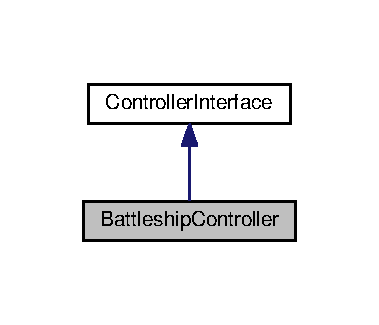
\includegraphics[width=182pt]{classBattleshipController__inherit__graph}
\end{center}
\end{figure}


Collaboration diagram for Battleship\+Controller\+:\nopagebreak
\begin{figure}[H]
\begin{center}
\leavevmode
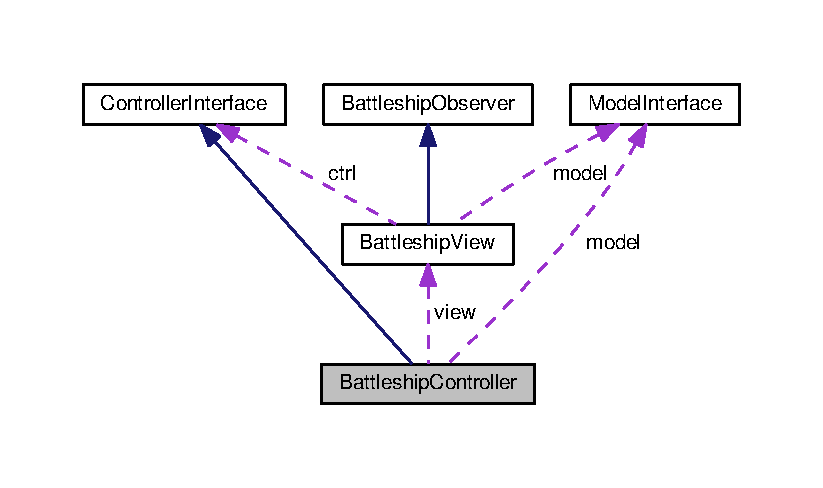
\includegraphics[width=350pt]{classBattleshipController__coll__graph}
\end{center}
\end{figure}
\subsection*{Public Member Functions}
\begin{DoxyCompactItemize}
\item 
\hyperlink{classBattleshipController_a49400b3ee3215b3cc3ee3252eb0e2c3c}{Battleship\+Controller} (\hyperlink{classModelInterface}{Model\+Interface} \&\hyperlink{classBattleshipController_a9253735219a238f80643188b190e90ce}{model})
\item 
void \hyperlink{classBattleshipController_a37949c2d70eb648a5957f9e60e86085c}{start\+New\+Game\+As\+Host} (const Q\+String \&player\+Name, const Q\+String \&age) override
\item 
void \hyperlink{classBattleshipController_a97013c1a4017c85bcc654424208a0cb4}{start\+New\+Game\+As\+Guest} (const Q\+String \&address, const Q\+String \&port, const Q\+String \&player\+Name, const Q\+String \&age) override
\end{DoxyCompactItemize}
\subsection*{Private Attributes}
\begin{DoxyCompactItemize}
\item 
\hyperlink{classModelInterface}{Model\+Interface} \& \hyperlink{classBattleshipController_a9253735219a238f80643188b190e90ce}{model}
\item 
\hyperlink{classGUI_1_1BattleshipView}{G\+U\+I\+::\+Battleship\+View} \hyperlink{classBattleshipController_a2fe88ba65554ddc67524f04c82812c27}{view}
\end{DoxyCompactItemize}


\subsection{Detailed Description}
Provides model data to the view and interprets user actions. 

\subsection{Constructor \& Destructor Documentation}
\index{Battleship\+Controller@{Battleship\+Controller}!Battleship\+Controller@{Battleship\+Controller}}
\index{Battleship\+Controller@{Battleship\+Controller}!Battleship\+Controller@{Battleship\+Controller}}
\subsubsection[{\texorpdfstring{Battleship\+Controller(\+Model\+Interface \&model)}{BattleshipController(ModelInterface &model)}}]{\setlength{\rightskip}{0pt plus 5cm}{\bf Battleship\+Controller} (
\begin{DoxyParamCaption}
\item[{{\bf Model\+Interface} \&}]{model}
\end{DoxyParamCaption}
)\hspace{0.3cm}{\ttfamily [explicit]}}\hypertarget{classBattleshipController_a49400b3ee3215b3cc3ee3252eb0e2c3c}{}\label{classBattleshipController_a49400b3ee3215b3cc3ee3252eb0e2c3c}


\subsection{Member Function Documentation}
\index{Battleship\+Controller@{Battleship\+Controller}!start\+New\+Game\+As\+Guest@{start\+New\+Game\+As\+Guest}}
\index{start\+New\+Game\+As\+Guest@{start\+New\+Game\+As\+Guest}!Battleship\+Controller@{Battleship\+Controller}}
\subsubsection[{\texorpdfstring{start\+New\+Game\+As\+Guest(const Q\+String \&address, const Q\+String \&port, const Q\+String \&player\+Name, const Q\+String \&age) override}{startNewGameAsGuest(const QString &address, const QString &port, const QString &playerName, const QString &age) override}}]{\setlength{\rightskip}{0pt plus 5cm}void start\+New\+Game\+As\+Guest (
\begin{DoxyParamCaption}
\item[{const Q\+String \&}]{address, }
\item[{const Q\+String \&}]{port, }
\item[{const Q\+String \&}]{player\+Name, }
\item[{const Q\+String \&}]{age}
\end{DoxyParamCaption}
)\hspace{0.3cm}{\ttfamily [override]}, {\ttfamily [virtual]}}\hypertarget{classBattleshipController_a97013c1a4017c85bcc654424208a0cb4}{}\label{classBattleshipController_a97013c1a4017c85bcc654424208a0cb4}
\begin{DoxySeeAlso}{See also}
Model\+Interface\+::start\+New\+Game\+As\+Guest(const std\+::string\&, int, const std\+::string\&, int) 
\end{DoxySeeAlso}


Implements \hyperlink{classControllerInterface_a59fe7601f2d7853043c7056d892b86a4}{Controller\+Interface}.

\index{Battleship\+Controller@{Battleship\+Controller}!start\+New\+Game\+As\+Host@{start\+New\+Game\+As\+Host}}
\index{start\+New\+Game\+As\+Host@{start\+New\+Game\+As\+Host}!Battleship\+Controller@{Battleship\+Controller}}
\subsubsection[{\texorpdfstring{start\+New\+Game\+As\+Host(const Q\+String \&player\+Name, const Q\+String \&age) override}{startNewGameAsHost(const QString &playerName, const QString &age) override}}]{\setlength{\rightskip}{0pt plus 5cm}void start\+New\+Game\+As\+Host (
\begin{DoxyParamCaption}
\item[{const Q\+String \&}]{player\+Name, }
\item[{const Q\+String \&}]{age}
\end{DoxyParamCaption}
)\hspace{0.3cm}{\ttfamily [override]}, {\ttfamily [virtual]}}\hypertarget{classBattleshipController_a37949c2d70eb648a5957f9e60e86085c}{}\label{classBattleshipController_a37949c2d70eb648a5957f9e60e86085c}
\begin{DoxySeeAlso}{See also}
Model\+Interface\+::start\+New\+Game\+As\+Host(const std\+::string\&, int) 
\end{DoxySeeAlso}


Implements \hyperlink{classControllerInterface_a0a1077ca83efdd21ffe8b1c042eb9b3b}{Controller\+Interface}.



\subsection{Member Data Documentation}
\index{Battleship\+Controller@{Battleship\+Controller}!model@{model}}
\index{model@{model}!Battleship\+Controller@{Battleship\+Controller}}
\subsubsection[{\texorpdfstring{model}{model}}]{\setlength{\rightskip}{0pt plus 5cm}{\bf Model\+Interface}\& model\hspace{0.3cm}{\ttfamily [private]}}\hypertarget{classBattleshipController_a9253735219a238f80643188b190e90ce}{}\label{classBattleshipController_a9253735219a238f80643188b190e90ce}
\index{Battleship\+Controller@{Battleship\+Controller}!view@{view}}
\index{view@{view}!Battleship\+Controller@{Battleship\+Controller}}
\subsubsection[{\texorpdfstring{view}{view}}]{\setlength{\rightskip}{0pt plus 5cm}{\bf G\+U\+I\+::\+Battleship\+View} view\hspace{0.3cm}{\ttfamily [private]}}\hypertarget{classBattleshipController_a2fe88ba65554ddc67524f04c82812c27}{}\label{classBattleshipController_a2fe88ba65554ddc67524f04c82812c27}


The documentation for this class was generated from the following files\+:\begin{DoxyCompactItemize}
\item 
\hyperlink{battleship__controller_8h}{battleship\+\_\+controller.\+h}\item 
\hyperlink{battleship__controller_8cpp}{battleship\+\_\+controller.\+cpp}\end{DoxyCompactItemize}

\hypertarget{classMODEL_1_1BattleshipModel}{}\section{Battleship\+Model Class Reference}
\label{classMODEL_1_1BattleshipModel}\index{Battleship\+Model@{Battleship\+Model}}


acts primarely as a wrapper around \hyperlink{classMODEL_1_1Game}{M\+O\+D\+E\+L\+::\+Game} class. Especially we make use of its constructor \& destructor. And we can dynamicallly switch between Host and Guest if so desired  




{\ttfamily \#include $<$battleship\+\_\+model.\+h$>$}



Inheritance diagram for Battleship\+Model\+:\nopagebreak
\begin{figure}[H]
\begin{center}
\leavevmode
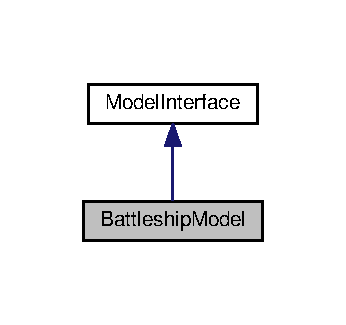
\includegraphics[width=166pt]{classMODEL_1_1BattleshipModel__inherit__graph}
\end{center}
\end{figure}


Collaboration diagram for Battleship\+Model\+:\nopagebreak
\begin{figure}[H]
\begin{center}
\leavevmode
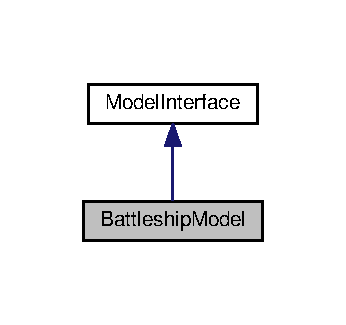
\includegraphics[width=166pt]{classMODEL_1_1BattleshipModel__coll__graph}
\end{center}
\end{figure}
\subsection*{Public Member Functions}
\begin{DoxyCompactItemize}
\item 
\hyperlink{classMODEL_1_1BattleshipModel_a8a7bef3348e68cf0267e79b445b94568}{Battleship\+Model} ()
\item 
\hyperlink{classMODEL_1_1BattleshipModel_aa5e22efe2dea484de9864a5a76b1c9f4}{$\sim$\+Battleship\+Model} ()
\item 
\hyperlink{classMODEL_1_1BattleshipModel_a7b959ebae2e8f6a5cf5a58aad6ee1676}{Battleship\+Model} (\hyperlink{classMODEL_1_1BattleshipModel}{Battleship\+Model} const \&)=delete
\item 
\hyperlink{classMODEL_1_1BattleshipModel}{Battleship\+Model} \& \hyperlink{classMODEL_1_1BattleshipModel_a6ba44e1437139bfe18033f0093e650db}{operator=} (\hyperlink{classMODEL_1_1BattleshipModel}{Battleship\+Model} const \&other)=delete
\item 
\hyperlink{classMODEL_1_1BattleshipModel_a6320be6c1f48b3f910929ac0e4b8fa1e}{Battleship\+Model} (\hyperlink{classMODEL_1_1BattleshipModel}{Battleship\+Model} \&\&other)=delete
\item 
\hyperlink{classMODEL_1_1BattleshipModel}{Battleship\+Model} \& \hyperlink{classMODEL_1_1BattleshipModel_a959c97c06c66558cf04ad4d91c5b5578}{operator=} (\hyperlink{classMODEL_1_1BattleshipModel}{Battleship\+Model} \&\&other)=delete
\item 
void \hyperlink{classMODEL_1_1BattleshipModel_a1afa557183362f561ae105fa141941ea}{register\+Observer} (\hyperlink{classBattleshipObserver}{Battleship\+Observer} \&observer)
\item 
void \hyperlink{classMODEL_1_1BattleshipModel_a655da28525f6ac4d2d15da6808c538b9}{start\+New\+Game\+As\+Host} (\hyperlink{classUserInfo}{User\+Info} user\+Info) override
\item 
void \hyperlink{classMODEL_1_1BattleshipModel_a076ef235e6ff9708c2bc0c2a4dcc141b}{start\+New\+Game\+As\+Guest} (const std\+::string \&address, int port, \hyperlink{classUserInfo}{User\+Info} user\+Info) override
\item 
void \hyperlink{classMODEL_1_1BattleshipModel_aa7cd87fbe771e195626f19960095bded}{cancel\+Hosting} () override
\item 
void \hyperlink{classMODEL_1_1BattleshipModel_a6de4c3b25683e4774fc9b524aa8c7e6a}{place\+Ship} (\hyperlink{classMODEL_1_1Point}{M\+O\+D\+E\+L\+::\+Point} p1, \hyperlink{classMODEL_1_1Point}{M\+O\+D\+E\+L\+::\+Point} p2) override
\end{DoxyCompactItemize}
\subsection*{Private Attributes}
\begin{DoxyCompactItemize}
\item 
std\+::unique\+\_\+ptr$<$ \hyperlink{classMODEL_1_1Game}{M\+O\+D\+E\+L\+::\+Game} $>$ \hyperlink{classMODEL_1_1BattleshipModel_a0aa74e6001f9f220f57faf9443e9972f}{game} = nullptr
\item 
std\+::vector$<$ std\+::reference\+\_\+wrapper$<$ \hyperlink{classBattleshipObserver}{Battleship\+Observer} $>$ $>$ \hyperlink{classMODEL_1_1BattleshipModel_aa59628064f9d6059844ecaec72b885d2}{observer\+List}
\end{DoxyCompactItemize}


\subsection{Detailed Description}
acts primarely as a wrapper around \hyperlink{classMODEL_1_1Game}{M\+O\+D\+E\+L\+::\+Game} class. Especially we make use of its constructor \& destructor. And we can dynamicallly switch between Host and Guest if so desired 

\subsection{Constructor \& Destructor Documentation}
\index{M\+O\+D\+E\+L\+::\+Battleship\+Model@{M\+O\+D\+E\+L\+::\+Battleship\+Model}!Battleship\+Model@{Battleship\+Model}}
\index{Battleship\+Model@{Battleship\+Model}!M\+O\+D\+E\+L\+::\+Battleship\+Model@{M\+O\+D\+E\+L\+::\+Battleship\+Model}}
\subsubsection[{\texorpdfstring{Battleship\+Model()}{BattleshipModel()}}]{\setlength{\rightskip}{0pt plus 5cm}{\bf Battleship\+Model} (
\begin{DoxyParamCaption}
{}
\end{DoxyParamCaption}
)\hspace{0.3cm}{\ttfamily [explicit]}}\hypertarget{classMODEL_1_1BattleshipModel_a8a7bef3348e68cf0267e79b445b94568}{}\label{classMODEL_1_1BattleshipModel_a8a7bef3348e68cf0267e79b445b94568}
\index{M\+O\+D\+E\+L\+::\+Battleship\+Model@{M\+O\+D\+E\+L\+::\+Battleship\+Model}!````~Battleship\+Model@{$\sim$\+Battleship\+Model}}
\index{````~Battleship\+Model@{$\sim$\+Battleship\+Model}!M\+O\+D\+E\+L\+::\+Battleship\+Model@{M\+O\+D\+E\+L\+::\+Battleship\+Model}}
\subsubsection[{\texorpdfstring{$\sim$\+Battleship\+Model()}{~BattleshipModel()}}]{\setlength{\rightskip}{0pt plus 5cm}$\sim${\bf Battleship\+Model} (
\begin{DoxyParamCaption}
{}
\end{DoxyParamCaption}
)\hspace{0.3cm}{\ttfamily [inline]}}\hypertarget{classMODEL_1_1BattleshipModel_aa5e22efe2dea484de9864a5a76b1c9f4}{}\label{classMODEL_1_1BattleshipModel_aa5e22efe2dea484de9864a5a76b1c9f4}
\index{M\+O\+D\+E\+L\+::\+Battleship\+Model@{M\+O\+D\+E\+L\+::\+Battleship\+Model}!Battleship\+Model@{Battleship\+Model}}
\index{Battleship\+Model@{Battleship\+Model}!M\+O\+D\+E\+L\+::\+Battleship\+Model@{M\+O\+D\+E\+L\+::\+Battleship\+Model}}
\subsubsection[{\texorpdfstring{Battleship\+Model(\+Battleship\+Model const \&)=delete}{BattleshipModel(BattleshipModel const &)=delete}}]{\setlength{\rightskip}{0pt plus 5cm}{\bf Battleship\+Model} (
\begin{DoxyParamCaption}
\item[{{\bf Battleship\+Model} const \&}]{}
\end{DoxyParamCaption}
)\hspace{0.3cm}{\ttfamily [delete]}}\hypertarget{classMODEL_1_1BattleshipModel_a7b959ebae2e8f6a5cf5a58aad6ee1676}{}\label{classMODEL_1_1BattleshipModel_a7b959ebae2e8f6a5cf5a58aad6ee1676}
\index{M\+O\+D\+E\+L\+::\+Battleship\+Model@{M\+O\+D\+E\+L\+::\+Battleship\+Model}!Battleship\+Model@{Battleship\+Model}}
\index{Battleship\+Model@{Battleship\+Model}!M\+O\+D\+E\+L\+::\+Battleship\+Model@{M\+O\+D\+E\+L\+::\+Battleship\+Model}}
\subsubsection[{\texorpdfstring{Battleship\+Model(\+Battleship\+Model \&\&other)=delete}{BattleshipModel(BattleshipModel &&other)=delete}}]{\setlength{\rightskip}{0pt plus 5cm}{\bf Battleship\+Model} (
\begin{DoxyParamCaption}
\item[{{\bf Battleship\+Model} \&\&}]{other}
\end{DoxyParamCaption}
)\hspace{0.3cm}{\ttfamily [delete]}}\hypertarget{classMODEL_1_1BattleshipModel_a6320be6c1f48b3f910929ac0e4b8fa1e}{}\label{classMODEL_1_1BattleshipModel_a6320be6c1f48b3f910929ac0e4b8fa1e}


\subsection{Member Function Documentation}
\index{M\+O\+D\+E\+L\+::\+Battleship\+Model@{M\+O\+D\+E\+L\+::\+Battleship\+Model}!cancel\+Hosting@{cancel\+Hosting}}
\index{cancel\+Hosting@{cancel\+Hosting}!M\+O\+D\+E\+L\+::\+Battleship\+Model@{M\+O\+D\+E\+L\+::\+Battleship\+Model}}
\subsubsection[{\texorpdfstring{cancel\+Hosting() override}{cancelHosting() override}}]{\setlength{\rightskip}{0pt plus 5cm}void cancel\+Hosting (
\begin{DoxyParamCaption}
{}
\end{DoxyParamCaption}
)\hspace{0.3cm}{\ttfamily [override]}, {\ttfamily [virtual]}}\hypertarget{classMODEL_1_1BattleshipModel_aa7cd87fbe771e195626f19960095bded}{}\label{classMODEL_1_1BattleshipModel_aa7cd87fbe771e195626f19960095bded}
\begin{DoxySeeAlso}{See also}
\hyperlink{classModelInterface_a2bb725b2837f07c50718296b2acb9bd6}{Model\+Interface\+::cancel\+Hosting()} 
\end{DoxySeeAlso}


Implements \hyperlink{classModelInterface_a2bb725b2837f07c50718296b2acb9bd6}{Model\+Interface}.

\index{M\+O\+D\+E\+L\+::\+Battleship\+Model@{M\+O\+D\+E\+L\+::\+Battleship\+Model}!operator=@{operator=}}
\index{operator=@{operator=}!M\+O\+D\+E\+L\+::\+Battleship\+Model@{M\+O\+D\+E\+L\+::\+Battleship\+Model}}
\subsubsection[{\texorpdfstring{operator=(\+Battleship\+Model const \&other)=delete}{operator=(BattleshipModel const &other)=delete}}]{\setlength{\rightskip}{0pt plus 5cm}{\bf Battleship\+Model}\& operator= (
\begin{DoxyParamCaption}
\item[{{\bf Battleship\+Model} const \&}]{other}
\end{DoxyParamCaption}
)\hspace{0.3cm}{\ttfamily [delete]}}\hypertarget{classMODEL_1_1BattleshipModel_a6ba44e1437139bfe18033f0093e650db}{}\label{classMODEL_1_1BattleshipModel_a6ba44e1437139bfe18033f0093e650db}
\index{M\+O\+D\+E\+L\+::\+Battleship\+Model@{M\+O\+D\+E\+L\+::\+Battleship\+Model}!operator=@{operator=}}
\index{operator=@{operator=}!M\+O\+D\+E\+L\+::\+Battleship\+Model@{M\+O\+D\+E\+L\+::\+Battleship\+Model}}
\subsubsection[{\texorpdfstring{operator=(\+Battleship\+Model \&\&other)=delete}{operator=(BattleshipModel &&other)=delete}}]{\setlength{\rightskip}{0pt plus 5cm}{\bf Battleship\+Model}\& operator= (
\begin{DoxyParamCaption}
\item[{{\bf Battleship\+Model} \&\&}]{other}
\end{DoxyParamCaption}
)\hspace{0.3cm}{\ttfamily [delete]}}\hypertarget{classMODEL_1_1BattleshipModel_a959c97c06c66558cf04ad4d91c5b5578}{}\label{classMODEL_1_1BattleshipModel_a959c97c06c66558cf04ad4d91c5b5578}
\index{M\+O\+D\+E\+L\+::\+Battleship\+Model@{M\+O\+D\+E\+L\+::\+Battleship\+Model}!place\+Ship@{place\+Ship}}
\index{place\+Ship@{place\+Ship}!M\+O\+D\+E\+L\+::\+Battleship\+Model@{M\+O\+D\+E\+L\+::\+Battleship\+Model}}
\subsubsection[{\texorpdfstring{place\+Ship(\+M\+O\+D\+E\+L\+::\+Point p1, M\+O\+D\+E\+L\+::\+Point p2) override}{placeShip(MODEL::Point p1, MODEL::Point p2) override}}]{\setlength{\rightskip}{0pt plus 5cm}void place\+Ship (
\begin{DoxyParamCaption}
\item[{{\bf M\+O\+D\+E\+L\+::\+Point}}]{p1, }
\item[{{\bf M\+O\+D\+E\+L\+::\+Point}}]{p2}
\end{DoxyParamCaption}
)\hspace{0.3cm}{\ttfamily [override]}, {\ttfamily [virtual]}}\hypertarget{classMODEL_1_1BattleshipModel_a6de4c3b25683e4774fc9b524aa8c7e6a}{}\label{classMODEL_1_1BattleshipModel_a6de4c3b25683e4774fc9b524aa8c7e6a}
\begin{DoxySeeAlso}{See also}
\hyperlink{classModelInterface_aa708cd5411011ade34c2796b3f102612}{Model\+Interface\+::place\+Ship(\+M\+O\+D\+E\+L\+::\+Point, M\+O\+D\+E\+L\+::\+Point)} 
\end{DoxySeeAlso}


Implements \hyperlink{classModelInterface_aa708cd5411011ade34c2796b3f102612}{Model\+Interface}.

\index{M\+O\+D\+E\+L\+::\+Battleship\+Model@{M\+O\+D\+E\+L\+::\+Battleship\+Model}!register\+Observer@{register\+Observer}}
\index{register\+Observer@{register\+Observer}!M\+O\+D\+E\+L\+::\+Battleship\+Model@{M\+O\+D\+E\+L\+::\+Battleship\+Model}}
\subsubsection[{\texorpdfstring{register\+Observer(\+Battleship\+Observer \&observer)}{registerObserver(BattleshipObserver &observer)}}]{\setlength{\rightskip}{0pt plus 5cm}void register\+Observer (
\begin{DoxyParamCaption}
\item[{{\bf Battleship\+Observer} \&}]{observer}
\end{DoxyParamCaption}
)\hspace{0.3cm}{\ttfamily [virtual]}}\hypertarget{classMODEL_1_1BattleshipModel_a1afa557183362f561ae105fa141941ea}{}\label{classMODEL_1_1BattleshipModel_a1afa557183362f561ae105fa141941ea}
Observer pattern as a part of M\+V\+C-\/\+Pattern 
\begin{DoxyParams}{Parameters}
{\em observer} & is usally a gui, that reflects/shows state-\/changes of the model \\
\hline
\end{DoxyParams}


Implements \hyperlink{classModelInterface_a38d9c2d3c1b09f40910a7ad1aa1aace4}{Model\+Interface}.

\index{M\+O\+D\+E\+L\+::\+Battleship\+Model@{M\+O\+D\+E\+L\+::\+Battleship\+Model}!start\+New\+Game\+As\+Guest@{start\+New\+Game\+As\+Guest}}
\index{start\+New\+Game\+As\+Guest@{start\+New\+Game\+As\+Guest}!M\+O\+D\+E\+L\+::\+Battleship\+Model@{M\+O\+D\+E\+L\+::\+Battleship\+Model}}
\subsubsection[{\texorpdfstring{start\+New\+Game\+As\+Guest(const std\+::string \&address, int port, User\+Info user\+Info) override}{startNewGameAsGuest(const std::string &address, int port, UserInfo userInfo) override}}]{\setlength{\rightskip}{0pt plus 5cm}void start\+New\+Game\+As\+Guest (
\begin{DoxyParamCaption}
\item[{const std\+::string \&}]{address, }
\item[{int}]{port, }
\item[{{\bf User\+Info}}]{user\+Info}
\end{DoxyParamCaption}
)\hspace{0.3cm}{\ttfamily [override]}, {\ttfamily [virtual]}}\hypertarget{classMODEL_1_1BattleshipModel_a076ef235e6ff9708c2bc0c2a4dcc141b}{}\label{classMODEL_1_1BattleshipModel_a076ef235e6ff9708c2bc0c2a4dcc141b}
\begin{DoxySeeAlso}{See also}
Model\+Interface\+::start\+New\+Game\+As\+Guest(const std\+::string\&, int, const std\+::string\&, int) 
\end{DoxySeeAlso}


Implements \hyperlink{classModelInterface_aee662ec9439a2344dcd39a0b65dcf639}{Model\+Interface}.

\index{M\+O\+D\+E\+L\+::\+Battleship\+Model@{M\+O\+D\+E\+L\+::\+Battleship\+Model}!start\+New\+Game\+As\+Host@{start\+New\+Game\+As\+Host}}
\index{start\+New\+Game\+As\+Host@{start\+New\+Game\+As\+Host}!M\+O\+D\+E\+L\+::\+Battleship\+Model@{M\+O\+D\+E\+L\+::\+Battleship\+Model}}
\subsubsection[{\texorpdfstring{start\+New\+Game\+As\+Host(\+User\+Info user\+Info) override}{startNewGameAsHost(UserInfo userInfo) override}}]{\setlength{\rightskip}{0pt plus 5cm}void start\+New\+Game\+As\+Host (
\begin{DoxyParamCaption}
\item[{{\bf User\+Info}}]{user\+Info}
\end{DoxyParamCaption}
)\hspace{0.3cm}{\ttfamily [override]}, {\ttfamily [virtual]}}\hypertarget{classMODEL_1_1BattleshipModel_a655da28525f6ac4d2d15da6808c538b9}{}\label{classMODEL_1_1BattleshipModel_a655da28525f6ac4d2d15da6808c538b9}
\begin{DoxySeeAlso}{See also}
Model\+Interface\+::start\+New\+Game\+As\+Host(const std\+::string\&, int) 
\end{DoxySeeAlso}


Implements \hyperlink{classModelInterface_a36aeb8e4e01dd08fd0416f3269789b31}{Model\+Interface}.



\subsection{Member Data Documentation}
\index{M\+O\+D\+E\+L\+::\+Battleship\+Model@{M\+O\+D\+E\+L\+::\+Battleship\+Model}!game@{game}}
\index{game@{game}!M\+O\+D\+E\+L\+::\+Battleship\+Model@{M\+O\+D\+E\+L\+::\+Battleship\+Model}}
\subsubsection[{\texorpdfstring{game}{game}}]{\setlength{\rightskip}{0pt plus 5cm}std\+::unique\+\_\+ptr$<${\bf M\+O\+D\+E\+L\+::\+Game}$>$ game = nullptr\hspace{0.3cm}{\ttfamily [private]}}\hypertarget{classMODEL_1_1BattleshipModel_a0aa74e6001f9f220f57faf9443e9972f}{}\label{classMODEL_1_1BattleshipModel_a0aa74e6001f9f220f57faf9443e9972f}
\index{M\+O\+D\+E\+L\+::\+Battleship\+Model@{M\+O\+D\+E\+L\+::\+Battleship\+Model}!observer\+List@{observer\+List}}
\index{observer\+List@{observer\+List}!M\+O\+D\+E\+L\+::\+Battleship\+Model@{M\+O\+D\+E\+L\+::\+Battleship\+Model}}
\subsubsection[{\texorpdfstring{observer\+List}{observerList}}]{\setlength{\rightskip}{0pt plus 5cm}std\+::vector$<$std\+::reference\+\_\+wrapper$<${\bf Battleship\+Observer}$>$ $>$ observer\+List\hspace{0.3cm}{\ttfamily [private]}}\hypertarget{classMODEL_1_1BattleshipModel_aa59628064f9d6059844ecaec72b885d2}{}\label{classMODEL_1_1BattleshipModel_aa59628064f9d6059844ecaec72b885d2}


The documentation for this class was generated from the following files\+:\begin{DoxyCompactItemize}
\item 
model/\hyperlink{battleship__model_8h}{battleship\+\_\+model.\+h}\item 
model/\hyperlink{battleship__model_8cpp}{battleship\+\_\+model.\+cpp}\end{DoxyCompactItemize}

\hypertarget{classBattleshipObserver}{}\section{Battleship\+Observer Class Reference}
\label{classBattleshipObserver}\index{Battleship\+Observer@{Battleship\+Observer}}


A base interface class, includes methods, which communicate with model and gui.  




{\ttfamily \#include $<$battleship\+\_\+observer.\+h$>$}



Inheritance diagram for Battleship\+Observer\+:\nopagebreak
\begin{figure}[H]
\begin{center}
\leavevmode
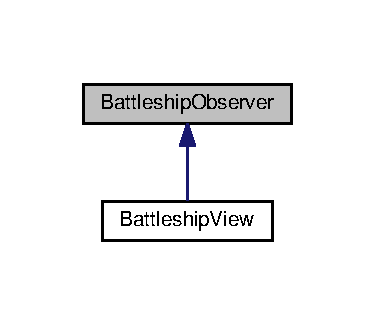
\includegraphics[width=180pt]{classBattleshipObserver__inherit__graph}
\end{center}
\end{figure}
\subsection*{Public Member Functions}
\begin{DoxyCompactItemize}
\item 
virtual \hyperlink{classBattleshipObserver_ad87d1278431b4b75b1e2e79eacf5a929}{$\sim$\+Battleship\+Observer} ()
\item 
virtual void \hyperlink{classBattleshipObserver_a54910db86473248c34d9a0149bdf9754}{ship\+Placement\+Started} ()=0
\end{DoxyCompactItemize}


\subsection{Detailed Description}
A base interface class, includes methods, which communicate with model and gui. 

\subsection{Constructor \& Destructor Documentation}
\index{Battleship\+Observer@{Battleship\+Observer}!````~Battleship\+Observer@{$\sim$\+Battleship\+Observer}}
\index{````~Battleship\+Observer@{$\sim$\+Battleship\+Observer}!Battleship\+Observer@{Battleship\+Observer}}
\subsubsection[{\texorpdfstring{$\sim$\+Battleship\+Observer()}{~BattleshipObserver()}}]{\setlength{\rightskip}{0pt plus 5cm}virtual $\sim${\bf Battleship\+Observer} (
\begin{DoxyParamCaption}
{}
\end{DoxyParamCaption}
)\hspace{0.3cm}{\ttfamily [inline]}, {\ttfamily [virtual]}}\hypertarget{classBattleshipObserver_ad87d1278431b4b75b1e2e79eacf5a929}{}\label{classBattleshipObserver_ad87d1278431b4b75b1e2e79eacf5a929}


\subsection{Member Function Documentation}
\index{Battleship\+Observer@{Battleship\+Observer}!ship\+Placement\+Started@{ship\+Placement\+Started}}
\index{ship\+Placement\+Started@{ship\+Placement\+Started}!Battleship\+Observer@{Battleship\+Observer}}
\subsubsection[{\texorpdfstring{ship\+Placement\+Started()=0}{shipPlacementStarted()=0}}]{\setlength{\rightskip}{0pt plus 5cm}virtual void ship\+Placement\+Started (
\begin{DoxyParamCaption}
{}
\end{DoxyParamCaption}
)\hspace{0.3cm}{\ttfamily [pure virtual]}}\hypertarget{classBattleshipObserver_a54910db86473248c34d9a0149bdf9754}{}\label{classBattleshipObserver_a54910db86473248c34d9a0149bdf9754}
after players connect to each other, they receive username of the opponent, timer starts (limited time for ship placement) and of course gui opens appropriate dialog/menu 

Implemented in \hyperlink{classGUI_1_1BattleshipView_a471a07ce060e70b1cfa03ce3674fba80}{Battleship\+View}.



The documentation for this class was generated from the following file\+:\begin{DoxyCompactItemize}
\item 
common/\hyperlink{battleship__observer_8h}{battleship\+\_\+observer.\+h}\end{DoxyCompactItemize}

\hypertarget{classGUI_1_1BattleshipView}{}\section{Battleship\+View Class Reference}
\label{classGUI_1_1BattleshipView}\index{Battleship\+View@{Battleship\+View}}


A simple class that defines and argument exception.  




{\ttfamily \#include $<$battleship\+\_\+view.\+h$>$}



Inheritance diagram for Battleship\+View\+:\nopagebreak
\begin{figure}[H]
\begin{center}
\leavevmode
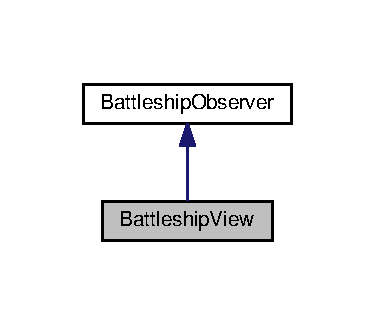
\includegraphics[width=180pt]{classGUI_1_1BattleshipView__inherit__graph}
\end{center}
\end{figure}


Collaboration diagram for Battleship\+View\+:\nopagebreak
\begin{figure}[H]
\begin{center}
\leavevmode
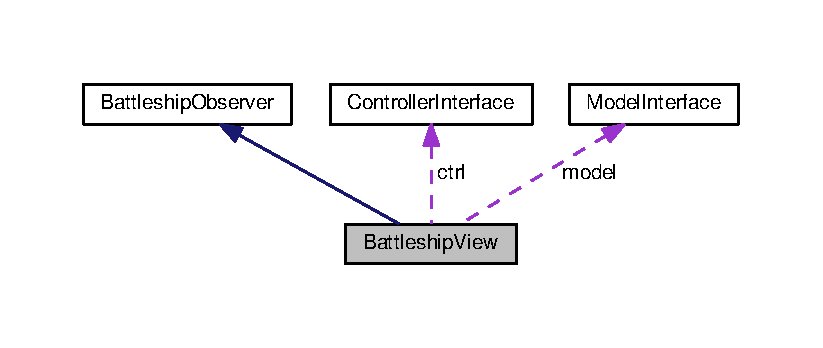
\includegraphics[width=350pt]{classGUI_1_1BattleshipView__coll__graph}
\end{center}
\end{figure}
\subsection*{Public Member Functions}
\begin{DoxyCompactItemize}
\item 
\hyperlink{classGUI_1_1BattleshipView_ac9fd11bfc017f0fe052608d297a5d457}{Battleship\+View} (\hyperlink{classModelInterface}{Model\+Interface} \&\hyperlink{classGUI_1_1BattleshipView_a9253735219a238f80643188b190e90ce}{model}, \hyperlink{classControllerInterface}{Controller\+Interface} \&controller)
\item 
void \hyperlink{classGUI_1_1BattleshipView_af7b5e55bee9a37cc4f9a861af40c120b}{show\+Error\+Message} (const std\+::string \&msg, const std\+::string \&title=\char`\"{}Oops, something went wrong\char`\"{})
\item 
void \hyperlink{classGUI_1_1BattleshipView_a511f6d90d37e864a1879eb6f5bd6f9cb}{show\+Waiting\+For\+Guest\+Connecting\+Dialog} ()
\item 
void \hyperlink{classGUI_1_1BattleshipView_aec4e5a4c453a3913c0a25435cfc92dd6}{close\+Top\+Dialog} ()
\item 
void \hyperlink{classGUI_1_1BattleshipView_a471a07ce060e70b1cfa03ce3674fba80}{ship\+Placement\+Started} ()
\end{DoxyCompactItemize}
\subsection*{Private Attributes}
\begin{DoxyCompactItemize}
\item 
\hyperlink{classModelInterface}{Model\+Interface} \& \hyperlink{classGUI_1_1BattleshipView_a9253735219a238f80643188b190e90ce}{model}
\item 
\hyperlink{classControllerInterface}{Controller\+Interface} \& \hyperlink{classGUI_1_1BattleshipView_a15e61471831211a4301410bdd802a4a4}{ctrl}
\item 
Q\+Dialog $\ast$ \hyperlink{classGUI_1_1BattleshipView_a08be9ec085bb0c3f19f8efe83902b4cb}{top\+Dialog} \{ nullptr \}
\end{DoxyCompactItemize}


\subsection{Detailed Description}
A simple class that defines and argument exception. 

\subsection{Constructor \& Destructor Documentation}
\index{G\+U\+I\+::\+Battleship\+View@{G\+U\+I\+::\+Battleship\+View}!Battleship\+View@{Battleship\+View}}
\index{Battleship\+View@{Battleship\+View}!G\+U\+I\+::\+Battleship\+View@{G\+U\+I\+::\+Battleship\+View}}
\subsubsection[{\texorpdfstring{Battleship\+View(\+Model\+Interface \&model, Controller\+Interface \&controller)}{BattleshipView(ModelInterface &model, ControllerInterface &controller)}}]{\setlength{\rightskip}{0pt plus 5cm}{\bf Battleship\+View} (
\begin{DoxyParamCaption}
\item[{{\bf Model\+Interface} \&}]{model, }
\item[{{\bf Controller\+Interface} \&}]{ctrl}
\end{DoxyParamCaption}
)\hspace{0.3cm}{\ttfamily [explicit]}}\hypertarget{classGUI_1_1BattleshipView_ac9fd11bfc017f0fe052608d297a5d457}{}\label{classGUI_1_1BattleshipView_ac9fd11bfc017f0fe052608d297a5d457}
Application begins with \hyperlink{classGUI_1_1PlayerForm}{Player\+Form} Dialog asking user for his name 

\subsection{Member Function Documentation}
\index{G\+U\+I\+::\+Battleship\+View@{G\+U\+I\+::\+Battleship\+View}!close\+Top\+Dialog@{close\+Top\+Dialog}}
\index{close\+Top\+Dialog@{close\+Top\+Dialog}!G\+U\+I\+::\+Battleship\+View@{G\+U\+I\+::\+Battleship\+View}}
\subsubsection[{\texorpdfstring{close\+Top\+Dialog()}{closeTopDialog()}}]{\setlength{\rightskip}{0pt plus 5cm}void close\+Top\+Dialog (
\begin{DoxyParamCaption}
{}
\end{DoxyParamCaption}
)}\hypertarget{classGUI_1_1BattleshipView_aec4e5a4c453a3913c0a25435cfc92dd6}{}\label{classGUI_1_1BattleshipView_aec4e5a4c453a3913c0a25435cfc92dd6}
closes top dialog programmatically, also without user having to click. Such dialog can be a popup informing about errors. \index{G\+U\+I\+::\+Battleship\+View@{G\+U\+I\+::\+Battleship\+View}!ship\+Placement\+Started@{ship\+Placement\+Started}}
\index{ship\+Placement\+Started@{ship\+Placement\+Started}!G\+U\+I\+::\+Battleship\+View@{G\+U\+I\+::\+Battleship\+View}}
\subsubsection[{\texorpdfstring{ship\+Placement\+Started()}{shipPlacementStarted()}}]{\setlength{\rightskip}{0pt plus 5cm}void ship\+Placement\+Started (
\begin{DoxyParamCaption}
{}
\end{DoxyParamCaption}
)\hspace{0.3cm}{\ttfamily [virtual]}}\hypertarget{classGUI_1_1BattleshipView_a471a07ce060e70b1cfa03ce3674fba80}{}\label{classGUI_1_1BattleshipView_a471a07ce060e70b1cfa03ce3674fba80}
\begin{DoxySeeAlso}{See also}
View\+Interface\+::show\+Waiting\+For\+Guest\+Connecting\+Dialog() 

View\+Interface\+::close\+Top\+Dialog() 

View\+Interface\+::show\+Error\+Message(const std\+::string\&, const std\+::string\&) 
\end{DoxySeeAlso}


Implements \hyperlink{classBattleshipObserver_a54910db86473248c34d9a0149bdf9754}{Battleship\+Observer}.

\index{G\+U\+I\+::\+Battleship\+View@{G\+U\+I\+::\+Battleship\+View}!show\+Error\+Message@{show\+Error\+Message}}
\index{show\+Error\+Message@{show\+Error\+Message}!G\+U\+I\+::\+Battleship\+View@{G\+U\+I\+::\+Battleship\+View}}
\subsubsection[{\texorpdfstring{show\+Error\+Message(const std\+::string \&msg, const std\+::string \&title=""Oops, something went wrong"")}{showErrorMessage(const std::string &msg, const std::string &title="Oops, something went wrong")}}]{\setlength{\rightskip}{0pt plus 5cm}void show\+Error\+Message (
\begin{DoxyParamCaption}
\item[{const std\+::string \&}]{msg, }
\item[{const std\+::string \&}]{title = {\ttfamily \char`\"{}Oops,~something~went~wrong\char`\"{}}}
\end{DoxyParamCaption}
)}\hypertarget{classGUI_1_1BattleshipView_af7b5e55bee9a37cc4f9a861af40c120b}{}\label{classGUI_1_1BattleshipView_af7b5e55bee9a37cc4f9a861af40c120b}

\begin{DoxyParams}{Parameters}
{\em msg} & actual error message message \\
\hline
{\em title} & title of the window like Q\+Message\+Box \\
\hline
\end{DoxyParams}
\index{G\+U\+I\+::\+Battleship\+View@{G\+U\+I\+::\+Battleship\+View}!show\+Waiting\+For\+Guest\+Connecting\+Dialog@{show\+Waiting\+For\+Guest\+Connecting\+Dialog}}
\index{show\+Waiting\+For\+Guest\+Connecting\+Dialog@{show\+Waiting\+For\+Guest\+Connecting\+Dialog}!G\+U\+I\+::\+Battleship\+View@{G\+U\+I\+::\+Battleship\+View}}
\subsubsection[{\texorpdfstring{show\+Waiting\+For\+Guest\+Connecting\+Dialog()}{showWaitingForGuestConnectingDialog()}}]{\setlength{\rightskip}{0pt plus 5cm}void show\+Waiting\+For\+Guest\+Connecting\+Dialog (
\begin{DoxyParamCaption}
{}
\end{DoxyParamCaption}
)}\hypertarget{classGUI_1_1BattleshipView_a511f6d90d37e864a1879eb6f5bd6f9cb}{}\label{classGUI_1_1BattleshipView_a511f6d90d37e864a1879eb6f5bd6f9cb}
inform user that he has to be patient. Being patient is always good... well at least for someone. 

\subsection{Member Data Documentation}
\index{G\+U\+I\+::\+Battleship\+View@{G\+U\+I\+::\+Battleship\+View}!ctrl@{ctrl}}
\index{ctrl@{ctrl}!G\+U\+I\+::\+Battleship\+View@{G\+U\+I\+::\+Battleship\+View}}
\subsubsection[{\texorpdfstring{ctrl}{ctrl}}]{\setlength{\rightskip}{0pt plus 5cm}{\bf Controller\+Interface}\& ctrl\hspace{0.3cm}{\ttfamily [private]}}\hypertarget{classGUI_1_1BattleshipView_a15e61471831211a4301410bdd802a4a4}{}\label{classGUI_1_1BattleshipView_a15e61471831211a4301410bdd802a4a4}
\index{G\+U\+I\+::\+Battleship\+View@{G\+U\+I\+::\+Battleship\+View}!model@{model}}
\index{model@{model}!G\+U\+I\+::\+Battleship\+View@{G\+U\+I\+::\+Battleship\+View}}
\subsubsection[{\texorpdfstring{model}{model}}]{\setlength{\rightskip}{0pt plus 5cm}{\bf Model\+Interface}\& model\hspace{0.3cm}{\ttfamily [private]}}\hypertarget{classGUI_1_1BattleshipView_a9253735219a238f80643188b190e90ce}{}\label{classGUI_1_1BattleshipView_a9253735219a238f80643188b190e90ce}
\index{G\+U\+I\+::\+Battleship\+View@{G\+U\+I\+::\+Battleship\+View}!top\+Dialog@{top\+Dialog}}
\index{top\+Dialog@{top\+Dialog}!G\+U\+I\+::\+Battleship\+View@{G\+U\+I\+::\+Battleship\+View}}
\subsubsection[{\texorpdfstring{top\+Dialog}{topDialog}}]{\setlength{\rightskip}{0pt plus 5cm}Q\+Dialog$\ast$ top\+Dialog \{ nullptr \}\hspace{0.3cm}{\ttfamily [private]}}\hypertarget{classGUI_1_1BattleshipView_a08be9ec085bb0c3f19f8efe83902b4cb}{}\label{classGUI_1_1BattleshipView_a08be9ec085bb0c3f19f8efe83902b4cb}


The documentation for this class was generated from the following files\+:\begin{DoxyCompactItemize}
\item 
gui/\hyperlink{battleship__view_8h}{battleship\+\_\+view.\+h}\item 
gui/\hyperlink{battleship__view_8cpp}{battleship\+\_\+view.\+cpp}\end{DoxyCompactItemize}

\hypertarget{classMODEL_1_1Communicator}{}\section{Communicator Class Reference}
\label{classMODEL_1_1Communicator}\index{Communicator@{Communicator}}


A class that uses \hyperlink{classMODEL_1_1Connection}{Connection} to recieve/send encoded/decoded information stored in json objects.  




{\ttfamily \#include $<$communicator.\+h$>$}



Collaboration diagram for Communicator\+:\nopagebreak
\begin{figure}[H]
\begin{center}
\leavevmode
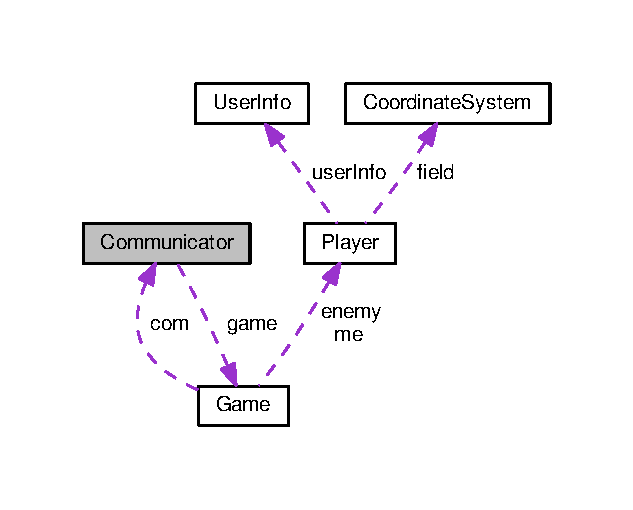
\includegraphics[width=304pt]{classMODEL_1_1Communicator__coll__graph}
\end{center}
\end{figure}
\subsection*{Public Member Functions}
\begin{DoxyCompactItemize}
\item 
\hyperlink{classMODEL_1_1Communicator_a2993409e2e41d9363c76e59b054df1ed}{Communicator} (\hyperlink{classMODEL_1_1Game}{M\+O\+D\+E\+L\+::\+Game} \&\hyperlink{classMODEL_1_1Communicator_a1018ef7ed7f7714ef648545d209b9ff4}{game}, const std\+::string \&address, int port, std\+::function$<$ void()$>$ callback\+On\+Connected)
\item 
\hyperlink{classMODEL_1_1Communicator_ad11952ffbf95dda14e718d936e26aa1c}{Communicator} (\hyperlink{classMODEL_1_1Game}{M\+O\+D\+E\+L\+::\+Game} \&\hyperlink{classMODEL_1_1Communicator_a1018ef7ed7f7714ef648545d209b9ff4}{game}, std\+::function$<$ void()$>$ callback\+On\+Connected)
\item 
\hyperlink{classMODEL_1_1Communicator_ae1ebbaf619b559917bb5d0508c604883}{Communicator} (\hyperlink{classMODEL_1_1Communicator}{Communicator} const \&)=delete
\item 
\hyperlink{classMODEL_1_1Communicator}{Communicator} \& \hyperlink{classMODEL_1_1Communicator_a92705f86fea309452a1da1eb027577e9}{operator=} (\hyperlink{classMODEL_1_1Communicator}{Communicator} const \&other)=delete
\item 
\hyperlink{classMODEL_1_1Communicator_a9354967a93e7ec6136a5c8ece2e755d2}{Communicator} (\hyperlink{classMODEL_1_1Communicator}{Communicator} \&\&other)=delete
\item 
\hyperlink{classMODEL_1_1Communicator}{Communicator} \& \hyperlink{classMODEL_1_1Communicator_ae0fb22dd825e3817b1a5d1846f916197}{operator=} (\hyperlink{classMODEL_1_1Communicator}{Communicator} \&\&other)=delete
\item 
void \hyperlink{classMODEL_1_1Communicator_addda61885a1ef23ed692f15ca56f43c3}{send\+User\+Info} (const \hyperlink{classUserInfo}{User\+Info} \&user\+Info)
\end{DoxyCompactItemize}
\subsection*{Private Member Functions}
\begin{DoxyCompactItemize}
\item 
void \hyperlink{classMODEL_1_1Communicator_a7bf1372fe11b00605a91dccdf336e81d}{data\+Received} (const Q\+Byte\+Array \&data)
\item 
void \hyperlink{classMODEL_1_1Communicator_ab9ff7c65f14065e5bdad9cfc7e15ba27}{send\+Json} (const \hyperlink{namespaceMODEL_a2afce0a47a93eee73a314d53e4890153}{Command} \&command, const Q\+Json\+Object \&json)
\end{DoxyCompactItemize}
\subsection*{Private Attributes}
\begin{DoxyCompactItemize}
\item 
\hyperlink{classMODEL_1_1Game}{Game} \& \hyperlink{classMODEL_1_1Communicator_a1018ef7ed7f7714ef648545d209b9ff4}{game}
\item 
std\+::unique\+\_\+ptr$<$ \hyperlink{classMODEL_1_1Connection}{Connection} $>$ \hyperlink{classMODEL_1_1Communicator_a74211040c2e2fd8475ce5f579c906171}{conn}
\end{DoxyCompactItemize}


\subsection{Detailed Description}
A class that uses \hyperlink{classMODEL_1_1Connection}{Connection} to recieve/send encoded/decoded information stored in json objects. 

\subsection{Constructor \& Destructor Documentation}
\index{M\+O\+D\+E\+L\+::\+Communicator@{M\+O\+D\+E\+L\+::\+Communicator}!Communicator@{Communicator}}
\index{Communicator@{Communicator}!M\+O\+D\+E\+L\+::\+Communicator@{M\+O\+D\+E\+L\+::\+Communicator}}
\subsubsection[{\texorpdfstring{Communicator(\+M\+O\+D\+E\+L\+::\+Game \&game, const std\+::string \&address, int port, std\+::function$<$ void()$>$ callback\+On\+Connected)}{Communicator(MODEL::Game &game, const std::string &address, int port, std::function< void()> callbackOnConnected)}}]{\setlength{\rightskip}{0pt plus 5cm}{\bf Communicator} (
\begin{DoxyParamCaption}
\item[{{\bf M\+O\+D\+E\+L\+::\+Game} \&}]{game, }
\item[{const std\+::string \&}]{address, }
\item[{int}]{port, }
\item[{std\+::function$<$ void()$>$}]{callback\+On\+Connected}
\end{DoxyParamCaption}
)\hspace{0.3cm}{\ttfamily [explicit]}}\hypertarget{classMODEL_1_1Communicator_a2993409e2e41d9363c76e59b054df1ed}{}\label{classMODEL_1_1Communicator_a2993409e2e41d9363c76e59b054df1ed}
creates commincator as guest


\begin{DoxyParams}{Parameters}
{\em callback\+On\+Connected} & called when connection is established \\
\hline
\end{DoxyParams}
\index{M\+O\+D\+E\+L\+::\+Communicator@{M\+O\+D\+E\+L\+::\+Communicator}!Communicator@{Communicator}}
\index{Communicator@{Communicator}!M\+O\+D\+E\+L\+::\+Communicator@{M\+O\+D\+E\+L\+::\+Communicator}}
\subsubsection[{\texorpdfstring{Communicator(\+M\+O\+D\+E\+L\+::\+Game \&game, std\+::function$<$ void()$>$ callback\+On\+Connected)}{Communicator(MODEL::Game &game, std::function< void()> callbackOnConnected)}}]{\setlength{\rightskip}{0pt plus 5cm}{\bf Communicator} (
\begin{DoxyParamCaption}
\item[{{\bf M\+O\+D\+E\+L\+::\+Game} \&}]{game, }
\item[{std\+::function$<$ void()$>$}]{callback\+On\+Connected}
\end{DoxyParamCaption}
)\hspace{0.3cm}{\ttfamily [explicit]}}\hypertarget{classMODEL_1_1Communicator_ad11952ffbf95dda14e718d936e26aa1c}{}\label{classMODEL_1_1Communicator_ad11952ffbf95dda14e718d936e26aa1c}
creates commincator as host


\begin{DoxyParams}{Parameters}
{\em callback\+On\+Connected} & called when connection is established \\
\hline
\end{DoxyParams}
\index{M\+O\+D\+E\+L\+::\+Communicator@{M\+O\+D\+E\+L\+::\+Communicator}!Communicator@{Communicator}}
\index{Communicator@{Communicator}!M\+O\+D\+E\+L\+::\+Communicator@{M\+O\+D\+E\+L\+::\+Communicator}}
\subsubsection[{\texorpdfstring{Communicator(\+Communicator const \&)=delete}{Communicator(Communicator const &)=delete}}]{\setlength{\rightskip}{0pt plus 5cm}{\bf Communicator} (
\begin{DoxyParamCaption}
\item[{{\bf Communicator} const \&}]{}
\end{DoxyParamCaption}
)\hspace{0.3cm}{\ttfamily [delete]}}\hypertarget{classMODEL_1_1Communicator_ae1ebbaf619b559917bb5d0508c604883}{}\label{classMODEL_1_1Communicator_ae1ebbaf619b559917bb5d0508c604883}
\index{M\+O\+D\+E\+L\+::\+Communicator@{M\+O\+D\+E\+L\+::\+Communicator}!Communicator@{Communicator}}
\index{Communicator@{Communicator}!M\+O\+D\+E\+L\+::\+Communicator@{M\+O\+D\+E\+L\+::\+Communicator}}
\subsubsection[{\texorpdfstring{Communicator(\+Communicator \&\&other)=delete}{Communicator(Communicator &&other)=delete}}]{\setlength{\rightskip}{0pt plus 5cm}{\bf Communicator} (
\begin{DoxyParamCaption}
\item[{{\bf Communicator} \&\&}]{other}
\end{DoxyParamCaption}
)\hspace{0.3cm}{\ttfamily [delete]}}\hypertarget{classMODEL_1_1Communicator_a9354967a93e7ec6136a5c8ece2e755d2}{}\label{classMODEL_1_1Communicator_a9354967a93e7ec6136a5c8ece2e755d2}


\subsection{Member Function Documentation}
\index{M\+O\+D\+E\+L\+::\+Communicator@{M\+O\+D\+E\+L\+::\+Communicator}!data\+Received@{data\+Received}}
\index{data\+Received@{data\+Received}!M\+O\+D\+E\+L\+::\+Communicator@{M\+O\+D\+E\+L\+::\+Communicator}}
\subsubsection[{\texorpdfstring{data\+Received(const Q\+Byte\+Array \&data)}{dataReceived(const QByteArray &data)}}]{\setlength{\rightskip}{0pt plus 5cm}void data\+Received (
\begin{DoxyParamCaption}
\item[{const Q\+Byte\+Array \&}]{data}
\end{DoxyParamCaption}
)\hspace{0.3cm}{\ttfamily [private]}}\hypertarget{classMODEL_1_1Communicator_a7bf1372fe11b00605a91dccdf336e81d}{}\label{classMODEL_1_1Communicator_a7bf1372fe11b00605a91dccdf336e81d}
\index{M\+O\+D\+E\+L\+::\+Communicator@{M\+O\+D\+E\+L\+::\+Communicator}!operator=@{operator=}}
\index{operator=@{operator=}!M\+O\+D\+E\+L\+::\+Communicator@{M\+O\+D\+E\+L\+::\+Communicator}}
\subsubsection[{\texorpdfstring{operator=(\+Communicator const \&other)=delete}{operator=(Communicator const &other)=delete}}]{\setlength{\rightskip}{0pt plus 5cm}{\bf Communicator}\& operator= (
\begin{DoxyParamCaption}
\item[{{\bf Communicator} const \&}]{other}
\end{DoxyParamCaption}
)\hspace{0.3cm}{\ttfamily [delete]}}\hypertarget{classMODEL_1_1Communicator_a92705f86fea309452a1da1eb027577e9}{}\label{classMODEL_1_1Communicator_a92705f86fea309452a1da1eb027577e9}
\index{M\+O\+D\+E\+L\+::\+Communicator@{M\+O\+D\+E\+L\+::\+Communicator}!operator=@{operator=}}
\index{operator=@{operator=}!M\+O\+D\+E\+L\+::\+Communicator@{M\+O\+D\+E\+L\+::\+Communicator}}
\subsubsection[{\texorpdfstring{operator=(\+Communicator \&\&other)=delete}{operator=(Communicator &&other)=delete}}]{\setlength{\rightskip}{0pt plus 5cm}{\bf Communicator}\& operator= (
\begin{DoxyParamCaption}
\item[{{\bf Communicator} \&\&}]{other}
\end{DoxyParamCaption}
)\hspace{0.3cm}{\ttfamily [delete]}}\hypertarget{classMODEL_1_1Communicator_ae0fb22dd825e3817b1a5d1846f916197}{}\label{classMODEL_1_1Communicator_ae0fb22dd825e3817b1a5d1846f916197}
\index{M\+O\+D\+E\+L\+::\+Communicator@{M\+O\+D\+E\+L\+::\+Communicator}!send\+Json@{send\+Json}}
\index{send\+Json@{send\+Json}!M\+O\+D\+E\+L\+::\+Communicator@{M\+O\+D\+E\+L\+::\+Communicator}}
\subsubsection[{\texorpdfstring{send\+Json(const Command \&command, const Q\+Json\+Object \&json)}{sendJson(const Command &command, const QJsonObject &json)}}]{\setlength{\rightskip}{0pt plus 5cm}void send\+Json (
\begin{DoxyParamCaption}
\item[{const {\bf Command} \&}]{command, }
\item[{const Q\+Json\+Object \&}]{json}
\end{DoxyParamCaption}
)\hspace{0.3cm}{\ttfamily [private]}}\hypertarget{classMODEL_1_1Communicator_ab9ff7c65f14065e5bdad9cfc7e15ba27}{}\label{classMODEL_1_1Communicator_ab9ff7c65f14065e5bdad9cfc7e15ba27}
\index{M\+O\+D\+E\+L\+::\+Communicator@{M\+O\+D\+E\+L\+::\+Communicator}!send\+User\+Info@{send\+User\+Info}}
\index{send\+User\+Info@{send\+User\+Info}!M\+O\+D\+E\+L\+::\+Communicator@{M\+O\+D\+E\+L\+::\+Communicator}}
\subsubsection[{\texorpdfstring{send\+User\+Info(const User\+Info \&user\+Info)}{sendUserInfo(const UserInfo &userInfo)}}]{\setlength{\rightskip}{0pt plus 5cm}void send\+User\+Info (
\begin{DoxyParamCaption}
\item[{const {\bf User\+Info} \&}]{user\+Info}
\end{DoxyParamCaption}
)}\hypertarget{classMODEL_1_1Communicator_addda61885a1ef23ed692f15ca56f43c3}{}\label{classMODEL_1_1Communicator_addda61885a1ef23ed692f15ca56f43c3}


\subsection{Member Data Documentation}
\index{M\+O\+D\+E\+L\+::\+Communicator@{M\+O\+D\+E\+L\+::\+Communicator}!conn@{conn}}
\index{conn@{conn}!M\+O\+D\+E\+L\+::\+Communicator@{M\+O\+D\+E\+L\+::\+Communicator}}
\subsubsection[{\texorpdfstring{conn}{conn}}]{\setlength{\rightskip}{0pt plus 5cm}std\+::unique\+\_\+ptr$<${\bf Connection}$>$ conn\hspace{0.3cm}{\ttfamily [private]}}\hypertarget{classMODEL_1_1Communicator_a74211040c2e2fd8475ce5f579c906171}{}\label{classMODEL_1_1Communicator_a74211040c2e2fd8475ce5f579c906171}
\index{M\+O\+D\+E\+L\+::\+Communicator@{M\+O\+D\+E\+L\+::\+Communicator}!game@{game}}
\index{game@{game}!M\+O\+D\+E\+L\+::\+Communicator@{M\+O\+D\+E\+L\+::\+Communicator}}
\subsubsection[{\texorpdfstring{game}{game}}]{\setlength{\rightskip}{0pt plus 5cm}{\bf Game}\& game\hspace{0.3cm}{\ttfamily [private]}}\hypertarget{classMODEL_1_1Communicator_a1018ef7ed7f7714ef648545d209b9ff4}{}\label{classMODEL_1_1Communicator_a1018ef7ed7f7714ef648545d209b9ff4}


The documentation for this class was generated from the following files\+:\begin{DoxyCompactItemize}
\item 
model/\hyperlink{communicator_8h}{communicator.\+h}\item 
model/\hyperlink{communicator_8cpp}{communicator.\+cpp}\end{DoxyCompactItemize}

\hypertarget{classMODEL_1_1Connection}{}\section{Connection Class Reference}
\label{classMODEL_1_1Connection}\index{Connection@{Connection}}


A base class that defines the basic functions for connection.  




{\ttfamily \#include $<$connection.\+h$>$}



Inheritance diagram for Connection\+:\nopagebreak
\begin{figure}[H]
\begin{center}
\leavevmode
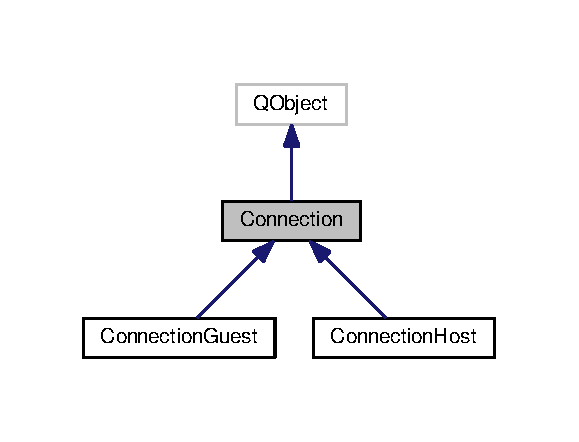
\includegraphics[width=278pt]{classMODEL_1_1Connection__inherit__graph}
\end{center}
\end{figure}


Collaboration diagram for Connection\+:\nopagebreak
\begin{figure}[H]
\begin{center}
\leavevmode
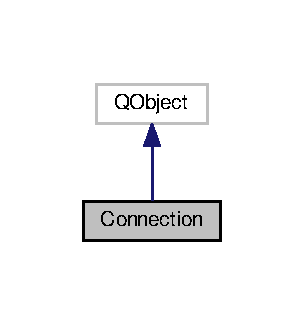
\includegraphics[width=146pt]{classMODEL_1_1Connection__coll__graph}
\end{center}
\end{figure}
\subsection*{Public Member Functions}
\begin{DoxyCompactItemize}
\item 
\hyperlink{classMODEL_1_1Connection_afde897e745ea37e60ff20b72a409a280}{Connection} (std\+::function$<$ void(const Q\+Byte\+Array \&)$>$ \hyperlink{classMODEL_1_1Connection_aa0b44072225e1b07b646bd973719ac80}{callback\+On\+Data\+Received}, std\+::function$<$ void()$>$ \hyperlink{classMODEL_1_1Connection_a0cb35149e127dbce2a09f0ac5d5cfc16}{callback\+On\+Connected}, Q\+Object $\ast$parent)
\item 
virtual \hyperlink{classMODEL_1_1Connection_a7a3e1a734e64796b393be72275bcb246}{$\sim$\+Connection} ()
\item 
\hyperlink{classMODEL_1_1Connection_adba016dc9c4adef32a776bce06277c44}{Connection} (\hyperlink{classMODEL_1_1Connection}{Connection} const \&)=delete
\item 
\hyperlink{classMODEL_1_1Connection}{Connection} \& \hyperlink{classMODEL_1_1Connection_a821cfec5ddc35d7ccb324adae37f82c4}{operator=} (\hyperlink{classMODEL_1_1Connection}{Connection} const \&other)=delete
\item 
\hyperlink{classMODEL_1_1Connection_a66608e31b9bba043aa4c7f11ecdda6ee}{Connection} (\hyperlink{classMODEL_1_1Connection}{Connection} \&\&other)=delete
\item 
\hyperlink{classMODEL_1_1Connection}{Connection} \& \hyperlink{classMODEL_1_1Connection_a4bef84588b92c963c1ad8ac70d67dc4c}{operator=} (\hyperlink{classMODEL_1_1Connection}{Connection} \&\&other)=delete
\item 
void \hyperlink{classMODEL_1_1Connection_ae31ebe57b25d10a93a635cad878834b0}{send\+Data} (const Q\+Byte\+Array \&data)
\end{DoxyCompactItemize}
\subsection*{Protected Member Functions}
\begin{DoxyCompactItemize}
\item 
void \hyperlink{classMODEL_1_1Connection_ab1703367762abc1490e00dcd5ccb29bc}{read\+Data} ()
\item 
void \hyperlink{classMODEL_1_1Connection_a37b4c359b4694947d5413d645feec8d5}{init\+Network\+Session} ()
\item 
virtual void \hyperlink{classMODEL_1_1Connection_ae3e484e0f3217ab38dbaa36f4a379f69}{begin\+Connecting} ()=0
\item 
void \hyperlink{classMODEL_1_1Connection_a4cc305570c43d0834291ef0b4c745c13}{display\+Error} (Q\+Abstract\+Socket\+::\+Socket\+Error socket\+Error)
\end{DoxyCompactItemize}
\subsection*{Protected Attributes}
\begin{DoxyCompactItemize}
\item 
Q\+Tcp\+Socket $\ast$ \hyperlink{classMODEL_1_1Connection_a0558920c8ed7149d80c3051117c2d60f}{socket} \{nullptr\}
\item 
quint16 \hyperlink{classMODEL_1_1Connection_a71471e77e7dd9a903dbd82687ca5c91c}{block\+Size} \{0\}
\item 
std\+::function$<$ void(const Q\+Byte\+Array \&)$>$ \hyperlink{classMODEL_1_1Connection_aa0b44072225e1b07b646bd973719ac80}{callback\+On\+Data\+Received}
\item 
std\+::function$<$ void()$>$ \hyperlink{classMODEL_1_1Connection_a0cb35149e127dbce2a09f0ac5d5cfc16}{callback\+On\+Connected}
\end{DoxyCompactItemize}
\subsection*{Private Slots}
\begin{DoxyCompactItemize}
\item 
void \hyperlink{classMODEL_1_1Connection_a29259cebd0636f7f03aafe1810b46e02}{session\+Opened} ()
\end{DoxyCompactItemize}
\subsection*{Private Attributes}
\begin{DoxyCompactItemize}
\item 
Q\+Network\+Session $\ast$ \hyperlink{classMODEL_1_1Connection_a24862c1b1d3d8d16843535cf9ec65dc2}{network\+Session} \{nullptr\}
\end{DoxyCompactItemize}


\subsection{Detailed Description}
A base class that defines the basic functions for connection. 

\subsection{Constructor \& Destructor Documentation}
\index{M\+O\+D\+E\+L\+::\+Connection@{M\+O\+D\+E\+L\+::\+Connection}!Connection@{Connection}}
\index{Connection@{Connection}!M\+O\+D\+E\+L\+::\+Connection@{M\+O\+D\+E\+L\+::\+Connection}}
\subsubsection[{\texorpdfstring{Connection(std\+::function$<$ void(const Q\+Byte\+Array \&)$>$ callback\+On\+Data\+Received, std\+::function$<$ void()$>$ callback\+On\+Connected, Q\+Object $\ast$parent)}{Connection(std::function< void(const QByteArray &)> callbackOnDataReceived, std::function< void()> callbackOnConnected, QObject *parent)}}]{\setlength{\rightskip}{0pt plus 5cm}{\bf Connection} (
\begin{DoxyParamCaption}
\item[{std\+::function$<$ void(const Q\+Byte\+Array \&)$>$}]{callback\+On\+Data\+Received, }
\item[{std\+::function$<$ void()$>$}]{callback\+On\+Connected, }
\item[{Q\+Object $\ast$}]{parent}
\end{DoxyParamCaption}
)\hspace{0.3cm}{\ttfamily [explicit]}}\hypertarget{classMODEL_1_1Connection_afde897e745ea37e60ff20b72a409a280}{}\label{classMODEL_1_1Connection_afde897e745ea37e60ff20b72a409a280}

\begin{DoxyParams}{Parameters}
{\em callback\+On\+Data\+Received} & called when full data blcock is received. \\
\hline
{\em callback\+On\+Connected} & called when connection is established \\
\hline
\end{DoxyParams}
\index{M\+O\+D\+E\+L\+::\+Connection@{M\+O\+D\+E\+L\+::\+Connection}!````~Connection@{$\sim$\+Connection}}
\index{````~Connection@{$\sim$\+Connection}!M\+O\+D\+E\+L\+::\+Connection@{M\+O\+D\+E\+L\+::\+Connection}}
\subsubsection[{\texorpdfstring{$\sim$\+Connection()}{~Connection()}}]{\setlength{\rightskip}{0pt plus 5cm}$\sim${\bf Connection} (
\begin{DoxyParamCaption}
{}
\end{DoxyParamCaption}
)\hspace{0.3cm}{\ttfamily [virtual]}}\hypertarget{classMODEL_1_1Connection_a7a3e1a734e64796b393be72275bcb246}{}\label{classMODEL_1_1Connection_a7a3e1a734e64796b393be72275bcb246}
\index{M\+O\+D\+E\+L\+::\+Connection@{M\+O\+D\+E\+L\+::\+Connection}!Connection@{Connection}}
\index{Connection@{Connection}!M\+O\+D\+E\+L\+::\+Connection@{M\+O\+D\+E\+L\+::\+Connection}}
\subsubsection[{\texorpdfstring{Connection(\+Connection const \&)=delete}{Connection(Connection const &)=delete}}]{\setlength{\rightskip}{0pt plus 5cm}{\bf Connection} (
\begin{DoxyParamCaption}
\item[{{\bf Connection} const \&}]{}
\end{DoxyParamCaption}
)\hspace{0.3cm}{\ttfamily [delete]}}\hypertarget{classMODEL_1_1Connection_adba016dc9c4adef32a776bce06277c44}{}\label{classMODEL_1_1Connection_adba016dc9c4adef32a776bce06277c44}
\index{M\+O\+D\+E\+L\+::\+Connection@{M\+O\+D\+E\+L\+::\+Connection}!Connection@{Connection}}
\index{Connection@{Connection}!M\+O\+D\+E\+L\+::\+Connection@{M\+O\+D\+E\+L\+::\+Connection}}
\subsubsection[{\texorpdfstring{Connection(\+Connection \&\&other)=delete}{Connection(Connection &&other)=delete}}]{\setlength{\rightskip}{0pt plus 5cm}{\bf Connection} (
\begin{DoxyParamCaption}
\item[{{\bf Connection} \&\&}]{other}
\end{DoxyParamCaption}
)\hspace{0.3cm}{\ttfamily [delete]}}\hypertarget{classMODEL_1_1Connection_a66608e31b9bba043aa4c7f11ecdda6ee}{}\label{classMODEL_1_1Connection_a66608e31b9bba043aa4c7f11ecdda6ee}


\subsection{Member Function Documentation}
\index{M\+O\+D\+E\+L\+::\+Connection@{M\+O\+D\+E\+L\+::\+Connection}!begin\+Connecting@{begin\+Connecting}}
\index{begin\+Connecting@{begin\+Connecting}!M\+O\+D\+E\+L\+::\+Connection@{M\+O\+D\+E\+L\+::\+Connection}}
\subsubsection[{\texorpdfstring{begin\+Connecting()=0}{beginConnecting()=0}}]{\setlength{\rightskip}{0pt plus 5cm}virtual void begin\+Connecting (
\begin{DoxyParamCaption}
{}
\end{DoxyParamCaption}
)\hspace{0.3cm}{\ttfamily [protected]}, {\ttfamily [pure virtual]}}\hypertarget{classMODEL_1_1Connection_ae3e484e0f3217ab38dbaa36f4a379f69}{}\label{classMODEL_1_1Connection_ae3e484e0f3217ab38dbaa36f4a379f69}


Implemented in \hyperlink{classMODEL_1_1ConnectionGuest_ac867d4f9a602bf9d11bf2c653cbf4fe4}{Connection\+Guest}, and \hyperlink{classMODEL_1_1ConnectionHost_ac867d4f9a602bf9d11bf2c653cbf4fe4}{Connection\+Host}.

\index{M\+O\+D\+E\+L\+::\+Connection@{M\+O\+D\+E\+L\+::\+Connection}!display\+Error@{display\+Error}}
\index{display\+Error@{display\+Error}!M\+O\+D\+E\+L\+::\+Connection@{M\+O\+D\+E\+L\+::\+Connection}}
\subsubsection[{\texorpdfstring{display\+Error(\+Q\+Abstract\+Socket\+::\+Socket\+Error socket\+Error)}{displayError(QAbstractSocket::SocketError socketError)}}]{\setlength{\rightskip}{0pt plus 5cm}void display\+Error (
\begin{DoxyParamCaption}
\item[{Q\+Abstract\+Socket\+::\+Socket\+Error}]{socket\+Error}
\end{DoxyParamCaption}
)\hspace{0.3cm}{\ttfamily [protected]}}\hypertarget{classMODEL_1_1Connection_a4cc305570c43d0834291ef0b4c745c13}{}\label{classMODEL_1_1Connection_a4cc305570c43d0834291ef0b4c745c13}
\index{M\+O\+D\+E\+L\+::\+Connection@{M\+O\+D\+E\+L\+::\+Connection}!init\+Network\+Session@{init\+Network\+Session}}
\index{init\+Network\+Session@{init\+Network\+Session}!M\+O\+D\+E\+L\+::\+Connection@{M\+O\+D\+E\+L\+::\+Connection}}
\subsubsection[{\texorpdfstring{init\+Network\+Session()}{initNetworkSession()}}]{\setlength{\rightskip}{0pt plus 5cm}void init\+Network\+Session (
\begin{DoxyParamCaption}
{}
\end{DoxyParamCaption}
)\hspace{0.3cm}{\ttfamily [protected]}}\hypertarget{classMODEL_1_1Connection_a37b4c359b4694947d5413d645feec8d5}{}\label{classMODEL_1_1Connection_a37b4c359b4694947d5413d645feec8d5}
\index{M\+O\+D\+E\+L\+::\+Connection@{M\+O\+D\+E\+L\+::\+Connection}!operator=@{operator=}}
\index{operator=@{operator=}!M\+O\+D\+E\+L\+::\+Connection@{M\+O\+D\+E\+L\+::\+Connection}}
\subsubsection[{\texorpdfstring{operator=(\+Connection const \&other)=delete}{operator=(Connection const &other)=delete}}]{\setlength{\rightskip}{0pt plus 5cm}{\bf Connection}\& operator= (
\begin{DoxyParamCaption}
\item[{{\bf Connection} const \&}]{other}
\end{DoxyParamCaption}
)\hspace{0.3cm}{\ttfamily [delete]}}\hypertarget{classMODEL_1_1Connection_a821cfec5ddc35d7ccb324adae37f82c4}{}\label{classMODEL_1_1Connection_a821cfec5ddc35d7ccb324adae37f82c4}
\index{M\+O\+D\+E\+L\+::\+Connection@{M\+O\+D\+E\+L\+::\+Connection}!operator=@{operator=}}
\index{operator=@{operator=}!M\+O\+D\+E\+L\+::\+Connection@{M\+O\+D\+E\+L\+::\+Connection}}
\subsubsection[{\texorpdfstring{operator=(\+Connection \&\&other)=delete}{operator=(Connection &&other)=delete}}]{\setlength{\rightskip}{0pt plus 5cm}{\bf Connection}\& operator= (
\begin{DoxyParamCaption}
\item[{{\bf Connection} \&\&}]{other}
\end{DoxyParamCaption}
)\hspace{0.3cm}{\ttfamily [delete]}}\hypertarget{classMODEL_1_1Connection_a4bef84588b92c963c1ad8ac70d67dc4c}{}\label{classMODEL_1_1Connection_a4bef84588b92c963c1ad8ac70d67dc4c}
\index{M\+O\+D\+E\+L\+::\+Connection@{M\+O\+D\+E\+L\+::\+Connection}!read\+Data@{read\+Data}}
\index{read\+Data@{read\+Data}!M\+O\+D\+E\+L\+::\+Connection@{M\+O\+D\+E\+L\+::\+Connection}}
\subsubsection[{\texorpdfstring{read\+Data()}{readData()}}]{\setlength{\rightskip}{0pt plus 5cm}void read\+Data (
\begin{DoxyParamCaption}
{}
\end{DoxyParamCaption}
)\hspace{0.3cm}{\ttfamily [protected]}}\hypertarget{classMODEL_1_1Connection_ab1703367762abc1490e00dcd5ccb29bc}{}\label{classMODEL_1_1Connection_ab1703367762abc1490e00dcd5ccb29bc}
\index{M\+O\+D\+E\+L\+::\+Connection@{M\+O\+D\+E\+L\+::\+Connection}!send\+Data@{send\+Data}}
\index{send\+Data@{send\+Data}!M\+O\+D\+E\+L\+::\+Connection@{M\+O\+D\+E\+L\+::\+Connection}}
\subsubsection[{\texorpdfstring{send\+Data(const Q\+Byte\+Array \&data)}{sendData(const QByteArray &data)}}]{\setlength{\rightskip}{0pt plus 5cm}void send\+Data (
\begin{DoxyParamCaption}
\item[{const Q\+Byte\+Array \&}]{data}
\end{DoxyParamCaption}
)}\hypertarget{classMODEL_1_1Connection_ae31ebe57b25d10a93a635cad878834b0}{}\label{classMODEL_1_1Connection_ae31ebe57b25d10a93a635cad878834b0}
\index{M\+O\+D\+E\+L\+::\+Connection@{M\+O\+D\+E\+L\+::\+Connection}!session\+Opened@{session\+Opened}}
\index{session\+Opened@{session\+Opened}!M\+O\+D\+E\+L\+::\+Connection@{M\+O\+D\+E\+L\+::\+Connection}}
\subsubsection[{\texorpdfstring{session\+Opened}{sessionOpened}}]{\setlength{\rightskip}{0pt plus 5cm}void session\+Opened (
\begin{DoxyParamCaption}
{}
\end{DoxyParamCaption}
)\hspace{0.3cm}{\ttfamily [private]}, {\ttfamily [slot]}}\hypertarget{classMODEL_1_1Connection_a29259cebd0636f7f03aafe1810b46e02}{}\label{classMODEL_1_1Connection_a29259cebd0636f7f03aafe1810b46e02}


\subsection{Member Data Documentation}
\index{M\+O\+D\+E\+L\+::\+Connection@{M\+O\+D\+E\+L\+::\+Connection}!block\+Size@{block\+Size}}
\index{block\+Size@{block\+Size}!M\+O\+D\+E\+L\+::\+Connection@{M\+O\+D\+E\+L\+::\+Connection}}
\subsubsection[{\texorpdfstring{block\+Size}{blockSize}}]{\setlength{\rightskip}{0pt plus 5cm}quint16 block\+Size \{0\}\hspace{0.3cm}{\ttfamily [protected]}}\hypertarget{classMODEL_1_1Connection_a71471e77e7dd9a903dbd82687ca5c91c}{}\label{classMODEL_1_1Connection_a71471e77e7dd9a903dbd82687ca5c91c}
\index{M\+O\+D\+E\+L\+::\+Connection@{M\+O\+D\+E\+L\+::\+Connection}!callback\+On\+Connected@{callback\+On\+Connected}}
\index{callback\+On\+Connected@{callback\+On\+Connected}!M\+O\+D\+E\+L\+::\+Connection@{M\+O\+D\+E\+L\+::\+Connection}}
\subsubsection[{\texorpdfstring{callback\+On\+Connected}{callbackOnConnected}}]{\setlength{\rightskip}{0pt plus 5cm}std\+::function$<$void()$>$ callback\+On\+Connected\hspace{0.3cm}{\ttfamily [protected]}}\hypertarget{classMODEL_1_1Connection_a0cb35149e127dbce2a09f0ac5d5cfc16}{}\label{classMODEL_1_1Connection_a0cb35149e127dbce2a09f0ac5d5cfc16}
\index{M\+O\+D\+E\+L\+::\+Connection@{M\+O\+D\+E\+L\+::\+Connection}!callback\+On\+Data\+Received@{callback\+On\+Data\+Received}}
\index{callback\+On\+Data\+Received@{callback\+On\+Data\+Received}!M\+O\+D\+E\+L\+::\+Connection@{M\+O\+D\+E\+L\+::\+Connection}}
\subsubsection[{\texorpdfstring{callback\+On\+Data\+Received}{callbackOnDataReceived}}]{\setlength{\rightskip}{0pt plus 5cm}std\+::function$<$void(const Q\+Byte\+Array\&)$>$ callback\+On\+Data\+Received\hspace{0.3cm}{\ttfamily [protected]}}\hypertarget{classMODEL_1_1Connection_aa0b44072225e1b07b646bd973719ac80}{}\label{classMODEL_1_1Connection_aa0b44072225e1b07b646bd973719ac80}
\index{M\+O\+D\+E\+L\+::\+Connection@{M\+O\+D\+E\+L\+::\+Connection}!network\+Session@{network\+Session}}
\index{network\+Session@{network\+Session}!M\+O\+D\+E\+L\+::\+Connection@{M\+O\+D\+E\+L\+::\+Connection}}
\subsubsection[{\texorpdfstring{network\+Session}{networkSession}}]{\setlength{\rightskip}{0pt plus 5cm}Q\+Network\+Session$\ast$ network\+Session \{nullptr\}\hspace{0.3cm}{\ttfamily [private]}}\hypertarget{classMODEL_1_1Connection_a24862c1b1d3d8d16843535cf9ec65dc2}{}\label{classMODEL_1_1Connection_a24862c1b1d3d8d16843535cf9ec65dc2}
\index{M\+O\+D\+E\+L\+::\+Connection@{M\+O\+D\+E\+L\+::\+Connection}!socket@{socket}}
\index{socket@{socket}!M\+O\+D\+E\+L\+::\+Connection@{M\+O\+D\+E\+L\+::\+Connection}}
\subsubsection[{\texorpdfstring{socket}{socket}}]{\setlength{\rightskip}{0pt plus 5cm}Q\+Tcp\+Socket$\ast$ socket \{nullptr\}\hspace{0.3cm}{\ttfamily [protected]}}\hypertarget{classMODEL_1_1Connection_a0558920c8ed7149d80c3051117c2d60f}{}\label{classMODEL_1_1Connection_a0558920c8ed7149d80c3051117c2d60f}


The documentation for this class was generated from the following files\+:\begin{DoxyCompactItemize}
\item 
model/\hyperlink{connection_8h}{connection.\+h}\item 
model/\hyperlink{connection_8cpp}{connection.\+cpp}\end{DoxyCompactItemize}

\hypertarget{classMODEL_1_1ConnectionGuest}{}\section{Connection\+Guest Class Reference}
\label{classMODEL_1_1ConnectionGuest}\index{Connection\+Guest@{Connection\+Guest}}


Inherits from \hyperlink{classMODEL_1_1Connection}{Connection} and implements the functionality for connection used by guest.  




{\ttfamily \#include $<$connection\+\_\+guest.\+h$>$}



Inheritance diagram for Connection\+Guest\+:\nopagebreak
\begin{figure}[H]
\begin{center}
\leavevmode
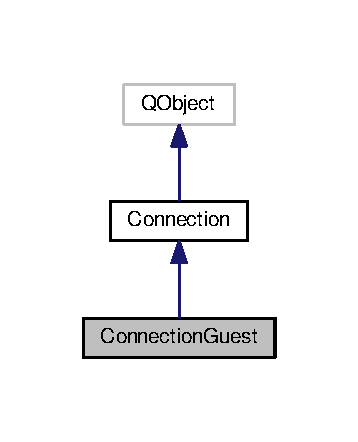
\includegraphics[width=172pt]{classMODEL_1_1ConnectionGuest__inherit__graph}
\end{center}
\end{figure}


Collaboration diagram for Connection\+Guest\+:\nopagebreak
\begin{figure}[H]
\begin{center}
\leavevmode
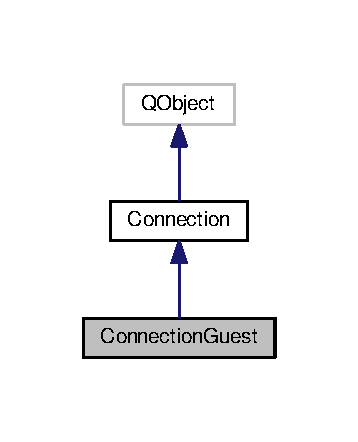
\includegraphics[width=172pt]{classMODEL_1_1ConnectionGuest__coll__graph}
\end{center}
\end{figure}
\subsection*{Public Member Functions}
\begin{DoxyCompactItemize}
\item 
\hyperlink{classMODEL_1_1ConnectionGuest_ab8d5bc0edf4d5533d3c9340d901e8677}{Connection\+Guest} (const std\+::string \&\hyperlink{classMODEL_1_1ConnectionGuest_a8b6f74419f28d6b9d96568f2f1087c3e}{address}, int \hyperlink{classMODEL_1_1ConnectionGuest_a63c89c04d1feae07ca35558055155ffb}{port}, std\+::function$<$ void(const Q\+Byte\+Array \&)$>$ \hyperlink{classMODEL_1_1Connection_aa0b44072225e1b07b646bd973719ac80}{callback\+On\+Data\+Received}, std\+::function$<$ void()$>$ \hyperlink{classMODEL_1_1Connection_a0cb35149e127dbce2a09f0ac5d5cfc16}{callback\+On\+Connected}, Q\+Object $\ast$parent=nullptr)
\item 
\hyperlink{classMODEL_1_1ConnectionGuest_ae5f32ba2fd933170b2652b1b35441e8b}{Connection\+Guest} (\hyperlink{classMODEL_1_1ConnectionGuest}{Connection\+Guest} const \&)=delete
\item 
\hyperlink{classMODEL_1_1ConnectionGuest}{Connection\+Guest} \& \hyperlink{classMODEL_1_1ConnectionGuest_ae55994c212e438a0345319dc2de4fb3a}{operator=} (\hyperlink{classMODEL_1_1ConnectionGuest}{Connection\+Guest} const \&other)=delete
\item 
\hyperlink{classMODEL_1_1ConnectionGuest_a396b57f90e3db3e21334e007590d6991}{Connection\+Guest} (\hyperlink{classMODEL_1_1ConnectionGuest}{Connection\+Guest} \&\&other)=delete
\item 
\hyperlink{classMODEL_1_1ConnectionGuest}{Connection\+Guest} \& \hyperlink{classMODEL_1_1ConnectionGuest_a66b6e88685e8545357fe457d087c0c38}{operator=} (\hyperlink{classMODEL_1_1ConnectionGuest}{Connection\+Guest} \&\&other)=delete
\end{DoxyCompactItemize}
\subsection*{Protected Member Functions}
\begin{DoxyCompactItemize}
\item 
void \hyperlink{classMODEL_1_1ConnectionGuest_ac867d4f9a602bf9d11bf2c653cbf4fe4}{begin\+Connecting} () override
\end{DoxyCompactItemize}
\subsection*{Private Attributes}
\begin{DoxyCompactItemize}
\item 
std\+::string \hyperlink{classMODEL_1_1ConnectionGuest_a8b6f74419f28d6b9d96568f2f1087c3e}{address}
\item 
int \hyperlink{classMODEL_1_1ConnectionGuest_a63c89c04d1feae07ca35558055155ffb}{port}
\end{DoxyCompactItemize}
\subsection*{Additional Inherited Members}


\subsection{Detailed Description}
Inherits from \hyperlink{classMODEL_1_1Connection}{Connection} and implements the functionality for connection used by guest. 

\subsection{Constructor \& Destructor Documentation}
\index{M\+O\+D\+E\+L\+::\+Connection\+Guest@{M\+O\+D\+E\+L\+::\+Connection\+Guest}!Connection\+Guest@{Connection\+Guest}}
\index{Connection\+Guest@{Connection\+Guest}!M\+O\+D\+E\+L\+::\+Connection\+Guest@{M\+O\+D\+E\+L\+::\+Connection\+Guest}}
\subsubsection[{\texorpdfstring{Connection\+Guest(const std\+::string \&address, int port, std\+::function$<$ void(const Q\+Byte\+Array \&)$>$ callback\+On\+Data\+Received, std\+::function$<$ void()$>$ callback\+On\+Connected, Q\+Object $\ast$parent=nullptr)}{ConnectionGuest(const std::string &address, int port, std::function< void(const QByteArray &)> callbackOnDataReceived, std::function< void()> callbackOnConnected, QObject *parent=nullptr)}}]{\setlength{\rightskip}{0pt plus 5cm}{\bf Connection\+Guest} (
\begin{DoxyParamCaption}
\item[{const std\+::string \&}]{address, }
\item[{int}]{port, }
\item[{std\+::function$<$ void(const Q\+Byte\+Array \&)$>$}]{callback\+On\+Data\+Received, }
\item[{std\+::function$<$ void()$>$}]{callback\+On\+Connected, }
\item[{Q\+Object $\ast$}]{parent = {\ttfamily nullptr}}
\end{DoxyParamCaption}
)\hspace{0.3cm}{\ttfamily [explicit]}}\hypertarget{classMODEL_1_1ConnectionGuest_ab8d5bc0edf4d5533d3c9340d901e8677}{}\label{classMODEL_1_1ConnectionGuest_ab8d5bc0edf4d5533d3c9340d901e8677}

\begin{DoxyParams}{Parameters}
{\em callback\+On\+Data\+Received} & called when full data blcock is received. \\
\hline
{\em callback\+On\+Connected} & called when connection is established \\
\hline
\end{DoxyParams}
\index{M\+O\+D\+E\+L\+::\+Connection\+Guest@{M\+O\+D\+E\+L\+::\+Connection\+Guest}!Connection\+Guest@{Connection\+Guest}}
\index{Connection\+Guest@{Connection\+Guest}!M\+O\+D\+E\+L\+::\+Connection\+Guest@{M\+O\+D\+E\+L\+::\+Connection\+Guest}}
\subsubsection[{\texorpdfstring{Connection\+Guest(\+Connection\+Guest const \&)=delete}{ConnectionGuest(ConnectionGuest const &)=delete}}]{\setlength{\rightskip}{0pt plus 5cm}{\bf Connection\+Guest} (
\begin{DoxyParamCaption}
\item[{{\bf Connection\+Guest} const \&}]{}
\end{DoxyParamCaption}
)\hspace{0.3cm}{\ttfamily [delete]}}\hypertarget{classMODEL_1_1ConnectionGuest_ae5f32ba2fd933170b2652b1b35441e8b}{}\label{classMODEL_1_1ConnectionGuest_ae5f32ba2fd933170b2652b1b35441e8b}
\index{M\+O\+D\+E\+L\+::\+Connection\+Guest@{M\+O\+D\+E\+L\+::\+Connection\+Guest}!Connection\+Guest@{Connection\+Guest}}
\index{Connection\+Guest@{Connection\+Guest}!M\+O\+D\+E\+L\+::\+Connection\+Guest@{M\+O\+D\+E\+L\+::\+Connection\+Guest}}
\subsubsection[{\texorpdfstring{Connection\+Guest(\+Connection\+Guest \&\&other)=delete}{ConnectionGuest(ConnectionGuest &&other)=delete}}]{\setlength{\rightskip}{0pt plus 5cm}{\bf Connection\+Guest} (
\begin{DoxyParamCaption}
\item[{{\bf Connection\+Guest} \&\&}]{other}
\end{DoxyParamCaption}
)\hspace{0.3cm}{\ttfamily [delete]}}\hypertarget{classMODEL_1_1ConnectionGuest_a396b57f90e3db3e21334e007590d6991}{}\label{classMODEL_1_1ConnectionGuest_a396b57f90e3db3e21334e007590d6991}


\subsection{Member Function Documentation}
\index{M\+O\+D\+E\+L\+::\+Connection\+Guest@{M\+O\+D\+E\+L\+::\+Connection\+Guest}!begin\+Connecting@{begin\+Connecting}}
\index{begin\+Connecting@{begin\+Connecting}!M\+O\+D\+E\+L\+::\+Connection\+Guest@{M\+O\+D\+E\+L\+::\+Connection\+Guest}}
\subsubsection[{\texorpdfstring{begin\+Connecting() override}{beginConnecting() override}}]{\setlength{\rightskip}{0pt plus 5cm}void begin\+Connecting (
\begin{DoxyParamCaption}
{}
\end{DoxyParamCaption}
)\hspace{0.3cm}{\ttfamily [override]}, {\ttfamily [protected]}, {\ttfamily [virtual]}}\hypertarget{classMODEL_1_1ConnectionGuest_ac867d4f9a602bf9d11bf2c653cbf4fe4}{}\label{classMODEL_1_1ConnectionGuest_ac867d4f9a602bf9d11bf2c653cbf4fe4}


Implements \hyperlink{classMODEL_1_1Connection_ae3e484e0f3217ab38dbaa36f4a379f69}{Connection}.

\index{M\+O\+D\+E\+L\+::\+Connection\+Guest@{M\+O\+D\+E\+L\+::\+Connection\+Guest}!operator=@{operator=}}
\index{operator=@{operator=}!M\+O\+D\+E\+L\+::\+Connection\+Guest@{M\+O\+D\+E\+L\+::\+Connection\+Guest}}
\subsubsection[{\texorpdfstring{operator=(\+Connection\+Guest const \&other)=delete}{operator=(ConnectionGuest const &other)=delete}}]{\setlength{\rightskip}{0pt plus 5cm}{\bf Connection\+Guest}\& operator= (
\begin{DoxyParamCaption}
\item[{{\bf Connection\+Guest} const \&}]{other}
\end{DoxyParamCaption}
)\hspace{0.3cm}{\ttfamily [delete]}}\hypertarget{classMODEL_1_1ConnectionGuest_ae55994c212e438a0345319dc2de4fb3a}{}\label{classMODEL_1_1ConnectionGuest_ae55994c212e438a0345319dc2de4fb3a}
\index{M\+O\+D\+E\+L\+::\+Connection\+Guest@{M\+O\+D\+E\+L\+::\+Connection\+Guest}!operator=@{operator=}}
\index{operator=@{operator=}!M\+O\+D\+E\+L\+::\+Connection\+Guest@{M\+O\+D\+E\+L\+::\+Connection\+Guest}}
\subsubsection[{\texorpdfstring{operator=(\+Connection\+Guest \&\&other)=delete}{operator=(ConnectionGuest &&other)=delete}}]{\setlength{\rightskip}{0pt plus 5cm}{\bf Connection\+Guest}\& operator= (
\begin{DoxyParamCaption}
\item[{{\bf Connection\+Guest} \&\&}]{other}
\end{DoxyParamCaption}
)\hspace{0.3cm}{\ttfamily [delete]}}\hypertarget{classMODEL_1_1ConnectionGuest_a66b6e88685e8545357fe457d087c0c38}{}\label{classMODEL_1_1ConnectionGuest_a66b6e88685e8545357fe457d087c0c38}


\subsection{Member Data Documentation}
\index{M\+O\+D\+E\+L\+::\+Connection\+Guest@{M\+O\+D\+E\+L\+::\+Connection\+Guest}!address@{address}}
\index{address@{address}!M\+O\+D\+E\+L\+::\+Connection\+Guest@{M\+O\+D\+E\+L\+::\+Connection\+Guest}}
\subsubsection[{\texorpdfstring{address}{address}}]{\setlength{\rightskip}{0pt plus 5cm}std\+::string address\hspace{0.3cm}{\ttfamily [private]}}\hypertarget{classMODEL_1_1ConnectionGuest_a8b6f74419f28d6b9d96568f2f1087c3e}{}\label{classMODEL_1_1ConnectionGuest_a8b6f74419f28d6b9d96568f2f1087c3e}
\index{M\+O\+D\+E\+L\+::\+Connection\+Guest@{M\+O\+D\+E\+L\+::\+Connection\+Guest}!port@{port}}
\index{port@{port}!M\+O\+D\+E\+L\+::\+Connection\+Guest@{M\+O\+D\+E\+L\+::\+Connection\+Guest}}
\subsubsection[{\texorpdfstring{port}{port}}]{\setlength{\rightskip}{0pt plus 5cm}int port\hspace{0.3cm}{\ttfamily [private]}}\hypertarget{classMODEL_1_1ConnectionGuest_a63c89c04d1feae07ca35558055155ffb}{}\label{classMODEL_1_1ConnectionGuest_a63c89c04d1feae07ca35558055155ffb}


The documentation for this class was generated from the following files\+:\begin{DoxyCompactItemize}
\item 
model/\hyperlink{connection__guest_8h}{connection\+\_\+guest.\+h}\item 
model/\hyperlink{connection__guest_8cpp}{connection\+\_\+guest.\+cpp}\end{DoxyCompactItemize}

\hypertarget{classMODEL_1_1ConnectionHost}{}\section{Connection\+Host Class Reference}
\label{classMODEL_1_1ConnectionHost}\index{Connection\+Host@{Connection\+Host}}


Inherits from \hyperlink{classMODEL_1_1Connection}{Connection} and implements the functionality for connection used by host.  




{\ttfamily \#include $<$connection\+\_\+host.\+h$>$}



Inheritance diagram for Connection\+Host\+:\nopagebreak
\begin{figure}[H]
\begin{center}
\leavevmode
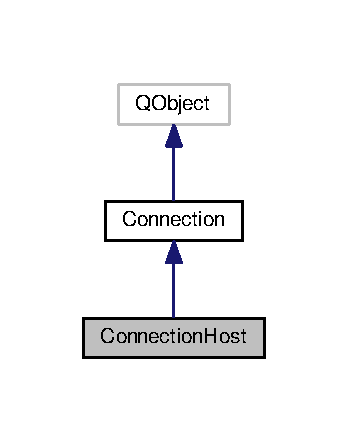
\includegraphics[width=167pt]{classMODEL_1_1ConnectionHost__inherit__graph}
\end{center}
\end{figure}


Collaboration diagram for Connection\+Host\+:\nopagebreak
\begin{figure}[H]
\begin{center}
\leavevmode
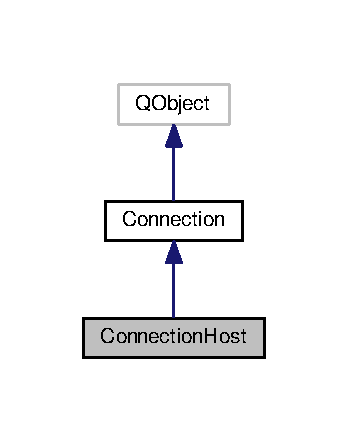
\includegraphics[width=167pt]{classMODEL_1_1ConnectionHost__coll__graph}
\end{center}
\end{figure}
\subsection*{Public Member Functions}
\begin{DoxyCompactItemize}
\item 
\hyperlink{classMODEL_1_1ConnectionHost_aa640c695c3148eaf447b1204c1d6af77}{Connection\+Host} (std\+::function$<$ void(const Q\+Byte\+Array \&)$>$ \hyperlink{classMODEL_1_1Connection_aa0b44072225e1b07b646bd973719ac80}{callback\+On\+Data\+Received}, std\+::function$<$ void()$>$ \hyperlink{classMODEL_1_1Connection_a0cb35149e127dbce2a09f0ac5d5cfc16}{callback\+On\+Connected}, Q\+Object $\ast$parent=nullptr)
\item 
\hyperlink{classMODEL_1_1ConnectionHost_af256b1f5783889ef9b3d78015b98807c}{$\sim$\+Connection\+Host} ()
\item 
\hyperlink{classMODEL_1_1ConnectionHost_aaa81e7db67470298d4282efedbbfd199}{Connection\+Host} (\hyperlink{classMODEL_1_1ConnectionHost}{Connection\+Host} const \&)=delete
\item 
\hyperlink{classMODEL_1_1ConnectionHost}{Connection\+Host} \& \hyperlink{classMODEL_1_1ConnectionHost_a734c9df80c90ccd6acaab9a0d6d2a7f8}{operator=} (\hyperlink{classMODEL_1_1ConnectionHost}{Connection\+Host} const \&other)=delete
\item 
\hyperlink{classMODEL_1_1ConnectionHost_aee554c351828b430390c3227fdd717ea}{Connection\+Host} (\hyperlink{classMODEL_1_1ConnectionHost}{Connection\+Host} \&\&other)=delete
\item 
\hyperlink{classMODEL_1_1ConnectionHost}{Connection\+Host} \& \hyperlink{classMODEL_1_1ConnectionHost_afac3f49bd01c8e0b8236f8a329831bc6}{operator=} (\hyperlink{classMODEL_1_1ConnectionHost}{Connection\+Host} \&\&other)=delete
\end{DoxyCompactItemize}
\subsection*{Protected Member Functions}
\begin{DoxyCompactItemize}
\item 
void \hyperlink{classMODEL_1_1ConnectionHost_ac867d4f9a602bf9d11bf2c653cbf4fe4}{begin\+Connecting} () override
\end{DoxyCompactItemize}
\subsection*{Private Attributes}
\begin{DoxyCompactItemize}
\item 
Q\+Tcp\+Server $\ast$ \hyperlink{classMODEL_1_1ConnectionHost_a79c9047a78bc919910a66376a7c5bb4d}{tcp\+Server} \{nullptr\}
\end{DoxyCompactItemize}
\subsection*{Additional Inherited Members}


\subsection{Detailed Description}
Inherits from \hyperlink{classMODEL_1_1Connection}{Connection} and implements the functionality for connection used by host. 

\subsection{Constructor \& Destructor Documentation}
\index{M\+O\+D\+E\+L\+::\+Connection\+Host@{M\+O\+D\+E\+L\+::\+Connection\+Host}!Connection\+Host@{Connection\+Host}}
\index{Connection\+Host@{Connection\+Host}!M\+O\+D\+E\+L\+::\+Connection\+Host@{M\+O\+D\+E\+L\+::\+Connection\+Host}}
\subsubsection[{\texorpdfstring{Connection\+Host(std\+::function$<$ void(const Q\+Byte\+Array \&)$>$ callback\+On\+Data\+Received, std\+::function$<$ void()$>$ callback\+On\+Connected, Q\+Object $\ast$parent=nullptr)}{ConnectionHost(std::function< void(const QByteArray &)> callbackOnDataReceived, std::function< void()> callbackOnConnected, QObject *parent=nullptr)}}]{\setlength{\rightskip}{0pt plus 5cm}{\bf Connection\+Host} (
\begin{DoxyParamCaption}
\item[{std\+::function$<$ void(const Q\+Byte\+Array \&)$>$}]{callback\+On\+Data\+Received, }
\item[{std\+::function$<$ void()$>$}]{callback\+On\+Connected, }
\item[{Q\+Object $\ast$}]{parent = {\ttfamily nullptr}}
\end{DoxyParamCaption}
)\hspace{0.3cm}{\ttfamily [explicit]}}\hypertarget{classMODEL_1_1ConnectionHost_aa640c695c3148eaf447b1204c1d6af77}{}\label{classMODEL_1_1ConnectionHost_aa640c695c3148eaf447b1204c1d6af77}

\begin{DoxyParams}{Parameters}
{\em callback\+On\+Data\+Received} & called when full data blcock is received. \\
\hline
{\em callback\+On\+Connected} & called when connection is established \\
\hline
\end{DoxyParams}
\index{M\+O\+D\+E\+L\+::\+Connection\+Host@{M\+O\+D\+E\+L\+::\+Connection\+Host}!````~Connection\+Host@{$\sim$\+Connection\+Host}}
\index{````~Connection\+Host@{$\sim$\+Connection\+Host}!M\+O\+D\+E\+L\+::\+Connection\+Host@{M\+O\+D\+E\+L\+::\+Connection\+Host}}
\subsubsection[{\texorpdfstring{$\sim$\+Connection\+Host()}{~ConnectionHost()}}]{\setlength{\rightskip}{0pt plus 5cm}$\sim${\bf Connection\+Host} (
\begin{DoxyParamCaption}
{}
\end{DoxyParamCaption}
)}\hypertarget{classMODEL_1_1ConnectionHost_af256b1f5783889ef9b3d78015b98807c}{}\label{classMODEL_1_1ConnectionHost_af256b1f5783889ef9b3d78015b98807c}
\index{M\+O\+D\+E\+L\+::\+Connection\+Host@{M\+O\+D\+E\+L\+::\+Connection\+Host}!Connection\+Host@{Connection\+Host}}
\index{Connection\+Host@{Connection\+Host}!M\+O\+D\+E\+L\+::\+Connection\+Host@{M\+O\+D\+E\+L\+::\+Connection\+Host}}
\subsubsection[{\texorpdfstring{Connection\+Host(\+Connection\+Host const \&)=delete}{ConnectionHost(ConnectionHost const &)=delete}}]{\setlength{\rightskip}{0pt plus 5cm}{\bf Connection\+Host} (
\begin{DoxyParamCaption}
\item[{{\bf Connection\+Host} const \&}]{}
\end{DoxyParamCaption}
)\hspace{0.3cm}{\ttfamily [delete]}}\hypertarget{classMODEL_1_1ConnectionHost_aaa81e7db67470298d4282efedbbfd199}{}\label{classMODEL_1_1ConnectionHost_aaa81e7db67470298d4282efedbbfd199}
\index{M\+O\+D\+E\+L\+::\+Connection\+Host@{M\+O\+D\+E\+L\+::\+Connection\+Host}!Connection\+Host@{Connection\+Host}}
\index{Connection\+Host@{Connection\+Host}!M\+O\+D\+E\+L\+::\+Connection\+Host@{M\+O\+D\+E\+L\+::\+Connection\+Host}}
\subsubsection[{\texorpdfstring{Connection\+Host(\+Connection\+Host \&\&other)=delete}{ConnectionHost(ConnectionHost &&other)=delete}}]{\setlength{\rightskip}{0pt plus 5cm}{\bf Connection\+Host} (
\begin{DoxyParamCaption}
\item[{{\bf Connection\+Host} \&\&}]{other}
\end{DoxyParamCaption}
)\hspace{0.3cm}{\ttfamily [delete]}}\hypertarget{classMODEL_1_1ConnectionHost_aee554c351828b430390c3227fdd717ea}{}\label{classMODEL_1_1ConnectionHost_aee554c351828b430390c3227fdd717ea}


\subsection{Member Function Documentation}
\index{M\+O\+D\+E\+L\+::\+Connection\+Host@{M\+O\+D\+E\+L\+::\+Connection\+Host}!begin\+Connecting@{begin\+Connecting}}
\index{begin\+Connecting@{begin\+Connecting}!M\+O\+D\+E\+L\+::\+Connection\+Host@{M\+O\+D\+E\+L\+::\+Connection\+Host}}
\subsubsection[{\texorpdfstring{begin\+Connecting() override}{beginConnecting() override}}]{\setlength{\rightskip}{0pt plus 5cm}void begin\+Connecting (
\begin{DoxyParamCaption}
{}
\end{DoxyParamCaption}
)\hspace{0.3cm}{\ttfamily [override]}, {\ttfamily [protected]}, {\ttfamily [virtual]}}\hypertarget{classMODEL_1_1ConnectionHost_ac867d4f9a602bf9d11bf2c653cbf4fe4}{}\label{classMODEL_1_1ConnectionHost_ac867d4f9a602bf9d11bf2c653cbf4fe4}


Implements \hyperlink{classMODEL_1_1Connection_ae3e484e0f3217ab38dbaa36f4a379f69}{Connection}.

\index{M\+O\+D\+E\+L\+::\+Connection\+Host@{M\+O\+D\+E\+L\+::\+Connection\+Host}!operator=@{operator=}}
\index{operator=@{operator=}!M\+O\+D\+E\+L\+::\+Connection\+Host@{M\+O\+D\+E\+L\+::\+Connection\+Host}}
\subsubsection[{\texorpdfstring{operator=(\+Connection\+Host const \&other)=delete}{operator=(ConnectionHost const &other)=delete}}]{\setlength{\rightskip}{0pt plus 5cm}{\bf Connection\+Host}\& operator= (
\begin{DoxyParamCaption}
\item[{{\bf Connection\+Host} const \&}]{other}
\end{DoxyParamCaption}
)\hspace{0.3cm}{\ttfamily [delete]}}\hypertarget{classMODEL_1_1ConnectionHost_a734c9df80c90ccd6acaab9a0d6d2a7f8}{}\label{classMODEL_1_1ConnectionHost_a734c9df80c90ccd6acaab9a0d6d2a7f8}
\index{M\+O\+D\+E\+L\+::\+Connection\+Host@{M\+O\+D\+E\+L\+::\+Connection\+Host}!operator=@{operator=}}
\index{operator=@{operator=}!M\+O\+D\+E\+L\+::\+Connection\+Host@{M\+O\+D\+E\+L\+::\+Connection\+Host}}
\subsubsection[{\texorpdfstring{operator=(\+Connection\+Host \&\&other)=delete}{operator=(ConnectionHost &&other)=delete}}]{\setlength{\rightskip}{0pt plus 5cm}{\bf Connection\+Host}\& operator= (
\begin{DoxyParamCaption}
\item[{{\bf Connection\+Host} \&\&}]{other}
\end{DoxyParamCaption}
)\hspace{0.3cm}{\ttfamily [delete]}}\hypertarget{classMODEL_1_1ConnectionHost_afac3f49bd01c8e0b8236f8a329831bc6}{}\label{classMODEL_1_1ConnectionHost_afac3f49bd01c8e0b8236f8a329831bc6}


\subsection{Member Data Documentation}
\index{M\+O\+D\+E\+L\+::\+Connection\+Host@{M\+O\+D\+E\+L\+::\+Connection\+Host}!tcp\+Server@{tcp\+Server}}
\index{tcp\+Server@{tcp\+Server}!M\+O\+D\+E\+L\+::\+Connection\+Host@{M\+O\+D\+E\+L\+::\+Connection\+Host}}
\subsubsection[{\texorpdfstring{tcp\+Server}{tcpServer}}]{\setlength{\rightskip}{0pt plus 5cm}Q\+Tcp\+Server$\ast$ tcp\+Server \{nullptr\}\hspace{0.3cm}{\ttfamily [private]}}\hypertarget{classMODEL_1_1ConnectionHost_a79c9047a78bc919910a66376a7c5bb4d}{}\label{classMODEL_1_1ConnectionHost_a79c9047a78bc919910a66376a7c5bb4d}


The documentation for this class was generated from the following files\+:\begin{DoxyCompactItemize}
\item 
model/\hyperlink{connection__host_8h}{connection\+\_\+host.\+h}\item 
model/\hyperlink{connection__host_8cpp}{connection\+\_\+host.\+cpp}\end{DoxyCompactItemize}

\hypertarget{classConnectionTest}{}\section{Connection\+Test Class Reference}
\label{classConnectionTest}\index{Connection\+Test@{Connection\+Test}}


Inheritance diagram for Connection\+Test\+:\nopagebreak
\begin{figure}[H]
\begin{center}
\leavevmode
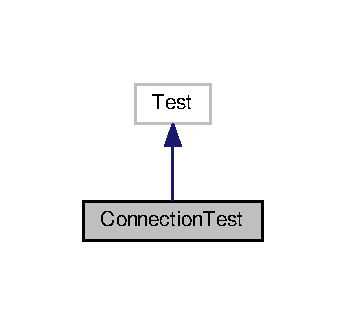
\includegraphics[width=166pt]{classConnectionTest__inherit__graph}
\end{center}
\end{figure}


Collaboration diagram for Connection\+Test\+:\nopagebreak
\begin{figure}[H]
\begin{center}
\leavevmode
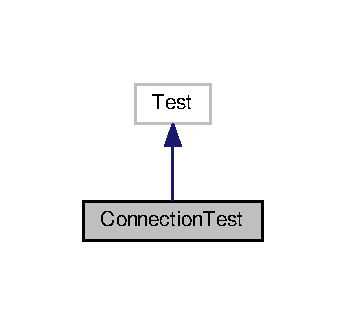
\includegraphics[width=166pt]{classConnectionTest__coll__graph}
\end{center}
\end{figure}
\subsection*{Protected Member Functions}
\begin{DoxyCompactItemize}
\item 
\hyperlink{classConnectionTest_a233bb6627cf350eb31558b00a1e8ad18}{Connection\+Test} ()
\item 
virtual \hyperlink{classConnectionTest_a3d1ab239eb1255da806e8b029ccce335}{$\sim$\+Connection\+Test} ()
\item 
virtual void \hyperlink{classConnectionTest_a901706a587f9ae84df8b2395fbe759cb}{Set\+Up} ()
\item 
virtual void \hyperlink{classConnectionTest_a870a092058305911f3d42df45dd657e5}{Tear\+Down} ()
\end{DoxyCompactItemize}


\subsection{Constructor \& Destructor Documentation}
\index{Connection\+Test@{Connection\+Test}!Connection\+Test@{Connection\+Test}}
\index{Connection\+Test@{Connection\+Test}!Connection\+Test@{Connection\+Test}}
\subsubsection[{\texorpdfstring{Connection\+Test()}{ConnectionTest()}}]{\setlength{\rightskip}{0pt plus 5cm}{\bf Connection\+Test} (
\begin{DoxyParamCaption}
{}
\end{DoxyParamCaption}
)\hspace{0.3cm}{\ttfamily [inline]}, {\ttfamily [protected]}}\hypertarget{classConnectionTest_a233bb6627cf350eb31558b00a1e8ad18}{}\label{classConnectionTest_a233bb6627cf350eb31558b00a1e8ad18}
\index{Connection\+Test@{Connection\+Test}!````~Connection\+Test@{$\sim$\+Connection\+Test}}
\index{````~Connection\+Test@{$\sim$\+Connection\+Test}!Connection\+Test@{Connection\+Test}}
\subsubsection[{\texorpdfstring{$\sim$\+Connection\+Test()}{~ConnectionTest()}}]{\setlength{\rightskip}{0pt plus 5cm}virtual $\sim${\bf Connection\+Test} (
\begin{DoxyParamCaption}
{}
\end{DoxyParamCaption}
)\hspace{0.3cm}{\ttfamily [inline]}, {\ttfamily [protected]}, {\ttfamily [virtual]}}\hypertarget{classConnectionTest_a3d1ab239eb1255da806e8b029ccce335}{}\label{classConnectionTest_a3d1ab239eb1255da806e8b029ccce335}


\subsection{Member Function Documentation}
\index{Connection\+Test@{Connection\+Test}!Set\+Up@{Set\+Up}}
\index{Set\+Up@{Set\+Up}!Connection\+Test@{Connection\+Test}}
\subsubsection[{\texorpdfstring{Set\+Up()}{SetUp()}}]{\setlength{\rightskip}{0pt plus 5cm}virtual void Set\+Up (
\begin{DoxyParamCaption}
{}
\end{DoxyParamCaption}
)\hspace{0.3cm}{\ttfamily [inline]}, {\ttfamily [protected]}, {\ttfamily [virtual]}}\hypertarget{classConnectionTest_a901706a587f9ae84df8b2395fbe759cb}{}\label{classConnectionTest_a901706a587f9ae84df8b2395fbe759cb}
\index{Connection\+Test@{Connection\+Test}!Tear\+Down@{Tear\+Down}}
\index{Tear\+Down@{Tear\+Down}!Connection\+Test@{Connection\+Test}}
\subsubsection[{\texorpdfstring{Tear\+Down()}{TearDown()}}]{\setlength{\rightskip}{0pt plus 5cm}virtual void Tear\+Down (
\begin{DoxyParamCaption}
{}
\end{DoxyParamCaption}
)\hspace{0.3cm}{\ttfamily [inline]}, {\ttfamily [protected]}, {\ttfamily [virtual]}}\hypertarget{classConnectionTest_a870a092058305911f3d42df45dd657e5}{}\label{classConnectionTest_a870a092058305911f3d42df45dd657e5}


The documentation for this class was generated from the following file\+:\begin{DoxyCompactItemize}
\item 
\hyperlink{test__connection_8cpp}{test\+\_\+connection.\+cpp}\end{DoxyCompactItemize}

\hypertarget{classControllerInterface}{}\section{Controller\+Interface Class Reference}
\label{classControllerInterface}\index{Controller\+Interface@{Controller\+Interface}}


The base class that defines the controller interface.  




{\ttfamily \#include $<$controller\+\_\+interface.\+h$>$}



Inheritance diagram for Controller\+Interface\+:\nopagebreak
\begin{figure}[H]
\begin{center}
\leavevmode
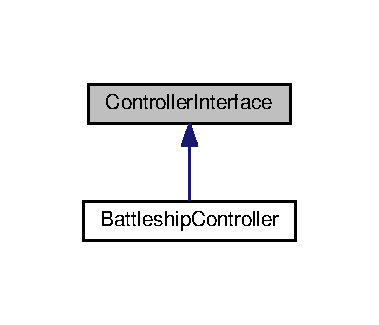
\includegraphics[width=182pt]{classControllerInterface__inherit__graph}
\end{center}
\end{figure}
\subsection*{Public Member Functions}
\begin{DoxyCompactItemize}
\item 
virtual \hyperlink{classControllerInterface_a46df3c69ef790fee7dc8c58235dc689f}{$\sim$\+Controller\+Interface} ()
\item 
virtual void \hyperlink{classControllerInterface_a0a1077ca83efdd21ffe8b1c042eb9b3b}{start\+New\+Game\+As\+Host} (const Q\+String \&player\+Name, const Q\+String \&age)=0
\item 
virtual void \hyperlink{classControllerInterface_a59fe7601f2d7853043c7056d892b86a4}{start\+New\+Game\+As\+Guest} (const Q\+String \&address, const Q\+String \&port, const Q\+String \&player\+Name, const Q\+String \&age)=0
\end{DoxyCompactItemize}


\subsection{Detailed Description}
The base class that defines the controller interface. 

\subsection{Constructor \& Destructor Documentation}
\index{Controller\+Interface@{Controller\+Interface}!````~Controller\+Interface@{$\sim$\+Controller\+Interface}}
\index{````~Controller\+Interface@{$\sim$\+Controller\+Interface}!Controller\+Interface@{Controller\+Interface}}
\subsubsection[{\texorpdfstring{$\sim$\+Controller\+Interface()}{~ControllerInterface()}}]{\setlength{\rightskip}{0pt plus 5cm}virtual $\sim${\bf Controller\+Interface} (
\begin{DoxyParamCaption}
{}
\end{DoxyParamCaption}
)\hspace{0.3cm}{\ttfamily [inline]}, {\ttfamily [virtual]}}\hypertarget{classControllerInterface_a46df3c69ef790fee7dc8c58235dc689f}{}\label{classControllerInterface_a46df3c69ef790fee7dc8c58235dc689f}


\subsection{Member Function Documentation}
\index{Controller\+Interface@{Controller\+Interface}!start\+New\+Game\+As\+Guest@{start\+New\+Game\+As\+Guest}}
\index{start\+New\+Game\+As\+Guest@{start\+New\+Game\+As\+Guest}!Controller\+Interface@{Controller\+Interface}}
\subsubsection[{\texorpdfstring{start\+New\+Game\+As\+Guest(const Q\+String \&address, const Q\+String \&port, const Q\+String \&player\+Name, const Q\+String \&age)=0}{startNewGameAsGuest(const QString &address, const QString &port, const QString &playerName, const QString &age)=0}}]{\setlength{\rightskip}{0pt plus 5cm}virtual void start\+New\+Game\+As\+Guest (
\begin{DoxyParamCaption}
\item[{const Q\+String \&}]{address, }
\item[{const Q\+String \&}]{port, }
\item[{const Q\+String \&}]{player\+Name, }
\item[{const Q\+String \&}]{age}
\end{DoxyParamCaption}
)\hspace{0.3cm}{\ttfamily [pure virtual]}}\hypertarget{classControllerInterface_a59fe7601f2d7853043c7056d892b86a4}{}\label{classControllerInterface_a59fe7601f2d7853043c7056d892b86a4}
connect to a host as a guest over the network 

Implemented in \hyperlink{classBattleshipController_a97013c1a4017c85bcc654424208a0cb4}{Battleship\+Controller}.

\index{Controller\+Interface@{Controller\+Interface}!start\+New\+Game\+As\+Host@{start\+New\+Game\+As\+Host}}
\index{start\+New\+Game\+As\+Host@{start\+New\+Game\+As\+Host}!Controller\+Interface@{Controller\+Interface}}
\subsubsection[{\texorpdfstring{start\+New\+Game\+As\+Host(const Q\+String \&player\+Name, const Q\+String \&age)=0}{startNewGameAsHost(const QString &playerName, const QString &age)=0}}]{\setlength{\rightskip}{0pt plus 5cm}virtual void start\+New\+Game\+As\+Host (
\begin{DoxyParamCaption}
\item[{const Q\+String \&}]{player\+Name, }
\item[{const Q\+String \&}]{age}
\end{DoxyParamCaption}
)\hspace{0.3cm}{\ttfamily [pure virtual]}}\hypertarget{classControllerInterface_a0a1077ca83efdd21ffe8b1c042eb9b3b}{}\label{classControllerInterface_a0a1077ca83efdd21ffe8b1c042eb9b3b}
begin new game as host over the network. But first wat for guest to join. 

Implemented in \hyperlink{classBattleshipController_a37949c2d70eb648a5957f9e60e86085c}{Battleship\+Controller}.



The documentation for this class was generated from the following file\+:\begin{DoxyCompactItemize}
\item 
common/\hyperlink{controller__interface_8h}{controller\+\_\+interface.\+h}\end{DoxyCompactItemize}

\hypertarget{classGUI_1_1CoordinateSystem}{}\section{Coordinate\+System Class Reference}
\label{classGUI_1_1CoordinateSystem}\index{Coordinate\+System@{Coordinate\+System}}


A virtual base class that defines the essential data for all coordinate systems.  




{\ttfamily \#include $<$coordinatesystem.\+h$>$}



Inheritance diagram for Coordinate\+System\+:\nopagebreak
\begin{figure}[H]
\begin{center}
\leavevmode
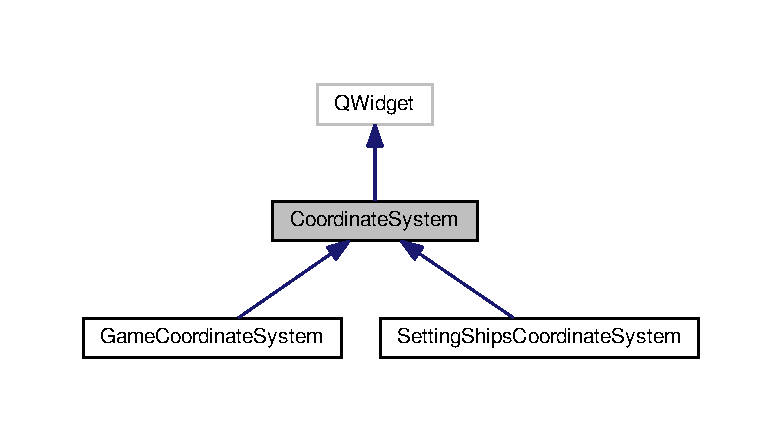
\includegraphics[width=350pt]{classGUI_1_1CoordinateSystem__inherit__graph}
\end{center}
\end{figure}


Collaboration diagram for Coordinate\+System\+:\nopagebreak
\begin{figure}[H]
\begin{center}
\leavevmode
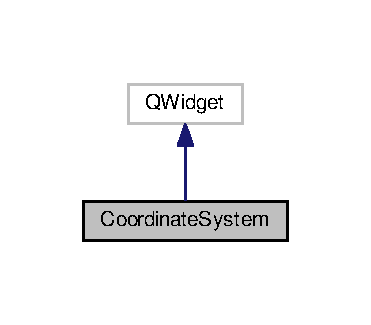
\includegraphics[width=178pt]{classGUI_1_1CoordinateSystem__coll__graph}
\end{center}
\end{figure}
\subsection*{Public Member Functions}
\begin{DoxyCompactItemize}
\item 
\hyperlink{classGUI_1_1CoordinateSystem_a279a1ccd5bfc8d71d086cb2d7fb77ec3}{Coordinate\+System} (Q\+Widget $\ast$\hyperlink{classGUI_1_1CoordinateSystem_a1799d742cabf4aedc2b3553023ccd368}{parent}=nullptr)
\item 
\hyperlink{classGUI_1_1CoordinateSystem_a6b68547f4cdb1b9a42b0e31fe61c3064}{$\sim$\+Coordinate\+System} ()
\item 
void \hyperlink{classGUI_1_1CoordinateSystem_a457f85ceb4ade790e815a0ea27e7760e}{paint\+Text} ()
\begin{DoxyCompactList}\small\item\em zeichnet die Beschriftungen der X-\/ und Y-\/\+Achse \end{DoxyCompactList}\item 
void \hyperlink{classGUI_1_1CoordinateSystem_ae1362a28cae5c9ba80e89b7a0734bf0b}{paint\+Axis} ()
\begin{DoxyCompactList}\small\item\em zeichnet die X-\/ und Y-\/\+Achse \end{DoxyCompactList}\item 
void \hyperlink{classGUI_1_1CoordinateSystem_a0abd1bd78d11330c8c70f9eaeec33c2f}{paint\+Ships} ()
\begin{DoxyCompactList}\small\item\em zeichnet die Schiffe aus ships \end{DoxyCompactList}\item 
virtual void \hyperlink{classGUI_1_1CoordinateSystem_a3d41bd83deb883b8d0c8d192bd0b1ddd}{clear\+Field} ()=0
\begin{DoxyCompactList}\small\item\em Eine Funktion, die pure virtual ist, wird fuer eine abstrakte Klasse benoetigt. \end{DoxyCompactList}\item 
Q\+Point \hyperlink{classGUI_1_1CoordinateSystem_a99abd61b7c05252962b38933538410a4}{get\+Coordinates} (int x, int y)
\begin{DoxyCompactList}\small\item\em Rechnet die Pixel-\/\+Koordinaten eines Q\+Point in der \hyperlink{namespaceGUI}{G\+UI} in die mathematisch richtige Werte um und gibt sie zurueck. \end{DoxyCompactList}\end{DoxyCompactItemize}
\subsection*{Public Attributes}
\begin{DoxyCompactItemize}
\item 
std\+::vector$<$ Q\+Line $>$ \hyperlink{classGUI_1_1CoordinateSystem_aace79121ea432bad20264eafaec2e60f}{ships}
\begin{DoxyCompactList}\small\item\em Schiffe. \end{DoxyCompactList}\item 
Q\+Pixmap $\ast$ \hyperlink{classGUI_1_1CoordinateSystem_a4e0ef07bc83595ef2208e719435b2bdb}{target\+\_\+pixmap}
\begin{DoxyCompactList}\small\item\em Pain Device fuer das Koordinatensystem. \end{DoxyCompactList}\item 
Qt\+::\+Global\+Color \hyperlink{classGUI_1_1CoordinateSystem_a10cc8a23e9d2e122f5160ac6cc8c024a}{lines\+\_\+color} = Qt\+::gray
\begin{DoxyCompactList}\small\item\em Farben. \end{DoxyCompactList}\item 
Qt\+::\+Global\+Color \hyperlink{classGUI_1_1CoordinateSystem_a105b11a9cc588b3a0b7c6208b270d5c9}{x\+\_\+y\+\_\+axis\+\_\+color} = Qt\+::black
\item 
Qt\+::\+Global\+Color \hyperlink{classGUI_1_1CoordinateSystem_aade80ae99e4ee3610c175da220484c30}{ships\+\_\+color} = Qt\+::blue
\item 
Qt\+::\+Global\+Color \hyperlink{classGUI_1_1CoordinateSystem_a8263857bd70758bdb9272b15dc87f55f}{bg\+\_\+color} = Qt\+::white
\end{DoxyCompactItemize}
\subsection*{Protected Attributes}
\begin{DoxyCompactItemize}
\item 
Q\+Widget $\ast$ \hyperlink{classGUI_1_1CoordinateSystem_a1799d742cabf4aedc2b3553023ccd368}{parent}
\item 
std\+::vector$<$ Q\+Point $>$ \hyperlink{classGUI_1_1CoordinateSystem_af6b75c3f51fa26c16961a577565e177e}{points}
\begin{DoxyCompactList}\small\item\em Alle Schnittpunkte der Linien auf dem Koordinatensystem. \end{DoxyCompactList}\item 
int \hyperlink{classGUI_1_1CoordinateSystem_af95e9c45410ea5d7085675933c5eeae3}{gamearea} = 400
\item 
int \hyperlink{classGUI_1_1CoordinateSystem_ad513b38928d1200efd7c23313bf19a6f}{space\+\_\+to\+\_\+next\+\_\+line} = 20
\item 
int \hyperlink{classGUI_1_1CoordinateSystem_aee01da46fa67198ecaa2f6f4d640c4be}{ship\+\_\+length} = (\hyperlink{classGUI_1_1CoordinateSystem_af95e9c45410ea5d7085675933c5eeae3}{gamearea}/\hyperlink{classGUI_1_1CoordinateSystem_ad513b38928d1200efd7c23313bf19a6f}{space\+\_\+to\+\_\+next\+\_\+line})$\ast$2
\item 
int \hyperlink{classGUI_1_1CoordinateSystem_a4aea6960b7b2ff7fe72c11feaead9d78}{initial\+\_\+x} = -\/1
\begin{DoxyCompactList}\small\item\em die Ausgangskoordinaten \end{DoxyCompactList}\item 
int \hyperlink{classGUI_1_1CoordinateSystem_a5a8fb7f950cc366b0a248a04fb2270da}{initial\+\_\+y} = -\/1
\item 
int \hyperlink{classGUI_1_1CoordinateSystem_a5e3c4d4ddb249df69bacc54748304113}{final\+\_\+x} = -\/1
\begin{DoxyCompactList}\small\item\em die Endkoordinaten \end{DoxyCompactList}\item 
int \hyperlink{classGUI_1_1CoordinateSystem_a7be498e5c36f146dc15c99d79a1dec26}{final\+\_\+y} = -\/1
\item 
bool \hyperlink{classGUI_1_1CoordinateSystem_a76fde535d6e6d8b00594daf38372fa0d}{mouse\+\_\+pressed} = false
\begin{DoxyCompactList}\small\item\em wird beim mouse\+Press\+Event auf true gesetzt \end{DoxyCompactList}\item 
int \hyperlink{classGUI_1_1CoordinateSystem_aac44d9cfd174bff52e3126dcc059d851}{triangle\+\_\+size} = 5
\begin{DoxyCompactList}\small\item\em bestimmt die Groesse der Pfeile an den Achsen des Koordinatensystems \end{DoxyCompactList}\end{DoxyCompactItemize}


\subsection{Detailed Description}
A virtual base class that defines the essential data for all coordinate systems. 

\subsection{Constructor \& Destructor Documentation}
\index{G\+U\+I\+::\+Coordinate\+System@{G\+U\+I\+::\+Coordinate\+System}!Coordinate\+System@{Coordinate\+System}}
\index{Coordinate\+System@{Coordinate\+System}!G\+U\+I\+::\+Coordinate\+System@{G\+U\+I\+::\+Coordinate\+System}}
\subsubsection[{\texorpdfstring{Coordinate\+System(\+Q\+Widget $\ast$parent=nullptr)}{CoordinateSystem(QWidget *parent=nullptr)}}]{\setlength{\rightskip}{0pt plus 5cm}{\bf Coordinate\+System} (
\begin{DoxyParamCaption}
\item[{Q\+Widget $\ast$}]{parent = {\ttfamily nullptr}}
\end{DoxyParamCaption}
)\hspace{0.3cm}{\ttfamily [explicit]}}\hypertarget{classGUI_1_1CoordinateSystem_a279a1ccd5bfc8d71d086cb2d7fb77ec3}{}\label{classGUI_1_1CoordinateSystem_a279a1ccd5bfc8d71d086cb2d7fb77ec3}
\index{G\+U\+I\+::\+Coordinate\+System@{G\+U\+I\+::\+Coordinate\+System}!````~Coordinate\+System@{$\sim$\+Coordinate\+System}}
\index{````~Coordinate\+System@{$\sim$\+Coordinate\+System}!G\+U\+I\+::\+Coordinate\+System@{G\+U\+I\+::\+Coordinate\+System}}
\subsubsection[{\texorpdfstring{$\sim$\+Coordinate\+System()}{~CoordinateSystem()}}]{\setlength{\rightskip}{0pt plus 5cm}$\sim${\bf Coordinate\+System} (
\begin{DoxyParamCaption}
{}
\end{DoxyParamCaption}
)}\hypertarget{classGUI_1_1CoordinateSystem_a6b68547f4cdb1b9a42b0e31fe61c3064}{}\label{classGUI_1_1CoordinateSystem_a6b68547f4cdb1b9a42b0e31fe61c3064}


\subsection{Member Function Documentation}
\index{G\+U\+I\+::\+Coordinate\+System@{G\+U\+I\+::\+Coordinate\+System}!clear\+Field@{clear\+Field}}
\index{clear\+Field@{clear\+Field}!G\+U\+I\+::\+Coordinate\+System@{G\+U\+I\+::\+Coordinate\+System}}
\subsubsection[{\texorpdfstring{clear\+Field()=0}{clearField()=0}}]{\setlength{\rightskip}{0pt plus 5cm}virtual void clear\+Field (
\begin{DoxyParamCaption}
{}
\end{DoxyParamCaption}
)\hspace{0.3cm}{\ttfamily [pure virtual]}}\hypertarget{classGUI_1_1CoordinateSystem_a3d41bd83deb883b8d0c8d192bd0b1ddd}{}\label{classGUI_1_1CoordinateSystem_a3d41bd83deb883b8d0c8d192bd0b1ddd}


Eine Funktion, die pure virtual ist, wird fuer eine abstrakte Klasse benoetigt. 



Implemented in \hyperlink{classGUI_1_1SettingShipsCoordinateSystem_afcf62685a11ce5529786cc14ddecc7f2}{Setting\+Ships\+Coordinate\+System}, and \hyperlink{classGUI_1_1GameCoordinateSystem_afcf62685a11ce5529786cc14ddecc7f2}{Game\+Coordinate\+System}.

\index{G\+U\+I\+::\+Coordinate\+System@{G\+U\+I\+::\+Coordinate\+System}!get\+Coordinates@{get\+Coordinates}}
\index{get\+Coordinates@{get\+Coordinates}!G\+U\+I\+::\+Coordinate\+System@{G\+U\+I\+::\+Coordinate\+System}}
\subsubsection[{\texorpdfstring{get\+Coordinates(int x, int y)}{getCoordinates(int x, int y)}}]{\setlength{\rightskip}{0pt plus 5cm}Q\+Point get\+Coordinates (
\begin{DoxyParamCaption}
\item[{int}]{x, }
\item[{int}]{y}
\end{DoxyParamCaption}
)}\hypertarget{classGUI_1_1CoordinateSystem_a99abd61b7c05252962b38933538410a4}{}\label{classGUI_1_1CoordinateSystem_a99abd61b7c05252962b38933538410a4}


Rechnet die Pixel-\/\+Koordinaten eines Q\+Point in der \hyperlink{namespaceGUI}{G\+UI} in die mathematisch richtige Werte um und gibt sie zurueck. 

\index{G\+U\+I\+::\+Coordinate\+System@{G\+U\+I\+::\+Coordinate\+System}!paint\+Axis@{paint\+Axis}}
\index{paint\+Axis@{paint\+Axis}!G\+U\+I\+::\+Coordinate\+System@{G\+U\+I\+::\+Coordinate\+System}}
\subsubsection[{\texorpdfstring{paint\+Axis()}{paintAxis()}}]{\setlength{\rightskip}{0pt plus 5cm}void paint\+Axis (
\begin{DoxyParamCaption}
{}
\end{DoxyParamCaption}
)}\hypertarget{classGUI_1_1CoordinateSystem_ae1362a28cae5c9ba80e89b7a0734bf0b}{}\label{classGUI_1_1CoordinateSystem_ae1362a28cae5c9ba80e89b7a0734bf0b}


zeichnet die X-\/ und Y-\/\+Achse 

\index{G\+U\+I\+::\+Coordinate\+System@{G\+U\+I\+::\+Coordinate\+System}!paint\+Ships@{paint\+Ships}}
\index{paint\+Ships@{paint\+Ships}!G\+U\+I\+::\+Coordinate\+System@{G\+U\+I\+::\+Coordinate\+System}}
\subsubsection[{\texorpdfstring{paint\+Ships()}{paintShips()}}]{\setlength{\rightskip}{0pt plus 5cm}void paint\+Ships (
\begin{DoxyParamCaption}
{}
\end{DoxyParamCaption}
)}\hypertarget{classGUI_1_1CoordinateSystem_a0abd1bd78d11330c8c70f9eaeec33c2f}{}\label{classGUI_1_1CoordinateSystem_a0abd1bd78d11330c8c70f9eaeec33c2f}


zeichnet die Schiffe aus ships 

\index{G\+U\+I\+::\+Coordinate\+System@{G\+U\+I\+::\+Coordinate\+System}!paint\+Text@{paint\+Text}}
\index{paint\+Text@{paint\+Text}!G\+U\+I\+::\+Coordinate\+System@{G\+U\+I\+::\+Coordinate\+System}}
\subsubsection[{\texorpdfstring{paint\+Text()}{paintText()}}]{\setlength{\rightskip}{0pt plus 5cm}void paint\+Text (
\begin{DoxyParamCaption}
{}
\end{DoxyParamCaption}
)}\hypertarget{classGUI_1_1CoordinateSystem_a457f85ceb4ade790e815a0ea27e7760e}{}\label{classGUI_1_1CoordinateSystem_a457f85ceb4ade790e815a0ea27e7760e}


zeichnet die Beschriftungen der X-\/ und Y-\/\+Achse 



\subsection{Member Data Documentation}
\index{G\+U\+I\+::\+Coordinate\+System@{G\+U\+I\+::\+Coordinate\+System}!bg\+\_\+color@{bg\+\_\+color}}
\index{bg\+\_\+color@{bg\+\_\+color}!G\+U\+I\+::\+Coordinate\+System@{G\+U\+I\+::\+Coordinate\+System}}
\subsubsection[{\texorpdfstring{bg\+\_\+color}{bg_color}}]{\setlength{\rightskip}{0pt plus 5cm}Qt\+::\+Global\+Color bg\+\_\+color = Qt\+::white}\hypertarget{classGUI_1_1CoordinateSystem_a8263857bd70758bdb9272b15dc87f55f}{}\label{classGUI_1_1CoordinateSystem_a8263857bd70758bdb9272b15dc87f55f}
\index{G\+U\+I\+::\+Coordinate\+System@{G\+U\+I\+::\+Coordinate\+System}!final\+\_\+x@{final\+\_\+x}}
\index{final\+\_\+x@{final\+\_\+x}!G\+U\+I\+::\+Coordinate\+System@{G\+U\+I\+::\+Coordinate\+System}}
\subsubsection[{\texorpdfstring{final\+\_\+x}{final_x}}]{\setlength{\rightskip}{0pt plus 5cm}int final\+\_\+x = -\/1\hspace{0.3cm}{\ttfamily [protected]}}\hypertarget{classGUI_1_1CoordinateSystem_a5e3c4d4ddb249df69bacc54748304113}{}\label{classGUI_1_1CoordinateSystem_a5e3c4d4ddb249df69bacc54748304113}


die Endkoordinaten 

\index{G\+U\+I\+::\+Coordinate\+System@{G\+U\+I\+::\+Coordinate\+System}!final\+\_\+y@{final\+\_\+y}}
\index{final\+\_\+y@{final\+\_\+y}!G\+U\+I\+::\+Coordinate\+System@{G\+U\+I\+::\+Coordinate\+System}}
\subsubsection[{\texorpdfstring{final\+\_\+y}{final_y}}]{\setlength{\rightskip}{0pt plus 5cm}int final\+\_\+y = -\/1\hspace{0.3cm}{\ttfamily [protected]}}\hypertarget{classGUI_1_1CoordinateSystem_a7be498e5c36f146dc15c99d79a1dec26}{}\label{classGUI_1_1CoordinateSystem_a7be498e5c36f146dc15c99d79a1dec26}
\index{G\+U\+I\+::\+Coordinate\+System@{G\+U\+I\+::\+Coordinate\+System}!gamearea@{gamearea}}
\index{gamearea@{gamearea}!G\+U\+I\+::\+Coordinate\+System@{G\+U\+I\+::\+Coordinate\+System}}
\subsubsection[{\texorpdfstring{gamearea}{gamearea}}]{\setlength{\rightskip}{0pt plus 5cm}int gamearea = 400\hspace{0.3cm}{\ttfamily [protected]}}\hypertarget{classGUI_1_1CoordinateSystem_af95e9c45410ea5d7085675933c5eeae3}{}\label{classGUI_1_1CoordinateSystem_af95e9c45410ea5d7085675933c5eeae3}
\index{G\+U\+I\+::\+Coordinate\+System@{G\+U\+I\+::\+Coordinate\+System}!initial\+\_\+x@{initial\+\_\+x}}
\index{initial\+\_\+x@{initial\+\_\+x}!G\+U\+I\+::\+Coordinate\+System@{G\+U\+I\+::\+Coordinate\+System}}
\subsubsection[{\texorpdfstring{initial\+\_\+x}{initial_x}}]{\setlength{\rightskip}{0pt plus 5cm}int initial\+\_\+x = -\/1\hspace{0.3cm}{\ttfamily [protected]}}\hypertarget{classGUI_1_1CoordinateSystem_a4aea6960b7b2ff7fe72c11feaead9d78}{}\label{classGUI_1_1CoordinateSystem_a4aea6960b7b2ff7fe72c11feaead9d78}


die Ausgangskoordinaten 

\index{G\+U\+I\+::\+Coordinate\+System@{G\+U\+I\+::\+Coordinate\+System}!initial\+\_\+y@{initial\+\_\+y}}
\index{initial\+\_\+y@{initial\+\_\+y}!G\+U\+I\+::\+Coordinate\+System@{G\+U\+I\+::\+Coordinate\+System}}
\subsubsection[{\texorpdfstring{initial\+\_\+y}{initial_y}}]{\setlength{\rightskip}{0pt plus 5cm}int initial\+\_\+y = -\/1\hspace{0.3cm}{\ttfamily [protected]}}\hypertarget{classGUI_1_1CoordinateSystem_a5a8fb7f950cc366b0a248a04fb2270da}{}\label{classGUI_1_1CoordinateSystem_a5a8fb7f950cc366b0a248a04fb2270da}
\index{G\+U\+I\+::\+Coordinate\+System@{G\+U\+I\+::\+Coordinate\+System}!lines\+\_\+color@{lines\+\_\+color}}
\index{lines\+\_\+color@{lines\+\_\+color}!G\+U\+I\+::\+Coordinate\+System@{G\+U\+I\+::\+Coordinate\+System}}
\subsubsection[{\texorpdfstring{lines\+\_\+color}{lines_color}}]{\setlength{\rightskip}{0pt plus 5cm}Qt\+::\+Global\+Color lines\+\_\+color = Qt\+::gray}\hypertarget{classGUI_1_1CoordinateSystem_a10cc8a23e9d2e122f5160ac6cc8c024a}{}\label{classGUI_1_1CoordinateSystem_a10cc8a23e9d2e122f5160ac6cc8c024a}


Farben. 

\index{G\+U\+I\+::\+Coordinate\+System@{G\+U\+I\+::\+Coordinate\+System}!mouse\+\_\+pressed@{mouse\+\_\+pressed}}
\index{mouse\+\_\+pressed@{mouse\+\_\+pressed}!G\+U\+I\+::\+Coordinate\+System@{G\+U\+I\+::\+Coordinate\+System}}
\subsubsection[{\texorpdfstring{mouse\+\_\+pressed}{mouse_pressed}}]{\setlength{\rightskip}{0pt plus 5cm}bool mouse\+\_\+pressed = false\hspace{0.3cm}{\ttfamily [protected]}}\hypertarget{classGUI_1_1CoordinateSystem_a76fde535d6e6d8b00594daf38372fa0d}{}\label{classGUI_1_1CoordinateSystem_a76fde535d6e6d8b00594daf38372fa0d}


wird beim mouse\+Press\+Event auf true gesetzt 

\index{G\+U\+I\+::\+Coordinate\+System@{G\+U\+I\+::\+Coordinate\+System}!parent@{parent}}
\index{parent@{parent}!G\+U\+I\+::\+Coordinate\+System@{G\+U\+I\+::\+Coordinate\+System}}
\subsubsection[{\texorpdfstring{parent}{parent}}]{\setlength{\rightskip}{0pt plus 5cm}Q\+Widget$\ast$ parent\hspace{0.3cm}{\ttfamily [protected]}}\hypertarget{classGUI_1_1CoordinateSystem_a1799d742cabf4aedc2b3553023ccd368}{}\label{classGUI_1_1CoordinateSystem_a1799d742cabf4aedc2b3553023ccd368}
\index{G\+U\+I\+::\+Coordinate\+System@{G\+U\+I\+::\+Coordinate\+System}!points@{points}}
\index{points@{points}!G\+U\+I\+::\+Coordinate\+System@{G\+U\+I\+::\+Coordinate\+System}}
\subsubsection[{\texorpdfstring{points}{points}}]{\setlength{\rightskip}{0pt plus 5cm}std\+::vector$<$Q\+Point$>$ points\hspace{0.3cm}{\ttfamily [protected]}}\hypertarget{classGUI_1_1CoordinateSystem_af6b75c3f51fa26c16961a577565e177e}{}\label{classGUI_1_1CoordinateSystem_af6b75c3f51fa26c16961a577565e177e}


Alle Schnittpunkte der Linien auf dem Koordinatensystem. 

\index{G\+U\+I\+::\+Coordinate\+System@{G\+U\+I\+::\+Coordinate\+System}!ship\+\_\+length@{ship\+\_\+length}}
\index{ship\+\_\+length@{ship\+\_\+length}!G\+U\+I\+::\+Coordinate\+System@{G\+U\+I\+::\+Coordinate\+System}}
\subsubsection[{\texorpdfstring{ship\+\_\+length}{ship_length}}]{\setlength{\rightskip}{0pt plus 5cm}int ship\+\_\+length = ({\bf gamearea}/{\bf space\+\_\+to\+\_\+next\+\_\+line})$\ast$2\hspace{0.3cm}{\ttfamily [protected]}}\hypertarget{classGUI_1_1CoordinateSystem_aee01da46fa67198ecaa2f6f4d640c4be}{}\label{classGUI_1_1CoordinateSystem_aee01da46fa67198ecaa2f6f4d640c4be}
\index{G\+U\+I\+::\+Coordinate\+System@{G\+U\+I\+::\+Coordinate\+System}!ships@{ships}}
\index{ships@{ships}!G\+U\+I\+::\+Coordinate\+System@{G\+U\+I\+::\+Coordinate\+System}}
\subsubsection[{\texorpdfstring{ships}{ships}}]{\setlength{\rightskip}{0pt plus 5cm}std\+::vector$<$Q\+Line$>$ ships}\hypertarget{classGUI_1_1CoordinateSystem_aace79121ea432bad20264eafaec2e60f}{}\label{classGUI_1_1CoordinateSystem_aace79121ea432bad20264eafaec2e60f}


Schiffe. 

\index{G\+U\+I\+::\+Coordinate\+System@{G\+U\+I\+::\+Coordinate\+System}!ships\+\_\+color@{ships\+\_\+color}}
\index{ships\+\_\+color@{ships\+\_\+color}!G\+U\+I\+::\+Coordinate\+System@{G\+U\+I\+::\+Coordinate\+System}}
\subsubsection[{\texorpdfstring{ships\+\_\+color}{ships_color}}]{\setlength{\rightskip}{0pt plus 5cm}Qt\+::\+Global\+Color ships\+\_\+color = Qt\+::blue}\hypertarget{classGUI_1_1CoordinateSystem_aade80ae99e4ee3610c175da220484c30}{}\label{classGUI_1_1CoordinateSystem_aade80ae99e4ee3610c175da220484c30}
\index{G\+U\+I\+::\+Coordinate\+System@{G\+U\+I\+::\+Coordinate\+System}!space\+\_\+to\+\_\+next\+\_\+line@{space\+\_\+to\+\_\+next\+\_\+line}}
\index{space\+\_\+to\+\_\+next\+\_\+line@{space\+\_\+to\+\_\+next\+\_\+line}!G\+U\+I\+::\+Coordinate\+System@{G\+U\+I\+::\+Coordinate\+System}}
\subsubsection[{\texorpdfstring{space\+\_\+to\+\_\+next\+\_\+line}{space_to_next_line}}]{\setlength{\rightskip}{0pt plus 5cm}int space\+\_\+to\+\_\+next\+\_\+line = 20\hspace{0.3cm}{\ttfamily [protected]}}\hypertarget{classGUI_1_1CoordinateSystem_ad513b38928d1200efd7c23313bf19a6f}{}\label{classGUI_1_1CoordinateSystem_ad513b38928d1200efd7c23313bf19a6f}
\index{G\+U\+I\+::\+Coordinate\+System@{G\+U\+I\+::\+Coordinate\+System}!target\+\_\+pixmap@{target\+\_\+pixmap}}
\index{target\+\_\+pixmap@{target\+\_\+pixmap}!G\+U\+I\+::\+Coordinate\+System@{G\+U\+I\+::\+Coordinate\+System}}
\subsubsection[{\texorpdfstring{target\+\_\+pixmap}{target_pixmap}}]{\setlength{\rightskip}{0pt plus 5cm}Q\+Pixmap$\ast$ target\+\_\+pixmap}\hypertarget{classGUI_1_1CoordinateSystem_a4e0ef07bc83595ef2208e719435b2bdb}{}\label{classGUI_1_1CoordinateSystem_a4e0ef07bc83595ef2208e719435b2bdb}


Pain Device fuer das Koordinatensystem. 

\index{G\+U\+I\+::\+Coordinate\+System@{G\+U\+I\+::\+Coordinate\+System}!triangle\+\_\+size@{triangle\+\_\+size}}
\index{triangle\+\_\+size@{triangle\+\_\+size}!G\+U\+I\+::\+Coordinate\+System@{G\+U\+I\+::\+Coordinate\+System}}
\subsubsection[{\texorpdfstring{triangle\+\_\+size}{triangle_size}}]{\setlength{\rightskip}{0pt plus 5cm}int triangle\+\_\+size = 5\hspace{0.3cm}{\ttfamily [protected]}}\hypertarget{classGUI_1_1CoordinateSystem_aac44d9cfd174bff52e3126dcc059d851}{}\label{classGUI_1_1CoordinateSystem_aac44d9cfd174bff52e3126dcc059d851}


bestimmt die Groesse der Pfeile an den Achsen des Koordinatensystems 

\index{G\+U\+I\+::\+Coordinate\+System@{G\+U\+I\+::\+Coordinate\+System}!x\+\_\+y\+\_\+axis\+\_\+color@{x\+\_\+y\+\_\+axis\+\_\+color}}
\index{x\+\_\+y\+\_\+axis\+\_\+color@{x\+\_\+y\+\_\+axis\+\_\+color}!G\+U\+I\+::\+Coordinate\+System@{G\+U\+I\+::\+Coordinate\+System}}
\subsubsection[{\texorpdfstring{x\+\_\+y\+\_\+axis\+\_\+color}{x_y_axis_color}}]{\setlength{\rightskip}{0pt plus 5cm}Qt\+::\+Global\+Color x\+\_\+y\+\_\+axis\+\_\+color = Qt\+::black}\hypertarget{classGUI_1_1CoordinateSystem_a105b11a9cc588b3a0b7c6208b270d5c9}{}\label{classGUI_1_1CoordinateSystem_a105b11a9cc588b3a0b7c6208b270d5c9}


The documentation for this class was generated from the following files\+:\begin{DoxyCompactItemize}
\item 
gui/\hyperlink{coordinatesystem_8h}{coordinatesystem.\+h}\item 
gui/\hyperlink{coordinatesystem_8cpp}{coordinatesystem.\+cpp}\end{DoxyCompactItemize}

\hypertarget{classMODEL_1_1CoordinateSystem}{}\section{Coordinate\+System Class Reference}
\label{classMODEL_1_1CoordinateSystem}\index{Coordinate\+System@{Coordinate\+System}}


A class that stores data of coordinate system separately from the graphical interface.  




{\ttfamily \#include $<$coordinate\+\_\+system.\+h$>$}

\subsection*{Public Member Functions}
\begin{DoxyCompactItemize}
\item 
\hyperlink{classMODEL_1_1CoordinateSystem_a0f510c32a263eee79e23b75f085a7310}{Coordinate\+System} ()
\item 
\hyperlink{classMODEL_1_1CoordinateSystem_ad26ab1d9575143de58d6b3cff4db5512}{Coordinate\+System} (\hyperlink{classMODEL_1_1CoordinateSystem}{Coordinate\+System} const \&)=delete
\item 
\hyperlink{classMODEL_1_1CoordinateSystem}{Coordinate\+System} \& \hyperlink{classMODEL_1_1CoordinateSystem_a376f10ca28f88f8c64fe6e97cae72ba5}{operator=} (\hyperlink{classMODEL_1_1CoordinateSystem}{Coordinate\+System} const \&other)=delete
\item 
\hyperlink{classMODEL_1_1CoordinateSystem_ae2ac12d2a7cced154ff6e386093c28e5}{Coordinate\+System} (\hyperlink{classMODEL_1_1CoordinateSystem}{Coordinate\+System} \&\&other)=delete
\item 
\hyperlink{classMODEL_1_1CoordinateSystem}{Coordinate\+System} \& \hyperlink{classMODEL_1_1CoordinateSystem_ae7f1054276ec7cb6e3312046a03234d8}{operator=} (\hyperlink{classMODEL_1_1CoordinateSystem}{Coordinate\+System} \&\&other)=delete
\item 
bool \hyperlink{classMODEL_1_1CoordinateSystem_a4d891d157f79f1769e8f0f77315bb722}{add\+Ship} (\hyperlink{classMODEL_1_1Point}{M\+O\+D\+E\+L\+::\+Point} p1, \hyperlink{classMODEL_1_1Point}{M\+O\+D\+E\+L\+::\+Point} p2)
\end{DoxyCompactItemize}
\subsection*{Private Attributes}
\begin{DoxyCompactItemize}
\item 
std\+::deque$<$ \hyperlink{classMODEL_1_1Ship}{M\+O\+D\+E\+L\+::\+Ship} $>$ \hyperlink{classMODEL_1_1CoordinateSystem_ac3f25e91761f938fa2bdae218c7762d3}{ship\+List}
\end{DoxyCompactItemize}
\subsection*{Static Private Attributes}
\begin{DoxyCompactItemize}
\item 
static constexpr int \hyperlink{classMODEL_1_1CoordinateSystem_a7c5d516fce407f772cd9c9724018306b}{M\+A\+X\+\_\+\+S\+H\+I\+P\+\_\+\+C\+O\+U\+NT} \{5\}
\end{DoxyCompactItemize}


\subsection{Detailed Description}
A class that stores data of coordinate system separately from the graphical interface. 

\subsection{Constructor \& Destructor Documentation}
\index{M\+O\+D\+E\+L\+::\+Coordinate\+System@{M\+O\+D\+E\+L\+::\+Coordinate\+System}!Coordinate\+System@{Coordinate\+System}}
\index{Coordinate\+System@{Coordinate\+System}!M\+O\+D\+E\+L\+::\+Coordinate\+System@{M\+O\+D\+E\+L\+::\+Coordinate\+System}}
\subsubsection[{\texorpdfstring{Coordinate\+System()}{CoordinateSystem()}}]{\setlength{\rightskip}{0pt plus 5cm}{\bf Coordinate\+System} (
\begin{DoxyParamCaption}
{}
\end{DoxyParamCaption}
)\hspace{0.3cm}{\ttfamily [explicit]}}\hypertarget{classMODEL_1_1CoordinateSystem_a0f510c32a263eee79e23b75f085a7310}{}\label{classMODEL_1_1CoordinateSystem_a0f510c32a263eee79e23b75f085a7310}
\index{M\+O\+D\+E\+L\+::\+Coordinate\+System@{M\+O\+D\+E\+L\+::\+Coordinate\+System}!Coordinate\+System@{Coordinate\+System}}
\index{Coordinate\+System@{Coordinate\+System}!M\+O\+D\+E\+L\+::\+Coordinate\+System@{M\+O\+D\+E\+L\+::\+Coordinate\+System}}
\subsubsection[{\texorpdfstring{Coordinate\+System(\+Coordinate\+System const \&)=delete}{CoordinateSystem(CoordinateSystem const &)=delete}}]{\setlength{\rightskip}{0pt plus 5cm}{\bf Coordinate\+System} (
\begin{DoxyParamCaption}
\item[{{\bf Coordinate\+System} const \&}]{}
\end{DoxyParamCaption}
)\hspace{0.3cm}{\ttfamily [delete]}}\hypertarget{classMODEL_1_1CoordinateSystem_ad26ab1d9575143de58d6b3cff4db5512}{}\label{classMODEL_1_1CoordinateSystem_ad26ab1d9575143de58d6b3cff4db5512}
\index{M\+O\+D\+E\+L\+::\+Coordinate\+System@{M\+O\+D\+E\+L\+::\+Coordinate\+System}!Coordinate\+System@{Coordinate\+System}}
\index{Coordinate\+System@{Coordinate\+System}!M\+O\+D\+E\+L\+::\+Coordinate\+System@{M\+O\+D\+E\+L\+::\+Coordinate\+System}}
\subsubsection[{\texorpdfstring{Coordinate\+System(\+Coordinate\+System \&\&other)=delete}{CoordinateSystem(CoordinateSystem &&other)=delete}}]{\setlength{\rightskip}{0pt plus 5cm}{\bf Coordinate\+System} (
\begin{DoxyParamCaption}
\item[{{\bf Coordinate\+System} \&\&}]{other}
\end{DoxyParamCaption}
)\hspace{0.3cm}{\ttfamily [delete]}}\hypertarget{classMODEL_1_1CoordinateSystem_ae2ac12d2a7cced154ff6e386093c28e5}{}\label{classMODEL_1_1CoordinateSystem_ae2ac12d2a7cced154ff6e386093c28e5}


\subsection{Member Function Documentation}
\index{M\+O\+D\+E\+L\+::\+Coordinate\+System@{M\+O\+D\+E\+L\+::\+Coordinate\+System}!add\+Ship@{add\+Ship}}
\index{add\+Ship@{add\+Ship}!M\+O\+D\+E\+L\+::\+Coordinate\+System@{M\+O\+D\+E\+L\+::\+Coordinate\+System}}
\subsubsection[{\texorpdfstring{add\+Ship(\+M\+O\+D\+E\+L\+::\+Point p1, M\+O\+D\+E\+L\+::\+Point p2)}{addShip(MODEL::Point p1, MODEL::Point p2)}}]{\setlength{\rightskip}{0pt plus 5cm}bool add\+Ship (
\begin{DoxyParamCaption}
\item[{{\bf M\+O\+D\+E\+L\+::\+Point}}]{p1, }
\item[{{\bf M\+O\+D\+E\+L\+::\+Point}}]{p2}
\end{DoxyParamCaption}
)}\hypertarget{classMODEL_1_1CoordinateSystem_a4d891d157f79f1769e8f0f77315bb722}{}\label{classMODEL_1_1CoordinateSystem_a4d891d157f79f1769e8f0f77315bb722}
\begin{DoxySeeAlso}{See also}
\hyperlink{classModelInterface_aa708cd5411011ade34c2796b3f102612}{Model\+Interface\+::place\+Ship(\+M\+O\+D\+E\+L\+::\+Point, M\+O\+D\+E\+L\+::\+Point)}
\end{DoxySeeAlso}
\begin{DoxyReturn}{Returns}
true if 5 ships have been added 
\end{DoxyReturn}

\begin{DoxyExceptions}{Exceptions}
{\em std\+::length\+\_\+error} & on attempt to add more than 5 ships \\
\hline
\end{DoxyExceptions}
\index{M\+O\+D\+E\+L\+::\+Coordinate\+System@{M\+O\+D\+E\+L\+::\+Coordinate\+System}!operator=@{operator=}}
\index{operator=@{operator=}!M\+O\+D\+E\+L\+::\+Coordinate\+System@{M\+O\+D\+E\+L\+::\+Coordinate\+System}}
\subsubsection[{\texorpdfstring{operator=(\+Coordinate\+System const \&other)=delete}{operator=(CoordinateSystem const &other)=delete}}]{\setlength{\rightskip}{0pt plus 5cm}{\bf Coordinate\+System}\& operator= (
\begin{DoxyParamCaption}
\item[{{\bf Coordinate\+System} const \&}]{other}
\end{DoxyParamCaption}
)\hspace{0.3cm}{\ttfamily [delete]}}\hypertarget{classMODEL_1_1CoordinateSystem_a376f10ca28f88f8c64fe6e97cae72ba5}{}\label{classMODEL_1_1CoordinateSystem_a376f10ca28f88f8c64fe6e97cae72ba5}
\index{M\+O\+D\+E\+L\+::\+Coordinate\+System@{M\+O\+D\+E\+L\+::\+Coordinate\+System}!operator=@{operator=}}
\index{operator=@{operator=}!M\+O\+D\+E\+L\+::\+Coordinate\+System@{M\+O\+D\+E\+L\+::\+Coordinate\+System}}
\subsubsection[{\texorpdfstring{operator=(\+Coordinate\+System \&\&other)=delete}{operator=(CoordinateSystem &&other)=delete}}]{\setlength{\rightskip}{0pt plus 5cm}{\bf Coordinate\+System}\& operator= (
\begin{DoxyParamCaption}
\item[{{\bf Coordinate\+System} \&\&}]{other}
\end{DoxyParamCaption}
)\hspace{0.3cm}{\ttfamily [delete]}}\hypertarget{classMODEL_1_1CoordinateSystem_ae7f1054276ec7cb6e3312046a03234d8}{}\label{classMODEL_1_1CoordinateSystem_ae7f1054276ec7cb6e3312046a03234d8}


\subsection{Member Data Documentation}
\index{M\+O\+D\+E\+L\+::\+Coordinate\+System@{M\+O\+D\+E\+L\+::\+Coordinate\+System}!M\+A\+X\+\_\+\+S\+H\+I\+P\+\_\+\+C\+O\+U\+NT@{M\+A\+X\+\_\+\+S\+H\+I\+P\+\_\+\+C\+O\+U\+NT}}
\index{M\+A\+X\+\_\+\+S\+H\+I\+P\+\_\+\+C\+O\+U\+NT@{M\+A\+X\+\_\+\+S\+H\+I\+P\+\_\+\+C\+O\+U\+NT}!M\+O\+D\+E\+L\+::\+Coordinate\+System@{M\+O\+D\+E\+L\+::\+Coordinate\+System}}
\subsubsection[{\texorpdfstring{M\+A\+X\+\_\+\+S\+H\+I\+P\+\_\+\+C\+O\+U\+NT}{MAX_SHIP_COUNT}}]{\setlength{\rightskip}{0pt plus 5cm}constexpr int M\+A\+X\+\_\+\+S\+H\+I\+P\+\_\+\+C\+O\+U\+NT \{5\}\hspace{0.3cm}{\ttfamily [static]}, {\ttfamily [private]}}\hypertarget{classMODEL_1_1CoordinateSystem_a7c5d516fce407f772cd9c9724018306b}{}\label{classMODEL_1_1CoordinateSystem_a7c5d516fce407f772cd9c9724018306b}
\index{M\+O\+D\+E\+L\+::\+Coordinate\+System@{M\+O\+D\+E\+L\+::\+Coordinate\+System}!ship\+List@{ship\+List}}
\index{ship\+List@{ship\+List}!M\+O\+D\+E\+L\+::\+Coordinate\+System@{M\+O\+D\+E\+L\+::\+Coordinate\+System}}
\subsubsection[{\texorpdfstring{ship\+List}{shipList}}]{\setlength{\rightskip}{0pt plus 5cm}std\+::deque$<${\bf M\+O\+D\+E\+L\+::\+Ship}$>$ ship\+List\hspace{0.3cm}{\ttfamily [private]}}\hypertarget{classMODEL_1_1CoordinateSystem_ac3f25e91761f938fa2bdae218c7762d3}{}\label{classMODEL_1_1CoordinateSystem_ac3f25e91761f938fa2bdae218c7762d3}


The documentation for this class was generated from the following files\+:\begin{DoxyCompactItemize}
\item 
model/\hyperlink{coordinate__system_8h}{coordinate\+\_\+system.\+h}\item 
model/\hyperlink{coordinate__system_8cpp}{coordinate\+\_\+system.\+cpp}\end{DoxyCompactItemize}

\hypertarget{classDigitalClock}{}\section{Digital\+Clock Class Reference}
\label{classDigitalClock}\index{Digital\+Clock@{Digital\+Clock}}


A class that defines the graphical interface for timer.  




{\ttfamily \#include $<$digitalclock.\+h$>$}



Inheritance diagram for Digital\+Clock\+:\nopagebreak
\begin{figure}[H]
\begin{center}
\leavevmode
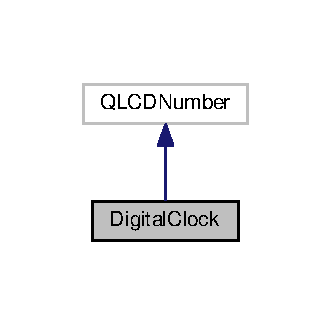
\includegraphics[width=159pt]{classDigitalClock__inherit__graph}
\end{center}
\end{figure}


Collaboration diagram for Digital\+Clock\+:\nopagebreak
\begin{figure}[H]
\begin{center}
\leavevmode
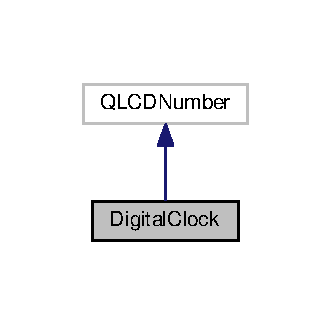
\includegraphics[width=159pt]{classDigitalClock__coll__graph}
\end{center}
\end{figure}
\subsection*{Public Member Functions}
\begin{DoxyCompactItemize}
\item 
\hyperlink{classDigitalClock_af7c214200f518512b56638fb7d568000}{Digital\+Clock} (int \hyperlink{classDigitalClock_adfb81207db5e40a4ccf2b3812632325f}{stop\+After\+Ms}=120000, int \hyperlink{classDigitalClock_a0f09000c25752c09f48e05b96be37ea8}{begin\+Min}=2, int \hyperlink{classDigitalClock_aea23d1b4ccdcd8aa435aaab8d853af57}{begin\+Sec}=0)
\end{DoxyCompactItemize}
\subsection*{Private Slots}
\begin{DoxyCompactItemize}
\item 
void \hyperlink{classDigitalClock_af0c88ea180e73ee60842341790d31b44}{show\+Time} ()
\item 
void \hyperlink{classDigitalClock_af5f394416f4d08f504e88587f60cc489}{stop\+Time} ()
\end{DoxyCompactItemize}
\subsection*{Private Attributes}
\begin{DoxyCompactItemize}
\item 
Q\+Timer $\ast$ \hyperlink{classDigitalClock_a3d92d64a319dca68e29374b3ec4262bf}{container\+Timer}
\item 
Q\+Timer $\ast$ \hyperlink{classDigitalClock_ae0f3267ca73ca79b3a97682c8e0e7d2c}{timer}
\item 
Q\+Time $\ast$ \hyperlink{classDigitalClock_ad093050fd193ddb6080eee02766806b8}{time\+Value}
\item 
int \hyperlink{classDigitalClock_adfb81207db5e40a4ccf2b3812632325f}{stop\+After\+Ms}
\item 
int \hyperlink{classDigitalClock_a0f09000c25752c09f48e05b96be37ea8}{begin\+Min}
\item 
int \hyperlink{classDigitalClock_aea23d1b4ccdcd8aa435aaab8d853af57}{begin\+Sec}
\end{DoxyCompactItemize}


\subsection{Detailed Description}
A class that defines the graphical interface for timer. 

\subsection{Constructor \& Destructor Documentation}
\index{Digital\+Clock@{Digital\+Clock}!Digital\+Clock@{Digital\+Clock}}
\index{Digital\+Clock@{Digital\+Clock}!Digital\+Clock@{Digital\+Clock}}
\subsubsection[{\texorpdfstring{Digital\+Clock(int stop\+After\+Ms=120000, int begin\+Min=2, int begin\+Sec=0)}{DigitalClock(int stopAfterMs=120000, int beginMin=2, int beginSec=0)}}]{\setlength{\rightskip}{0pt plus 5cm}{\bf Digital\+Clock} (
\begin{DoxyParamCaption}
\item[{int}]{stop\+After\+Ms = {\ttfamily 120000}, }
\item[{int}]{begin\+Min = {\ttfamily 2}, }
\item[{int}]{begin\+Sec = {\ttfamily 0}}
\end{DoxyParamCaption}
)}\hypertarget{classDigitalClock_af7c214200f518512b56638fb7d568000}{}\label{classDigitalClock_af7c214200f518512b56638fb7d568000}


\subsection{Member Function Documentation}
\index{Digital\+Clock@{Digital\+Clock}!show\+Time@{show\+Time}}
\index{show\+Time@{show\+Time}!Digital\+Clock@{Digital\+Clock}}
\subsubsection[{\texorpdfstring{show\+Time}{showTime}}]{\setlength{\rightskip}{0pt plus 5cm}void show\+Time (
\begin{DoxyParamCaption}
{}
\end{DoxyParamCaption}
)\hspace{0.3cm}{\ttfamily [private]}, {\ttfamily [slot]}}\hypertarget{classDigitalClock_af0c88ea180e73ee60842341790d31b44}{}\label{classDigitalClock_af0c88ea180e73ee60842341790d31b44}
\index{Digital\+Clock@{Digital\+Clock}!stop\+Time@{stop\+Time}}
\index{stop\+Time@{stop\+Time}!Digital\+Clock@{Digital\+Clock}}
\subsubsection[{\texorpdfstring{stop\+Time}{stopTime}}]{\setlength{\rightskip}{0pt plus 5cm}void stop\+Time (
\begin{DoxyParamCaption}
{}
\end{DoxyParamCaption}
)\hspace{0.3cm}{\ttfamily [private]}, {\ttfamily [slot]}}\hypertarget{classDigitalClock_af5f394416f4d08f504e88587f60cc489}{}\label{classDigitalClock_af5f394416f4d08f504e88587f60cc489}


\subsection{Member Data Documentation}
\index{Digital\+Clock@{Digital\+Clock}!begin\+Min@{begin\+Min}}
\index{begin\+Min@{begin\+Min}!Digital\+Clock@{Digital\+Clock}}
\subsubsection[{\texorpdfstring{begin\+Min}{beginMin}}]{\setlength{\rightskip}{0pt plus 5cm}int begin\+Min\hspace{0.3cm}{\ttfamily [private]}}\hypertarget{classDigitalClock_a0f09000c25752c09f48e05b96be37ea8}{}\label{classDigitalClock_a0f09000c25752c09f48e05b96be37ea8}
\index{Digital\+Clock@{Digital\+Clock}!begin\+Sec@{begin\+Sec}}
\index{begin\+Sec@{begin\+Sec}!Digital\+Clock@{Digital\+Clock}}
\subsubsection[{\texorpdfstring{begin\+Sec}{beginSec}}]{\setlength{\rightskip}{0pt plus 5cm}int begin\+Sec\hspace{0.3cm}{\ttfamily [private]}}\hypertarget{classDigitalClock_aea23d1b4ccdcd8aa435aaab8d853af57}{}\label{classDigitalClock_aea23d1b4ccdcd8aa435aaab8d853af57}
\index{Digital\+Clock@{Digital\+Clock}!container\+Timer@{container\+Timer}}
\index{container\+Timer@{container\+Timer}!Digital\+Clock@{Digital\+Clock}}
\subsubsection[{\texorpdfstring{container\+Timer}{containerTimer}}]{\setlength{\rightskip}{0pt plus 5cm}Q\+Timer$\ast$ container\+Timer\hspace{0.3cm}{\ttfamily [private]}}\hypertarget{classDigitalClock_a3d92d64a319dca68e29374b3ec4262bf}{}\label{classDigitalClock_a3d92d64a319dca68e29374b3ec4262bf}
\index{Digital\+Clock@{Digital\+Clock}!stop\+After\+Ms@{stop\+After\+Ms}}
\index{stop\+After\+Ms@{stop\+After\+Ms}!Digital\+Clock@{Digital\+Clock}}
\subsubsection[{\texorpdfstring{stop\+After\+Ms}{stopAfterMs}}]{\setlength{\rightskip}{0pt plus 5cm}int stop\+After\+Ms\hspace{0.3cm}{\ttfamily [private]}}\hypertarget{classDigitalClock_adfb81207db5e40a4ccf2b3812632325f}{}\label{classDigitalClock_adfb81207db5e40a4ccf2b3812632325f}
\index{Digital\+Clock@{Digital\+Clock}!timer@{timer}}
\index{timer@{timer}!Digital\+Clock@{Digital\+Clock}}
\subsubsection[{\texorpdfstring{timer}{timer}}]{\setlength{\rightskip}{0pt plus 5cm}Q\+Timer$\ast$ timer\hspace{0.3cm}{\ttfamily [private]}}\hypertarget{classDigitalClock_ae0f3267ca73ca79b3a97682c8e0e7d2c}{}\label{classDigitalClock_ae0f3267ca73ca79b3a97682c8e0e7d2c}
\index{Digital\+Clock@{Digital\+Clock}!time\+Value@{time\+Value}}
\index{time\+Value@{time\+Value}!Digital\+Clock@{Digital\+Clock}}
\subsubsection[{\texorpdfstring{time\+Value}{timeValue}}]{\setlength{\rightskip}{0pt plus 5cm}Q\+Time$\ast$ time\+Value\hspace{0.3cm}{\ttfamily [private]}}\hypertarget{classDigitalClock_ad093050fd193ddb6080eee02766806b8}{}\label{classDigitalClock_ad093050fd193ddb6080eee02766806b8}


The documentation for this class was generated from the following files\+:\begin{DoxyCompactItemize}
\item 
gui/\hyperlink{digitalclock_8h}{digitalclock.\+h}\item 
gui/\hyperlink{digitalclock_8cpp}{digitalclock.\+cpp}\end{DoxyCompactItemize}

\hypertarget{classMODEL_1_1Game}{}\section{Game Class Reference}
\label{classMODEL_1_1Game}\index{Game@{Game}}


A class representing game session that access both \hyperlink{classMODEL_1_1Player}{Player} and \hyperlink{classMODEL_1_1Communicator}{Communicator}.  




{\ttfamily \#include $<$game.\+h$>$}



Inheritance diagram for Game\+:\nopagebreak
\begin{figure}[H]
\begin{center}
\leavevmode
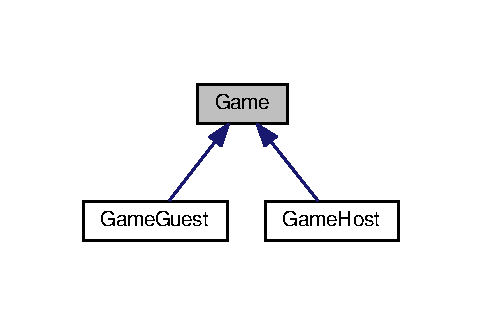
\includegraphics[width=232pt]{classMODEL_1_1Game__inherit__graph}
\end{center}
\end{figure}


Collaboration diagram for Game\+:\nopagebreak
\begin{figure}[H]
\begin{center}
\leavevmode
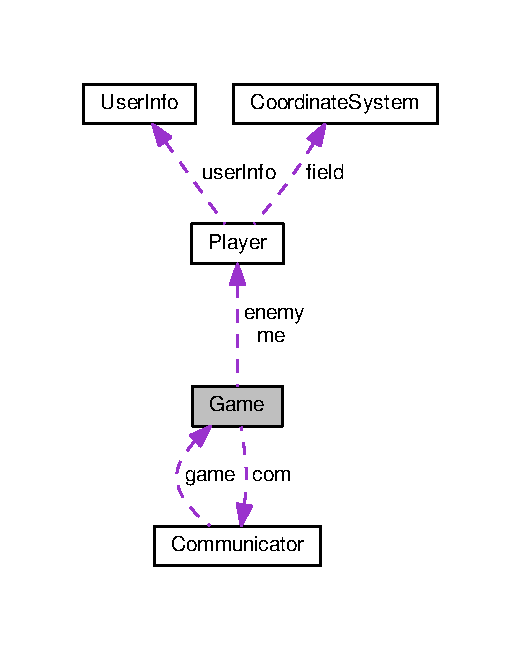
\includegraphics[width=250pt]{classMODEL_1_1Game__coll__graph}
\end{center}
\end{figure}
\subsection*{Public Member Functions}
\begin{DoxyCompactItemize}
\item 
virtual \hyperlink{classMODEL_1_1Game_ac168f724bc6694d4f9d4c87f8c0189ba}{$\sim$\+Game} ()
\item 
void \hyperlink{classMODEL_1_1Game_a3a9f3966eb6f57eac31e4d6244c07c58}{place\+Ship} (\hyperlink{classMODEL_1_1Point}{Point} p1, \hyperlink{classMODEL_1_1Point}{Point} p2)
\end{DoxyCompactItemize}
\subsection*{Protected Member Functions}
\begin{DoxyCompactItemize}
\item 
\hyperlink{classMODEL_1_1Game_a12daf58e448825c36267d00317e106ab}{Game} (std\+::vector$<$ std\+::reference\+\_\+wrapper$<$ \hyperlink{classBattleshipObserver}{Battleship\+Observer} $>$$>$ \&\hyperlink{classMODEL_1_1Game_afada2cb52f9872db4f3ab6e72d07cd05}{observer\+List}, \hyperlink{classUserInfo}{User\+Info} \hyperlink{classUserInfo}{User\+Info})
\item 
\hyperlink{classMODEL_1_1Game_a088a17112f1a818f00c0da4bd4d18c1c}{Game} (const std\+::string \&address, int port, std\+::vector$<$ std\+::reference\+\_\+wrapper$<$ \hyperlink{classBattleshipObserver}{Battleship\+Observer} $>$$>$ \&\hyperlink{classMODEL_1_1Game_afada2cb52f9872db4f3ab6e72d07cd05}{observer\+List}, \hyperlink{classUserInfo}{User\+Info} \hyperlink{classUserInfo}{User\+Info})
\item 
\hyperlink{classMODEL_1_1Game_aade93aad98ae9bc9931236d08f48fcf3}{Game} (\hyperlink{classMODEL_1_1Game}{Game} const \&)=delete
\item 
\hyperlink{classMODEL_1_1Game}{Game} \& \hyperlink{classMODEL_1_1Game_a09ee8455dc72eb38e41bb59d70158bb1}{operator=} (\hyperlink{classMODEL_1_1Game}{Game} const \&other)=delete
\item 
\hyperlink{classMODEL_1_1Game_a71b42b0e2d234b1240823a01cfd13e66}{Game} (\hyperlink{classMODEL_1_1Game}{Game} \&\&other)=delete
\item 
\hyperlink{classMODEL_1_1Game}{Game} \& \hyperlink{classMODEL_1_1Game_ad1c94ba579ec1ea46b7a534b3443199d}{operator=} (\hyperlink{classMODEL_1_1Game}{Game} \&\&other)=delete
\item 
void \hyperlink{classMODEL_1_1Game_a7e0a9af181a76ce2bf8ce1e11f5e03ab}{socket\+Connected} ()
\end{DoxyCompactItemize}
\subsection*{Protected Attributes}
\begin{DoxyCompactItemize}
\item 
std\+::vector$<$ std\+::reference\+\_\+wrapper$<$ \hyperlink{classBattleshipObserver}{Battleship\+Observer} $>$ $>$ \& \hyperlink{classMODEL_1_1Game_afada2cb52f9872db4f3ab6e72d07cd05}{observer\+List}
\item 
\hyperlink{classMODEL_1_1Player}{M\+O\+D\+E\+L\+::\+Player} \hyperlink{classMODEL_1_1Game_ab8c6b1da146382b3d0d098e55cf4b54f}{me}
\item 
\hyperlink{classMODEL_1_1Player}{M\+O\+D\+E\+L\+::\+Player} \hyperlink{classMODEL_1_1Game_a9d4d84ca610764d9de0ca5cca663dc17}{enemy}
\end{DoxyCompactItemize}
\subsection*{Private Attributes}
\begin{DoxyCompactItemize}
\item 
\hyperlink{classMODEL_1_1Communicator}{Communicator} \hyperlink{classMODEL_1_1Game_ad4cdd6f3873de65537dda44338624c21}{com}
\end{DoxyCompactItemize}


\subsection{Detailed Description}
A class representing game session that access both \hyperlink{classMODEL_1_1Player}{Player} and \hyperlink{classMODEL_1_1Communicator}{Communicator}. 

\subsection{Constructor \& Destructor Documentation}
\index{M\+O\+D\+E\+L\+::\+Game@{M\+O\+D\+E\+L\+::\+Game}!````~Game@{$\sim$\+Game}}
\index{````~Game@{$\sim$\+Game}!M\+O\+D\+E\+L\+::\+Game@{M\+O\+D\+E\+L\+::\+Game}}
\subsubsection[{\texorpdfstring{$\sim$\+Game()}{~Game()}}]{\setlength{\rightskip}{0pt plus 5cm}$\sim${\bf Game} (
\begin{DoxyParamCaption}
{}
\end{DoxyParamCaption}
)\hspace{0.3cm}{\ttfamily [virtual]}}\hypertarget{classMODEL_1_1Game_ac168f724bc6694d4f9d4c87f8c0189ba}{}\label{classMODEL_1_1Game_ac168f724bc6694d4f9d4c87f8c0189ba}
\index{M\+O\+D\+E\+L\+::\+Game@{M\+O\+D\+E\+L\+::\+Game}!Game@{Game}}
\index{Game@{Game}!M\+O\+D\+E\+L\+::\+Game@{M\+O\+D\+E\+L\+::\+Game}}
\subsubsection[{\texorpdfstring{Game(std\+::vector$<$ std\+::reference\+\_\+wrapper$<$ Battleship\+Observer $>$$>$ \&observer\+List, User\+Info User\+Info)}{Game(std::vector< std::reference_wrapper< BattleshipObserver >> &observerList, UserInfo UserInfo)}}]{\setlength{\rightskip}{0pt plus 5cm}{\bf Game} (
\begin{DoxyParamCaption}
\item[{std\+::vector$<$ std\+::reference\+\_\+wrapper$<$ {\bf Battleship\+Observer} $>$$>$ \&}]{observer\+List, }
\item[{{\bf User\+Info}}]{User\+Info}
\end{DoxyParamCaption}
)\hspace{0.3cm}{\ttfamily [explicit]}, {\ttfamily [protected]}}\hypertarget{classMODEL_1_1Game_a12daf58e448825c36267d00317e106ab}{}\label{classMODEL_1_1Game_a12daf58e448825c36267d00317e106ab}
constructor used in \hyperlink{classMODEL_1_1GameHost}{Game\+Host} class \index{M\+O\+D\+E\+L\+::\+Game@{M\+O\+D\+E\+L\+::\+Game}!Game@{Game}}
\index{Game@{Game}!M\+O\+D\+E\+L\+::\+Game@{M\+O\+D\+E\+L\+::\+Game}}
\subsubsection[{\texorpdfstring{Game(const std\+::string \&address, int port, std\+::vector$<$ std\+::reference\+\_\+wrapper$<$ Battleship\+Observer $>$$>$ \&observer\+List, User\+Info User\+Info)}{Game(const std::string &address, int port, std::vector< std::reference_wrapper< BattleshipObserver >> &observerList, UserInfo UserInfo)}}]{\setlength{\rightskip}{0pt plus 5cm}{\bf Game} (
\begin{DoxyParamCaption}
\item[{const std\+::string \&}]{address, }
\item[{int}]{port, }
\item[{std\+::vector$<$ std\+::reference\+\_\+wrapper$<$ {\bf Battleship\+Observer} $>$$>$ \&}]{observer\+List, }
\item[{{\bf User\+Info}}]{User\+Info}
\end{DoxyParamCaption}
)\hspace{0.3cm}{\ttfamily [explicit]}, {\ttfamily [protected]}}\hypertarget{classMODEL_1_1Game_a088a17112f1a818f00c0da4bd4d18c1c}{}\label{classMODEL_1_1Game_a088a17112f1a818f00c0da4bd4d18c1c}
constructor used in \hyperlink{classMODEL_1_1GameGuest}{Game\+Guest} class \index{M\+O\+D\+E\+L\+::\+Game@{M\+O\+D\+E\+L\+::\+Game}!Game@{Game}}
\index{Game@{Game}!M\+O\+D\+E\+L\+::\+Game@{M\+O\+D\+E\+L\+::\+Game}}
\subsubsection[{\texorpdfstring{Game(\+Game const \&)=delete}{Game(Game const &)=delete}}]{\setlength{\rightskip}{0pt plus 5cm}{\bf Game} (
\begin{DoxyParamCaption}
\item[{{\bf Game} const \&}]{}
\end{DoxyParamCaption}
)\hspace{0.3cm}{\ttfamily [protected]}, {\ttfamily [delete]}}\hypertarget{classMODEL_1_1Game_aade93aad98ae9bc9931236d08f48fcf3}{}\label{classMODEL_1_1Game_aade93aad98ae9bc9931236d08f48fcf3}
\index{M\+O\+D\+E\+L\+::\+Game@{M\+O\+D\+E\+L\+::\+Game}!Game@{Game}}
\index{Game@{Game}!M\+O\+D\+E\+L\+::\+Game@{M\+O\+D\+E\+L\+::\+Game}}
\subsubsection[{\texorpdfstring{Game(\+Game \&\&other)=delete}{Game(Game &&other)=delete}}]{\setlength{\rightskip}{0pt plus 5cm}{\bf Game} (
\begin{DoxyParamCaption}
\item[{{\bf Game} \&\&}]{other}
\end{DoxyParamCaption}
)\hspace{0.3cm}{\ttfamily [protected]}, {\ttfamily [delete]}}\hypertarget{classMODEL_1_1Game_a71b42b0e2d234b1240823a01cfd13e66}{}\label{classMODEL_1_1Game_a71b42b0e2d234b1240823a01cfd13e66}


\subsection{Member Function Documentation}
\index{M\+O\+D\+E\+L\+::\+Game@{M\+O\+D\+E\+L\+::\+Game}!operator=@{operator=}}
\index{operator=@{operator=}!M\+O\+D\+E\+L\+::\+Game@{M\+O\+D\+E\+L\+::\+Game}}
\subsubsection[{\texorpdfstring{operator=(\+Game const \&other)=delete}{operator=(Game const &other)=delete}}]{\setlength{\rightskip}{0pt plus 5cm}{\bf Game}\& operator= (
\begin{DoxyParamCaption}
\item[{{\bf Game} const \&}]{other}
\end{DoxyParamCaption}
)\hspace{0.3cm}{\ttfamily [protected]}, {\ttfamily [delete]}}\hypertarget{classMODEL_1_1Game_a09ee8455dc72eb38e41bb59d70158bb1}{}\label{classMODEL_1_1Game_a09ee8455dc72eb38e41bb59d70158bb1}
\index{M\+O\+D\+E\+L\+::\+Game@{M\+O\+D\+E\+L\+::\+Game}!operator=@{operator=}}
\index{operator=@{operator=}!M\+O\+D\+E\+L\+::\+Game@{M\+O\+D\+E\+L\+::\+Game}}
\subsubsection[{\texorpdfstring{operator=(\+Game \&\&other)=delete}{operator=(Game &&other)=delete}}]{\setlength{\rightskip}{0pt plus 5cm}{\bf Game}\& operator= (
\begin{DoxyParamCaption}
\item[{{\bf Game} \&\&}]{other}
\end{DoxyParamCaption}
)\hspace{0.3cm}{\ttfamily [protected]}, {\ttfamily [delete]}}\hypertarget{classMODEL_1_1Game_ad1c94ba579ec1ea46b7a534b3443199d}{}\label{classMODEL_1_1Game_ad1c94ba579ec1ea46b7a534b3443199d}
\index{M\+O\+D\+E\+L\+::\+Game@{M\+O\+D\+E\+L\+::\+Game}!place\+Ship@{place\+Ship}}
\index{place\+Ship@{place\+Ship}!M\+O\+D\+E\+L\+::\+Game@{M\+O\+D\+E\+L\+::\+Game}}
\subsubsection[{\texorpdfstring{place\+Ship(\+Point p1, Point p2)}{placeShip(Point p1, Point p2)}}]{\setlength{\rightskip}{0pt plus 5cm}void place\+Ship (
\begin{DoxyParamCaption}
\item[{{\bf M\+O\+D\+E\+L\+::\+Point}}]{p1, }
\item[{{\bf M\+O\+D\+E\+L\+::\+Point}}]{p2}
\end{DoxyParamCaption}
)}\hypertarget{classMODEL_1_1Game_a3a9f3966eb6f57eac31e4d6244c07c58}{}\label{classMODEL_1_1Game_a3a9f3966eb6f57eac31e4d6244c07c58}
\begin{DoxySeeAlso}{See also}
\hyperlink{classModelInterface_aa708cd5411011ade34c2796b3f102612}{Model\+Interface\+::place\+Ship(\+M\+O\+D\+E\+L\+::\+Point, M\+O\+D\+E\+L\+::\+Point)} 
\end{DoxySeeAlso}
\index{M\+O\+D\+E\+L\+::\+Game@{M\+O\+D\+E\+L\+::\+Game}!socket\+Connected@{socket\+Connected}}
\index{socket\+Connected@{socket\+Connected}!M\+O\+D\+E\+L\+::\+Game@{M\+O\+D\+E\+L\+::\+Game}}
\subsubsection[{\texorpdfstring{socket\+Connected()}{socketConnected()}}]{\setlength{\rightskip}{0pt plus 5cm}void socket\+Connected (
\begin{DoxyParamCaption}
{}
\end{DoxyParamCaption}
)\hspace{0.3cm}{\ttfamily [protected]}}\hypertarget{classMODEL_1_1Game_a7e0a9af181a76ce2bf8ce1e11f5e03ab}{}\label{classMODEL_1_1Game_a7e0a9af181a76ce2bf8ce1e11f5e03ab}


\subsection{Member Data Documentation}
\index{M\+O\+D\+E\+L\+::\+Game@{M\+O\+D\+E\+L\+::\+Game}!com@{com}}
\index{com@{com}!M\+O\+D\+E\+L\+::\+Game@{M\+O\+D\+E\+L\+::\+Game}}
\subsubsection[{\texorpdfstring{com}{com}}]{\setlength{\rightskip}{0pt plus 5cm}{\bf Communicator} com\hspace{0.3cm}{\ttfamily [private]}}\hypertarget{classMODEL_1_1Game_ad4cdd6f3873de65537dda44338624c21}{}\label{classMODEL_1_1Game_ad4cdd6f3873de65537dda44338624c21}
\index{M\+O\+D\+E\+L\+::\+Game@{M\+O\+D\+E\+L\+::\+Game}!enemy@{enemy}}
\index{enemy@{enemy}!M\+O\+D\+E\+L\+::\+Game@{M\+O\+D\+E\+L\+::\+Game}}
\subsubsection[{\texorpdfstring{enemy}{enemy}}]{\setlength{\rightskip}{0pt plus 5cm}{\bf M\+O\+D\+E\+L\+::\+Player} enemy\hspace{0.3cm}{\ttfamily [protected]}}\hypertarget{classMODEL_1_1Game_a9d4d84ca610764d9de0ca5cca663dc17}{}\label{classMODEL_1_1Game_a9d4d84ca610764d9de0ca5cca663dc17}
\index{M\+O\+D\+E\+L\+::\+Game@{M\+O\+D\+E\+L\+::\+Game}!me@{me}}
\index{me@{me}!M\+O\+D\+E\+L\+::\+Game@{M\+O\+D\+E\+L\+::\+Game}}
\subsubsection[{\texorpdfstring{me}{me}}]{\setlength{\rightskip}{0pt plus 5cm}{\bf M\+O\+D\+E\+L\+::\+Player} me\hspace{0.3cm}{\ttfamily [protected]}}\hypertarget{classMODEL_1_1Game_ab8c6b1da146382b3d0d098e55cf4b54f}{}\label{classMODEL_1_1Game_ab8c6b1da146382b3d0d098e55cf4b54f}
\index{M\+O\+D\+E\+L\+::\+Game@{M\+O\+D\+E\+L\+::\+Game}!observer\+List@{observer\+List}}
\index{observer\+List@{observer\+List}!M\+O\+D\+E\+L\+::\+Game@{M\+O\+D\+E\+L\+::\+Game}}
\subsubsection[{\texorpdfstring{observer\+List}{observerList}}]{\setlength{\rightskip}{0pt plus 5cm}std\+::vector$<$std\+::reference\+\_\+wrapper$<${\bf Battleship\+Observer}$>$ $>$\& observer\+List\hspace{0.3cm}{\ttfamily [protected]}}\hypertarget{classMODEL_1_1Game_afada2cb52f9872db4f3ab6e72d07cd05}{}\label{classMODEL_1_1Game_afada2cb52f9872db4f3ab6e72d07cd05}


The documentation for this class was generated from the following files\+:\begin{DoxyCompactItemize}
\item 
model/\hyperlink{game_8h}{game.\+h}\item 
model/\hyperlink{game_8cpp}{game.\+cpp}\end{DoxyCompactItemize}

\hypertarget{classGUI_1_1GameCoordinateSystem}{}\section{Game\+Coordinate\+System Class Reference}
\label{classGUI_1_1GameCoordinateSystem}\index{Game\+Coordinate\+System@{Game\+Coordinate\+System}}


A simple class that inherits from \hyperlink{classGUI_1_1CoordinateSystem}{Coordinate\+System} and implements mouse events for starting attack.  




{\ttfamily \#include $<$gamecoordinatesystem.\+h$>$}



Inheritance diagram for Game\+Coordinate\+System\+:\nopagebreak
\begin{figure}[H]
\begin{center}
\leavevmode
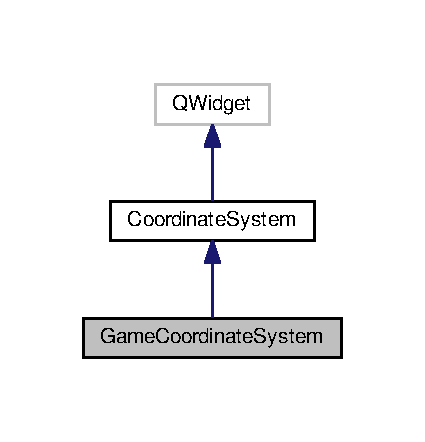
\includegraphics[width=204pt]{classGUI_1_1GameCoordinateSystem__inherit__graph}
\end{center}
\end{figure}


Collaboration diagram for Game\+Coordinate\+System\+:\nopagebreak
\begin{figure}[H]
\begin{center}
\leavevmode
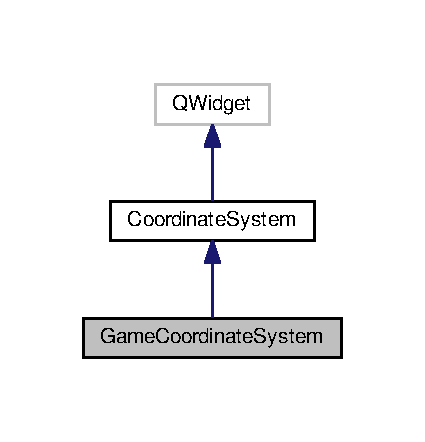
\includegraphics[width=204pt]{classGUI_1_1GameCoordinateSystem__coll__graph}
\end{center}
\end{figure}
\subsection*{Public Member Functions}
\begin{DoxyCompactItemize}
\item 
\hyperlink{classGUI_1_1GameCoordinateSystem_ad90026545ab4130f336058ad6e56a7ae}{$\sim$\+Game\+Coordinate\+System} ()
\item 
void \hyperlink{classGUI_1_1GameCoordinateSystem_a9458976a8507b7cf973c20418fb667a4}{paint\+Shots} ()
\item 
void \hyperlink{classGUI_1_1GameCoordinateSystem_afcf62685a11ce5529786cc14ddecc7f2}{clear\+Field} ()
\begin{DoxyCompactList}\small\item\em Eine Funktion, die pure virtual ist, wird fuer eine abstrakte Klasse benoetigt. \end{DoxyCompactList}\item 
void \hyperlink{classGUI_1_1GameCoordinateSystem_ad2272e344e46519f026cd02f419884f1}{mouse\+Press\+Event} (Q\+Mouse\+Event $\ast$event)
\item 
void \hyperlink{classGUI_1_1GameCoordinateSystem_a35226f6549add1ff837c65888fcd00fc}{mouse\+Release\+Event} (Q\+Mouse\+Event $\ast$event)
\item 
void \hyperlink{classGUI_1_1GameCoordinateSystem_ae820c6a86f0a1908bf451f86db043489}{mouse\+Move\+Event} (Q\+Mouse\+Event $\ast$event)
\item 
void \hyperlink{classGUI_1_1GameCoordinateSystem_accfb24f32254fb98c049727597a53956}{paint\+Event} (Q\+Paint\+Event $\ast$event)
\end{DoxyCompactItemize}
\subsection*{Additional Inherited Members}


\subsection{Detailed Description}
A simple class that inherits from \hyperlink{classGUI_1_1CoordinateSystem}{Coordinate\+System} and implements mouse events for starting attack. 

\subsection{Constructor \& Destructor Documentation}
\index{G\+U\+I\+::\+Game\+Coordinate\+System@{G\+U\+I\+::\+Game\+Coordinate\+System}!````~Game\+Coordinate\+System@{$\sim$\+Game\+Coordinate\+System}}
\index{````~Game\+Coordinate\+System@{$\sim$\+Game\+Coordinate\+System}!G\+U\+I\+::\+Game\+Coordinate\+System@{G\+U\+I\+::\+Game\+Coordinate\+System}}
\subsubsection[{\texorpdfstring{$\sim$\+Game\+Coordinate\+System()}{~GameCoordinateSystem()}}]{\setlength{\rightskip}{0pt plus 5cm}$\sim${\bf Game\+Coordinate\+System} (
\begin{DoxyParamCaption}
{}
\end{DoxyParamCaption}
)}\hypertarget{classGUI_1_1GameCoordinateSystem_ad90026545ab4130f336058ad6e56a7ae}{}\label{classGUI_1_1GameCoordinateSystem_ad90026545ab4130f336058ad6e56a7ae}


\subsection{Member Function Documentation}
\index{G\+U\+I\+::\+Game\+Coordinate\+System@{G\+U\+I\+::\+Game\+Coordinate\+System}!clear\+Field@{clear\+Field}}
\index{clear\+Field@{clear\+Field}!G\+U\+I\+::\+Game\+Coordinate\+System@{G\+U\+I\+::\+Game\+Coordinate\+System}}
\subsubsection[{\texorpdfstring{clear\+Field()}{clearField()}}]{\setlength{\rightskip}{0pt plus 5cm}void clear\+Field (
\begin{DoxyParamCaption}
{}
\end{DoxyParamCaption}
)\hspace{0.3cm}{\ttfamily [virtual]}}\hypertarget{classGUI_1_1GameCoordinateSystem_afcf62685a11ce5529786cc14ddecc7f2}{}\label{classGUI_1_1GameCoordinateSystem_afcf62685a11ce5529786cc14ddecc7f2}


Eine Funktion, die pure virtual ist, wird fuer eine abstrakte Klasse benoetigt. 



Implements \hyperlink{classGUI_1_1CoordinateSystem_a3d41bd83deb883b8d0c8d192bd0b1ddd}{Coordinate\+System}.

\index{G\+U\+I\+::\+Game\+Coordinate\+System@{G\+U\+I\+::\+Game\+Coordinate\+System}!mouse\+Move\+Event@{mouse\+Move\+Event}}
\index{mouse\+Move\+Event@{mouse\+Move\+Event}!G\+U\+I\+::\+Game\+Coordinate\+System@{G\+U\+I\+::\+Game\+Coordinate\+System}}
\subsubsection[{\texorpdfstring{mouse\+Move\+Event(\+Q\+Mouse\+Event $\ast$event)}{mouseMoveEvent(QMouseEvent *event)}}]{\setlength{\rightskip}{0pt plus 5cm}void mouse\+Move\+Event (
\begin{DoxyParamCaption}
\item[{Q\+Mouse\+Event $\ast$}]{event}
\end{DoxyParamCaption}
)}\hypertarget{classGUI_1_1GameCoordinateSystem_ae820c6a86f0a1908bf451f86db043489}{}\label{classGUI_1_1GameCoordinateSystem_ae820c6a86f0a1908bf451f86db043489}
\index{G\+U\+I\+::\+Game\+Coordinate\+System@{G\+U\+I\+::\+Game\+Coordinate\+System}!mouse\+Press\+Event@{mouse\+Press\+Event}}
\index{mouse\+Press\+Event@{mouse\+Press\+Event}!G\+U\+I\+::\+Game\+Coordinate\+System@{G\+U\+I\+::\+Game\+Coordinate\+System}}
\subsubsection[{\texorpdfstring{mouse\+Press\+Event(\+Q\+Mouse\+Event $\ast$event)}{mousePressEvent(QMouseEvent *event)}}]{\setlength{\rightskip}{0pt plus 5cm}void mouse\+Press\+Event (
\begin{DoxyParamCaption}
\item[{Q\+Mouse\+Event $\ast$}]{event}
\end{DoxyParamCaption}
)}\hypertarget{classGUI_1_1GameCoordinateSystem_ad2272e344e46519f026cd02f419884f1}{}\label{classGUI_1_1GameCoordinateSystem_ad2272e344e46519f026cd02f419884f1}
\index{G\+U\+I\+::\+Game\+Coordinate\+System@{G\+U\+I\+::\+Game\+Coordinate\+System}!mouse\+Release\+Event@{mouse\+Release\+Event}}
\index{mouse\+Release\+Event@{mouse\+Release\+Event}!G\+U\+I\+::\+Game\+Coordinate\+System@{G\+U\+I\+::\+Game\+Coordinate\+System}}
\subsubsection[{\texorpdfstring{mouse\+Release\+Event(\+Q\+Mouse\+Event $\ast$event)}{mouseReleaseEvent(QMouseEvent *event)}}]{\setlength{\rightskip}{0pt plus 5cm}void mouse\+Release\+Event (
\begin{DoxyParamCaption}
\item[{Q\+Mouse\+Event $\ast$}]{event}
\end{DoxyParamCaption}
)}\hypertarget{classGUI_1_1GameCoordinateSystem_a35226f6549add1ff837c65888fcd00fc}{}\label{classGUI_1_1GameCoordinateSystem_a35226f6549add1ff837c65888fcd00fc}
\index{G\+U\+I\+::\+Game\+Coordinate\+System@{G\+U\+I\+::\+Game\+Coordinate\+System}!paint\+Event@{paint\+Event}}
\index{paint\+Event@{paint\+Event}!G\+U\+I\+::\+Game\+Coordinate\+System@{G\+U\+I\+::\+Game\+Coordinate\+System}}
\subsubsection[{\texorpdfstring{paint\+Event(\+Q\+Paint\+Event $\ast$event)}{paintEvent(QPaintEvent *event)}}]{\setlength{\rightskip}{0pt plus 5cm}void paint\+Event (
\begin{DoxyParamCaption}
\item[{Q\+Paint\+Event $\ast$}]{event}
\end{DoxyParamCaption}
)}\hypertarget{classGUI_1_1GameCoordinateSystem_accfb24f32254fb98c049727597a53956}{}\label{classGUI_1_1GameCoordinateSystem_accfb24f32254fb98c049727597a53956}
\index{G\+U\+I\+::\+Game\+Coordinate\+System@{G\+U\+I\+::\+Game\+Coordinate\+System}!paint\+Shots@{paint\+Shots}}
\index{paint\+Shots@{paint\+Shots}!G\+U\+I\+::\+Game\+Coordinate\+System@{G\+U\+I\+::\+Game\+Coordinate\+System}}
\subsubsection[{\texorpdfstring{paint\+Shots()}{paintShots()}}]{\setlength{\rightskip}{0pt plus 5cm}void paint\+Shots (
\begin{DoxyParamCaption}
{}
\end{DoxyParamCaption}
)}\hypertarget{classGUI_1_1GameCoordinateSystem_a9458976a8507b7cf973c20418fb667a4}{}\label{classGUI_1_1GameCoordinateSystem_a9458976a8507b7cf973c20418fb667a4}


The documentation for this class was generated from the following files\+:\begin{DoxyCompactItemize}
\item 
gui/\hyperlink{gamecoordinatesystem_8h}{gamecoordinatesystem.\+h}\item 
gui/\hyperlink{gamecoordinatesystem_8cpp}{gamecoordinatesystem.\+cpp}\end{DoxyCompactItemize}

\hypertarget{classGameForm}{}\section{Game\+Form Class Reference}
\label{classGameForm}\index{Game\+Form@{Game\+Form}}


A simple class that defines graphical interface of the form in which players are able to attack, recieve attack, etc.  




{\ttfamily \#include $<$gameform.\+h$>$}



Inheritance diagram for Game\+Form\+:\nopagebreak
\begin{figure}[H]
\begin{center}
\leavevmode
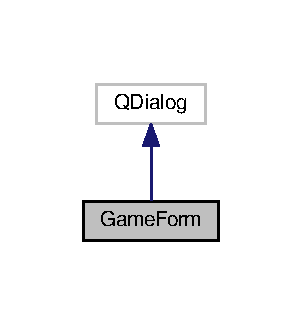
\includegraphics[width=145pt]{classGameForm__inherit__graph}
\end{center}
\end{figure}


Collaboration diagram for Game\+Form\+:\nopagebreak
\begin{figure}[H]
\begin{center}
\leavevmode
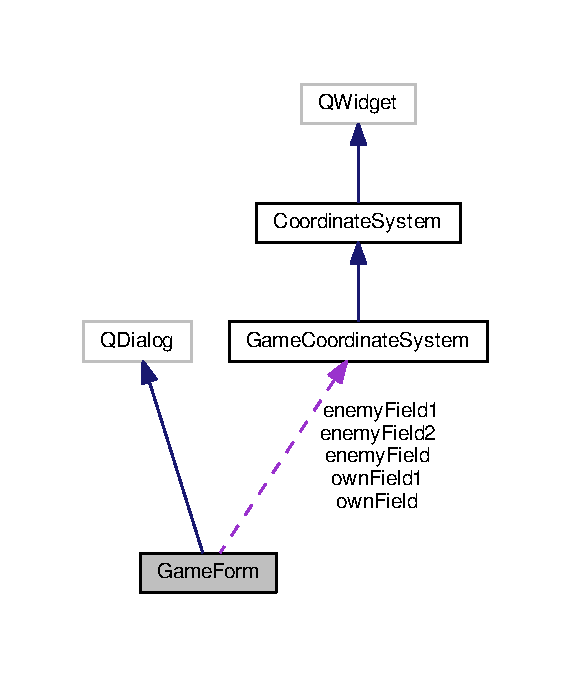
\includegraphics[width=274pt]{classGameForm__coll__graph}
\end{center}
\end{figure}
\subsection*{Public Member Functions}
\begin{DoxyCompactItemize}
\item 
\hyperlink{classGameForm_ae853c67cf61b3a8128ded1b1c18171cb}{Game\+Form} ()
\item 
\hyperlink{classGameForm_a8020ae990541b81e274d003ed1eeeb59}{$\sim$\+Game\+Form} ()
\end{DoxyCompactItemize}
\subsection*{Public Attributes}
\begin{DoxyCompactItemize}
\item 
Q\+String \hyperlink{classGameForm_a6b42c6ec1657cd85c98c46fcfd126046}{status\+Box\+Text} = \char`\"{}\char`\"{}
\end{DoxyCompactItemize}
\subsection*{Private Slots}
\begin{DoxyCompactItemize}
\item 
void \hyperlink{classGameForm_a8b722117b1f1f02aeb60af137ee2d446}{open\+Version} ()
\item 
void \hyperlink{classGameForm_a57fd57ebca600cae3a27f5c768cf0e2d}{reset\+Own\+Field} ()
\item 
void \hyperlink{classGameForm_acc5a7e6e3595b7a835ed0ad3aeb4df73}{check\+Straight} ()
\end{DoxyCompactItemize}
\subsection*{Private Member Functions}
\begin{DoxyCompactItemize}
\item 
void \hyperlink{classGameForm_a5c788b6fcb676c3e1cef7e01eed9a420}{create\+Menus} ()
\item 
void \hyperlink{classGameForm_aacac9e13e6b6a0e20730e8fc831fbf75}{create\+Coordinate\+System\+Group\+Box\+Own} ()
\item 
void \hyperlink{classGameForm_a26921e3aabc5bc459af0414c3ab4de06}{create\+Coordinate\+System\+Group\+Box\+Enemy} ()
\item 
void \hyperlink{classGameForm_ac4d7e3039b39795dcc72a68cc7324e1e}{create\+Information\+Group\+Box} ()
\end{DoxyCompactItemize}
\subsection*{Private Attributes}
\begin{DoxyCompactItemize}
\item 
\hyperlink{classGUI_1_1GameCoordinateSystem}{G\+U\+I\+::\+Game\+Coordinate\+System} $\ast$ \hyperlink{classGameForm_a3f769801cb22e13a5a878fcdc0518d05}{own\+Field}
\item 
\hyperlink{classGUI_1_1GameCoordinateSystem}{G\+U\+I\+::\+Game\+Coordinate\+System} $\ast$ \hyperlink{classGameForm_a2961c0b23c7112cbc62af053e164b322}{enemy\+Field}
\item 
Q\+Group\+Box $\ast$ \hyperlink{classGameForm_ad18a9191e99822758eb03d5ed5e86e31}{coordinate\+System\+Group\+Box\+Own}
\item 
Q\+Group\+Box $\ast$ \hyperlink{classGameForm_a8bdbfc571a3841ecd4e94c8c79deb480}{coordinate\+System\+Group\+Box\+Enemy}
\item 
Q\+Menu\+Bar $\ast$ \hyperlink{classGameForm_af1e1fab084abbaa2eb09807c6f403a9b}{menu\+Bar}
\item 
Q\+Menu $\ast$ \hyperlink{classGameForm_adb1ab65d1aecac73e58f48557c143b2e}{file\+Menu}
\item 
Q\+Menu $\ast$ \hyperlink{classGameForm_ac589920cc2b87288e454430daa93a976}{help\+Menu}
\item 
Q\+Action $\ast$ \hyperlink{classGameForm_adb8d61a6d4522657760029f301a75497}{reset\+Action}
\item 
Q\+Action $\ast$ \hyperlink{classGameForm_a95088aac220cb7eb4159ab75d86cb81d}{exit\+Action}
\item 
Q\+Action $\ast$ \hyperlink{classGameForm_a4f38a2d30e7f01b923b0d9e3f9f2e048}{version\+Action}
\item 
Q\+Group\+Box $\ast$ \hyperlink{classGameForm_a37c93b300cdcf03835fe5f67b43eb08d}{grid\+Group\+Box\+Enemy}
\item 
Q\+Group\+Box $\ast$ \hyperlink{classGameForm_a39a9c8ff476ae5757052f6691858b0db}{grid\+Group\+Box\+Own}
\item 
Q\+Group\+Box $\ast$ \hyperlink{classGameForm_ab8c97454af833ee8fdc146bcb0f2d8df}{information\+Group\+Box}
\item 
int \hyperlink{classGameForm_aca14d609fbdac3a9b31c709986e66da6}{height\+Screen}
\item 
int \hyperlink{classGameForm_aacecc4646535564c1445645a8161dc5f}{width\+Screen}
\item 
Q\+Text\+Edit $\ast$ \hyperlink{classGameForm_acbe8a9ebdd294a5a7a2f0ba567a3d4cf}{status\+Box}
\item 
\hyperlink{classGUI_1_1GameCoordinateSystem}{G\+U\+I\+::\+Game\+Coordinate\+System} $\ast$ \hyperlink{classGameForm_aac386a83076364dd03dd54329a305e33}{enemy\+Field1}
\item 
\hyperlink{classGUI_1_1GameCoordinateSystem}{G\+U\+I\+::\+Game\+Coordinate\+System} $\ast$ \hyperlink{classGameForm_a49061c1a5fbf771824810fbdc3181951}{enemy\+Field2}
\item 
Q\+Table\+Widget $\ast$ \hyperlink{classGameForm_a173cb497cbbb32fee84511c972bbcf0f}{statistic\+Table}
\item 
\hyperlink{classGUI_1_1GameCoordinateSystem}{G\+U\+I\+::\+Game\+Coordinate\+System} $\ast$ \hyperlink{classGameForm_a6e2c3e513f802d34db2d7952c15fffc6}{own\+Field1}
\end{DoxyCompactItemize}


\subsection{Detailed Description}
A simple class that defines graphical interface of the form in which players are able to attack, recieve attack, etc. 

\subsection{Constructor \& Destructor Documentation}
\index{Game\+Form@{Game\+Form}!Game\+Form@{Game\+Form}}
\index{Game\+Form@{Game\+Form}!Game\+Form@{Game\+Form}}
\subsubsection[{\texorpdfstring{Game\+Form()}{GameForm()}}]{\setlength{\rightskip}{0pt plus 5cm}{\bf Game\+Form} (
\begin{DoxyParamCaption}
{}
\end{DoxyParamCaption}
)}\hypertarget{classGameForm_ae853c67cf61b3a8128ded1b1c18171cb}{}\label{classGameForm_ae853c67cf61b3a8128ded1b1c18171cb}
\index{Game\+Form@{Game\+Form}!````~Game\+Form@{$\sim$\+Game\+Form}}
\index{````~Game\+Form@{$\sim$\+Game\+Form}!Game\+Form@{Game\+Form}}
\subsubsection[{\texorpdfstring{$\sim$\+Game\+Form()}{~GameForm()}}]{\setlength{\rightskip}{0pt plus 5cm}$\sim${\bf Game\+Form} (
\begin{DoxyParamCaption}
{}
\end{DoxyParamCaption}
)}\hypertarget{classGameForm_a8020ae990541b81e274d003ed1eeeb59}{}\label{classGameForm_a8020ae990541b81e274d003ed1eeeb59}


\subsection{Member Function Documentation}
\index{Game\+Form@{Game\+Form}!check\+Straight@{check\+Straight}}
\index{check\+Straight@{check\+Straight}!Game\+Form@{Game\+Form}}
\subsubsection[{\texorpdfstring{check\+Straight}{checkStraight}}]{\setlength{\rightskip}{0pt plus 5cm}void check\+Straight (
\begin{DoxyParamCaption}
{}
\end{DoxyParamCaption}
)\hspace{0.3cm}{\ttfamily [private]}, {\ttfamily [slot]}}\hypertarget{classGameForm_acc5a7e6e3595b7a835ed0ad3aeb4df73}{}\label{classGameForm_acc5a7e6e3595b7a835ed0ad3aeb4df73}
\index{Game\+Form@{Game\+Form}!create\+Coordinate\+System\+Group\+Box\+Enemy@{create\+Coordinate\+System\+Group\+Box\+Enemy}}
\index{create\+Coordinate\+System\+Group\+Box\+Enemy@{create\+Coordinate\+System\+Group\+Box\+Enemy}!Game\+Form@{Game\+Form}}
\subsubsection[{\texorpdfstring{create\+Coordinate\+System\+Group\+Box\+Enemy()}{createCoordinateSystemGroupBoxEnemy()}}]{\setlength{\rightskip}{0pt plus 5cm}void create\+Coordinate\+System\+Group\+Box\+Enemy (
\begin{DoxyParamCaption}
{}
\end{DoxyParamCaption}
)\hspace{0.3cm}{\ttfamily [private]}}\hypertarget{classGameForm_a26921e3aabc5bc459af0414c3ab4de06}{}\label{classGameForm_a26921e3aabc5bc459af0414c3ab4de06}
\index{Game\+Form@{Game\+Form}!create\+Coordinate\+System\+Group\+Box\+Own@{create\+Coordinate\+System\+Group\+Box\+Own}}
\index{create\+Coordinate\+System\+Group\+Box\+Own@{create\+Coordinate\+System\+Group\+Box\+Own}!Game\+Form@{Game\+Form}}
\subsubsection[{\texorpdfstring{create\+Coordinate\+System\+Group\+Box\+Own()}{createCoordinateSystemGroupBoxOwn()}}]{\setlength{\rightskip}{0pt plus 5cm}void create\+Coordinate\+System\+Group\+Box\+Own (
\begin{DoxyParamCaption}
{}
\end{DoxyParamCaption}
)\hspace{0.3cm}{\ttfamily [private]}}\hypertarget{classGameForm_aacac9e13e6b6a0e20730e8fc831fbf75}{}\label{classGameForm_aacac9e13e6b6a0e20730e8fc831fbf75}
\index{Game\+Form@{Game\+Form}!create\+Information\+Group\+Box@{create\+Information\+Group\+Box}}
\index{create\+Information\+Group\+Box@{create\+Information\+Group\+Box}!Game\+Form@{Game\+Form}}
\subsubsection[{\texorpdfstring{create\+Information\+Group\+Box()}{createInformationGroupBox()}}]{\setlength{\rightskip}{0pt plus 5cm}void create\+Information\+Group\+Box (
\begin{DoxyParamCaption}
{}
\end{DoxyParamCaption}
)\hspace{0.3cm}{\ttfamily [private]}}\hypertarget{classGameForm_ac4d7e3039b39795dcc72a68cc7324e1e}{}\label{classGameForm_ac4d7e3039b39795dcc72a68cc7324e1e}
\index{Game\+Form@{Game\+Form}!create\+Menus@{create\+Menus}}
\index{create\+Menus@{create\+Menus}!Game\+Form@{Game\+Form}}
\subsubsection[{\texorpdfstring{create\+Menus()}{createMenus()}}]{\setlength{\rightskip}{0pt plus 5cm}void create\+Menus (
\begin{DoxyParamCaption}
{}
\end{DoxyParamCaption}
)\hspace{0.3cm}{\ttfamily [private]}}\hypertarget{classGameForm_a5c788b6fcb676c3e1cef7e01eed9a420}{}\label{classGameForm_a5c788b6fcb676c3e1cef7e01eed9a420}
\index{Game\+Form@{Game\+Form}!open\+Version@{open\+Version}}
\index{open\+Version@{open\+Version}!Game\+Form@{Game\+Form}}
\subsubsection[{\texorpdfstring{open\+Version}{openVersion}}]{\setlength{\rightskip}{0pt plus 5cm}void open\+Version (
\begin{DoxyParamCaption}
{}
\end{DoxyParamCaption}
)\hspace{0.3cm}{\ttfamily [private]}, {\ttfamily [slot]}}\hypertarget{classGameForm_a8b722117b1f1f02aeb60af137ee2d446}{}\label{classGameForm_a8b722117b1f1f02aeb60af137ee2d446}
\index{Game\+Form@{Game\+Form}!reset\+Own\+Field@{reset\+Own\+Field}}
\index{reset\+Own\+Field@{reset\+Own\+Field}!Game\+Form@{Game\+Form}}
\subsubsection[{\texorpdfstring{reset\+Own\+Field}{resetOwnField}}]{\setlength{\rightskip}{0pt plus 5cm}void reset\+Own\+Field (
\begin{DoxyParamCaption}
{}
\end{DoxyParamCaption}
)\hspace{0.3cm}{\ttfamily [private]}, {\ttfamily [slot]}}\hypertarget{classGameForm_a57fd57ebca600cae3a27f5c768cf0e2d}{}\label{classGameForm_a57fd57ebca600cae3a27f5c768cf0e2d}


\subsection{Member Data Documentation}
\index{Game\+Form@{Game\+Form}!coordinate\+System\+Group\+Box\+Enemy@{coordinate\+System\+Group\+Box\+Enemy}}
\index{coordinate\+System\+Group\+Box\+Enemy@{coordinate\+System\+Group\+Box\+Enemy}!Game\+Form@{Game\+Form}}
\subsubsection[{\texorpdfstring{coordinate\+System\+Group\+Box\+Enemy}{coordinateSystemGroupBoxEnemy}}]{\setlength{\rightskip}{0pt plus 5cm}Q\+Group\+Box$\ast$ coordinate\+System\+Group\+Box\+Enemy\hspace{0.3cm}{\ttfamily [private]}}\hypertarget{classGameForm_a8bdbfc571a3841ecd4e94c8c79deb480}{}\label{classGameForm_a8bdbfc571a3841ecd4e94c8c79deb480}
\index{Game\+Form@{Game\+Form}!coordinate\+System\+Group\+Box\+Own@{coordinate\+System\+Group\+Box\+Own}}
\index{coordinate\+System\+Group\+Box\+Own@{coordinate\+System\+Group\+Box\+Own}!Game\+Form@{Game\+Form}}
\subsubsection[{\texorpdfstring{coordinate\+System\+Group\+Box\+Own}{coordinateSystemGroupBoxOwn}}]{\setlength{\rightskip}{0pt plus 5cm}Q\+Group\+Box$\ast$ coordinate\+System\+Group\+Box\+Own\hspace{0.3cm}{\ttfamily [private]}}\hypertarget{classGameForm_ad18a9191e99822758eb03d5ed5e86e31}{}\label{classGameForm_ad18a9191e99822758eb03d5ed5e86e31}
\index{Game\+Form@{Game\+Form}!enemy\+Field@{enemy\+Field}}
\index{enemy\+Field@{enemy\+Field}!Game\+Form@{Game\+Form}}
\subsubsection[{\texorpdfstring{enemy\+Field}{enemyField}}]{\setlength{\rightskip}{0pt plus 5cm}{\bf G\+U\+I\+::\+Game\+Coordinate\+System}$\ast$ enemy\+Field\hspace{0.3cm}{\ttfamily [private]}}\hypertarget{classGameForm_a2961c0b23c7112cbc62af053e164b322}{}\label{classGameForm_a2961c0b23c7112cbc62af053e164b322}
\index{Game\+Form@{Game\+Form}!enemy\+Field1@{enemy\+Field1}}
\index{enemy\+Field1@{enemy\+Field1}!Game\+Form@{Game\+Form}}
\subsubsection[{\texorpdfstring{enemy\+Field1}{enemyField1}}]{\setlength{\rightskip}{0pt plus 5cm}{\bf G\+U\+I\+::\+Game\+Coordinate\+System}$\ast$ enemy\+Field1\hspace{0.3cm}{\ttfamily [private]}}\hypertarget{classGameForm_aac386a83076364dd03dd54329a305e33}{}\label{classGameForm_aac386a83076364dd03dd54329a305e33}
\index{Game\+Form@{Game\+Form}!enemy\+Field2@{enemy\+Field2}}
\index{enemy\+Field2@{enemy\+Field2}!Game\+Form@{Game\+Form}}
\subsubsection[{\texorpdfstring{enemy\+Field2}{enemyField2}}]{\setlength{\rightskip}{0pt plus 5cm}{\bf G\+U\+I\+::\+Game\+Coordinate\+System}$\ast$ enemy\+Field2\hspace{0.3cm}{\ttfamily [private]}}\hypertarget{classGameForm_a49061c1a5fbf771824810fbdc3181951}{}\label{classGameForm_a49061c1a5fbf771824810fbdc3181951}
\index{Game\+Form@{Game\+Form}!exit\+Action@{exit\+Action}}
\index{exit\+Action@{exit\+Action}!Game\+Form@{Game\+Form}}
\subsubsection[{\texorpdfstring{exit\+Action}{exitAction}}]{\setlength{\rightskip}{0pt plus 5cm}Q\+Action$\ast$ exit\+Action\hspace{0.3cm}{\ttfamily [private]}}\hypertarget{classGameForm_a95088aac220cb7eb4159ab75d86cb81d}{}\label{classGameForm_a95088aac220cb7eb4159ab75d86cb81d}
\index{Game\+Form@{Game\+Form}!file\+Menu@{file\+Menu}}
\index{file\+Menu@{file\+Menu}!Game\+Form@{Game\+Form}}
\subsubsection[{\texorpdfstring{file\+Menu}{fileMenu}}]{\setlength{\rightskip}{0pt plus 5cm}Q\+Menu$\ast$ file\+Menu\hspace{0.3cm}{\ttfamily [private]}}\hypertarget{classGameForm_adb1ab65d1aecac73e58f48557c143b2e}{}\label{classGameForm_adb1ab65d1aecac73e58f48557c143b2e}
\index{Game\+Form@{Game\+Form}!grid\+Group\+Box\+Enemy@{grid\+Group\+Box\+Enemy}}
\index{grid\+Group\+Box\+Enemy@{grid\+Group\+Box\+Enemy}!Game\+Form@{Game\+Form}}
\subsubsection[{\texorpdfstring{grid\+Group\+Box\+Enemy}{gridGroupBoxEnemy}}]{\setlength{\rightskip}{0pt plus 5cm}Q\+Group\+Box$\ast$ grid\+Group\+Box\+Enemy\hspace{0.3cm}{\ttfamily [private]}}\hypertarget{classGameForm_a37c93b300cdcf03835fe5f67b43eb08d}{}\label{classGameForm_a37c93b300cdcf03835fe5f67b43eb08d}
\index{Game\+Form@{Game\+Form}!grid\+Group\+Box\+Own@{grid\+Group\+Box\+Own}}
\index{grid\+Group\+Box\+Own@{grid\+Group\+Box\+Own}!Game\+Form@{Game\+Form}}
\subsubsection[{\texorpdfstring{grid\+Group\+Box\+Own}{gridGroupBoxOwn}}]{\setlength{\rightskip}{0pt plus 5cm}Q\+Group\+Box$\ast$ grid\+Group\+Box\+Own\hspace{0.3cm}{\ttfamily [private]}}\hypertarget{classGameForm_a39a9c8ff476ae5757052f6691858b0db}{}\label{classGameForm_a39a9c8ff476ae5757052f6691858b0db}
\index{Game\+Form@{Game\+Form}!height\+Screen@{height\+Screen}}
\index{height\+Screen@{height\+Screen}!Game\+Form@{Game\+Form}}
\subsubsection[{\texorpdfstring{height\+Screen}{heightScreen}}]{\setlength{\rightskip}{0pt plus 5cm}int height\+Screen\hspace{0.3cm}{\ttfamily [private]}}\hypertarget{classGameForm_aca14d609fbdac3a9b31c709986e66da6}{}\label{classGameForm_aca14d609fbdac3a9b31c709986e66da6}
\index{Game\+Form@{Game\+Form}!help\+Menu@{help\+Menu}}
\index{help\+Menu@{help\+Menu}!Game\+Form@{Game\+Form}}
\subsubsection[{\texorpdfstring{help\+Menu}{helpMenu}}]{\setlength{\rightskip}{0pt plus 5cm}Q\+Menu$\ast$ help\+Menu\hspace{0.3cm}{\ttfamily [private]}}\hypertarget{classGameForm_ac589920cc2b87288e454430daa93a976}{}\label{classGameForm_ac589920cc2b87288e454430daa93a976}
\index{Game\+Form@{Game\+Form}!information\+Group\+Box@{information\+Group\+Box}}
\index{information\+Group\+Box@{information\+Group\+Box}!Game\+Form@{Game\+Form}}
\subsubsection[{\texorpdfstring{information\+Group\+Box}{informationGroupBox}}]{\setlength{\rightskip}{0pt plus 5cm}Q\+Group\+Box$\ast$ information\+Group\+Box\hspace{0.3cm}{\ttfamily [private]}}\hypertarget{classGameForm_ab8c97454af833ee8fdc146bcb0f2d8df}{}\label{classGameForm_ab8c97454af833ee8fdc146bcb0f2d8df}
\index{Game\+Form@{Game\+Form}!menu\+Bar@{menu\+Bar}}
\index{menu\+Bar@{menu\+Bar}!Game\+Form@{Game\+Form}}
\subsubsection[{\texorpdfstring{menu\+Bar}{menuBar}}]{\setlength{\rightskip}{0pt plus 5cm}Q\+Menu\+Bar$\ast$ menu\+Bar\hspace{0.3cm}{\ttfamily [private]}}\hypertarget{classGameForm_af1e1fab084abbaa2eb09807c6f403a9b}{}\label{classGameForm_af1e1fab084abbaa2eb09807c6f403a9b}
\index{Game\+Form@{Game\+Form}!own\+Field@{own\+Field}}
\index{own\+Field@{own\+Field}!Game\+Form@{Game\+Form}}
\subsubsection[{\texorpdfstring{own\+Field}{ownField}}]{\setlength{\rightskip}{0pt plus 5cm}{\bf G\+U\+I\+::\+Game\+Coordinate\+System}$\ast$ own\+Field\hspace{0.3cm}{\ttfamily [private]}}\hypertarget{classGameForm_a3f769801cb22e13a5a878fcdc0518d05}{}\label{classGameForm_a3f769801cb22e13a5a878fcdc0518d05}
\index{Game\+Form@{Game\+Form}!own\+Field1@{own\+Field1}}
\index{own\+Field1@{own\+Field1}!Game\+Form@{Game\+Form}}
\subsubsection[{\texorpdfstring{own\+Field1}{ownField1}}]{\setlength{\rightskip}{0pt plus 5cm}{\bf G\+U\+I\+::\+Game\+Coordinate\+System}$\ast$ own\+Field1\hspace{0.3cm}{\ttfamily [private]}}\hypertarget{classGameForm_a6e2c3e513f802d34db2d7952c15fffc6}{}\label{classGameForm_a6e2c3e513f802d34db2d7952c15fffc6}
\index{Game\+Form@{Game\+Form}!reset\+Action@{reset\+Action}}
\index{reset\+Action@{reset\+Action}!Game\+Form@{Game\+Form}}
\subsubsection[{\texorpdfstring{reset\+Action}{resetAction}}]{\setlength{\rightskip}{0pt plus 5cm}Q\+Action$\ast$ reset\+Action\hspace{0.3cm}{\ttfamily [private]}}\hypertarget{classGameForm_adb8d61a6d4522657760029f301a75497}{}\label{classGameForm_adb8d61a6d4522657760029f301a75497}
\index{Game\+Form@{Game\+Form}!statistic\+Table@{statistic\+Table}}
\index{statistic\+Table@{statistic\+Table}!Game\+Form@{Game\+Form}}
\subsubsection[{\texorpdfstring{statistic\+Table}{statisticTable}}]{\setlength{\rightskip}{0pt plus 5cm}Q\+Table\+Widget$\ast$ statistic\+Table\hspace{0.3cm}{\ttfamily [private]}}\hypertarget{classGameForm_a173cb497cbbb32fee84511c972bbcf0f}{}\label{classGameForm_a173cb497cbbb32fee84511c972bbcf0f}
\index{Game\+Form@{Game\+Form}!status\+Box@{status\+Box}}
\index{status\+Box@{status\+Box}!Game\+Form@{Game\+Form}}
\subsubsection[{\texorpdfstring{status\+Box}{statusBox}}]{\setlength{\rightskip}{0pt plus 5cm}Q\+Text\+Edit$\ast$ status\+Box\hspace{0.3cm}{\ttfamily [private]}}\hypertarget{classGameForm_acbe8a9ebdd294a5a7a2f0ba567a3d4cf}{}\label{classGameForm_acbe8a9ebdd294a5a7a2f0ba567a3d4cf}
\index{Game\+Form@{Game\+Form}!status\+Box\+Text@{status\+Box\+Text}}
\index{status\+Box\+Text@{status\+Box\+Text}!Game\+Form@{Game\+Form}}
\subsubsection[{\texorpdfstring{status\+Box\+Text}{statusBoxText}}]{\setlength{\rightskip}{0pt plus 5cm}Q\+String status\+Box\+Text = \char`\"{}\char`\"{}}\hypertarget{classGameForm_a6b42c6ec1657cd85c98c46fcfd126046}{}\label{classGameForm_a6b42c6ec1657cd85c98c46fcfd126046}
\index{Game\+Form@{Game\+Form}!version\+Action@{version\+Action}}
\index{version\+Action@{version\+Action}!Game\+Form@{Game\+Form}}
\subsubsection[{\texorpdfstring{version\+Action}{versionAction}}]{\setlength{\rightskip}{0pt plus 5cm}Q\+Action$\ast$ version\+Action\hspace{0.3cm}{\ttfamily [private]}}\hypertarget{classGameForm_a4f38a2d30e7f01b923b0d9e3f9f2e048}{}\label{classGameForm_a4f38a2d30e7f01b923b0d9e3f9f2e048}
\index{Game\+Form@{Game\+Form}!width\+Screen@{width\+Screen}}
\index{width\+Screen@{width\+Screen}!Game\+Form@{Game\+Form}}
\subsubsection[{\texorpdfstring{width\+Screen}{widthScreen}}]{\setlength{\rightskip}{0pt plus 5cm}int width\+Screen\hspace{0.3cm}{\ttfamily [private]}}\hypertarget{classGameForm_aacecc4646535564c1445645a8161dc5f}{}\label{classGameForm_aacecc4646535564c1445645a8161dc5f}


The documentation for this class was generated from the following files\+:\begin{DoxyCompactItemize}
\item 
gui/\hyperlink{gameform_8h}{gameform.\+h}\item 
gui/\hyperlink{gameform_8cpp}{gameform.\+cpp}\end{DoxyCompactItemize}

\hypertarget{classMODEL_1_1GameGuest}{}\section{Game\+Guest Class Reference}
\label{classMODEL_1_1GameGuest}\index{Game\+Guest@{Game\+Guest}}


Inherits \hyperlink{classMODEL_1_1Game}{Game} and make it possible to manage guests game.  




{\ttfamily \#include $<$game\+\_\+guest.\+h$>$}



Inheritance diagram for Game\+Guest\+:\nopagebreak
\begin{figure}[H]
\begin{center}
\leavevmode
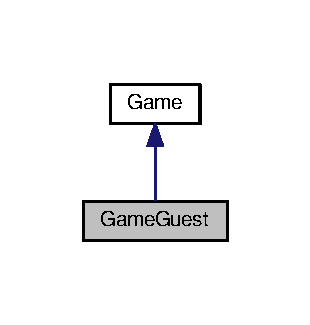
\includegraphics[width=149pt]{classMODEL_1_1GameGuest__inherit__graph}
\end{center}
\end{figure}


Collaboration diagram for Game\+Guest\+:\nopagebreak
\begin{figure}[H]
\begin{center}
\leavevmode
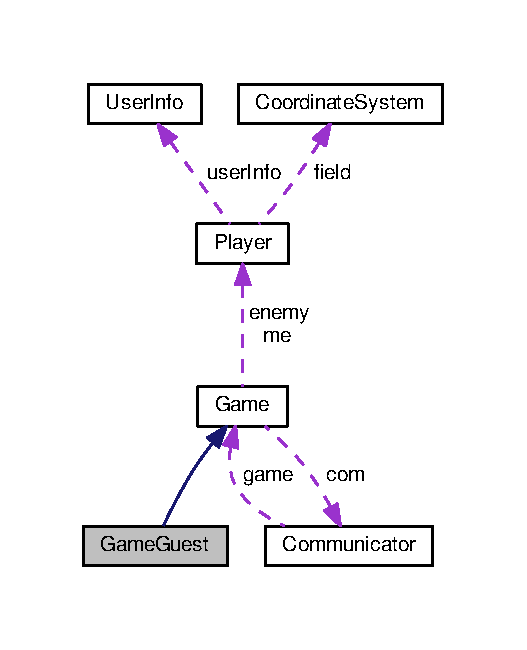
\includegraphics[width=253pt]{classMODEL_1_1GameGuest__coll__graph}
\end{center}
\end{figure}
\subsection*{Public Member Functions}
\begin{DoxyCompactItemize}
\item 
\hyperlink{classMODEL_1_1GameGuest_abd4b62394fc1e7d05395a049d3d4e57e}{Game\+Guest} (const std\+::string \&address, int port, std\+::vector$<$ std\+::reference\+\_\+wrapper$<$ \hyperlink{classBattleshipObserver}{Battleship\+Observer} $>$$>$ \&\hyperlink{classMODEL_1_1Game_afada2cb52f9872db4f3ab6e72d07cd05}{observer\+List}, \hyperlink{classUserInfo}{User\+Info} user\+Info)
\item 
\hyperlink{classMODEL_1_1GameGuest_a6df63e1b2db6ccf936d22495068755cb}{Game\+Guest} (\hyperlink{classMODEL_1_1GameGuest}{Game\+Guest} const \&)=delete
\item 
\hyperlink{classMODEL_1_1GameGuest}{Game\+Guest} \& \hyperlink{classMODEL_1_1GameGuest_ab61c4071b29d9c2c7fee6e919e20af66}{operator=} (\hyperlink{classMODEL_1_1GameGuest}{Game\+Guest} const \&other)=delete
\item 
\hyperlink{classMODEL_1_1GameGuest_a480d2bd3c04c585fa4e20e12394123b1}{Game\+Guest} (\hyperlink{classMODEL_1_1GameGuest}{Game\+Guest} \&\&other)=delete
\item 
\hyperlink{classMODEL_1_1GameGuest}{Game\+Guest} \& \hyperlink{classMODEL_1_1GameGuest_a8e2101bddf0da3dbb56279f2ddeecb5d}{operator=} (\hyperlink{classMODEL_1_1GameGuest}{Game\+Guest} \&\&other)=delete
\end{DoxyCompactItemize}
\subsection*{Additional Inherited Members}


\subsection{Detailed Description}
Inherits \hyperlink{classMODEL_1_1Game}{Game} and make it possible to manage guests game. 

\subsection{Constructor \& Destructor Documentation}
\index{M\+O\+D\+E\+L\+::\+Game\+Guest@{M\+O\+D\+E\+L\+::\+Game\+Guest}!Game\+Guest@{Game\+Guest}}
\index{Game\+Guest@{Game\+Guest}!M\+O\+D\+E\+L\+::\+Game\+Guest@{M\+O\+D\+E\+L\+::\+Game\+Guest}}
\subsubsection[{\texorpdfstring{Game\+Guest(const std\+::string \&address, int port, std\+::vector$<$ std\+::reference\+\_\+wrapper$<$ Battleship\+Observer $>$$>$ \&observer\+List, User\+Info user\+Info)}{GameGuest(const std::string &address, int port, std::vector< std::reference_wrapper< BattleshipObserver >> &observerList, UserInfo userInfo)}}]{\setlength{\rightskip}{0pt plus 5cm}{\bf Game\+Guest} (
\begin{DoxyParamCaption}
\item[{const std\+::string \&}]{address, }
\item[{int}]{port, }
\item[{std\+::vector$<$ std\+::reference\+\_\+wrapper$<$ {\bf Battleship\+Observer} $>$$>$ \&}]{observer\+List, }
\item[{{\bf User\+Info}}]{user\+Info}
\end{DoxyParamCaption}
)\hspace{0.3cm}{\ttfamily [explicit]}}\hypertarget{classMODEL_1_1GameGuest_abd4b62394fc1e7d05395a049d3d4e57e}{}\label{classMODEL_1_1GameGuest_abd4b62394fc1e7d05395a049d3d4e57e}
\index{M\+O\+D\+E\+L\+::\+Game\+Guest@{M\+O\+D\+E\+L\+::\+Game\+Guest}!Game\+Guest@{Game\+Guest}}
\index{Game\+Guest@{Game\+Guest}!M\+O\+D\+E\+L\+::\+Game\+Guest@{M\+O\+D\+E\+L\+::\+Game\+Guest}}
\subsubsection[{\texorpdfstring{Game\+Guest(\+Game\+Guest const \&)=delete}{GameGuest(GameGuest const &)=delete}}]{\setlength{\rightskip}{0pt plus 5cm}{\bf Game\+Guest} (
\begin{DoxyParamCaption}
\item[{{\bf Game\+Guest} const \&}]{}
\end{DoxyParamCaption}
)\hspace{0.3cm}{\ttfamily [delete]}}\hypertarget{classMODEL_1_1GameGuest_a6df63e1b2db6ccf936d22495068755cb}{}\label{classMODEL_1_1GameGuest_a6df63e1b2db6ccf936d22495068755cb}
\index{M\+O\+D\+E\+L\+::\+Game\+Guest@{M\+O\+D\+E\+L\+::\+Game\+Guest}!Game\+Guest@{Game\+Guest}}
\index{Game\+Guest@{Game\+Guest}!M\+O\+D\+E\+L\+::\+Game\+Guest@{M\+O\+D\+E\+L\+::\+Game\+Guest}}
\subsubsection[{\texorpdfstring{Game\+Guest(\+Game\+Guest \&\&other)=delete}{GameGuest(GameGuest &&other)=delete}}]{\setlength{\rightskip}{0pt plus 5cm}{\bf Game\+Guest} (
\begin{DoxyParamCaption}
\item[{{\bf Game\+Guest} \&\&}]{other}
\end{DoxyParamCaption}
)\hspace{0.3cm}{\ttfamily [delete]}}\hypertarget{classMODEL_1_1GameGuest_a480d2bd3c04c585fa4e20e12394123b1}{}\label{classMODEL_1_1GameGuest_a480d2bd3c04c585fa4e20e12394123b1}


\subsection{Member Function Documentation}
\index{M\+O\+D\+E\+L\+::\+Game\+Guest@{M\+O\+D\+E\+L\+::\+Game\+Guest}!operator=@{operator=}}
\index{operator=@{operator=}!M\+O\+D\+E\+L\+::\+Game\+Guest@{M\+O\+D\+E\+L\+::\+Game\+Guest}}
\subsubsection[{\texorpdfstring{operator=(\+Game\+Guest const \&other)=delete}{operator=(GameGuest const &other)=delete}}]{\setlength{\rightskip}{0pt plus 5cm}{\bf Game\+Guest}\& operator= (
\begin{DoxyParamCaption}
\item[{{\bf Game\+Guest} const \&}]{other}
\end{DoxyParamCaption}
)\hspace{0.3cm}{\ttfamily [delete]}}\hypertarget{classMODEL_1_1GameGuest_ab61c4071b29d9c2c7fee6e919e20af66}{}\label{classMODEL_1_1GameGuest_ab61c4071b29d9c2c7fee6e919e20af66}
\index{M\+O\+D\+E\+L\+::\+Game\+Guest@{M\+O\+D\+E\+L\+::\+Game\+Guest}!operator=@{operator=}}
\index{operator=@{operator=}!M\+O\+D\+E\+L\+::\+Game\+Guest@{M\+O\+D\+E\+L\+::\+Game\+Guest}}
\subsubsection[{\texorpdfstring{operator=(\+Game\+Guest \&\&other)=delete}{operator=(GameGuest &&other)=delete}}]{\setlength{\rightskip}{0pt plus 5cm}{\bf Game\+Guest}\& operator= (
\begin{DoxyParamCaption}
\item[{{\bf Game\+Guest} \&\&}]{other}
\end{DoxyParamCaption}
)\hspace{0.3cm}{\ttfamily [delete]}}\hypertarget{classMODEL_1_1GameGuest_a8e2101bddf0da3dbb56279f2ddeecb5d}{}\label{classMODEL_1_1GameGuest_a8e2101bddf0da3dbb56279f2ddeecb5d}


The documentation for this class was generated from the following files\+:\begin{DoxyCompactItemize}
\item 
model/\hyperlink{game__guest_8h}{game\+\_\+guest.\+h}\item 
model/\hyperlink{game__guest_8cpp}{game\+\_\+guest.\+cpp}\end{DoxyCompactItemize}

\hypertarget{classMODEL_1_1GameHost}{}\section{Game\+Host Class Reference}
\label{classMODEL_1_1GameHost}\index{Game\+Host@{Game\+Host}}


Inherits \hyperlink{classMODEL_1_1Game}{Game} and make it possible to manage hosts game.  




{\ttfamily \#include $<$game\+\_\+host.\+h$>$}



Inheritance diagram for Game\+Host\+:\nopagebreak
\begin{figure}[H]
\begin{center}
\leavevmode
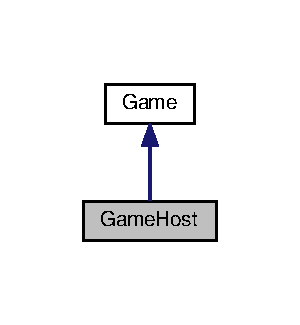
\includegraphics[width=144pt]{classMODEL_1_1GameHost__inherit__graph}
\end{center}
\end{figure}


Collaboration diagram for Game\+Host\+:\nopagebreak
\begin{figure}[H]
\begin{center}
\leavevmode
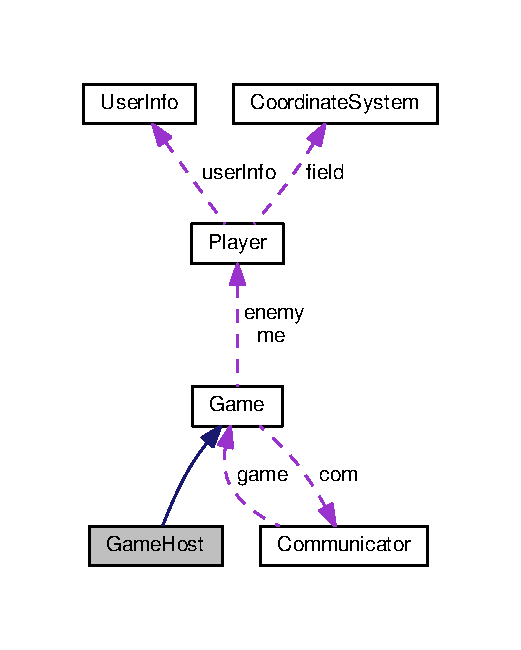
\includegraphics[width=250pt]{classMODEL_1_1GameHost__coll__graph}
\end{center}
\end{figure}
\subsection*{Public Member Functions}
\begin{DoxyCompactItemize}
\item 
\hyperlink{classMODEL_1_1GameHost_af4c7d7c228fb6a53529d42e5cf663454}{Game\+Host} (std\+::vector$<$ std\+::reference\+\_\+wrapper$<$ \hyperlink{classBattleshipObserver}{Battleship\+Observer} $>$$>$ \&\hyperlink{classMODEL_1_1Game_afada2cb52f9872db4f3ab6e72d07cd05}{observer\+List}, \hyperlink{classUserInfo}{User\+Info} user\+Info)
\item 
\hyperlink{classMODEL_1_1GameHost_a80f71e5ed2203e72e6316cd576f34b20}{Game\+Host} (\hyperlink{classMODEL_1_1GameHost}{Game\+Host} const \&)=delete
\item 
\hyperlink{classMODEL_1_1GameHost}{Game\+Host} \& \hyperlink{classMODEL_1_1GameHost_a0ea4d71078c853546b5e20eb4456c52c}{operator=} (\hyperlink{classMODEL_1_1GameHost}{Game\+Host} const \&other)=delete
\item 
\hyperlink{classMODEL_1_1GameHost_a2f8ceef0f550ba2a56d02634eba1e578}{Game\+Host} (\hyperlink{classMODEL_1_1GameHost}{Game\+Host} \&\&other)=delete
\item 
\hyperlink{classMODEL_1_1GameHost}{Game\+Host} \& \hyperlink{classMODEL_1_1GameHost_a9e001ceb501503e01025415889d8e3a1}{operator=} (\hyperlink{classMODEL_1_1GameHost}{Game\+Host} \&\&other)=delete
\end{DoxyCompactItemize}
\subsection*{Additional Inherited Members}


\subsection{Detailed Description}
Inherits \hyperlink{classMODEL_1_1Game}{Game} and make it possible to manage hosts game. 

\subsection{Constructor \& Destructor Documentation}
\index{M\+O\+D\+E\+L\+::\+Game\+Host@{M\+O\+D\+E\+L\+::\+Game\+Host}!Game\+Host@{Game\+Host}}
\index{Game\+Host@{Game\+Host}!M\+O\+D\+E\+L\+::\+Game\+Host@{M\+O\+D\+E\+L\+::\+Game\+Host}}
\subsubsection[{\texorpdfstring{Game\+Host(std\+::vector$<$ std\+::reference\+\_\+wrapper$<$ Battleship\+Observer $>$$>$ \&observer\+List, User\+Info user\+Info)}{GameHost(std::vector< std::reference_wrapper< BattleshipObserver >> &observerList, UserInfo userInfo)}}]{\setlength{\rightskip}{0pt plus 5cm}{\bf Game\+Host} (
\begin{DoxyParamCaption}
\item[{std\+::vector$<$ std\+::reference\+\_\+wrapper$<$ {\bf Battleship\+Observer} $>$$>$ \&}]{observer\+List, }
\item[{{\bf User\+Info}}]{user\+Info}
\end{DoxyParamCaption}
)}\hypertarget{classMODEL_1_1GameHost_af4c7d7c228fb6a53529d42e5cf663454}{}\label{classMODEL_1_1GameHost_af4c7d7c228fb6a53529d42e5cf663454}
\index{M\+O\+D\+E\+L\+::\+Game\+Host@{M\+O\+D\+E\+L\+::\+Game\+Host}!Game\+Host@{Game\+Host}}
\index{Game\+Host@{Game\+Host}!M\+O\+D\+E\+L\+::\+Game\+Host@{M\+O\+D\+E\+L\+::\+Game\+Host}}
\subsubsection[{\texorpdfstring{Game\+Host(\+Game\+Host const \&)=delete}{GameHost(GameHost const &)=delete}}]{\setlength{\rightskip}{0pt plus 5cm}{\bf Game\+Host} (
\begin{DoxyParamCaption}
\item[{{\bf Game\+Host} const \&}]{}
\end{DoxyParamCaption}
)\hspace{0.3cm}{\ttfamily [delete]}}\hypertarget{classMODEL_1_1GameHost_a80f71e5ed2203e72e6316cd576f34b20}{}\label{classMODEL_1_1GameHost_a80f71e5ed2203e72e6316cd576f34b20}
\index{M\+O\+D\+E\+L\+::\+Game\+Host@{M\+O\+D\+E\+L\+::\+Game\+Host}!Game\+Host@{Game\+Host}}
\index{Game\+Host@{Game\+Host}!M\+O\+D\+E\+L\+::\+Game\+Host@{M\+O\+D\+E\+L\+::\+Game\+Host}}
\subsubsection[{\texorpdfstring{Game\+Host(\+Game\+Host \&\&other)=delete}{GameHost(GameHost &&other)=delete}}]{\setlength{\rightskip}{0pt plus 5cm}{\bf Game\+Host} (
\begin{DoxyParamCaption}
\item[{{\bf Game\+Host} \&\&}]{other}
\end{DoxyParamCaption}
)\hspace{0.3cm}{\ttfamily [delete]}}\hypertarget{classMODEL_1_1GameHost_a2f8ceef0f550ba2a56d02634eba1e578}{}\label{classMODEL_1_1GameHost_a2f8ceef0f550ba2a56d02634eba1e578}


\subsection{Member Function Documentation}
\index{M\+O\+D\+E\+L\+::\+Game\+Host@{M\+O\+D\+E\+L\+::\+Game\+Host}!operator=@{operator=}}
\index{operator=@{operator=}!M\+O\+D\+E\+L\+::\+Game\+Host@{M\+O\+D\+E\+L\+::\+Game\+Host}}
\subsubsection[{\texorpdfstring{operator=(\+Game\+Host const \&other)=delete}{operator=(GameHost const &other)=delete}}]{\setlength{\rightskip}{0pt plus 5cm}{\bf Game\+Host}\& operator= (
\begin{DoxyParamCaption}
\item[{{\bf Game\+Host} const \&}]{other}
\end{DoxyParamCaption}
)\hspace{0.3cm}{\ttfamily [delete]}}\hypertarget{classMODEL_1_1GameHost_a0ea4d71078c853546b5e20eb4456c52c}{}\label{classMODEL_1_1GameHost_a0ea4d71078c853546b5e20eb4456c52c}
\index{M\+O\+D\+E\+L\+::\+Game\+Host@{M\+O\+D\+E\+L\+::\+Game\+Host}!operator=@{operator=}}
\index{operator=@{operator=}!M\+O\+D\+E\+L\+::\+Game\+Host@{M\+O\+D\+E\+L\+::\+Game\+Host}}
\subsubsection[{\texorpdfstring{operator=(\+Game\+Host \&\&other)=delete}{operator=(GameHost &&other)=delete}}]{\setlength{\rightskip}{0pt plus 5cm}{\bf Game\+Host}\& operator= (
\begin{DoxyParamCaption}
\item[{{\bf Game\+Host} \&\&}]{other}
\end{DoxyParamCaption}
)\hspace{0.3cm}{\ttfamily [delete]}}\hypertarget{classMODEL_1_1GameHost_a9e001ceb501503e01025415889d8e3a1}{}\label{classMODEL_1_1GameHost_a9e001ceb501503e01025415889d8e3a1}


The documentation for this class was generated from the following files\+:\begin{DoxyCompactItemize}
\item 
model/\hyperlink{game__host_8h}{game\+\_\+host.\+h}\item 
model/\hyperlink{game__host_8cpp}{game\+\_\+host.\+cpp}\end{DoxyCompactItemize}

\hypertarget{classModelInterface}{}\section{Model\+Interface Class Reference}
\label{classModelInterface}\index{Model\+Interface@{Model\+Interface}}


The base class that defines the model interface.  




{\ttfamily \#include $<$model\+\_\+interface.\+h$>$}



Inheritance diagram for Model\+Interface\+:\nopagebreak
\begin{figure}[H]
\begin{center}
\leavevmode
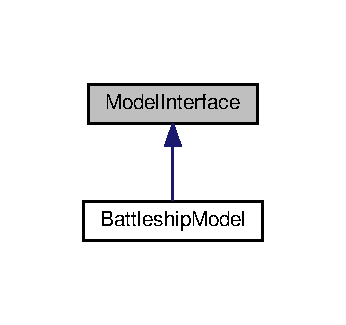
\includegraphics[width=166pt]{classModelInterface__inherit__graph}
\end{center}
\end{figure}
\subsection*{Public Member Functions}
\begin{DoxyCompactItemize}
\item 
virtual \hyperlink{classModelInterface_a185a78e2f43b18782afa624cedb412fc}{$\sim$\+Model\+Interface} ()
\item 
virtual void \hyperlink{classModelInterface_a38d9c2d3c1b09f40910a7ad1aa1aace4}{register\+Observer} (\hyperlink{classBattleshipObserver}{Battleship\+Observer} \&observer)=0
\item 
virtual void \hyperlink{classModelInterface_a36aeb8e4e01dd08fd0416f3269789b31}{start\+New\+Game\+As\+Host} (\hyperlink{classUserInfo}{User\+Info} user\+Info)=0
\item 
virtual void \hyperlink{classModelInterface_aee662ec9439a2344dcd39a0b65dcf639}{start\+New\+Game\+As\+Guest} (const std\+::string \&address, int port, \hyperlink{classUserInfo}{User\+Info} user\+Info)=0
\item 
virtual void \hyperlink{classModelInterface_a2bb725b2837f07c50718296b2acb9bd6}{cancel\+Hosting} ()=0
\item 
virtual void \hyperlink{classModelInterface_aa708cd5411011ade34c2796b3f102612}{place\+Ship} (\hyperlink{classMODEL_1_1Point}{M\+O\+D\+E\+L\+::\+Point} p1, \hyperlink{classMODEL_1_1Point}{M\+O\+D\+E\+L\+::\+Point} p2)=0
\end{DoxyCompactItemize}


\subsection{Detailed Description}
The base class that defines the model interface. 

\subsection{Constructor \& Destructor Documentation}
\index{Model\+Interface@{Model\+Interface}!````~Model\+Interface@{$\sim$\+Model\+Interface}}
\index{````~Model\+Interface@{$\sim$\+Model\+Interface}!Model\+Interface@{Model\+Interface}}
\subsubsection[{\texorpdfstring{$\sim$\+Model\+Interface()}{~ModelInterface()}}]{\setlength{\rightskip}{0pt plus 5cm}virtual $\sim${\bf Model\+Interface} (
\begin{DoxyParamCaption}
{}
\end{DoxyParamCaption}
)\hspace{0.3cm}{\ttfamily [inline]}, {\ttfamily [virtual]}}\hypertarget{classModelInterface_a185a78e2f43b18782afa624cedb412fc}{}\label{classModelInterface_a185a78e2f43b18782afa624cedb412fc}


\subsection{Member Function Documentation}
\index{Model\+Interface@{Model\+Interface}!cancel\+Hosting@{cancel\+Hosting}}
\index{cancel\+Hosting@{cancel\+Hosting}!Model\+Interface@{Model\+Interface}}
\subsubsection[{\texorpdfstring{cancel\+Hosting()=0}{cancelHosting()=0}}]{\setlength{\rightskip}{0pt plus 5cm}virtual void cancel\+Hosting (
\begin{DoxyParamCaption}
{}
\end{DoxyParamCaption}
)\hspace{0.3cm}{\ttfamily [pure virtual]}}\hypertarget{classModelInterface_a2bb725b2837f07c50718296b2acb9bd6}{}\label{classModelInterface_a2bb725b2837f07c50718296b2acb9bd6}
user can stop while hosting game and waiting for others to join his game. This is the case after Model\+Interface\+::start\+New\+Game\+As\+Host(const std\+::string\&, int) call 

Implemented in \hyperlink{classMODEL_1_1BattleshipModel_aa7cd87fbe771e195626f19960095bded}{Battleship\+Model}.

\index{Model\+Interface@{Model\+Interface}!place\+Ship@{place\+Ship}}
\index{place\+Ship@{place\+Ship}!Model\+Interface@{Model\+Interface}}
\subsubsection[{\texorpdfstring{place\+Ship(\+M\+O\+D\+E\+L\+::\+Point p1, M\+O\+D\+E\+L\+::\+Point p2)=0}{placeShip(MODEL::Point p1, MODEL::Point p2)=0}}]{\setlength{\rightskip}{0pt plus 5cm}virtual void place\+Ship (
\begin{DoxyParamCaption}
\item[{{\bf M\+O\+D\+E\+L\+::\+Point}}]{p1, }
\item[{{\bf M\+O\+D\+E\+L\+::\+Point}}]{p2}
\end{DoxyParamCaption}
)\hspace{0.3cm}{\ttfamily [pure virtual]}}\hypertarget{classModelInterface_aa708cd5411011ade34c2796b3f102612}{}\label{classModelInterface_aa708cd5411011ade34c2796b3f102612}

\begin{DoxyExceptions}{Exceptions}
{\em std\+::length\+\_\+error} & if ship count exceeds 5. \\
\hline
\end{DoxyExceptions}


Implemented in \hyperlink{classMODEL_1_1BattleshipModel_a6de4c3b25683e4774fc9b524aa8c7e6a}{Battleship\+Model}.

\index{Model\+Interface@{Model\+Interface}!register\+Observer@{register\+Observer}}
\index{register\+Observer@{register\+Observer}!Model\+Interface@{Model\+Interface}}
\subsubsection[{\texorpdfstring{register\+Observer(\+Battleship\+Observer \&observer)=0}{registerObserver(BattleshipObserver &observer)=0}}]{\setlength{\rightskip}{0pt plus 5cm}virtual void register\+Observer (
\begin{DoxyParamCaption}
\item[{{\bf Battleship\+Observer} \&}]{observer}
\end{DoxyParamCaption}
)\hspace{0.3cm}{\ttfamily [pure virtual]}}\hypertarget{classModelInterface_a38d9c2d3c1b09f40910a7ad1aa1aace4}{}\label{classModelInterface_a38d9c2d3c1b09f40910a7ad1aa1aace4}
Observer pattern as a part of M\+V\+C-\/\+Pattern 
\begin{DoxyParams}{Parameters}
{\em observer} & is usally a gui, that reflects/shows state-\/changes of the model \\
\hline
\end{DoxyParams}


Implemented in \hyperlink{classMODEL_1_1BattleshipModel_a1afa557183362f561ae105fa141941ea}{Battleship\+Model}.

\index{Model\+Interface@{Model\+Interface}!start\+New\+Game\+As\+Guest@{start\+New\+Game\+As\+Guest}}
\index{start\+New\+Game\+As\+Guest@{start\+New\+Game\+As\+Guest}!Model\+Interface@{Model\+Interface}}
\subsubsection[{\texorpdfstring{start\+New\+Game\+As\+Guest(const std\+::string \&address, int port, User\+Info user\+Info)=0}{startNewGameAsGuest(const std::string &address, int port, UserInfo userInfo)=0}}]{\setlength{\rightskip}{0pt plus 5cm}virtual void start\+New\+Game\+As\+Guest (
\begin{DoxyParamCaption}
\item[{const std\+::string \&}]{address, }
\item[{int}]{port, }
\item[{{\bf User\+Info}}]{user\+Info}
\end{DoxyParamCaption}
)\hspace{0.3cm}{\ttfamily [pure virtual]}}\hypertarget{classModelInterface_aee662ec9439a2344dcd39a0b65dcf639}{}\label{classModelInterface_aee662ec9439a2344dcd39a0b65dcf639}
connect to a host as a guest over the network 
\begin{DoxyParams}{Parameters}
{\em address} & ipv4 address \\
\hline
{\em port} & a port number \\
\hline
{\em player\+Name} & a name, like firstname \\
\hline
{\em age} & biological age of a human player \\
\hline
\end{DoxyParams}


Implemented in \hyperlink{classMODEL_1_1BattleshipModel_a076ef235e6ff9708c2bc0c2a4dcc141b}{Battleship\+Model}.

\index{Model\+Interface@{Model\+Interface}!start\+New\+Game\+As\+Host@{start\+New\+Game\+As\+Host}}
\index{start\+New\+Game\+As\+Host@{start\+New\+Game\+As\+Host}!Model\+Interface@{Model\+Interface}}
\subsubsection[{\texorpdfstring{start\+New\+Game\+As\+Host(\+User\+Info user\+Info)=0}{startNewGameAsHost(UserInfo userInfo)=0}}]{\setlength{\rightskip}{0pt plus 5cm}virtual void start\+New\+Game\+As\+Host (
\begin{DoxyParamCaption}
\item[{{\bf User\+Info}}]{user\+Info}
\end{DoxyParamCaption}
)\hspace{0.3cm}{\ttfamily [pure virtual]}}\hypertarget{classModelInterface_a36aeb8e4e01dd08fd0416f3269789b31}{}\label{classModelInterface_a36aeb8e4e01dd08fd0416f3269789b31}
begin new game as host over the network. But first wat for guest to join. 

Implemented in \hyperlink{classMODEL_1_1BattleshipModel_a655da28525f6ac4d2d15da6808c538b9}{Battleship\+Model}.



The documentation for this class was generated from the following file\+:\begin{DoxyCompactItemize}
\item 
common/\hyperlink{model__interface_8h}{model\+\_\+interface.\+h}\end{DoxyCompactItemize}

\hypertarget{classModelTest}{}\section{Model\+Test Class Reference}
\label{classModelTest}\index{Model\+Test@{Model\+Test}}


Inheritance diagram for Model\+Test\+:\nopagebreak
\begin{figure}[H]
\begin{center}
\leavevmode
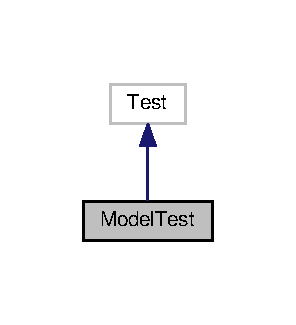
\includegraphics[width=142pt]{classModelTest__inherit__graph}
\end{center}
\end{figure}


Collaboration diagram for Model\+Test\+:\nopagebreak
\begin{figure}[H]
\begin{center}
\leavevmode
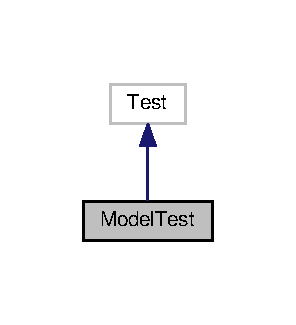
\includegraphics[width=142pt]{classModelTest__coll__graph}
\end{center}
\end{figure}
\subsection*{Protected Member Functions}
\begin{DoxyCompactItemize}
\item 
\hyperlink{classModelTest_a79c9529463b64a538e65b324fa61de9f}{Model\+Test} ()
\item 
virtual \hyperlink{classModelTest_a139b48c7352777a2732a72fc61b46735}{$\sim$\+Model\+Test} ()
\item 
virtual void \hyperlink{classModelTest_a901706a587f9ae84df8b2395fbe759cb}{Set\+Up} ()
\item 
virtual void \hyperlink{classModelTest_a870a092058305911f3d42df45dd657e5}{Tear\+Down} ()
\end{DoxyCompactItemize}


\subsection{Constructor \& Destructor Documentation}
\index{Model\+Test@{Model\+Test}!Model\+Test@{Model\+Test}}
\index{Model\+Test@{Model\+Test}!Model\+Test@{Model\+Test}}
\subsubsection[{\texorpdfstring{Model\+Test()}{ModelTest()}}]{\setlength{\rightskip}{0pt plus 5cm}{\bf Model\+Test} (
\begin{DoxyParamCaption}
{}
\end{DoxyParamCaption}
)\hspace{0.3cm}{\ttfamily [inline]}, {\ttfamily [protected]}}\hypertarget{classModelTest_a79c9529463b64a538e65b324fa61de9f}{}\label{classModelTest_a79c9529463b64a538e65b324fa61de9f}
\index{Model\+Test@{Model\+Test}!````~Model\+Test@{$\sim$\+Model\+Test}}
\index{````~Model\+Test@{$\sim$\+Model\+Test}!Model\+Test@{Model\+Test}}
\subsubsection[{\texorpdfstring{$\sim$\+Model\+Test()}{~ModelTest()}}]{\setlength{\rightskip}{0pt plus 5cm}virtual $\sim${\bf Model\+Test} (
\begin{DoxyParamCaption}
{}
\end{DoxyParamCaption}
)\hspace{0.3cm}{\ttfamily [inline]}, {\ttfamily [protected]}, {\ttfamily [virtual]}}\hypertarget{classModelTest_a139b48c7352777a2732a72fc61b46735}{}\label{classModelTest_a139b48c7352777a2732a72fc61b46735}


\subsection{Member Function Documentation}
\index{Model\+Test@{Model\+Test}!Set\+Up@{Set\+Up}}
\index{Set\+Up@{Set\+Up}!Model\+Test@{Model\+Test}}
\subsubsection[{\texorpdfstring{Set\+Up()}{SetUp()}}]{\setlength{\rightskip}{0pt plus 5cm}virtual void Set\+Up (
\begin{DoxyParamCaption}
{}
\end{DoxyParamCaption}
)\hspace{0.3cm}{\ttfamily [inline]}, {\ttfamily [protected]}, {\ttfamily [virtual]}}\hypertarget{classModelTest_a901706a587f9ae84df8b2395fbe759cb}{}\label{classModelTest_a901706a587f9ae84df8b2395fbe759cb}
\index{Model\+Test@{Model\+Test}!Tear\+Down@{Tear\+Down}}
\index{Tear\+Down@{Tear\+Down}!Model\+Test@{Model\+Test}}
\subsubsection[{\texorpdfstring{Tear\+Down()}{TearDown()}}]{\setlength{\rightskip}{0pt plus 5cm}virtual void Tear\+Down (
\begin{DoxyParamCaption}
{}
\end{DoxyParamCaption}
)\hspace{0.3cm}{\ttfamily [inline]}, {\ttfamily [protected]}, {\ttfamily [virtual]}}\hypertarget{classModelTest_a870a092058305911f3d42df45dd657e5}{}\label{classModelTest_a870a092058305911f3d42df45dd657e5}


The documentation for this class was generated from the following file\+:\begin{DoxyCompactItemize}
\item 
\hyperlink{test__model_8cpp}{test\+\_\+model.\+cpp}\end{DoxyCompactItemize}

\hypertarget{classPlayer}{}\section{Player Class Reference}
\label{classPlayer}\index{Player@{Player}}


A class representing player for graphical interface.  




{\ttfamily \#include $<$player.\+h$>$}

\subsection*{Public Member Functions}
\begin{DoxyCompactItemize}
\item 
\hyperlink{classPlayer_aa862d30723707ac0ce1923d103a5033f}{Player} (Q\+String $\ast$name\+Player, int age\+Player)
\item 
void \hyperlink{classPlayer_a0c1485a5850d704d9b373ebe21cb9b21}{set\+Name} (Q\+String $\ast$name\+Player)
\item 
Q\+String $\ast$ \hyperlink{classPlayer_ae3585f991fe37695e2b1a5eba8cacac1}{get\+Name} ()
\item 
void \hyperlink{classPlayer_a23e901febda7a2f14791b3557c247df0}{set\+Age} (int \hyperlink{classPlayer_a91d98a856bbd96810b40af3ca5cc901a}{age})
\item 
int \hyperlink{classPlayer_a44a88871339022e9a268d613b55f39a1}{get\+Age} ()
\item 
void \hyperlink{classPlayer_a15e6f02e21348714fabfa32c176e2b4b}{set\+Number\+Wins} (int \hyperlink{classPlayer_a5490bb5e66c3e5ac702c7df4f363d57d}{number\+Wins})
\item 
int \hyperlink{classPlayer_ab4b4189b22c7952d961060550146a5e3}{get\+Number\+Wins} ()
\item 
void \hyperlink{classPlayer_aedf3ee71765e18407ad4ba30a8d25d4b}{set\+Number\+Games} (int \hyperlink{classPlayer_a1d6d057cd152c5d158546791cbd6bc8f}{number\+Games})
\item 
int \hyperlink{classPlayer_a1bcc25b1f0cb70eec57316d4bee68359}{get\+Number\+Games} ()
\item 
void \hyperlink{classPlayer_aaa363c802f56d43e77f1276b9851b5a5}{set\+Number\+Failures} (int number\+Failure)
\item 
int \hyperlink{classPlayer_a8b87716141c31266b5bb5ba5372b9b64}{get\+Number\+Failures} ()
\item 
void \hyperlink{classPlayer_a2a94b5f95dfbe0d2b19f925eec316a1d}{set\+Grade} (int \hyperlink{classPlayer_a13d4b9fff7f9b28844a348b444cff7be}{grade})
\item 
int \hyperlink{classPlayer_a8320479b8d8233a1f9e97db652d228e9}{get\+Grade} ()
\item 
void \hyperlink{classPlayer_a37db9063f0dd514f2dc74a20fb4f5b71}{change\+Profile} (Q\+String $\ast$name\+Player, int \hyperlink{classPlayer_a91d98a856bbd96810b40af3ca5cc901a}{age})
\item 
Q\+String $\ast$ \hyperlink{classPlayer_aa4991dab5d59dfd37e9da17465e8dc52}{get\+Stats} ()
\item 
void \hyperlink{classPlayer_a67f249eb58bec9270d90245a97211d52}{add\+Last\+Oponent} (Q\+String recent\+Oponents)
\item 
Q\+List$<$ Q\+String $>$ \hyperlink{classPlayer_a6e0c06b360697a7f3fea19e5e1de37c3}{get\+Last\+Oponents} ()
\end{DoxyCompactItemize}
\subsection*{Private Attributes}
\begin{DoxyCompactItemize}
\item 
Q\+String $\ast$ \hyperlink{classPlayer_a4b7508f4b75dd810016635bb8a9ee1e3}{name}
\item 
int \hyperlink{classPlayer_a91d98a856bbd96810b40af3ca5cc901a}{age}
\item 
int \hyperlink{classPlayer_a1d6d057cd152c5d158546791cbd6bc8f}{number\+Games} = 0
\item 
int \hyperlink{classPlayer_a5490bb5e66c3e5ac702c7df4f363d57d}{number\+Wins} = 0
\item 
int \hyperlink{classPlayer_aeee09fe6d2b453144787ac2b70052d69}{number\+Failures} = 0
\item 
int \hyperlink{classPlayer_a13d4b9fff7f9b28844a348b444cff7be}{grade} = 0
\item 
Q\+List$<$ Q\+String $>$ \hyperlink{classPlayer_aa26e1577cdda5a121a83a7fb5dd4c985}{last\+Oponents}
\end{DoxyCompactItemize}


\subsection{Detailed Description}
A class representing player for graphical interface. 

\subsection{Constructor \& Destructor Documentation}
\index{Player@{Player}!Player@{Player}}
\index{Player@{Player}!Player@{Player}}
\subsubsection[{\texorpdfstring{Player(\+Q\+String $\ast$name\+Player, int age\+Player)}{Player(QString *namePlayer, int agePlayer)}}]{\setlength{\rightskip}{0pt plus 5cm}{\bf Player} (
\begin{DoxyParamCaption}
\item[{Q\+String $\ast$}]{name\+Player, }
\item[{int}]{age\+Player}
\end{DoxyParamCaption}
)}\hypertarget{classPlayer_aa862d30723707ac0ce1923d103a5033f}{}\label{classPlayer_aa862d30723707ac0ce1923d103a5033f}


\subsection{Member Function Documentation}
\index{Player@{Player}!add\+Last\+Oponent@{add\+Last\+Oponent}}
\index{add\+Last\+Oponent@{add\+Last\+Oponent}!Player@{Player}}
\subsubsection[{\texorpdfstring{add\+Last\+Oponent(\+Q\+String recent\+Oponents)}{addLastOponent(QString recentOponents)}}]{\setlength{\rightskip}{0pt plus 5cm}void add\+Last\+Oponent (
\begin{DoxyParamCaption}
\item[{Q\+String}]{recent\+Oponents}
\end{DoxyParamCaption}
)}\hypertarget{classPlayer_a67f249eb58bec9270d90245a97211d52}{}\label{classPlayer_a67f249eb58bec9270d90245a97211d52}
\index{Player@{Player}!change\+Profile@{change\+Profile}}
\index{change\+Profile@{change\+Profile}!Player@{Player}}
\subsubsection[{\texorpdfstring{change\+Profile(\+Q\+String $\ast$name\+Player, int age)}{changeProfile(QString *namePlayer, int age)}}]{\setlength{\rightskip}{0pt plus 5cm}void change\+Profile (
\begin{DoxyParamCaption}
\item[{Q\+String $\ast$}]{name\+Player, }
\item[{int}]{age}
\end{DoxyParamCaption}
)}\hypertarget{classPlayer_a37db9063f0dd514f2dc74a20fb4f5b71}{}\label{classPlayer_a37db9063f0dd514f2dc74a20fb4f5b71}
\index{Player@{Player}!get\+Age@{get\+Age}}
\index{get\+Age@{get\+Age}!Player@{Player}}
\subsubsection[{\texorpdfstring{get\+Age()}{getAge()}}]{\setlength{\rightskip}{0pt plus 5cm}int get\+Age (
\begin{DoxyParamCaption}
{}
\end{DoxyParamCaption}
)}\hypertarget{classPlayer_a44a88871339022e9a268d613b55f39a1}{}\label{classPlayer_a44a88871339022e9a268d613b55f39a1}
\index{Player@{Player}!get\+Grade@{get\+Grade}}
\index{get\+Grade@{get\+Grade}!Player@{Player}}
\subsubsection[{\texorpdfstring{get\+Grade()}{getGrade()}}]{\setlength{\rightskip}{0pt plus 5cm}int get\+Grade (
\begin{DoxyParamCaption}
{}
\end{DoxyParamCaption}
)}\hypertarget{classPlayer_a8320479b8d8233a1f9e97db652d228e9}{}\label{classPlayer_a8320479b8d8233a1f9e97db652d228e9}
\index{Player@{Player}!get\+Last\+Oponents@{get\+Last\+Oponents}}
\index{get\+Last\+Oponents@{get\+Last\+Oponents}!Player@{Player}}
\subsubsection[{\texorpdfstring{get\+Last\+Oponents()}{getLastOponents()}}]{\setlength{\rightskip}{0pt plus 5cm}Q\+List$<$ Q\+String $>$ get\+Last\+Oponents (
\begin{DoxyParamCaption}
{}
\end{DoxyParamCaption}
)}\hypertarget{classPlayer_a6e0c06b360697a7f3fea19e5e1de37c3}{}\label{classPlayer_a6e0c06b360697a7f3fea19e5e1de37c3}
\index{Player@{Player}!get\+Name@{get\+Name}}
\index{get\+Name@{get\+Name}!Player@{Player}}
\subsubsection[{\texorpdfstring{get\+Name()}{getName()}}]{\setlength{\rightskip}{0pt plus 5cm}Q\+String $\ast$ get\+Name (
\begin{DoxyParamCaption}
{}
\end{DoxyParamCaption}
)}\hypertarget{classPlayer_ae3585f991fe37695e2b1a5eba8cacac1}{}\label{classPlayer_ae3585f991fe37695e2b1a5eba8cacac1}
\index{Player@{Player}!get\+Number\+Failures@{get\+Number\+Failures}}
\index{get\+Number\+Failures@{get\+Number\+Failures}!Player@{Player}}
\subsubsection[{\texorpdfstring{get\+Number\+Failures()}{getNumberFailures()}}]{\setlength{\rightskip}{0pt plus 5cm}int get\+Number\+Failures (
\begin{DoxyParamCaption}
{}
\end{DoxyParamCaption}
)}\hypertarget{classPlayer_a8b87716141c31266b5bb5ba5372b9b64}{}\label{classPlayer_a8b87716141c31266b5bb5ba5372b9b64}
\index{Player@{Player}!get\+Number\+Games@{get\+Number\+Games}}
\index{get\+Number\+Games@{get\+Number\+Games}!Player@{Player}}
\subsubsection[{\texorpdfstring{get\+Number\+Games()}{getNumberGames()}}]{\setlength{\rightskip}{0pt plus 5cm}int get\+Number\+Games (
\begin{DoxyParamCaption}
{}
\end{DoxyParamCaption}
)}\hypertarget{classPlayer_a1bcc25b1f0cb70eec57316d4bee68359}{}\label{classPlayer_a1bcc25b1f0cb70eec57316d4bee68359}
\index{Player@{Player}!get\+Number\+Wins@{get\+Number\+Wins}}
\index{get\+Number\+Wins@{get\+Number\+Wins}!Player@{Player}}
\subsubsection[{\texorpdfstring{get\+Number\+Wins()}{getNumberWins()}}]{\setlength{\rightskip}{0pt plus 5cm}int get\+Number\+Wins (
\begin{DoxyParamCaption}
{}
\end{DoxyParamCaption}
)}\hypertarget{classPlayer_ab4b4189b22c7952d961060550146a5e3}{}\label{classPlayer_ab4b4189b22c7952d961060550146a5e3}
\index{Player@{Player}!get\+Stats@{get\+Stats}}
\index{get\+Stats@{get\+Stats}!Player@{Player}}
\subsubsection[{\texorpdfstring{get\+Stats()}{getStats()}}]{\setlength{\rightskip}{0pt plus 5cm}Q\+String $\ast$ get\+Stats (
\begin{DoxyParamCaption}
{}
\end{DoxyParamCaption}
)}\hypertarget{classPlayer_aa4991dab5d59dfd37e9da17465e8dc52}{}\label{classPlayer_aa4991dab5d59dfd37e9da17465e8dc52}
\index{Player@{Player}!set\+Age@{set\+Age}}
\index{set\+Age@{set\+Age}!Player@{Player}}
\subsubsection[{\texorpdfstring{set\+Age(int age)}{setAge(int age)}}]{\setlength{\rightskip}{0pt plus 5cm}void set\+Age (
\begin{DoxyParamCaption}
\item[{int}]{age}
\end{DoxyParamCaption}
)}\hypertarget{classPlayer_a23e901febda7a2f14791b3557c247df0}{}\label{classPlayer_a23e901febda7a2f14791b3557c247df0}
\index{Player@{Player}!set\+Grade@{set\+Grade}}
\index{set\+Grade@{set\+Grade}!Player@{Player}}
\subsubsection[{\texorpdfstring{set\+Grade(int grade)}{setGrade(int grade)}}]{\setlength{\rightskip}{0pt plus 5cm}void set\+Grade (
\begin{DoxyParamCaption}
\item[{int}]{grade}
\end{DoxyParamCaption}
)}\hypertarget{classPlayer_a2a94b5f95dfbe0d2b19f925eec316a1d}{}\label{classPlayer_a2a94b5f95dfbe0d2b19f925eec316a1d}
\index{Player@{Player}!set\+Name@{set\+Name}}
\index{set\+Name@{set\+Name}!Player@{Player}}
\subsubsection[{\texorpdfstring{set\+Name(\+Q\+String $\ast$name\+Player)}{setName(QString *namePlayer)}}]{\setlength{\rightskip}{0pt plus 5cm}void set\+Name (
\begin{DoxyParamCaption}
\item[{Q\+String $\ast$}]{name\+Player}
\end{DoxyParamCaption}
)}\hypertarget{classPlayer_a0c1485a5850d704d9b373ebe21cb9b21}{}\label{classPlayer_a0c1485a5850d704d9b373ebe21cb9b21}
\index{Player@{Player}!set\+Number\+Failures@{set\+Number\+Failures}}
\index{set\+Number\+Failures@{set\+Number\+Failures}!Player@{Player}}
\subsubsection[{\texorpdfstring{set\+Number\+Failures(int number\+Failure)}{setNumberFailures(int numberFailure)}}]{\setlength{\rightskip}{0pt plus 5cm}void set\+Number\+Failures (
\begin{DoxyParamCaption}
\item[{int}]{number\+Failure}
\end{DoxyParamCaption}
)}\hypertarget{classPlayer_aaa363c802f56d43e77f1276b9851b5a5}{}\label{classPlayer_aaa363c802f56d43e77f1276b9851b5a5}
\index{Player@{Player}!set\+Number\+Games@{set\+Number\+Games}}
\index{set\+Number\+Games@{set\+Number\+Games}!Player@{Player}}
\subsubsection[{\texorpdfstring{set\+Number\+Games(int number\+Games)}{setNumberGames(int numberGames)}}]{\setlength{\rightskip}{0pt plus 5cm}void set\+Number\+Games (
\begin{DoxyParamCaption}
\item[{int}]{number\+Games}
\end{DoxyParamCaption}
)}\hypertarget{classPlayer_aedf3ee71765e18407ad4ba30a8d25d4b}{}\label{classPlayer_aedf3ee71765e18407ad4ba30a8d25d4b}
\index{Player@{Player}!set\+Number\+Wins@{set\+Number\+Wins}}
\index{set\+Number\+Wins@{set\+Number\+Wins}!Player@{Player}}
\subsubsection[{\texorpdfstring{set\+Number\+Wins(int number\+Wins)}{setNumberWins(int numberWins)}}]{\setlength{\rightskip}{0pt plus 5cm}void set\+Number\+Wins (
\begin{DoxyParamCaption}
\item[{int}]{number\+Wins}
\end{DoxyParamCaption}
)}\hypertarget{classPlayer_a15e6f02e21348714fabfa32c176e2b4b}{}\label{classPlayer_a15e6f02e21348714fabfa32c176e2b4b}


\subsection{Member Data Documentation}
\index{Player@{Player}!age@{age}}
\index{age@{age}!Player@{Player}}
\subsubsection[{\texorpdfstring{age}{age}}]{\setlength{\rightskip}{0pt plus 5cm}int age\hspace{0.3cm}{\ttfamily [private]}}\hypertarget{classPlayer_a91d98a856bbd96810b40af3ca5cc901a}{}\label{classPlayer_a91d98a856bbd96810b40af3ca5cc901a}
\index{Player@{Player}!grade@{grade}}
\index{grade@{grade}!Player@{Player}}
\subsubsection[{\texorpdfstring{grade}{grade}}]{\setlength{\rightskip}{0pt plus 5cm}int grade = 0\hspace{0.3cm}{\ttfamily [private]}}\hypertarget{classPlayer_a13d4b9fff7f9b28844a348b444cff7be}{}\label{classPlayer_a13d4b9fff7f9b28844a348b444cff7be}
\index{Player@{Player}!last\+Oponents@{last\+Oponents}}
\index{last\+Oponents@{last\+Oponents}!Player@{Player}}
\subsubsection[{\texorpdfstring{last\+Oponents}{lastOponents}}]{\setlength{\rightskip}{0pt plus 5cm}Q\+List$<$Q\+String$>$ last\+Oponents\hspace{0.3cm}{\ttfamily [private]}}\hypertarget{classPlayer_aa26e1577cdda5a121a83a7fb5dd4c985}{}\label{classPlayer_aa26e1577cdda5a121a83a7fb5dd4c985}
\index{Player@{Player}!name@{name}}
\index{name@{name}!Player@{Player}}
\subsubsection[{\texorpdfstring{name}{name}}]{\setlength{\rightskip}{0pt plus 5cm}Q\+String$\ast$ name\hspace{0.3cm}{\ttfamily [private]}}\hypertarget{classPlayer_a4b7508f4b75dd810016635bb8a9ee1e3}{}\label{classPlayer_a4b7508f4b75dd810016635bb8a9ee1e3}
\index{Player@{Player}!number\+Failures@{number\+Failures}}
\index{number\+Failures@{number\+Failures}!Player@{Player}}
\subsubsection[{\texorpdfstring{number\+Failures}{numberFailures}}]{\setlength{\rightskip}{0pt plus 5cm}int number\+Failures = 0\hspace{0.3cm}{\ttfamily [private]}}\hypertarget{classPlayer_aeee09fe6d2b453144787ac2b70052d69}{}\label{classPlayer_aeee09fe6d2b453144787ac2b70052d69}
\index{Player@{Player}!number\+Games@{number\+Games}}
\index{number\+Games@{number\+Games}!Player@{Player}}
\subsubsection[{\texorpdfstring{number\+Games}{numberGames}}]{\setlength{\rightskip}{0pt plus 5cm}int number\+Games = 0\hspace{0.3cm}{\ttfamily [private]}}\hypertarget{classPlayer_a1d6d057cd152c5d158546791cbd6bc8f}{}\label{classPlayer_a1d6d057cd152c5d158546791cbd6bc8f}
\index{Player@{Player}!number\+Wins@{number\+Wins}}
\index{number\+Wins@{number\+Wins}!Player@{Player}}
\subsubsection[{\texorpdfstring{number\+Wins}{numberWins}}]{\setlength{\rightskip}{0pt plus 5cm}int number\+Wins = 0\hspace{0.3cm}{\ttfamily [private]}}\hypertarget{classPlayer_a5490bb5e66c3e5ac702c7df4f363d57d}{}\label{classPlayer_a5490bb5e66c3e5ac702c7df4f363d57d}


The documentation for this class was generated from the following files\+:\begin{DoxyCompactItemize}
\item 
gui/\hyperlink{gui_2player_8h}{player.\+h}\item 
gui/\hyperlink{gui_2player_8cpp}{player.\+cpp}\end{DoxyCompactItemize}

\hypertarget{classMODEL_1_1Player}{}\section{Player Class Reference}
\label{classMODEL_1_1Player}\index{Player@{Player}}


A class representing player for model, stores information in \hyperlink{classUserInfo}{User\+Info} object within it.  




{\ttfamily \#include $<$player.\+h$>$}



Collaboration diagram for Player\+:\nopagebreak
\begin{figure}[H]
\begin{center}
\leavevmode
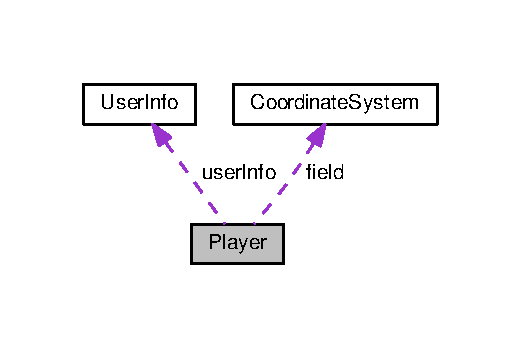
\includegraphics[width=250pt]{classMODEL_1_1Player__coll__graph}
\end{center}
\end{figure}
\subsection*{Public Member Functions}
\begin{DoxyCompactItemize}
\item 
\hyperlink{classMODEL_1_1Player_a244719265958cdd3814a61c97a6e3e98}{Player} ()
\item 
\hyperlink{classMODEL_1_1Player_a6b504bfe315859ffe69a10d3f21829ee}{Player} (const \hyperlink{classUserInfo}{User\+Info} \&\hyperlink{classMODEL_1_1Player_a4ea833995f730252c0bbafea4cf0fdc2}{user\+Info})
\item 
\hyperlink{classMODEL_1_1Player_a85fa038ee81c6c7e1e0a0ecc8304edfd}{Player} (\hyperlink{classMODEL_1_1Player}{Player} const \&)=delete
\item 
\hyperlink{classMODEL_1_1Player}{Player} \& \hyperlink{classMODEL_1_1Player_acf842a8de1ce2116b991b35928c410b9}{operator=} (\hyperlink{classMODEL_1_1Player}{Player} const \&other)=delete
\item 
\hyperlink{classMODEL_1_1Player_aa04e131e23519fa2565393ef59f2291d}{Player} (\hyperlink{classMODEL_1_1Player}{Player} \&\&other)=delete
\item 
\hyperlink{classMODEL_1_1Player}{Player} \& \hyperlink{classMODEL_1_1Player_a96af22c0380c642698eedd0a5112fc33}{operator=} (\hyperlink{classMODEL_1_1Player}{Player} \&\&other)=delete
\item 
void \hyperlink{classMODEL_1_1Player_af9bcbb01780c8dbef6c96c6e75da2442}{set\+User\+Info} (const \hyperlink{classUserInfo}{User\+Info} \&\hyperlink{classMODEL_1_1Player_a4ea833995f730252c0bbafea4cf0fdc2}{user\+Info})
\item 
const \hyperlink{classUserInfo}{User\+Info} \& \hyperlink{classMODEL_1_1Player_a82cbbc06470a73eca6ec268267a9073f}{get\+User\+Info} ()
\item 
\hyperlink{classMODEL_1_1CoordinateSystem}{Coordinate\+System} \& \hyperlink{classMODEL_1_1Player_a705ca7db4cd051354cf500bb7acb266c}{get\+Field} ()
\end{DoxyCompactItemize}
\subsection*{Private Attributes}
\begin{DoxyCompactItemize}
\item 
\hyperlink{classUserInfo}{User\+Info} \hyperlink{classMODEL_1_1Player_a4ea833995f730252c0bbafea4cf0fdc2}{user\+Info}
\item 
\hyperlink{classMODEL_1_1CoordinateSystem}{Coordinate\+System} \hyperlink{classMODEL_1_1Player_a81b1c66a79769f4de04990e7973e1f17}{field}
\end{DoxyCompactItemize}


\subsection{Detailed Description}
A class representing player for model, stores information in \hyperlink{classUserInfo}{User\+Info} object within it. 

\subsection{Constructor \& Destructor Documentation}
\index{M\+O\+D\+E\+L\+::\+Player@{M\+O\+D\+E\+L\+::\+Player}!Player@{Player}}
\index{Player@{Player}!M\+O\+D\+E\+L\+::\+Player@{M\+O\+D\+E\+L\+::\+Player}}
\subsubsection[{\texorpdfstring{Player()}{Player()}}]{\setlength{\rightskip}{0pt plus 5cm}{\bf Player} (
\begin{DoxyParamCaption}
{}
\end{DoxyParamCaption}
)}\hypertarget{classMODEL_1_1Player_a244719265958cdd3814a61c97a6e3e98}{}\label{classMODEL_1_1Player_a244719265958cdd3814a61c97a6e3e98}
\index{M\+O\+D\+E\+L\+::\+Player@{M\+O\+D\+E\+L\+::\+Player}!Player@{Player}}
\index{Player@{Player}!M\+O\+D\+E\+L\+::\+Player@{M\+O\+D\+E\+L\+::\+Player}}
\subsubsection[{\texorpdfstring{Player(const User\+Info \&user\+Info)}{Player(const UserInfo &userInfo)}}]{\setlength{\rightskip}{0pt plus 5cm}{\bf Player} (
\begin{DoxyParamCaption}
\item[{const {\bf User\+Info} \&}]{user\+Info}
\end{DoxyParamCaption}
)}\hypertarget{classMODEL_1_1Player_a6b504bfe315859ffe69a10d3f21829ee}{}\label{classMODEL_1_1Player_a6b504bfe315859ffe69a10d3f21829ee}
\index{M\+O\+D\+E\+L\+::\+Player@{M\+O\+D\+E\+L\+::\+Player}!Player@{Player}}
\index{Player@{Player}!M\+O\+D\+E\+L\+::\+Player@{M\+O\+D\+E\+L\+::\+Player}}
\subsubsection[{\texorpdfstring{Player(\+Player const \&)=delete}{Player(Player const &)=delete}}]{\setlength{\rightskip}{0pt plus 5cm}{\bf Player} (
\begin{DoxyParamCaption}
\item[{{\bf Player} const \&}]{}
\end{DoxyParamCaption}
)\hspace{0.3cm}{\ttfamily [delete]}}\hypertarget{classMODEL_1_1Player_a85fa038ee81c6c7e1e0a0ecc8304edfd}{}\label{classMODEL_1_1Player_a85fa038ee81c6c7e1e0a0ecc8304edfd}
\index{M\+O\+D\+E\+L\+::\+Player@{M\+O\+D\+E\+L\+::\+Player}!Player@{Player}}
\index{Player@{Player}!M\+O\+D\+E\+L\+::\+Player@{M\+O\+D\+E\+L\+::\+Player}}
\subsubsection[{\texorpdfstring{Player(\+Player \&\&other)=delete}{Player(Player &&other)=delete}}]{\setlength{\rightskip}{0pt plus 5cm}{\bf Player} (
\begin{DoxyParamCaption}
\item[{{\bf Player} \&\&}]{other}
\end{DoxyParamCaption}
)\hspace{0.3cm}{\ttfamily [delete]}}\hypertarget{classMODEL_1_1Player_aa04e131e23519fa2565393ef59f2291d}{}\label{classMODEL_1_1Player_aa04e131e23519fa2565393ef59f2291d}


\subsection{Member Function Documentation}
\index{M\+O\+D\+E\+L\+::\+Player@{M\+O\+D\+E\+L\+::\+Player}!get\+Field@{get\+Field}}
\index{get\+Field@{get\+Field}!M\+O\+D\+E\+L\+::\+Player@{M\+O\+D\+E\+L\+::\+Player}}
\subsubsection[{\texorpdfstring{get\+Field()}{getField()}}]{\setlength{\rightskip}{0pt plus 5cm}{\bf M\+O\+D\+E\+L\+::\+Coordinate\+System} \& get\+Field (
\begin{DoxyParamCaption}
{}
\end{DoxyParamCaption}
)}\hypertarget{classMODEL_1_1Player_a705ca7db4cd051354cf500bb7acb266c}{}\label{classMODEL_1_1Player_a705ca7db4cd051354cf500bb7acb266c}
\index{M\+O\+D\+E\+L\+::\+Player@{M\+O\+D\+E\+L\+::\+Player}!get\+User\+Info@{get\+User\+Info}}
\index{get\+User\+Info@{get\+User\+Info}!M\+O\+D\+E\+L\+::\+Player@{M\+O\+D\+E\+L\+::\+Player}}
\subsubsection[{\texorpdfstring{get\+User\+Info()}{getUserInfo()}}]{\setlength{\rightskip}{0pt plus 5cm}const {\bf User\+Info} \& get\+User\+Info (
\begin{DoxyParamCaption}
{}
\end{DoxyParamCaption}
)}\hypertarget{classMODEL_1_1Player_a82cbbc06470a73eca6ec268267a9073f}{}\label{classMODEL_1_1Player_a82cbbc06470a73eca6ec268267a9073f}
\index{M\+O\+D\+E\+L\+::\+Player@{M\+O\+D\+E\+L\+::\+Player}!operator=@{operator=}}
\index{operator=@{operator=}!M\+O\+D\+E\+L\+::\+Player@{M\+O\+D\+E\+L\+::\+Player}}
\subsubsection[{\texorpdfstring{operator=(\+Player const \&other)=delete}{operator=(Player const &other)=delete}}]{\setlength{\rightskip}{0pt plus 5cm}{\bf Player}\& operator= (
\begin{DoxyParamCaption}
\item[{{\bf Player} const \&}]{other}
\end{DoxyParamCaption}
)\hspace{0.3cm}{\ttfamily [delete]}}\hypertarget{classMODEL_1_1Player_acf842a8de1ce2116b991b35928c410b9}{}\label{classMODEL_1_1Player_acf842a8de1ce2116b991b35928c410b9}
\index{M\+O\+D\+E\+L\+::\+Player@{M\+O\+D\+E\+L\+::\+Player}!operator=@{operator=}}
\index{operator=@{operator=}!M\+O\+D\+E\+L\+::\+Player@{M\+O\+D\+E\+L\+::\+Player}}
\subsubsection[{\texorpdfstring{operator=(\+Player \&\&other)=delete}{operator=(Player &&other)=delete}}]{\setlength{\rightskip}{0pt plus 5cm}{\bf Player}\& operator= (
\begin{DoxyParamCaption}
\item[{{\bf Player} \&\&}]{other}
\end{DoxyParamCaption}
)\hspace{0.3cm}{\ttfamily [delete]}}\hypertarget{classMODEL_1_1Player_a96af22c0380c642698eedd0a5112fc33}{}\label{classMODEL_1_1Player_a96af22c0380c642698eedd0a5112fc33}
\index{M\+O\+D\+E\+L\+::\+Player@{M\+O\+D\+E\+L\+::\+Player}!set\+User\+Info@{set\+User\+Info}}
\index{set\+User\+Info@{set\+User\+Info}!M\+O\+D\+E\+L\+::\+Player@{M\+O\+D\+E\+L\+::\+Player}}
\subsubsection[{\texorpdfstring{set\+User\+Info(const User\+Info \&user\+Info)}{setUserInfo(const UserInfo &userInfo)}}]{\setlength{\rightskip}{0pt plus 5cm}void set\+User\+Info (
\begin{DoxyParamCaption}
\item[{const {\bf User\+Info} \&}]{user\+Info}
\end{DoxyParamCaption}
)}\hypertarget{classMODEL_1_1Player_af9bcbb01780c8dbef6c96c6e75da2442}{}\label{classMODEL_1_1Player_af9bcbb01780c8dbef6c96c6e75da2442}


\subsection{Member Data Documentation}
\index{M\+O\+D\+E\+L\+::\+Player@{M\+O\+D\+E\+L\+::\+Player}!field@{field}}
\index{field@{field}!M\+O\+D\+E\+L\+::\+Player@{M\+O\+D\+E\+L\+::\+Player}}
\subsubsection[{\texorpdfstring{field}{field}}]{\setlength{\rightskip}{0pt plus 5cm}{\bf Coordinate\+System} field\hspace{0.3cm}{\ttfamily [private]}}\hypertarget{classMODEL_1_1Player_a81b1c66a79769f4de04990e7973e1f17}{}\label{classMODEL_1_1Player_a81b1c66a79769f4de04990e7973e1f17}
\index{M\+O\+D\+E\+L\+::\+Player@{M\+O\+D\+E\+L\+::\+Player}!user\+Info@{user\+Info}}
\index{user\+Info@{user\+Info}!M\+O\+D\+E\+L\+::\+Player@{M\+O\+D\+E\+L\+::\+Player}}
\subsubsection[{\texorpdfstring{user\+Info}{userInfo}}]{\setlength{\rightskip}{0pt plus 5cm}{\bf User\+Info} user\+Info\hspace{0.3cm}{\ttfamily [private]}}\hypertarget{classMODEL_1_1Player_a4ea833995f730252c0bbafea4cf0fdc2}{}\label{classMODEL_1_1Player_a4ea833995f730252c0bbafea4cf0fdc2}


The documentation for this class was generated from the following files\+:\begin{DoxyCompactItemize}
\item 
model/\hyperlink{model_2player_8h}{player.\+h}\item 
model/\hyperlink{model_2player_8cpp}{player.\+cpp}\end{DoxyCompactItemize}

\hypertarget{classGUI_1_1PlayerForm}{}\section{Player\+Form Class Reference}
\label{classGUI_1_1PlayerForm}\index{Player\+Form@{Player\+Form}}


A simple class that defines graphical interface of the form in which players are able enter the name and age.  




{\ttfamily \#include $<$playerform.\+h$>$}



Inheritance diagram for Player\+Form\+:\nopagebreak
\begin{figure}[H]
\begin{center}
\leavevmode
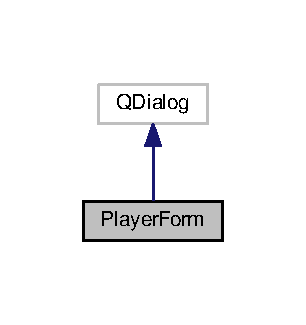
\includegraphics[width=147pt]{classGUI_1_1PlayerForm__inherit__graph}
\end{center}
\end{figure}


Collaboration diagram for Player\+Form\+:\nopagebreak
\begin{figure}[H]
\begin{center}
\leavevmode
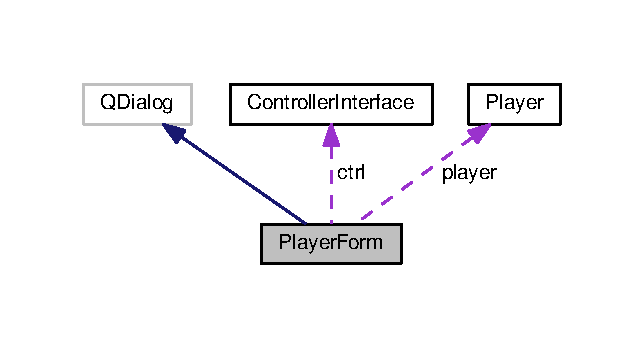
\includegraphics[width=309pt]{classGUI_1_1PlayerForm__coll__graph}
\end{center}
\end{figure}
\subsection*{Public Member Functions}
\begin{DoxyCompactItemize}
\item 
\hyperlink{classGUI_1_1PlayerForm_adb5d9b0acdc6bd505f507533d8769558}{Player\+Form} (\hyperlink{classControllerInterface}{Controller\+Interface} \&\hyperlink{classGUI_1_1PlayerForm_a15e61471831211a4301410bdd802a4a4}{ctrl}, Q\+Widget $\ast$parent=nullptr)
\end{DoxyCompactItemize}
\subsection*{Private Slots}
\begin{DoxyCompactItemize}
\item 
void \hyperlink{classGUI_1_1PlayerForm_aadb9f3b844fb4cf98288cd3c60a3af91}{accept} ()
\end{DoxyCompactItemize}
\subsection*{Private Member Functions}
\begin{DoxyCompactItemize}
\item 
void \hyperlink{classGUI_1_1PlayerForm_a075b75384a607ade082a49f4e05a908d}{create\+Player\+Input\+Fields\+Group} ()
\item 
Q\+Group\+Box $\ast$ \hyperlink{classGUI_1_1PlayerForm_a4964adc00f23438b45887af6a767f09c}{create\+Player\+Connection\+Select\+Group} ()
\item 
bool \hyperlink{classGUI_1_1PlayerForm_ad56866bf1cf64173068b9932ce8e6452}{validate\+User\+Input} ()
\end{DoxyCompactItemize}
\subsection*{Private Attributes}
\begin{DoxyCompactItemize}
\item 
\hyperlink{classControllerInterface}{Controller\+Interface} \& \hyperlink{classGUI_1_1PlayerForm_a15e61471831211a4301410bdd802a4a4}{ctrl}
\item 
\hyperlink{classPlayer}{Player} $\ast$ \hyperlink{classGUI_1_1PlayerForm_a96781128d3743da3d17e0fdd91afba7b}{player}
\item 
Q\+Line\+Edit $\ast$ \hyperlink{classGUI_1_1PlayerForm_a8faa8074b2f9d7f9f4471b1ad61b4c65}{name\+Line}
\item 
Q\+Line\+Edit $\ast$ \hyperlink{classGUI_1_1PlayerForm_a54e5ef4f421180fa1ce8eede3fcfaf53}{age\+Line}
\item 
Q\+Dialog\+Button\+Box $\ast$ \hyperlink{classGUI_1_1PlayerForm_a4d76db11c020d3d895f14dcecf268a95}{button\+Box}
\item 
Q\+Group\+Box $\ast$ \hyperlink{classGUI_1_1PlayerForm_af458ad810116b1284b175480c1a3640e}{horizontal\+Group\+Box}
\item 
Q\+Push\+Button $\ast$ \hyperlink{classGUI_1_1PlayerForm_a2ae9cb3ec8281a3b0b35124cc17c3f3f}{host\+Game\+Btn}
\item 
Q\+Push\+Button $\ast$ \hyperlink{classGUI_1_1PlayerForm_a5890045743cc294ab7d3f08d104818a7}{direct\+Conn\+Btn}
\end{DoxyCompactItemize}


\subsection{Detailed Description}
A simple class that defines graphical interface of the form in which players are able enter the name and age. 

\subsection{Constructor \& Destructor Documentation}
\index{G\+U\+I\+::\+Player\+Form@{G\+U\+I\+::\+Player\+Form}!Player\+Form@{Player\+Form}}
\index{Player\+Form@{Player\+Form}!G\+U\+I\+::\+Player\+Form@{G\+U\+I\+::\+Player\+Form}}
\subsubsection[{\texorpdfstring{Player\+Form(\+Controller\+Interface \&ctrl, Q\+Widget $\ast$parent=nullptr)}{PlayerForm(ControllerInterface &ctrl, QWidget *parent=nullptr)}}]{\setlength{\rightskip}{0pt plus 5cm}{\bf Player\+Form} (
\begin{DoxyParamCaption}
\item[{{\bf Controller\+Interface} \&}]{ctrl, }
\item[{Q\+Widget $\ast$}]{parent = {\ttfamily nullptr}}
\end{DoxyParamCaption}
)}\hypertarget{classGUI_1_1PlayerForm_adb5d9b0acdc6bd505f507533d8769558}{}\label{classGUI_1_1PlayerForm_adb5d9b0acdc6bd505f507533d8769558}


\subsection{Member Function Documentation}
\index{G\+U\+I\+::\+Player\+Form@{G\+U\+I\+::\+Player\+Form}!accept@{accept}}
\index{accept@{accept}!G\+U\+I\+::\+Player\+Form@{G\+U\+I\+::\+Player\+Form}}
\subsubsection[{\texorpdfstring{accept}{accept}}]{\setlength{\rightskip}{0pt plus 5cm}void accept (
\begin{DoxyParamCaption}
{}
\end{DoxyParamCaption}
)\hspace{0.3cm}{\ttfamily [private]}, {\ttfamily [slot]}}\hypertarget{classGUI_1_1PlayerForm_aadb9f3b844fb4cf98288cd3c60a3af91}{}\label{classGUI_1_1PlayerForm_aadb9f3b844fb4cf98288cd3c60a3af91}
\index{G\+U\+I\+::\+Player\+Form@{G\+U\+I\+::\+Player\+Form}!create\+Player\+Connection\+Select\+Group@{create\+Player\+Connection\+Select\+Group}}
\index{create\+Player\+Connection\+Select\+Group@{create\+Player\+Connection\+Select\+Group}!G\+U\+I\+::\+Player\+Form@{G\+U\+I\+::\+Player\+Form}}
\subsubsection[{\texorpdfstring{create\+Player\+Connection\+Select\+Group()}{createPlayerConnectionSelectGroup()}}]{\setlength{\rightskip}{0pt plus 5cm}Q\+Group\+Box $\ast$ create\+Player\+Connection\+Select\+Group (
\begin{DoxyParamCaption}
{}
\end{DoxyParamCaption}
)\hspace{0.3cm}{\ttfamily [private]}}\hypertarget{classGUI_1_1PlayerForm_a4964adc00f23438b45887af6a767f09c}{}\label{classGUI_1_1PlayerForm_a4964adc00f23438b45887af6a767f09c}
\index{G\+U\+I\+::\+Player\+Form@{G\+U\+I\+::\+Player\+Form}!create\+Player\+Input\+Fields\+Group@{create\+Player\+Input\+Fields\+Group}}
\index{create\+Player\+Input\+Fields\+Group@{create\+Player\+Input\+Fields\+Group}!G\+U\+I\+::\+Player\+Form@{G\+U\+I\+::\+Player\+Form}}
\subsubsection[{\texorpdfstring{create\+Player\+Input\+Fields\+Group()}{createPlayerInputFieldsGroup()}}]{\setlength{\rightskip}{0pt plus 5cm}void create\+Player\+Input\+Fields\+Group (
\begin{DoxyParamCaption}
{}
\end{DoxyParamCaption}
)\hspace{0.3cm}{\ttfamily [private]}}\hypertarget{classGUI_1_1PlayerForm_a075b75384a607ade082a49f4e05a908d}{}\label{classGUI_1_1PlayerForm_a075b75384a607ade082a49f4e05a908d}
\index{G\+U\+I\+::\+Player\+Form@{G\+U\+I\+::\+Player\+Form}!validate\+User\+Input@{validate\+User\+Input}}
\index{validate\+User\+Input@{validate\+User\+Input}!G\+U\+I\+::\+Player\+Form@{G\+U\+I\+::\+Player\+Form}}
\subsubsection[{\texorpdfstring{validate\+User\+Input()}{validateUserInput()}}]{\setlength{\rightskip}{0pt plus 5cm}bool validate\+User\+Input (
\begin{DoxyParamCaption}
{}
\end{DoxyParamCaption}
)\hspace{0.3cm}{\ttfamily [private]}}\hypertarget{classGUI_1_1PlayerForm_ad56866bf1cf64173068b9932ce8e6452}{}\label{classGUI_1_1PlayerForm_ad56866bf1cf64173068b9932ce8e6452}
\begin{DoxyReturn}{Returns}
true if name is not empty 
\end{DoxyReturn}


\subsection{Member Data Documentation}
\index{G\+U\+I\+::\+Player\+Form@{G\+U\+I\+::\+Player\+Form}!age\+Line@{age\+Line}}
\index{age\+Line@{age\+Line}!G\+U\+I\+::\+Player\+Form@{G\+U\+I\+::\+Player\+Form}}
\subsubsection[{\texorpdfstring{age\+Line}{ageLine}}]{\setlength{\rightskip}{0pt plus 5cm}Q\+Line\+Edit$\ast$ age\+Line\hspace{0.3cm}{\ttfamily [private]}}\hypertarget{classGUI_1_1PlayerForm_a54e5ef4f421180fa1ce8eede3fcfaf53}{}\label{classGUI_1_1PlayerForm_a54e5ef4f421180fa1ce8eede3fcfaf53}
\index{G\+U\+I\+::\+Player\+Form@{G\+U\+I\+::\+Player\+Form}!button\+Box@{button\+Box}}
\index{button\+Box@{button\+Box}!G\+U\+I\+::\+Player\+Form@{G\+U\+I\+::\+Player\+Form}}
\subsubsection[{\texorpdfstring{button\+Box}{buttonBox}}]{\setlength{\rightskip}{0pt plus 5cm}Q\+Dialog\+Button\+Box$\ast$ button\+Box\hspace{0.3cm}{\ttfamily [private]}}\hypertarget{classGUI_1_1PlayerForm_a4d76db11c020d3d895f14dcecf268a95}{}\label{classGUI_1_1PlayerForm_a4d76db11c020d3d895f14dcecf268a95}
\index{G\+U\+I\+::\+Player\+Form@{G\+U\+I\+::\+Player\+Form}!ctrl@{ctrl}}
\index{ctrl@{ctrl}!G\+U\+I\+::\+Player\+Form@{G\+U\+I\+::\+Player\+Form}}
\subsubsection[{\texorpdfstring{ctrl}{ctrl}}]{\setlength{\rightskip}{0pt plus 5cm}{\bf Controller\+Interface}\& ctrl\hspace{0.3cm}{\ttfamily [private]}}\hypertarget{classGUI_1_1PlayerForm_a15e61471831211a4301410bdd802a4a4}{}\label{classGUI_1_1PlayerForm_a15e61471831211a4301410bdd802a4a4}
\index{G\+U\+I\+::\+Player\+Form@{G\+U\+I\+::\+Player\+Form}!direct\+Conn\+Btn@{direct\+Conn\+Btn}}
\index{direct\+Conn\+Btn@{direct\+Conn\+Btn}!G\+U\+I\+::\+Player\+Form@{G\+U\+I\+::\+Player\+Form}}
\subsubsection[{\texorpdfstring{direct\+Conn\+Btn}{directConnBtn}}]{\setlength{\rightskip}{0pt plus 5cm}Q\+Push\+Button$\ast$ direct\+Conn\+Btn\hspace{0.3cm}{\ttfamily [private]}}\hypertarget{classGUI_1_1PlayerForm_a5890045743cc294ab7d3f08d104818a7}{}\label{classGUI_1_1PlayerForm_a5890045743cc294ab7d3f08d104818a7}
\index{G\+U\+I\+::\+Player\+Form@{G\+U\+I\+::\+Player\+Form}!horizontal\+Group\+Box@{horizontal\+Group\+Box}}
\index{horizontal\+Group\+Box@{horizontal\+Group\+Box}!G\+U\+I\+::\+Player\+Form@{G\+U\+I\+::\+Player\+Form}}
\subsubsection[{\texorpdfstring{horizontal\+Group\+Box}{horizontalGroupBox}}]{\setlength{\rightskip}{0pt plus 5cm}Q\+Group\+Box$\ast$ horizontal\+Group\+Box\hspace{0.3cm}{\ttfamily [private]}}\hypertarget{classGUI_1_1PlayerForm_af458ad810116b1284b175480c1a3640e}{}\label{classGUI_1_1PlayerForm_af458ad810116b1284b175480c1a3640e}
\index{G\+U\+I\+::\+Player\+Form@{G\+U\+I\+::\+Player\+Form}!host\+Game\+Btn@{host\+Game\+Btn}}
\index{host\+Game\+Btn@{host\+Game\+Btn}!G\+U\+I\+::\+Player\+Form@{G\+U\+I\+::\+Player\+Form}}
\subsubsection[{\texorpdfstring{host\+Game\+Btn}{hostGameBtn}}]{\setlength{\rightskip}{0pt plus 5cm}Q\+Push\+Button$\ast$ host\+Game\+Btn\hspace{0.3cm}{\ttfamily [private]}}\hypertarget{classGUI_1_1PlayerForm_a2ae9cb3ec8281a3b0b35124cc17c3f3f}{}\label{classGUI_1_1PlayerForm_a2ae9cb3ec8281a3b0b35124cc17c3f3f}
\index{G\+U\+I\+::\+Player\+Form@{G\+U\+I\+::\+Player\+Form}!name\+Line@{name\+Line}}
\index{name\+Line@{name\+Line}!G\+U\+I\+::\+Player\+Form@{G\+U\+I\+::\+Player\+Form}}
\subsubsection[{\texorpdfstring{name\+Line}{nameLine}}]{\setlength{\rightskip}{0pt plus 5cm}Q\+Line\+Edit$\ast$ name\+Line\hspace{0.3cm}{\ttfamily [private]}}\hypertarget{classGUI_1_1PlayerForm_a8faa8074b2f9d7f9f4471b1ad61b4c65}{}\label{classGUI_1_1PlayerForm_a8faa8074b2f9d7f9f4471b1ad61b4c65}
\index{G\+U\+I\+::\+Player\+Form@{G\+U\+I\+::\+Player\+Form}!player@{player}}
\index{player@{player}!G\+U\+I\+::\+Player\+Form@{G\+U\+I\+::\+Player\+Form}}
\subsubsection[{\texorpdfstring{player}{player}}]{\setlength{\rightskip}{0pt plus 5cm}{\bf Player}$\ast$ player\hspace{0.3cm}{\ttfamily [private]}}\hypertarget{classGUI_1_1PlayerForm_a96781128d3743da3d17e0fdd91afba7b}{}\label{classGUI_1_1PlayerForm_a96781128d3743da3d17e0fdd91afba7b}


The documentation for this class was generated from the following files\+:\begin{DoxyCompactItemize}
\item 
gui/\hyperlink{playerform_8h}{playerform.\+h}\item 
gui/\hyperlink{playerform_8cpp}{playerform.\+cpp}\end{DoxyCompactItemize}

\hypertarget{classMODEL_1_1Point}{}\section{Point Class Reference}
\label{classMODEL_1_1Point}\index{Point@{Point}}


A simple class representing point.  




{\ttfamily \#include $<$point.\+h$>$}

\subsection*{Public Member Functions}
\begin{DoxyCompactItemize}
\item 
\hyperlink{classMODEL_1_1Point_a8eb76552ab4daf01a92da58843a0253b}{Point} (double \hyperlink{classMODEL_1_1Point_af88b946fb90d5f08b5fb740c70e98c10}{x}, double \hyperlink{classMODEL_1_1Point_ab927965981178aa1fba979a37168db2a}{y})
\item 
double \hyperlink{classMODEL_1_1Point_a2b69e4312b7814c6efce42f851893409}{getX} ()
\item 
double \hyperlink{classMODEL_1_1Point_a15f19cf52955c8c3406831b288681358}{getY} ()
\end{DoxyCompactItemize}
\subsection*{Private Attributes}
\begin{DoxyCompactItemize}
\item 
double \hyperlink{classMODEL_1_1Point_af88b946fb90d5f08b5fb740c70e98c10}{x}
\item 
double \hyperlink{classMODEL_1_1Point_ab927965981178aa1fba979a37168db2a}{y}
\end{DoxyCompactItemize}


\subsection{Detailed Description}
A simple class representing point. 

\subsection{Constructor \& Destructor Documentation}
\index{M\+O\+D\+E\+L\+::\+Point@{M\+O\+D\+E\+L\+::\+Point}!Point@{Point}}
\index{Point@{Point}!M\+O\+D\+E\+L\+::\+Point@{M\+O\+D\+E\+L\+::\+Point}}
\subsubsection[{\texorpdfstring{Point(double x, double y)}{Point(double x, double y)}}]{\setlength{\rightskip}{0pt plus 5cm}{\bf Point} (
\begin{DoxyParamCaption}
\item[{double}]{x, }
\item[{double}]{y}
\end{DoxyParamCaption}
)\hspace{0.3cm}{\ttfamily [explicit]}}\hypertarget{classMODEL_1_1Point_a8eb76552ab4daf01a92da58843a0253b}{}\label{classMODEL_1_1Point_a8eb76552ab4daf01a92da58843a0253b}


\subsection{Member Function Documentation}
\index{M\+O\+D\+E\+L\+::\+Point@{M\+O\+D\+E\+L\+::\+Point}!getX@{getX}}
\index{getX@{getX}!M\+O\+D\+E\+L\+::\+Point@{M\+O\+D\+E\+L\+::\+Point}}
\subsubsection[{\texorpdfstring{get\+X()}{getX()}}]{\setlength{\rightskip}{0pt plus 5cm}double getX (
\begin{DoxyParamCaption}
{}
\end{DoxyParamCaption}
)}\hypertarget{classMODEL_1_1Point_a2b69e4312b7814c6efce42f851893409}{}\label{classMODEL_1_1Point_a2b69e4312b7814c6efce42f851893409}
\index{M\+O\+D\+E\+L\+::\+Point@{M\+O\+D\+E\+L\+::\+Point}!getY@{getY}}
\index{getY@{getY}!M\+O\+D\+E\+L\+::\+Point@{M\+O\+D\+E\+L\+::\+Point}}
\subsubsection[{\texorpdfstring{get\+Y()}{getY()}}]{\setlength{\rightskip}{0pt plus 5cm}double getY (
\begin{DoxyParamCaption}
{}
\end{DoxyParamCaption}
)}\hypertarget{classMODEL_1_1Point_a15f19cf52955c8c3406831b288681358}{}\label{classMODEL_1_1Point_a15f19cf52955c8c3406831b288681358}


\subsection{Member Data Documentation}
\index{M\+O\+D\+E\+L\+::\+Point@{M\+O\+D\+E\+L\+::\+Point}!x@{x}}
\index{x@{x}!M\+O\+D\+E\+L\+::\+Point@{M\+O\+D\+E\+L\+::\+Point}}
\subsubsection[{\texorpdfstring{x}{x}}]{\setlength{\rightskip}{0pt plus 5cm}double x\hspace{0.3cm}{\ttfamily [private]}}\hypertarget{classMODEL_1_1Point_af88b946fb90d5f08b5fb740c70e98c10}{}\label{classMODEL_1_1Point_af88b946fb90d5f08b5fb740c70e98c10}
\index{M\+O\+D\+E\+L\+::\+Point@{M\+O\+D\+E\+L\+::\+Point}!y@{y}}
\index{y@{y}!M\+O\+D\+E\+L\+::\+Point@{M\+O\+D\+E\+L\+::\+Point}}
\subsubsection[{\texorpdfstring{y}{y}}]{\setlength{\rightskip}{0pt plus 5cm}double y\hspace{0.3cm}{\ttfamily [private]}}\hypertarget{classMODEL_1_1Point_ab927965981178aa1fba979a37168db2a}{}\label{classMODEL_1_1Point_ab927965981178aa1fba979a37168db2a}


The documentation for this class was generated from the following files\+:\begin{DoxyCompactItemize}
\item 
model/\hyperlink{point_8h}{point.\+h}\item 
model/\hyperlink{point_8cpp}{point.\+cpp}\end{DoxyCompactItemize}

\hypertarget{classSetShipsForm}{}\section{Set\+Ships\+Form Class Reference}
\label{classSetShipsForm}\index{Set\+Ships\+Form@{Set\+Ships\+Form}}


A simple class that defines graphical interface of the form in which players are able to set ships.  




{\ttfamily \#include $<$setshipsform.\+h$>$}



Inheritance diagram for Set\+Ships\+Form\+:\nopagebreak
\begin{figure}[H]
\begin{center}
\leavevmode
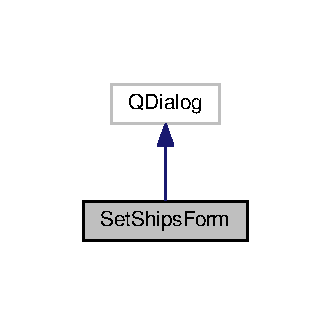
\includegraphics[width=159pt]{classSetShipsForm__inherit__graph}
\end{center}
\end{figure}


Collaboration diagram for Set\+Ships\+Form\+:\nopagebreak
\begin{figure}[H]
\begin{center}
\leavevmode
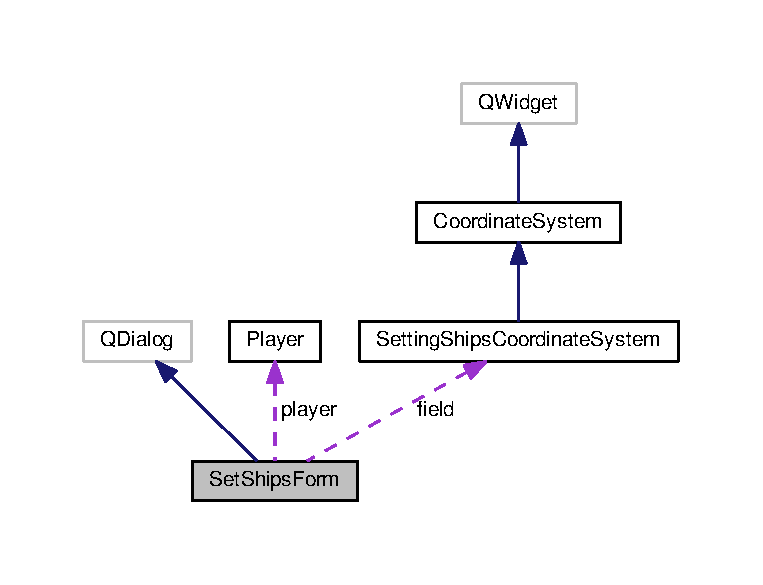
\includegraphics[width=350pt]{classSetShipsForm__coll__graph}
\end{center}
\end{figure}
\subsection*{Public Member Functions}
\begin{DoxyCompactItemize}
\item 
\hyperlink{classSetShipsForm_a5d8d0b3ae99ed33ab7f86da618853892}{Set\+Ships\+Form} (\hyperlink{classPlayer}{Player} $\ast$\hyperlink{classSetShipsForm_a96781128d3743da3d17e0fdd91afba7b}{player})
\end{DoxyCompactItemize}
\subsection*{Private Slots}
\begin{DoxyCompactItemize}
\item 
void \hyperlink{classSetShipsForm_a9a5bd99aaa8c0771d6d667c0b4236b22}{delete\+Ships} ()
\end{DoxyCompactItemize}
\subsection*{Private Member Functions}
\begin{DoxyCompactItemize}
\item 
void \hyperlink{classSetShipsForm_a84e8aba32191c603553509d5248ee4b5}{create\+Menu} ()
\item 
void \hyperlink{classSetShipsForm_a497d3ad24737683529f9f87b98fd3b67}{create\+Player\+Information\+Group\+Box} ()
\item 
void \hyperlink{classSetShipsForm_a94aecc37ca7712b0e59f69d353bcc84e}{create\+Coordinate\+System\+Group\+Box} ()
\item 
void \hyperlink{classSetShipsForm_a3f341efc111e193ae9b69e107f994e1e}{create\+Form\+Group\+Box} ()
\item 
void \hyperlink{classSetShipsForm_aadb9f3b844fb4cf98288cd3c60a3af91}{accept} ()
\end{DoxyCompactItemize}
\subsection*{Private Attributes}
\begin{DoxyCompactItemize}
\item 
Q\+Menu\+Bar $\ast$ \hyperlink{classSetShipsForm_af1e1fab084abbaa2eb09807c6f403a9b}{menu\+Bar}
\item 
Q\+Menu $\ast$ \hyperlink{classSetShipsForm_ac7360174a0bfa93d26e5c7869c1ef093}{game\+Menu}
\item 
Q\+Action $\ast$ \hyperlink{classSetShipsForm_a95088aac220cb7eb4159ab75d86cb81d}{exit\+Action}
\item 
Q\+Action $\ast$ \hyperlink{classSetShipsForm_ab1f248f26fd94e38178e5e5d1bd5b36c}{delete\+Ships\+Action}
\item 
Q\+Group\+Box $\ast$ \hyperlink{classSetShipsForm_ad382b647f03157d361b01d38047aa9c2}{player\+Information\+Group\+Box}
\item 
Q\+Group\+Box $\ast$ \hyperlink{classSetShipsForm_aa71dd8262fdba4230d1072a845520698}{coordinate\+System\+Group\+Box}
\item 
Q\+Dialog\+Button\+Box $\ast$ \hyperlink{classSetShipsForm_a4d76db11c020d3d895f14dcecf268a95}{button\+Box}
\item 
\hyperlink{classGUI_1_1SettingShipsCoordinateSystem}{G\+U\+I\+::\+Setting\+Ships\+Coordinate\+System} $\ast$ \hyperlink{classSetShipsForm_a09111d953f1f3811661c4947c155dbfb}{field}
\item 
\hyperlink{classPlayer}{Player} $\ast$ \hyperlink{classSetShipsForm_a96781128d3743da3d17e0fdd91afba7b}{player}
\item 
Q\+Label $\ast$ \hyperlink{classSetShipsForm_a234f9726dc5a645e96bdc469aeda8f18}{name\+Label}
\item 
const Q\+Size \hyperlink{classSetShipsForm_a28b453b66a8e010eaaab755d702f299d}{size}
\end{DoxyCompactItemize}


\subsection{Detailed Description}
A simple class that defines graphical interface of the form in which players are able to set ships. 

\subsection{Constructor \& Destructor Documentation}
\index{Set\+Ships\+Form@{Set\+Ships\+Form}!Set\+Ships\+Form@{Set\+Ships\+Form}}
\index{Set\+Ships\+Form@{Set\+Ships\+Form}!Set\+Ships\+Form@{Set\+Ships\+Form}}
\subsubsection[{\texorpdfstring{Set\+Ships\+Form(\+Player $\ast$player)}{SetShipsForm(Player *player)}}]{\setlength{\rightskip}{0pt plus 5cm}{\bf Set\+Ships\+Form} (
\begin{DoxyParamCaption}
\item[{{\bf Player} $\ast$}]{player}
\end{DoxyParamCaption}
)}\hypertarget{classSetShipsForm_a5d8d0b3ae99ed33ab7f86da618853892}{}\label{classSetShipsForm_a5d8d0b3ae99ed33ab7f86da618853892}


\subsection{Member Function Documentation}
\index{Set\+Ships\+Form@{Set\+Ships\+Form}!accept@{accept}}
\index{accept@{accept}!Set\+Ships\+Form@{Set\+Ships\+Form}}
\subsubsection[{\texorpdfstring{accept()}{accept()}}]{\setlength{\rightskip}{0pt plus 5cm}void accept (
\begin{DoxyParamCaption}
{}
\end{DoxyParamCaption}
)\hspace{0.3cm}{\ttfamily [private]}}\hypertarget{classSetShipsForm_aadb9f3b844fb4cf98288cd3c60a3af91}{}\label{classSetShipsForm_aadb9f3b844fb4cf98288cd3c60a3af91}
\index{Set\+Ships\+Form@{Set\+Ships\+Form}!create\+Coordinate\+System\+Group\+Box@{create\+Coordinate\+System\+Group\+Box}}
\index{create\+Coordinate\+System\+Group\+Box@{create\+Coordinate\+System\+Group\+Box}!Set\+Ships\+Form@{Set\+Ships\+Form}}
\subsubsection[{\texorpdfstring{create\+Coordinate\+System\+Group\+Box()}{createCoordinateSystemGroupBox()}}]{\setlength{\rightskip}{0pt plus 5cm}void create\+Coordinate\+System\+Group\+Box (
\begin{DoxyParamCaption}
{}
\end{DoxyParamCaption}
)\hspace{0.3cm}{\ttfamily [private]}}\hypertarget{classSetShipsForm_a94aecc37ca7712b0e59f69d353bcc84e}{}\label{classSetShipsForm_a94aecc37ca7712b0e59f69d353bcc84e}
\index{Set\+Ships\+Form@{Set\+Ships\+Form}!create\+Form\+Group\+Box@{create\+Form\+Group\+Box}}
\index{create\+Form\+Group\+Box@{create\+Form\+Group\+Box}!Set\+Ships\+Form@{Set\+Ships\+Form}}
\subsubsection[{\texorpdfstring{create\+Form\+Group\+Box()}{createFormGroupBox()}}]{\setlength{\rightskip}{0pt plus 5cm}void create\+Form\+Group\+Box (
\begin{DoxyParamCaption}
{}
\end{DoxyParamCaption}
)\hspace{0.3cm}{\ttfamily [private]}}\hypertarget{classSetShipsForm_a3f341efc111e193ae9b69e107f994e1e}{}\label{classSetShipsForm_a3f341efc111e193ae9b69e107f994e1e}
\index{Set\+Ships\+Form@{Set\+Ships\+Form}!create\+Menu@{create\+Menu}}
\index{create\+Menu@{create\+Menu}!Set\+Ships\+Form@{Set\+Ships\+Form}}
\subsubsection[{\texorpdfstring{create\+Menu()}{createMenu()}}]{\setlength{\rightskip}{0pt plus 5cm}void create\+Menu (
\begin{DoxyParamCaption}
{}
\end{DoxyParamCaption}
)\hspace{0.3cm}{\ttfamily [private]}}\hypertarget{classSetShipsForm_a84e8aba32191c603553509d5248ee4b5}{}\label{classSetShipsForm_a84e8aba32191c603553509d5248ee4b5}
\index{Set\+Ships\+Form@{Set\+Ships\+Form}!create\+Player\+Information\+Group\+Box@{create\+Player\+Information\+Group\+Box}}
\index{create\+Player\+Information\+Group\+Box@{create\+Player\+Information\+Group\+Box}!Set\+Ships\+Form@{Set\+Ships\+Form}}
\subsubsection[{\texorpdfstring{create\+Player\+Information\+Group\+Box()}{createPlayerInformationGroupBox()}}]{\setlength{\rightskip}{0pt plus 5cm}void create\+Player\+Information\+Group\+Box (
\begin{DoxyParamCaption}
{}
\end{DoxyParamCaption}
)\hspace{0.3cm}{\ttfamily [private]}}\hypertarget{classSetShipsForm_a497d3ad24737683529f9f87b98fd3b67}{}\label{classSetShipsForm_a497d3ad24737683529f9f87b98fd3b67}
\index{Set\+Ships\+Form@{Set\+Ships\+Form}!delete\+Ships@{delete\+Ships}}
\index{delete\+Ships@{delete\+Ships}!Set\+Ships\+Form@{Set\+Ships\+Form}}
\subsubsection[{\texorpdfstring{delete\+Ships}{deleteShips}}]{\setlength{\rightskip}{0pt plus 5cm}void delete\+Ships (
\begin{DoxyParamCaption}
{}
\end{DoxyParamCaption}
)\hspace{0.3cm}{\ttfamily [private]}, {\ttfamily [slot]}}\hypertarget{classSetShipsForm_a9a5bd99aaa8c0771d6d667c0b4236b22}{}\label{classSetShipsForm_a9a5bd99aaa8c0771d6d667c0b4236b22}


\subsection{Member Data Documentation}
\index{Set\+Ships\+Form@{Set\+Ships\+Form}!button\+Box@{button\+Box}}
\index{button\+Box@{button\+Box}!Set\+Ships\+Form@{Set\+Ships\+Form}}
\subsubsection[{\texorpdfstring{button\+Box}{buttonBox}}]{\setlength{\rightskip}{0pt plus 5cm}Q\+Dialog\+Button\+Box$\ast$ button\+Box\hspace{0.3cm}{\ttfamily [private]}}\hypertarget{classSetShipsForm_a4d76db11c020d3d895f14dcecf268a95}{}\label{classSetShipsForm_a4d76db11c020d3d895f14dcecf268a95}
\index{Set\+Ships\+Form@{Set\+Ships\+Form}!coordinate\+System\+Group\+Box@{coordinate\+System\+Group\+Box}}
\index{coordinate\+System\+Group\+Box@{coordinate\+System\+Group\+Box}!Set\+Ships\+Form@{Set\+Ships\+Form}}
\subsubsection[{\texorpdfstring{coordinate\+System\+Group\+Box}{coordinateSystemGroupBox}}]{\setlength{\rightskip}{0pt plus 5cm}Q\+Group\+Box$\ast$ coordinate\+System\+Group\+Box\hspace{0.3cm}{\ttfamily [private]}}\hypertarget{classSetShipsForm_aa71dd8262fdba4230d1072a845520698}{}\label{classSetShipsForm_aa71dd8262fdba4230d1072a845520698}
\index{Set\+Ships\+Form@{Set\+Ships\+Form}!delete\+Ships\+Action@{delete\+Ships\+Action}}
\index{delete\+Ships\+Action@{delete\+Ships\+Action}!Set\+Ships\+Form@{Set\+Ships\+Form}}
\subsubsection[{\texorpdfstring{delete\+Ships\+Action}{deleteShipsAction}}]{\setlength{\rightskip}{0pt plus 5cm}Q\+Action$\ast$ delete\+Ships\+Action\hspace{0.3cm}{\ttfamily [private]}}\hypertarget{classSetShipsForm_ab1f248f26fd94e38178e5e5d1bd5b36c}{}\label{classSetShipsForm_ab1f248f26fd94e38178e5e5d1bd5b36c}
\index{Set\+Ships\+Form@{Set\+Ships\+Form}!exit\+Action@{exit\+Action}}
\index{exit\+Action@{exit\+Action}!Set\+Ships\+Form@{Set\+Ships\+Form}}
\subsubsection[{\texorpdfstring{exit\+Action}{exitAction}}]{\setlength{\rightskip}{0pt plus 5cm}Q\+Action$\ast$ exit\+Action\hspace{0.3cm}{\ttfamily [private]}}\hypertarget{classSetShipsForm_a95088aac220cb7eb4159ab75d86cb81d}{}\label{classSetShipsForm_a95088aac220cb7eb4159ab75d86cb81d}
\index{Set\+Ships\+Form@{Set\+Ships\+Form}!field@{field}}
\index{field@{field}!Set\+Ships\+Form@{Set\+Ships\+Form}}
\subsubsection[{\texorpdfstring{field}{field}}]{\setlength{\rightskip}{0pt plus 5cm}{\bf G\+U\+I\+::\+Setting\+Ships\+Coordinate\+System}$\ast$ field\hspace{0.3cm}{\ttfamily [private]}}\hypertarget{classSetShipsForm_a09111d953f1f3811661c4947c155dbfb}{}\label{classSetShipsForm_a09111d953f1f3811661c4947c155dbfb}
\index{Set\+Ships\+Form@{Set\+Ships\+Form}!game\+Menu@{game\+Menu}}
\index{game\+Menu@{game\+Menu}!Set\+Ships\+Form@{Set\+Ships\+Form}}
\subsubsection[{\texorpdfstring{game\+Menu}{gameMenu}}]{\setlength{\rightskip}{0pt plus 5cm}Q\+Menu$\ast$ game\+Menu\hspace{0.3cm}{\ttfamily [private]}}\hypertarget{classSetShipsForm_ac7360174a0bfa93d26e5c7869c1ef093}{}\label{classSetShipsForm_ac7360174a0bfa93d26e5c7869c1ef093}
\index{Set\+Ships\+Form@{Set\+Ships\+Form}!menu\+Bar@{menu\+Bar}}
\index{menu\+Bar@{menu\+Bar}!Set\+Ships\+Form@{Set\+Ships\+Form}}
\subsubsection[{\texorpdfstring{menu\+Bar}{menuBar}}]{\setlength{\rightskip}{0pt plus 5cm}Q\+Menu\+Bar$\ast$ menu\+Bar\hspace{0.3cm}{\ttfamily [private]}}\hypertarget{classSetShipsForm_af1e1fab084abbaa2eb09807c6f403a9b}{}\label{classSetShipsForm_af1e1fab084abbaa2eb09807c6f403a9b}
\index{Set\+Ships\+Form@{Set\+Ships\+Form}!name\+Label@{name\+Label}}
\index{name\+Label@{name\+Label}!Set\+Ships\+Form@{Set\+Ships\+Form}}
\subsubsection[{\texorpdfstring{name\+Label}{nameLabel}}]{\setlength{\rightskip}{0pt plus 5cm}Q\+Label$\ast$ name\+Label\hspace{0.3cm}{\ttfamily [private]}}\hypertarget{classSetShipsForm_a234f9726dc5a645e96bdc469aeda8f18}{}\label{classSetShipsForm_a234f9726dc5a645e96bdc469aeda8f18}
\index{Set\+Ships\+Form@{Set\+Ships\+Form}!player@{player}}
\index{player@{player}!Set\+Ships\+Form@{Set\+Ships\+Form}}
\subsubsection[{\texorpdfstring{player}{player}}]{\setlength{\rightskip}{0pt plus 5cm}{\bf Player}$\ast$ player\hspace{0.3cm}{\ttfamily [private]}}\hypertarget{classSetShipsForm_a96781128d3743da3d17e0fdd91afba7b}{}\label{classSetShipsForm_a96781128d3743da3d17e0fdd91afba7b}
\index{Set\+Ships\+Form@{Set\+Ships\+Form}!player\+Information\+Group\+Box@{player\+Information\+Group\+Box}}
\index{player\+Information\+Group\+Box@{player\+Information\+Group\+Box}!Set\+Ships\+Form@{Set\+Ships\+Form}}
\subsubsection[{\texorpdfstring{player\+Information\+Group\+Box}{playerInformationGroupBox}}]{\setlength{\rightskip}{0pt plus 5cm}Q\+Group\+Box$\ast$ player\+Information\+Group\+Box\hspace{0.3cm}{\ttfamily [private]}}\hypertarget{classSetShipsForm_ad382b647f03157d361b01d38047aa9c2}{}\label{classSetShipsForm_ad382b647f03157d361b01d38047aa9c2}
\index{Set\+Ships\+Form@{Set\+Ships\+Form}!size@{size}}
\index{size@{size}!Set\+Ships\+Form@{Set\+Ships\+Form}}
\subsubsection[{\texorpdfstring{size}{size}}]{\setlength{\rightskip}{0pt plus 5cm}const Q\+Size size\hspace{0.3cm}{\ttfamily [private]}}\hypertarget{classSetShipsForm_a28b453b66a8e010eaaab755d702f299d}{}\label{classSetShipsForm_a28b453b66a8e010eaaab755d702f299d}


The documentation for this class was generated from the following files\+:\begin{DoxyCompactItemize}
\item 
gui/\hyperlink{setshipsform_8h}{setshipsform.\+h}\item 
gui/\hyperlink{setshipsform_8cpp}{setshipsform.\+cpp}\end{DoxyCompactItemize}

\hypertarget{classGUI_1_1SettingShipsCoordinateSystem}{}\section{Setting\+Ships\+Coordinate\+System Class Reference}
\label{classGUI_1_1SettingShipsCoordinateSystem}\index{Setting\+Ships\+Coordinate\+System@{Setting\+Ships\+Coordinate\+System}}


A simple class that inherits from \hyperlink{classGUI_1_1CoordinateSystem}{Coordinate\+System} and implements mouse events for setting ships.  




{\ttfamily \#include $<$settingshipscoordinatesystem.\+h$>$}



Inheritance diagram for Setting\+Ships\+Coordinate\+System\+:\nopagebreak
\begin{figure}[H]
\begin{center}
\leavevmode
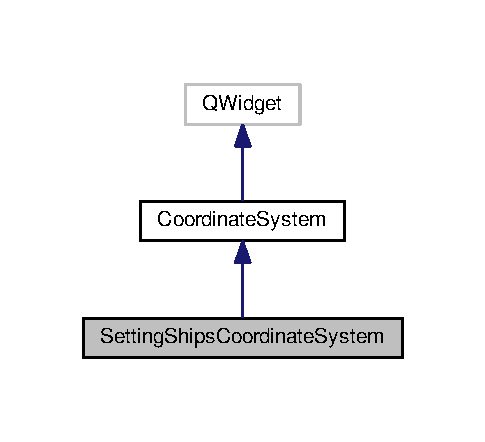
\includegraphics[width=233pt]{classGUI_1_1SettingShipsCoordinateSystem__inherit__graph}
\end{center}
\end{figure}


Collaboration diagram for Setting\+Ships\+Coordinate\+System\+:\nopagebreak
\begin{figure}[H]
\begin{center}
\leavevmode
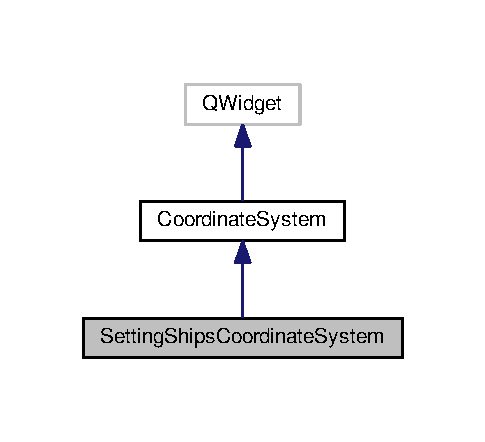
\includegraphics[width=233pt]{classGUI_1_1SettingShipsCoordinateSystem__coll__graph}
\end{center}
\end{figure}
\subsection*{Public Member Functions}
\begin{DoxyCompactItemize}
\item 
\hyperlink{classGUI_1_1SettingShipsCoordinateSystem_a1043bd36a10f81e768fd9378d870d639}{$\sim$\+Setting\+Ships\+Coordinate\+System} ()
\item 
void \hyperlink{classGUI_1_1SettingShipsCoordinateSystem_abcb8de61d1e6998fbc06813adfebde57}{fill\+Points\+List} ()
\item 
Q\+Point \hyperlink{classGUI_1_1SettingShipsCoordinateSystem_a98993f7ed1af6efcbdc1e75414ccd7c8}{get\+Next\+Point\+From\+Vector} (int, int, std\+::vector$<$ Q\+Point $>$ \&)
\item 
void \hyperlink{classGUI_1_1SettingShipsCoordinateSystem_a72b3b7dabd8a31aa0ce42d064ac9abc3}{clear\+Invalid\+Possible\+Points} ()
\item 
void \hyperlink{classGUI_1_1SettingShipsCoordinateSystem_abcd1d610fb9754e26e40919bb75e62e8}{next\+Ship\+Point} (int \&, int \&, int, int)
\item 
bool \hyperlink{classGUI_1_1SettingShipsCoordinateSystem_a41d94ca8a060a8d13c88593cecb38f4a}{is\+Valid\+Distance} (int, int, int, int)
\item 
bool \hyperlink{classGUI_1_1SettingShipsCoordinateSystem_af059c33f0621f128e60e5152e5778ec6}{is\+Valid\+Placement} (int, int, int, int)
\item 
void \hyperlink{classGUI_1_1SettingShipsCoordinateSystem_afcf62685a11ce5529786cc14ddecc7f2}{clear\+Field} ()
\begin{DoxyCompactList}\small\item\em Eine Funktion, die pure virtual ist, wird fuer eine abstrakte Klasse benoetigt. \end{DoxyCompactList}\item 
void \hyperlink{classGUI_1_1SettingShipsCoordinateSystem_ad2272e344e46519f026cd02f419884f1}{mouse\+Press\+Event} (Q\+Mouse\+Event $\ast$event)
\item 
void \hyperlink{classGUI_1_1SettingShipsCoordinateSystem_a35226f6549add1ff837c65888fcd00fc}{mouse\+Release\+Event} (Q\+Mouse\+Event $\ast$event)
\item 
void \hyperlink{classGUI_1_1SettingShipsCoordinateSystem_a4c44746ee6abcfabac1581977a1b5c02}{paint\+Event} (Q\+Paint\+Event $\ast$e)
\item 
void \hyperlink{classGUI_1_1SettingShipsCoordinateSystem_ae820c6a86f0a1908bf451f86db043489}{mouse\+Move\+Event} (Q\+Mouse\+Event $\ast$event)
\end{DoxyCompactItemize}
\subsection*{Private Attributes}
\begin{DoxyCompactItemize}
\item 
std\+::vector$<$ Q\+Point $>$ \hyperlink{classGUI_1_1SettingShipsCoordinateSystem_aa17adb05d9fe96ccd88569f02c6da0b2}{possible\+\_\+points}
\end{DoxyCompactItemize}
\subsection*{Additional Inherited Members}


\subsection{Detailed Description}
A simple class that inherits from \hyperlink{classGUI_1_1CoordinateSystem}{Coordinate\+System} and implements mouse events for setting ships. 

\subsection{Constructor \& Destructor Documentation}
\index{G\+U\+I\+::\+Setting\+Ships\+Coordinate\+System@{G\+U\+I\+::\+Setting\+Ships\+Coordinate\+System}!````~Setting\+Ships\+Coordinate\+System@{$\sim$\+Setting\+Ships\+Coordinate\+System}}
\index{````~Setting\+Ships\+Coordinate\+System@{$\sim$\+Setting\+Ships\+Coordinate\+System}!G\+U\+I\+::\+Setting\+Ships\+Coordinate\+System@{G\+U\+I\+::\+Setting\+Ships\+Coordinate\+System}}
\subsubsection[{\texorpdfstring{$\sim$\+Setting\+Ships\+Coordinate\+System()}{~SettingShipsCoordinateSystem()}}]{\setlength{\rightskip}{0pt plus 5cm}$\sim${\bf Setting\+Ships\+Coordinate\+System} (
\begin{DoxyParamCaption}
{}
\end{DoxyParamCaption}
)}\hypertarget{classGUI_1_1SettingShipsCoordinateSystem_a1043bd36a10f81e768fd9378d870d639}{}\label{classGUI_1_1SettingShipsCoordinateSystem_a1043bd36a10f81e768fd9378d870d639}


\subsection{Member Function Documentation}
\index{G\+U\+I\+::\+Setting\+Ships\+Coordinate\+System@{G\+U\+I\+::\+Setting\+Ships\+Coordinate\+System}!clear\+Field@{clear\+Field}}
\index{clear\+Field@{clear\+Field}!G\+U\+I\+::\+Setting\+Ships\+Coordinate\+System@{G\+U\+I\+::\+Setting\+Ships\+Coordinate\+System}}
\subsubsection[{\texorpdfstring{clear\+Field()}{clearField()}}]{\setlength{\rightskip}{0pt plus 5cm}void clear\+Field (
\begin{DoxyParamCaption}
{}
\end{DoxyParamCaption}
)\hspace{0.3cm}{\ttfamily [virtual]}}\hypertarget{classGUI_1_1SettingShipsCoordinateSystem_afcf62685a11ce5529786cc14ddecc7f2}{}\label{classGUI_1_1SettingShipsCoordinateSystem_afcf62685a11ce5529786cc14ddecc7f2}


Eine Funktion, die pure virtual ist, wird fuer eine abstrakte Klasse benoetigt. 



Implements \hyperlink{classGUI_1_1CoordinateSystem_a3d41bd83deb883b8d0c8d192bd0b1ddd}{Coordinate\+System}.

\index{G\+U\+I\+::\+Setting\+Ships\+Coordinate\+System@{G\+U\+I\+::\+Setting\+Ships\+Coordinate\+System}!clear\+Invalid\+Possible\+Points@{clear\+Invalid\+Possible\+Points}}
\index{clear\+Invalid\+Possible\+Points@{clear\+Invalid\+Possible\+Points}!G\+U\+I\+::\+Setting\+Ships\+Coordinate\+System@{G\+U\+I\+::\+Setting\+Ships\+Coordinate\+System}}
\subsubsection[{\texorpdfstring{clear\+Invalid\+Possible\+Points()}{clearInvalidPossiblePoints()}}]{\setlength{\rightskip}{0pt plus 5cm}void clear\+Invalid\+Possible\+Points (
\begin{DoxyParamCaption}
{}
\end{DoxyParamCaption}
)}\hypertarget{classGUI_1_1SettingShipsCoordinateSystem_a72b3b7dabd8a31aa0ce42d064ac9abc3}{}\label{classGUI_1_1SettingShipsCoordinateSystem_a72b3b7dabd8a31aa0ce42d064ac9abc3}
\index{G\+U\+I\+::\+Setting\+Ships\+Coordinate\+System@{G\+U\+I\+::\+Setting\+Ships\+Coordinate\+System}!fill\+Points\+List@{fill\+Points\+List}}
\index{fill\+Points\+List@{fill\+Points\+List}!G\+U\+I\+::\+Setting\+Ships\+Coordinate\+System@{G\+U\+I\+::\+Setting\+Ships\+Coordinate\+System}}
\subsubsection[{\texorpdfstring{fill\+Points\+List()}{fillPointsList()}}]{\setlength{\rightskip}{0pt plus 5cm}void fill\+Points\+List (
\begin{DoxyParamCaption}
{}
\end{DoxyParamCaption}
)}\hypertarget{classGUI_1_1SettingShipsCoordinateSystem_abcb8de61d1e6998fbc06813adfebde57}{}\label{classGUI_1_1SettingShipsCoordinateSystem_abcb8de61d1e6998fbc06813adfebde57}
\index{G\+U\+I\+::\+Setting\+Ships\+Coordinate\+System@{G\+U\+I\+::\+Setting\+Ships\+Coordinate\+System}!get\+Next\+Point\+From\+Vector@{get\+Next\+Point\+From\+Vector}}
\index{get\+Next\+Point\+From\+Vector@{get\+Next\+Point\+From\+Vector}!G\+U\+I\+::\+Setting\+Ships\+Coordinate\+System@{G\+U\+I\+::\+Setting\+Ships\+Coordinate\+System}}
\subsubsection[{\texorpdfstring{get\+Next\+Point\+From\+Vector(int, int, std\+::vector$<$ Q\+Point $>$ \&)}{getNextPointFromVector(int, int, std::vector< QPoint > &)}}]{\setlength{\rightskip}{0pt plus 5cm}Q\+Point get\+Next\+Point\+From\+Vector (
\begin{DoxyParamCaption}
\item[{int}]{x, }
\item[{int}]{y, }
\item[{std\+::vector$<$ Q\+Point $>$ \&}]{v}
\end{DoxyParamCaption}
)}\hypertarget{classGUI_1_1SettingShipsCoordinateSystem_a98993f7ed1af6efcbdc1e75414ccd7c8}{}\label{classGUI_1_1SettingShipsCoordinateSystem_a98993f7ed1af6efcbdc1e75414ccd7c8}
\index{G\+U\+I\+::\+Setting\+Ships\+Coordinate\+System@{G\+U\+I\+::\+Setting\+Ships\+Coordinate\+System}!is\+Valid\+Distance@{is\+Valid\+Distance}}
\index{is\+Valid\+Distance@{is\+Valid\+Distance}!G\+U\+I\+::\+Setting\+Ships\+Coordinate\+System@{G\+U\+I\+::\+Setting\+Ships\+Coordinate\+System}}
\subsubsection[{\texorpdfstring{is\+Valid\+Distance(int, int, int, int)}{isValidDistance(int, int, int, int)}}]{\setlength{\rightskip}{0pt plus 5cm}bool is\+Valid\+Distance (
\begin{DoxyParamCaption}
\item[{int}]{x, }
\item[{int}]{y, }
\item[{int}]{x2, }
\item[{int}]{y2}
\end{DoxyParamCaption}
)}\hypertarget{classGUI_1_1SettingShipsCoordinateSystem_a41d94ca8a060a8d13c88593cecb38f4a}{}\label{classGUI_1_1SettingShipsCoordinateSystem_a41d94ca8a060a8d13c88593cecb38f4a}
\index{G\+U\+I\+::\+Setting\+Ships\+Coordinate\+System@{G\+U\+I\+::\+Setting\+Ships\+Coordinate\+System}!is\+Valid\+Placement@{is\+Valid\+Placement}}
\index{is\+Valid\+Placement@{is\+Valid\+Placement}!G\+U\+I\+::\+Setting\+Ships\+Coordinate\+System@{G\+U\+I\+::\+Setting\+Ships\+Coordinate\+System}}
\subsubsection[{\texorpdfstring{is\+Valid\+Placement(int, int, int, int)}{isValidPlacement(int, int, int, int)}}]{\setlength{\rightskip}{0pt plus 5cm}bool is\+Valid\+Placement (
\begin{DoxyParamCaption}
\item[{int}]{x, }
\item[{int}]{y, }
\item[{int}]{dest\+\_\+x, }
\item[{int}]{dest\+\_\+y}
\end{DoxyParamCaption}
)}\hypertarget{classGUI_1_1SettingShipsCoordinateSystem_af059c33f0621f128e60e5152e5778ec6}{}\label{classGUI_1_1SettingShipsCoordinateSystem_af059c33f0621f128e60e5152e5778ec6}
\index{G\+U\+I\+::\+Setting\+Ships\+Coordinate\+System@{G\+U\+I\+::\+Setting\+Ships\+Coordinate\+System}!mouse\+Move\+Event@{mouse\+Move\+Event}}
\index{mouse\+Move\+Event@{mouse\+Move\+Event}!G\+U\+I\+::\+Setting\+Ships\+Coordinate\+System@{G\+U\+I\+::\+Setting\+Ships\+Coordinate\+System}}
\subsubsection[{\texorpdfstring{mouse\+Move\+Event(\+Q\+Mouse\+Event $\ast$event)}{mouseMoveEvent(QMouseEvent *event)}}]{\setlength{\rightskip}{0pt plus 5cm}void mouse\+Move\+Event (
\begin{DoxyParamCaption}
\item[{Q\+Mouse\+Event $\ast$}]{event}
\end{DoxyParamCaption}
)}\hypertarget{classGUI_1_1SettingShipsCoordinateSystem_ae820c6a86f0a1908bf451f86db043489}{}\label{classGUI_1_1SettingShipsCoordinateSystem_ae820c6a86f0a1908bf451f86db043489}
\index{G\+U\+I\+::\+Setting\+Ships\+Coordinate\+System@{G\+U\+I\+::\+Setting\+Ships\+Coordinate\+System}!mouse\+Press\+Event@{mouse\+Press\+Event}}
\index{mouse\+Press\+Event@{mouse\+Press\+Event}!G\+U\+I\+::\+Setting\+Ships\+Coordinate\+System@{G\+U\+I\+::\+Setting\+Ships\+Coordinate\+System}}
\subsubsection[{\texorpdfstring{mouse\+Press\+Event(\+Q\+Mouse\+Event $\ast$event)}{mousePressEvent(QMouseEvent *event)}}]{\setlength{\rightskip}{0pt plus 5cm}void mouse\+Press\+Event (
\begin{DoxyParamCaption}
\item[{Q\+Mouse\+Event $\ast$}]{event}
\end{DoxyParamCaption}
)}\hypertarget{classGUI_1_1SettingShipsCoordinateSystem_ad2272e344e46519f026cd02f419884f1}{}\label{classGUI_1_1SettingShipsCoordinateSystem_ad2272e344e46519f026cd02f419884f1}
\index{G\+U\+I\+::\+Setting\+Ships\+Coordinate\+System@{G\+U\+I\+::\+Setting\+Ships\+Coordinate\+System}!mouse\+Release\+Event@{mouse\+Release\+Event}}
\index{mouse\+Release\+Event@{mouse\+Release\+Event}!G\+U\+I\+::\+Setting\+Ships\+Coordinate\+System@{G\+U\+I\+::\+Setting\+Ships\+Coordinate\+System}}
\subsubsection[{\texorpdfstring{mouse\+Release\+Event(\+Q\+Mouse\+Event $\ast$event)}{mouseReleaseEvent(QMouseEvent *event)}}]{\setlength{\rightskip}{0pt plus 5cm}void mouse\+Release\+Event (
\begin{DoxyParamCaption}
\item[{Q\+Mouse\+Event $\ast$}]{event}
\end{DoxyParamCaption}
)}\hypertarget{classGUI_1_1SettingShipsCoordinateSystem_a35226f6549add1ff837c65888fcd00fc}{}\label{classGUI_1_1SettingShipsCoordinateSystem_a35226f6549add1ff837c65888fcd00fc}
\index{G\+U\+I\+::\+Setting\+Ships\+Coordinate\+System@{G\+U\+I\+::\+Setting\+Ships\+Coordinate\+System}!next\+Ship\+Point@{next\+Ship\+Point}}
\index{next\+Ship\+Point@{next\+Ship\+Point}!G\+U\+I\+::\+Setting\+Ships\+Coordinate\+System@{G\+U\+I\+::\+Setting\+Ships\+Coordinate\+System}}
\subsubsection[{\texorpdfstring{next\+Ship\+Point(int \&, int \&, int, int)}{nextShipPoint(int &, int &, int, int)}}]{\setlength{\rightskip}{0pt plus 5cm}void next\+Ship\+Point (
\begin{DoxyParamCaption}
\item[{int \&}]{x, }
\item[{int \&}]{y, }
\item[{int}]{x2, }
\item[{int}]{y2}
\end{DoxyParamCaption}
)}\hypertarget{classGUI_1_1SettingShipsCoordinateSystem_abcd1d610fb9754e26e40919bb75e62e8}{}\label{classGUI_1_1SettingShipsCoordinateSystem_abcd1d610fb9754e26e40919bb75e62e8}
\index{G\+U\+I\+::\+Setting\+Ships\+Coordinate\+System@{G\+U\+I\+::\+Setting\+Ships\+Coordinate\+System}!paint\+Event@{paint\+Event}}
\index{paint\+Event@{paint\+Event}!G\+U\+I\+::\+Setting\+Ships\+Coordinate\+System@{G\+U\+I\+::\+Setting\+Ships\+Coordinate\+System}}
\subsubsection[{\texorpdfstring{paint\+Event(\+Q\+Paint\+Event $\ast$e)}{paintEvent(QPaintEvent *e)}}]{\setlength{\rightskip}{0pt plus 5cm}void paint\+Event (
\begin{DoxyParamCaption}
\item[{Q\+Paint\+Event $\ast$}]{e}
\end{DoxyParamCaption}
)}\hypertarget{classGUI_1_1SettingShipsCoordinateSystem_a4c44746ee6abcfabac1581977a1b5c02}{}\label{classGUI_1_1SettingShipsCoordinateSystem_a4c44746ee6abcfabac1581977a1b5c02}


\subsection{Member Data Documentation}
\index{G\+U\+I\+::\+Setting\+Ships\+Coordinate\+System@{G\+U\+I\+::\+Setting\+Ships\+Coordinate\+System}!possible\+\_\+points@{possible\+\_\+points}}
\index{possible\+\_\+points@{possible\+\_\+points}!G\+U\+I\+::\+Setting\+Ships\+Coordinate\+System@{G\+U\+I\+::\+Setting\+Ships\+Coordinate\+System}}
\subsubsection[{\texorpdfstring{possible\+\_\+points}{possible_points}}]{\setlength{\rightskip}{0pt plus 5cm}std\+::vector$<$Q\+Point$>$ possible\+\_\+points\hspace{0.3cm}{\ttfamily [private]}}\hypertarget{classGUI_1_1SettingShipsCoordinateSystem_aa17adb05d9fe96ccd88569f02c6da0b2}{}\label{classGUI_1_1SettingShipsCoordinateSystem_aa17adb05d9fe96ccd88569f02c6da0b2}


The documentation for this class was generated from the following files\+:\begin{DoxyCompactItemize}
\item 
gui/\hyperlink{settingshipscoordinatesystem_8h}{settingshipscoordinatesystem.\+h}\item 
gui/\hyperlink{settingshipscoordinatesystem_8cpp}{settingshipscoordinatesystem.\+cpp}\end{DoxyCompactItemize}

\hypertarget{classMODEL_1_1Ship}{}\section{Ship Class Reference}
\label{classMODEL_1_1Ship}\index{Ship@{Ship}}


A class representing a ship.  




{\ttfamily \#include $<$ship.\+h$>$}



Collaboration diagram for Ship\+:\nopagebreak
\begin{figure}[H]
\begin{center}
\leavevmode
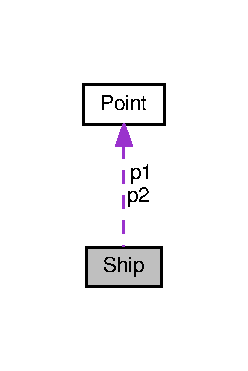
\includegraphics[width=119pt]{classMODEL_1_1Ship__coll__graph}
\end{center}
\end{figure}
\subsection*{Public Member Functions}
\begin{DoxyCompactItemize}
\item 
\hyperlink{classMODEL_1_1Ship_a8b83f3c2ed4f9097d7010a8f58b720e6}{Ship} (int \hyperlink{classMODEL_1_1Ship_a7441ef0865bcb3db9b8064dd7375c1ea}{id}, \hyperlink{classMODEL_1_1Point}{Point} \hyperlink{classMODEL_1_1Ship_ad513d6f843f1e0539132467d503e4591}{p1}, \hyperlink{classMODEL_1_1Point}{Point} \hyperlink{classMODEL_1_1Ship_a04aa64d0927f4422e811828cbe685358}{p2})
\item 
\hyperlink{classMODEL_1_1Ship_a5575ed570a5875b1c5828778b5d699aa}{Ship} (\hyperlink{classMODEL_1_1Ship}{Ship} const \&)=delete
\item 
\hyperlink{classMODEL_1_1Ship}{Ship} \& \hyperlink{classMODEL_1_1Ship_a00a328059de82741d06a9b59f599eb00}{operator=} (\hyperlink{classMODEL_1_1Ship}{Ship} const \&other)=delete
\item 
\hyperlink{classMODEL_1_1Ship_a8415fb9e85dd2049357fa6718d603516}{Ship} (\hyperlink{classMODEL_1_1Ship}{Ship} \&\&other)=delete
\item 
\hyperlink{classMODEL_1_1Ship}{Ship} \& \hyperlink{classMODEL_1_1Ship_a662d48126ddb24366430c841951c4760}{operator=} (\hyperlink{classMODEL_1_1Ship}{Ship} \&\&other)=delete
\end{DoxyCompactItemize}
\subsection*{Private Attributes}
\begin{DoxyCompactItemize}
\item 
int \hyperlink{classMODEL_1_1Ship_a7441ef0865bcb3db9b8064dd7375c1ea}{id}
\item 
\hyperlink{classMODEL_1_1Point}{Point} \hyperlink{classMODEL_1_1Ship_ad513d6f843f1e0539132467d503e4591}{p1}
\item 
\hyperlink{classMODEL_1_1Point}{Point} \hyperlink{classMODEL_1_1Ship_a04aa64d0927f4422e811828cbe685358}{p2}
\end{DoxyCompactItemize}


\subsection{Detailed Description}
A class representing a ship. 

\subsection{Constructor \& Destructor Documentation}
\index{M\+O\+D\+E\+L\+::\+Ship@{M\+O\+D\+E\+L\+::\+Ship}!Ship@{Ship}}
\index{Ship@{Ship}!M\+O\+D\+E\+L\+::\+Ship@{M\+O\+D\+E\+L\+::\+Ship}}
\subsubsection[{\texorpdfstring{Ship(int id, Point p1, Point p2)}{Ship(int id, Point p1, Point p2)}}]{\setlength{\rightskip}{0pt plus 5cm}{\bf Ship} (
\begin{DoxyParamCaption}
\item[{int}]{id, }
\item[{{\bf M\+O\+D\+E\+L\+::\+Point}}]{p1, }
\item[{{\bf M\+O\+D\+E\+L\+::\+Point}}]{p2}
\end{DoxyParamCaption}
)\hspace{0.3cm}{\ttfamily [explicit]}}\hypertarget{classMODEL_1_1Ship_a8b83f3c2ed4f9097d7010a8f58b720e6}{}\label{classMODEL_1_1Ship_a8b83f3c2ed4f9097d7010a8f58b720e6}
\index{M\+O\+D\+E\+L\+::\+Ship@{M\+O\+D\+E\+L\+::\+Ship}!Ship@{Ship}}
\index{Ship@{Ship}!M\+O\+D\+E\+L\+::\+Ship@{M\+O\+D\+E\+L\+::\+Ship}}
\subsubsection[{\texorpdfstring{Ship(\+Ship const \&)=delete}{Ship(Ship const &)=delete}}]{\setlength{\rightskip}{0pt plus 5cm}{\bf Ship} (
\begin{DoxyParamCaption}
\item[{{\bf Ship} const \&}]{}
\end{DoxyParamCaption}
)\hspace{0.3cm}{\ttfamily [delete]}}\hypertarget{classMODEL_1_1Ship_a5575ed570a5875b1c5828778b5d699aa}{}\label{classMODEL_1_1Ship_a5575ed570a5875b1c5828778b5d699aa}
\index{M\+O\+D\+E\+L\+::\+Ship@{M\+O\+D\+E\+L\+::\+Ship}!Ship@{Ship}}
\index{Ship@{Ship}!M\+O\+D\+E\+L\+::\+Ship@{M\+O\+D\+E\+L\+::\+Ship}}
\subsubsection[{\texorpdfstring{Ship(\+Ship \&\&other)=delete}{Ship(Ship &&other)=delete}}]{\setlength{\rightskip}{0pt plus 5cm}{\bf Ship} (
\begin{DoxyParamCaption}
\item[{{\bf Ship} \&\&}]{other}
\end{DoxyParamCaption}
)\hspace{0.3cm}{\ttfamily [delete]}}\hypertarget{classMODEL_1_1Ship_a8415fb9e85dd2049357fa6718d603516}{}\label{classMODEL_1_1Ship_a8415fb9e85dd2049357fa6718d603516}


\subsection{Member Function Documentation}
\index{M\+O\+D\+E\+L\+::\+Ship@{M\+O\+D\+E\+L\+::\+Ship}!operator=@{operator=}}
\index{operator=@{operator=}!M\+O\+D\+E\+L\+::\+Ship@{M\+O\+D\+E\+L\+::\+Ship}}
\subsubsection[{\texorpdfstring{operator=(\+Ship const \&other)=delete}{operator=(Ship const &other)=delete}}]{\setlength{\rightskip}{0pt plus 5cm}{\bf Ship}\& operator= (
\begin{DoxyParamCaption}
\item[{{\bf Ship} const \&}]{other}
\end{DoxyParamCaption}
)\hspace{0.3cm}{\ttfamily [delete]}}\hypertarget{classMODEL_1_1Ship_a00a328059de82741d06a9b59f599eb00}{}\label{classMODEL_1_1Ship_a00a328059de82741d06a9b59f599eb00}
\index{M\+O\+D\+E\+L\+::\+Ship@{M\+O\+D\+E\+L\+::\+Ship}!operator=@{operator=}}
\index{operator=@{operator=}!M\+O\+D\+E\+L\+::\+Ship@{M\+O\+D\+E\+L\+::\+Ship}}
\subsubsection[{\texorpdfstring{operator=(\+Ship \&\&other)=delete}{operator=(Ship &&other)=delete}}]{\setlength{\rightskip}{0pt plus 5cm}{\bf Ship}\& operator= (
\begin{DoxyParamCaption}
\item[{{\bf Ship} \&\&}]{other}
\end{DoxyParamCaption}
)\hspace{0.3cm}{\ttfamily [delete]}}\hypertarget{classMODEL_1_1Ship_a662d48126ddb24366430c841951c4760}{}\label{classMODEL_1_1Ship_a662d48126ddb24366430c841951c4760}


\subsection{Member Data Documentation}
\index{M\+O\+D\+E\+L\+::\+Ship@{M\+O\+D\+E\+L\+::\+Ship}!id@{id}}
\index{id@{id}!M\+O\+D\+E\+L\+::\+Ship@{M\+O\+D\+E\+L\+::\+Ship}}
\subsubsection[{\texorpdfstring{id}{id}}]{\setlength{\rightskip}{0pt plus 5cm}int id\hspace{0.3cm}{\ttfamily [private]}}\hypertarget{classMODEL_1_1Ship_a7441ef0865bcb3db9b8064dd7375c1ea}{}\label{classMODEL_1_1Ship_a7441ef0865bcb3db9b8064dd7375c1ea}
\index{M\+O\+D\+E\+L\+::\+Ship@{M\+O\+D\+E\+L\+::\+Ship}!p1@{p1}}
\index{p1@{p1}!M\+O\+D\+E\+L\+::\+Ship@{M\+O\+D\+E\+L\+::\+Ship}}
\subsubsection[{\texorpdfstring{p1}{p1}}]{\setlength{\rightskip}{0pt plus 5cm}{\bf Point} p1\hspace{0.3cm}{\ttfamily [private]}}\hypertarget{classMODEL_1_1Ship_ad513d6f843f1e0539132467d503e4591}{}\label{classMODEL_1_1Ship_ad513d6f843f1e0539132467d503e4591}
\index{M\+O\+D\+E\+L\+::\+Ship@{M\+O\+D\+E\+L\+::\+Ship}!p2@{p2}}
\index{p2@{p2}!M\+O\+D\+E\+L\+::\+Ship@{M\+O\+D\+E\+L\+::\+Ship}}
\subsubsection[{\texorpdfstring{p2}{p2}}]{\setlength{\rightskip}{0pt plus 5cm}{\bf Point} p2\hspace{0.3cm}{\ttfamily [private]}}\hypertarget{classMODEL_1_1Ship_a04aa64d0927f4422e811828cbe685358}{}\label{classMODEL_1_1Ship_a04aa64d0927f4422e811828cbe685358}


The documentation for this class was generated from the following files\+:\begin{DoxyCompactItemize}
\item 
model/\hyperlink{ship_8h}{ship.\+h}\item 
model/\hyperlink{ship_8cpp}{ship.\+cpp}\end{DoxyCompactItemize}

\hypertarget{classUserFriendlyException}{}\section{User\+Friendly\+Exception Class Reference}
\label{classUserFriendlyException}\index{User\+Friendly\+Exception@{User\+Friendly\+Exception}}


this kind of exception is intended to inform user with message in \hyperlink{namespaceGUI}{G\+UI} form, like Q\+Message\+Box  




{\ttfamily \#include $<$user\+\_\+friendly\+\_\+exception.\+h$>$}



Inheritance diagram for User\+Friendly\+Exception\+:\nopagebreak
\begin{figure}[H]
\begin{center}
\leavevmode
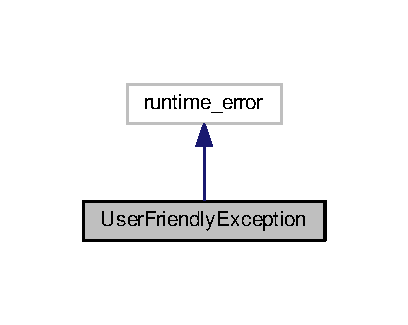
\includegraphics[width=196pt]{classUserFriendlyException__inherit__graph}
\end{center}
\end{figure}


Collaboration diagram for User\+Friendly\+Exception\+:\nopagebreak
\begin{figure}[H]
\begin{center}
\leavevmode
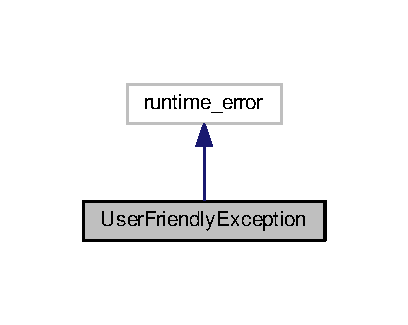
\includegraphics[width=196pt]{classUserFriendlyException__coll__graph}
\end{center}
\end{figure}
\subsection*{Public Member Functions}
\begin{DoxyCompactItemize}
\item 
\hyperlink{classUserFriendlyException_a4427d68327336a57cbe00b2d6dab91a6}{User\+Friendly\+Exception} (const std\+::string \&s)
\end{DoxyCompactItemize}


\subsection{Detailed Description}
this kind of exception is intended to inform user with message in \hyperlink{namespaceGUI}{G\+UI} form, like Q\+Message\+Box 

\subsection{Constructor \& Destructor Documentation}
\index{User\+Friendly\+Exception@{User\+Friendly\+Exception}!User\+Friendly\+Exception@{User\+Friendly\+Exception}}
\index{User\+Friendly\+Exception@{User\+Friendly\+Exception}!User\+Friendly\+Exception@{User\+Friendly\+Exception}}
\subsubsection[{\texorpdfstring{User\+Friendly\+Exception(const std\+::string \&s)}{UserFriendlyException(const std::string &s)}}]{\setlength{\rightskip}{0pt plus 5cm}{\bf User\+Friendly\+Exception} (
\begin{DoxyParamCaption}
\item[{const std\+::string \&}]{s}
\end{DoxyParamCaption}
)}\hypertarget{classUserFriendlyException_a4427d68327336a57cbe00b2d6dab91a6}{}\label{classUserFriendlyException_a4427d68327336a57cbe00b2d6dab91a6}


The documentation for this class was generated from the following files\+:\begin{DoxyCompactItemize}
\item 
common/\hyperlink{user__friendly__exception_8h}{user\+\_\+friendly\+\_\+exception.\+h}\item 
common/\hyperlink{user__friendly__exception_8cpp}{user\+\_\+friendly\+\_\+exception.\+cpp}\end{DoxyCompactItemize}

\hypertarget{classUserInfo}{}\section{User\+Info Class Reference}
\label{classUserInfo}\index{User\+Info@{User\+Info}}


A class which stores information about \hyperlink{classPlayer}{Player}.  




{\ttfamily \#include $<$user\+\_\+info.\+h$>$}

\subsection*{Public Member Functions}
\begin{DoxyCompactItemize}
\item 
\hyperlink{classUserInfo_a0ab18d3220b81916910df7a18f0c0236}{User\+Info} ()
\item 
\hyperlink{classUserInfo_a3c2608d1eafa1c8c459fb7cc6000afd0}{User\+Info} (const std\+::string \&\hyperlink{classUserInfo_a9b45b3e13bd9167aab02e17e08916231}{name}, int \hyperlink{classUserInfo_a91d98a856bbd96810b40af3ca5cc901a}{age})
\item 
\hyperlink{classUserInfo_ad304963be4e387d8b3bf289190a88010}{User\+Info} (const Q\+Json\+Object \&json)
\item 
Q\+Json\+Object \hyperlink{classUserInfo_a8cfaec036a21fc723e9cf94382891fa0}{to\+Json} () const 
\item 
const std\+::string \& \hyperlink{classUserInfo_aef436e6e20d1dbf2eb78b089ca9d0794}{get\+Name} () const 
\item 
int \hyperlink{classUserInfo_a3c04e615a5a30208ea6140e58c53709e}{get\+Age} () const 
\end{DoxyCompactItemize}
\subsection*{Private Attributes}
\begin{DoxyCompactItemize}
\item 
std\+::string \hyperlink{classUserInfo_a9b45b3e13bd9167aab02e17e08916231}{name}
\item 
int \hyperlink{classUserInfo_a91d98a856bbd96810b40af3ca5cc901a}{age}
\end{DoxyCompactItemize}


\subsection{Detailed Description}
A class which stores information about \hyperlink{classPlayer}{Player}. 

\subsection{Constructor \& Destructor Documentation}
\index{User\+Info@{User\+Info}!User\+Info@{User\+Info}}
\index{User\+Info@{User\+Info}!User\+Info@{User\+Info}}
\subsubsection[{\texorpdfstring{User\+Info()}{UserInfo()}}]{\setlength{\rightskip}{0pt plus 5cm}{\bf User\+Info} (
\begin{DoxyParamCaption}
{}
\end{DoxyParamCaption}
)}\hypertarget{classUserInfo_a0ab18d3220b81916910df7a18f0c0236}{}\label{classUserInfo_a0ab18d3220b81916910df7a18f0c0236}
\index{User\+Info@{User\+Info}!User\+Info@{User\+Info}}
\index{User\+Info@{User\+Info}!User\+Info@{User\+Info}}
\subsubsection[{\texorpdfstring{User\+Info(const std\+::string \&name, int age)}{UserInfo(const std::string &name, int age)}}]{\setlength{\rightskip}{0pt plus 5cm}{\bf User\+Info} (
\begin{DoxyParamCaption}
\item[{const std\+::string \&}]{name, }
\item[{int}]{age}
\end{DoxyParamCaption}
)}\hypertarget{classUserInfo_a3c2608d1eafa1c8c459fb7cc6000afd0}{}\label{classUserInfo_a3c2608d1eafa1c8c459fb7cc6000afd0}
\index{User\+Info@{User\+Info}!User\+Info@{User\+Info}}
\index{User\+Info@{User\+Info}!User\+Info@{User\+Info}}
\subsubsection[{\texorpdfstring{User\+Info(const Q\+Json\+Object \&json)}{UserInfo(const QJsonObject &json)}}]{\setlength{\rightskip}{0pt plus 5cm}{\bf User\+Info} (
\begin{DoxyParamCaption}
\item[{const Q\+Json\+Object \&}]{json}
\end{DoxyParamCaption}
)}\hypertarget{classUserInfo_ad304963be4e387d8b3bf289190a88010}{}\label{classUserInfo_ad304963be4e387d8b3bf289190a88010}


\subsection{Member Function Documentation}
\index{User\+Info@{User\+Info}!get\+Age@{get\+Age}}
\index{get\+Age@{get\+Age}!User\+Info@{User\+Info}}
\subsubsection[{\texorpdfstring{get\+Age() const }{getAge() const }}]{\setlength{\rightskip}{0pt plus 5cm}int get\+Age (
\begin{DoxyParamCaption}
{}
\end{DoxyParamCaption}
) const}\hypertarget{classUserInfo_a3c04e615a5a30208ea6140e58c53709e}{}\label{classUserInfo_a3c04e615a5a30208ea6140e58c53709e}
\index{User\+Info@{User\+Info}!get\+Name@{get\+Name}}
\index{get\+Name@{get\+Name}!User\+Info@{User\+Info}}
\subsubsection[{\texorpdfstring{get\+Name() const }{getName() const }}]{\setlength{\rightskip}{0pt plus 5cm}const std\+::string \& get\+Name (
\begin{DoxyParamCaption}
{}
\end{DoxyParamCaption}
) const}\hypertarget{classUserInfo_aef436e6e20d1dbf2eb78b089ca9d0794}{}\label{classUserInfo_aef436e6e20d1dbf2eb78b089ca9d0794}
\index{User\+Info@{User\+Info}!to\+Json@{to\+Json}}
\index{to\+Json@{to\+Json}!User\+Info@{User\+Info}}
\subsubsection[{\texorpdfstring{to\+Json() const }{toJson() const }}]{\setlength{\rightskip}{0pt plus 5cm}Q\+Json\+Object to\+Json (
\begin{DoxyParamCaption}
{}
\end{DoxyParamCaption}
) const}\hypertarget{classUserInfo_a8cfaec036a21fc723e9cf94382891fa0}{}\label{classUserInfo_a8cfaec036a21fc723e9cf94382891fa0}


\subsection{Member Data Documentation}
\index{User\+Info@{User\+Info}!age@{age}}
\index{age@{age}!User\+Info@{User\+Info}}
\subsubsection[{\texorpdfstring{age}{age}}]{\setlength{\rightskip}{0pt plus 5cm}int age\hspace{0.3cm}{\ttfamily [private]}}\hypertarget{classUserInfo_a91d98a856bbd96810b40af3ca5cc901a}{}\label{classUserInfo_a91d98a856bbd96810b40af3ca5cc901a}
\index{User\+Info@{User\+Info}!name@{name}}
\index{name@{name}!User\+Info@{User\+Info}}
\subsubsection[{\texorpdfstring{name}{name}}]{\setlength{\rightskip}{0pt plus 5cm}std\+::string name\hspace{0.3cm}{\ttfamily [private]}}\hypertarget{classUserInfo_a9b45b3e13bd9167aab02e17e08916231}{}\label{classUserInfo_a9b45b3e13bd9167aab02e17e08916231}


The documentation for this class was generated from the following files\+:\begin{DoxyCompactItemize}
\item 
common/\hyperlink{user__info_8h}{user\+\_\+info.\+h}\item 
common/\hyperlink{user__info_8cpp}{user\+\_\+info.\+cpp}\end{DoxyCompactItemize}

\chapter{File Documentation}
\hypertarget{battleship__controller_8cpp}{}\section{battleship\+\_\+controller.\+cpp File Reference}
\label{battleship__controller_8cpp}\index{battleship\+\_\+controller.\+cpp@{battleship\+\_\+controller.\+cpp}}
{\ttfamily \#include \char`\"{}battleship\+\_\+controller.\+h\char`\"{}}\\*
{\ttfamily \#include \char`\"{}common/user\+\_\+friendly\+\_\+exception.\+h\char`\"{}}\\*
{\ttfamily \#include $<$Q\+String$>$}\\*
{\ttfamily \#include \char`\"{}common/user\+\_\+info.\+h\char`\"{}}\\*
Include dependency graph for battleship\+\_\+controller.\+cpp\+:\nopagebreak
\begin{figure}[H]
\begin{center}
\leavevmode
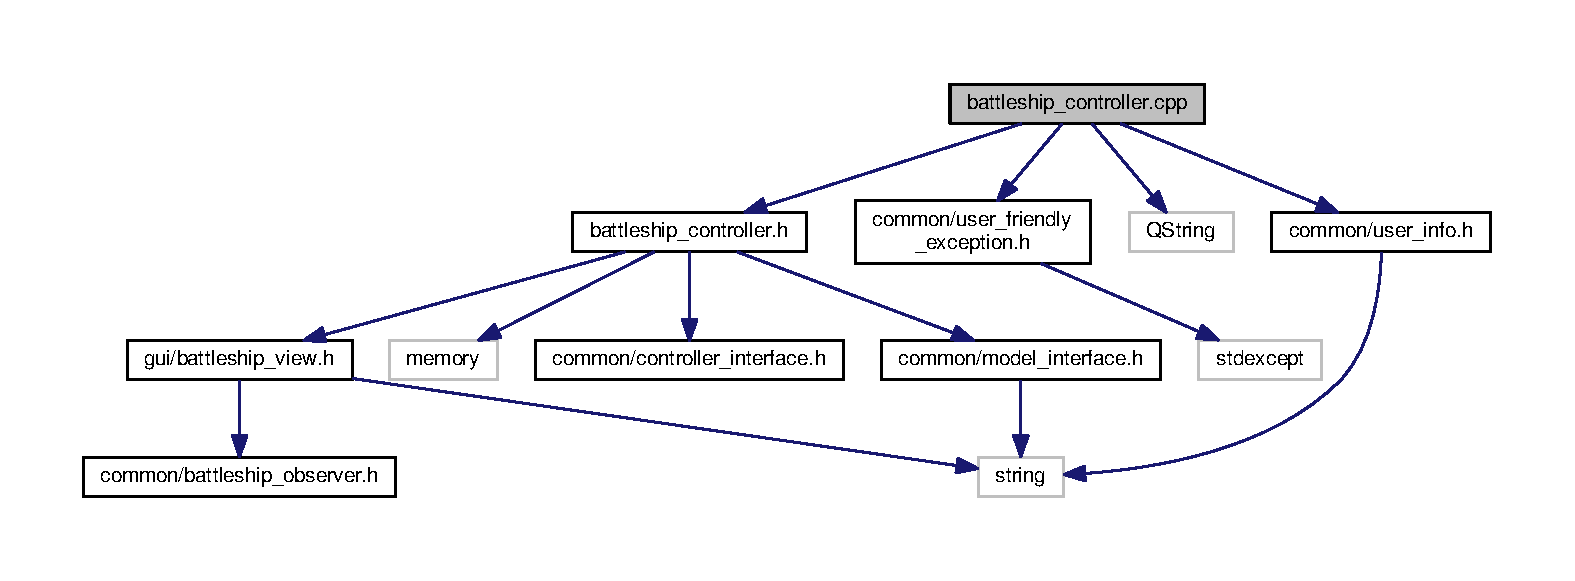
\includegraphics[width=350pt]{battleship__controller_8cpp__incl}
\end{center}
\end{figure}

\hypertarget{battleship__controller_8h}{}\section{battleship\+\_\+controller.\+h File Reference}
\label{battleship__controller_8h}\index{battleship\+\_\+controller.\+h@{battleship\+\_\+controller.\+h}}
{\ttfamily \#include \char`\"{}common/controller\+\_\+interface.\+h\char`\"{}}\\*
{\ttfamily \#include \char`\"{}common/model\+\_\+interface.\+h\char`\"{}}\\*
{\ttfamily \#include \char`\"{}gui/battleship\+\_\+view.\+h\char`\"{}}\\*
{\ttfamily \#include $<$memory$>$}\\*
Include dependency graph for battleship\+\_\+controller.\+h\+:\nopagebreak
\begin{figure}[H]
\begin{center}
\leavevmode
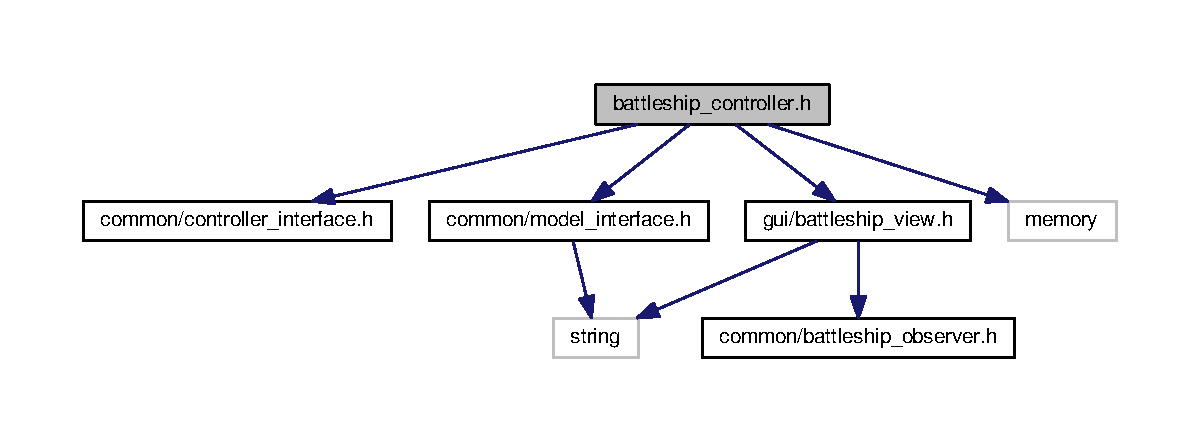
\includegraphics[width=350pt]{battleship__controller_8h__incl}
\end{center}
\end{figure}
This graph shows which files directly or indirectly include this file\+:\nopagebreak
\begin{figure}[H]
\begin{center}
\leavevmode
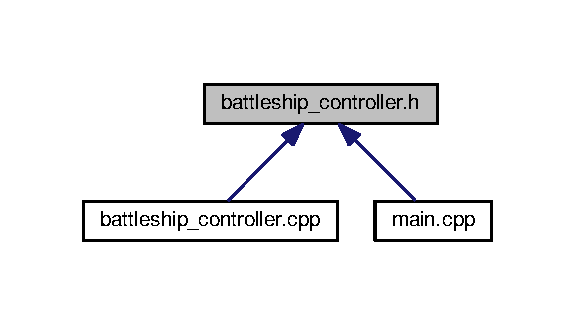
\includegraphics[width=276pt]{battleship__controller_8h__dep__incl}
\end{center}
\end{figure}
\subsection*{Classes}
\begin{DoxyCompactItemize}
\item 
class \hyperlink{classBattleshipController}{Battleship\+Controller}
\begin{DoxyCompactList}\small\item\em Provides model data to the view and interprets user actions. \end{DoxyCompactList}\end{DoxyCompactItemize}

\hypertarget{battleship__observer_8h}{}\section{common/battleship\+\_\+observer.h File Reference}
\label{battleship__observer_8h}\index{common/battleship\+\_\+observer.\+h@{common/battleship\+\_\+observer.\+h}}
This graph shows which files directly or indirectly include this file\+:\nopagebreak
\begin{figure}[H]
\begin{center}
\leavevmode
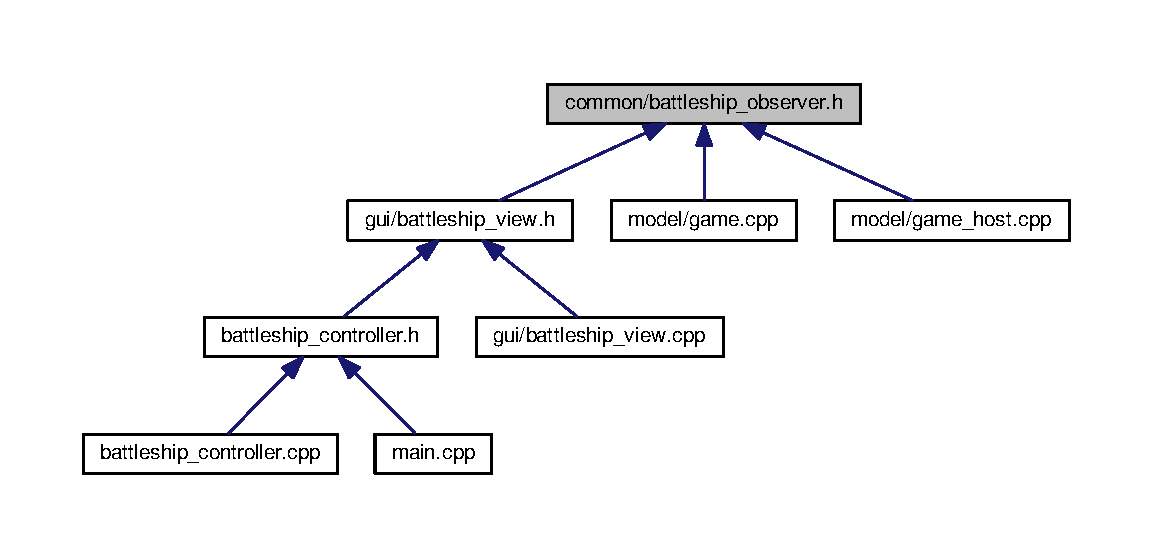
\includegraphics[width=350pt]{battleship__observer_8h__dep__incl}
\end{center}
\end{figure}
\subsection*{Classes}
\begin{DoxyCompactItemize}
\item 
class \hyperlink{classBattleshipObserver}{Battleship\+Observer}
\begin{DoxyCompactList}\small\item\em A base interface class, includes methods, which communicate with model and gui. \end{DoxyCompactList}\end{DoxyCompactItemize}

\hypertarget{controller__interface_8h}{}\section{common/controller\+\_\+interface.h File Reference}
\label{controller__interface_8h}\index{common/controller\+\_\+interface.\+h@{common/controller\+\_\+interface.\+h}}
This graph shows which files directly or indirectly include this file\+:\nopagebreak
\begin{figure}[H]
\begin{center}
\leavevmode
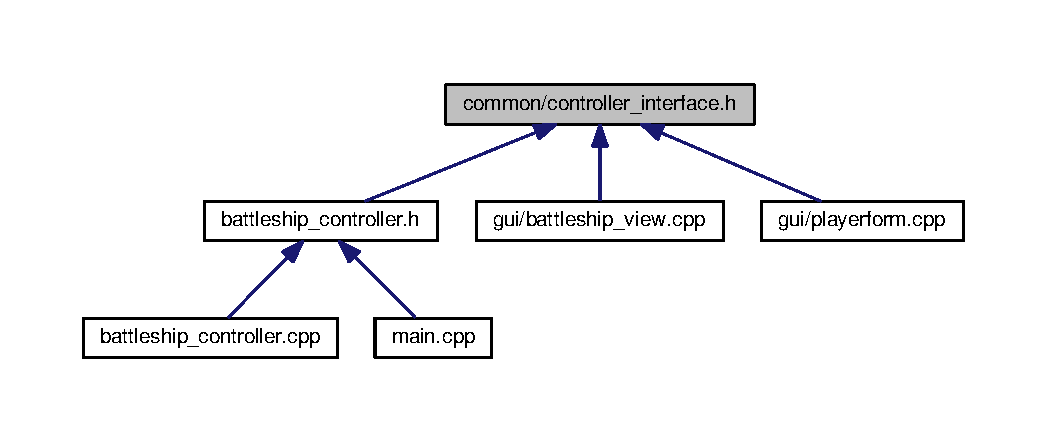
\includegraphics[width=350pt]{controller__interface_8h__dep__incl}
\end{center}
\end{figure}
\subsection*{Classes}
\begin{DoxyCompactItemize}
\item 
class \hyperlink{classControllerInterface}{Controller\+Interface}
\begin{DoxyCompactList}\small\item\em The base class that defines the controller interface. \end{DoxyCompactList}\end{DoxyCompactItemize}

\hypertarget{model__interface_8h}{}\section{common/model\+\_\+interface.h File Reference}
\label{model__interface_8h}\index{common/model\+\_\+interface.\+h@{common/model\+\_\+interface.\+h}}
{\ttfamily \#include $<$string$>$}\\*
Include dependency graph for model\+\_\+interface.\+h\+:\nopagebreak
\begin{figure}[H]
\begin{center}
\leavevmode
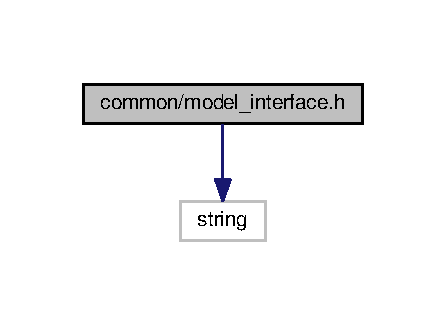
\includegraphics[width=214pt]{model__interface_8h__incl}
\end{center}
\end{figure}
This graph shows which files directly or indirectly include this file\+:\nopagebreak
\begin{figure}[H]
\begin{center}
\leavevmode
\includegraphics[width=350pt]{model__interface_8h__dep__incl}
\end{center}
\end{figure}
\subsection*{Classes}
\begin{DoxyCompactItemize}
\item 
class \hyperlink{classModelInterface}{Model\+Interface}
\begin{DoxyCompactList}\small\item\em The base class that defines the model interface. \end{DoxyCompactList}\end{DoxyCompactItemize}
\subsection*{Namespaces}
\begin{DoxyCompactItemize}
\item 
 \hyperlink{namespaceMODEL}{M\+O\+D\+EL}
\end{DoxyCompactItemize}

\hypertarget{user__friendly__exception_8cpp}{}\section{common/user\+\_\+friendly\+\_\+exception.cpp File Reference}
\label{user__friendly__exception_8cpp}\index{common/user\+\_\+friendly\+\_\+exception.\+cpp@{common/user\+\_\+friendly\+\_\+exception.\+cpp}}
{\ttfamily \#include \char`\"{}user\+\_\+friendly\+\_\+exception.\+h\char`\"{}}\\*
Include dependency graph for user\+\_\+friendly\+\_\+exception.\+cpp\+:\nopagebreak
\begin{figure}[H]
\begin{center}
\leavevmode
\includegraphics[width=208pt]{user__friendly__exception_8cpp__incl}
\end{center}
\end{figure}

\hypertarget{user__friendly__exception_8h}{}\section{common/user\+\_\+friendly\+\_\+exception.h File Reference}
\label{user__friendly__exception_8h}\index{common/user\+\_\+friendly\+\_\+exception.\+h@{common/user\+\_\+friendly\+\_\+exception.\+h}}
{\ttfamily \#include $<$stdexcept$>$}\\*
Include dependency graph for user\+\_\+friendly\+\_\+exception.\+h\+:\nopagebreak
\begin{figure}[H]
\begin{center}
\leavevmode
\includegraphics[width=193pt]{user__friendly__exception_8h__incl}
\end{center}
\end{figure}
This graph shows which files directly or indirectly include this file\+:\nopagebreak
\begin{figure}[H]
\begin{center}
\leavevmode
\includegraphics[width=350pt]{user__friendly__exception_8h__dep__incl}
\end{center}
\end{figure}
\subsection*{Classes}
\begin{DoxyCompactItemize}
\item 
class \hyperlink{classUserFriendlyException}{User\+Friendly\+Exception}
\begin{DoxyCompactList}\small\item\em this kind of exception is intended to inform user with message in \hyperlink{namespaceGUI}{G\+UI} form, like Q\+Message\+Box \end{DoxyCompactList}\end{DoxyCompactItemize}

\hypertarget{user__info_8cpp}{}\section{common/user\+\_\+info.cpp File Reference}
\label{user__info_8cpp}\index{common/user\+\_\+info.\+cpp@{common/user\+\_\+info.\+cpp}}
{\ttfamily \#include \char`\"{}user\+\_\+info.\+h\char`\"{}}\\*
{\ttfamily \#include $<$Q\+Json\+Object$>$}\\*
Include dependency graph for user\+\_\+info.\+cpp\+:\nopagebreak
\begin{figure}[H]
\begin{center}
\leavevmode
\includegraphics[width=238pt]{user__info_8cpp__incl}
\end{center}
\end{figure}

\hypertarget{user__info_8h}{}\section{common/user\+\_\+info.h File Reference}
\label{user__info_8h}\index{common/user\+\_\+info.\+h@{common/user\+\_\+info.\+h}}
{\ttfamily \#include $<$string$>$}\\*
Include dependency graph for user\+\_\+info.\+h\+:\nopagebreak
\begin{figure}[H]
\begin{center}
\leavevmode
\includegraphics[width=185pt]{user__info_8h__incl}
\end{center}
\end{figure}
This graph shows which files directly or indirectly include this file\+:\nopagebreak
\begin{figure}[H]
\begin{center}
\leavevmode
\includegraphics[width=350pt]{user__info_8h__dep__incl}
\end{center}
\end{figure}
\subsection*{Classes}
\begin{DoxyCompactItemize}
\item 
class \hyperlink{classUserInfo}{User\+Info}
\begin{DoxyCompactList}\small\item\em A class which stores information about \hyperlink{classPlayer}{Player}. \end{DoxyCompactList}\end{DoxyCompactItemize}

\hypertarget{battleship__view_8cpp}{}\section{gui/battleship\+\_\+view.cpp File Reference}
\label{battleship__view_8cpp}\index{gui/battleship\+\_\+view.\+cpp@{gui/battleship\+\_\+view.\+cpp}}
{\ttfamily \#include \char`\"{}battleship\+\_\+view.\+h\char`\"{}}\\*
{\ttfamily \#include \char`\"{}common/model\+\_\+interface.\+h\char`\"{}}\\*
{\ttfamily \#include \char`\"{}common/controller\+\_\+interface.\+h\char`\"{}}\\*
{\ttfamily \#include \char`\"{}playerform.\+h\char`\"{}}\\*
{\ttfamily \#include $<$Q\+Message\+Box$>$}\\*
{\ttfamily \#include $<$Q\+Debug$>$}\\*
Include dependency graph for battleship\+\_\+view.\+cpp\+:\nopagebreak
\begin{figure}[H]
\begin{center}
\leavevmode
\includegraphics[width=350pt]{battleship__view_8cpp__incl}
\end{center}
\end{figure}

\hypertarget{battleship__view_8h}{}\section{gui/battleship\+\_\+view.h File Reference}
\label{battleship__view_8h}\index{gui/battleship\+\_\+view.\+h@{gui/battleship\+\_\+view.\+h}}
{\ttfamily \#include $<$string$>$}\\*
{\ttfamily \#include \char`\"{}common/battleship\+\_\+observer.\+h\char`\"{}}\\*
Include dependency graph for battleship\+\_\+view.\+h\+:\nopagebreak
\begin{figure}[H]
\begin{center}
\leavevmode
\includegraphics[width=289pt]{battleship__view_8h__incl}
\end{center}
\end{figure}
This graph shows which files directly or indirectly include this file\+:\nopagebreak
\begin{figure}[H]
\begin{center}
\leavevmode
\includegraphics[width=350pt]{battleship__view_8h__dep__incl}
\end{center}
\end{figure}
\subsection*{Classes}
\begin{DoxyCompactItemize}
\item 
class \hyperlink{classGUI_1_1BattleshipView}{Battleship\+View}
\begin{DoxyCompactList}\small\item\em A simple class that defines and argument exception. \end{DoxyCompactList}\end{DoxyCompactItemize}
\subsection*{Namespaces}
\begin{DoxyCompactItemize}
\item 
 \hyperlink{namespaceGUI}{G\+UI}
\end{DoxyCompactItemize}

\hypertarget{coordinatesystem_8cpp}{}\section{gui/coordinatesystem.cpp File Reference}
\label{coordinatesystem_8cpp}\index{gui/coordinatesystem.\+cpp@{gui/coordinatesystem.\+cpp}}
{\ttfamily \#include \char`\"{}coordinatesystem.\+h\char`\"{}}\\*
{\ttfamily \#include $<$qpainter.\+h$>$}\\*
{\ttfamily \#include $<$iostream$>$}\\*
{\ttfamily \#include $<$Q\+Mouse\+Event$>$}\\*
{\ttfamily \#include $<$Q\+Graphics\+Scene\+Mouse\+Event$>$}\\*
{\ttfamily \#include $<$cmath$>$}\\*
{\ttfamily \#include $<$Q\+Debug$>$}\\*
Include dependency graph for coordinatesystem.\+cpp\+:\nopagebreak
\begin{figure}[H]
\begin{center}
\leavevmode
\includegraphics[width=350pt]{coordinatesystem_8cpp__incl}
\end{center}
\end{figure}

\hypertarget{coordinatesystem_8h}{}\section{gui/coordinatesystem.h File Reference}
\label{coordinatesystem_8h}\index{gui/coordinatesystem.\+h@{gui/coordinatesystem.\+h}}
{\ttfamily \#include $<$qwidget.\+h$>$}\\*
{\ttfamily \#include $<$Q\+Graphics\+View$>$}\\*
{\ttfamily \#include $<$memory$>$}\\*
Include dependency graph for coordinatesystem.\+h\+:\nopagebreak
\begin{figure}[H]
\begin{center}
\leavevmode
\includegraphics[width=313pt]{coordinatesystem_8h__incl}
\end{center}
\end{figure}
This graph shows which files directly or indirectly include this file\+:\nopagebreak
\begin{figure}[H]
\begin{center}
\leavevmode
\includegraphics[width=350pt]{coordinatesystem_8h__dep__incl}
\end{center}
\end{figure}
\subsection*{Classes}
\begin{DoxyCompactItemize}
\item 
class \hyperlink{classGUI_1_1CoordinateSystem}{Coordinate\+System}
\begin{DoxyCompactList}\small\item\em A virtual base class that defines the essential data for all coordinate systems. \end{DoxyCompactList}\end{DoxyCompactItemize}
\subsection*{Namespaces}
\begin{DoxyCompactItemize}
\item 
 \hyperlink{namespaceGUI}{G\+UI}
\end{DoxyCompactItemize}

\hypertarget{digitalclock_8cpp}{}\section{gui/digitalclock.cpp File Reference}
\label{digitalclock_8cpp}\index{gui/digitalclock.\+cpp@{gui/digitalclock.\+cpp}}
{\ttfamily \#include \char`\"{}digitalclock.\+h\char`\"{}}\\*
{\ttfamily \#include $<$Q\+Timer$>$}\\*
{\ttfamily \#include $<$Q\+Time$>$}\\*
{\ttfamily \#include $<$Q\+Message\+Box$>$}\\*
Include dependency graph for digitalclock.\+cpp\+:\nopagebreak
\begin{figure}[H]
\begin{center}
\leavevmode
\includegraphics[width=350pt]{digitalclock_8cpp__incl}
\end{center}
\end{figure}

\hypertarget{digitalclock_8h}{}\section{gui/digitalclock.h File Reference}
\label{digitalclock_8h}\index{gui/digitalclock.\+h@{gui/digitalclock.\+h}}
{\ttfamily \#include $<$Q\+L\+C\+D\+Number$>$}\\*
Include dependency graph for digitalclock.\+h\+:\nopagebreak
\begin{figure}[H]
\begin{center}
\leavevmode
\includegraphics[width=169pt]{digitalclock_8h__incl}
\end{center}
\end{figure}
This graph shows which files directly or indirectly include this file\+:\nopagebreak
\begin{figure}[H]
\begin{center}
\leavevmode
\includegraphics[width=294pt]{digitalclock_8h__dep__incl}
\end{center}
\end{figure}
\subsection*{Classes}
\begin{DoxyCompactItemize}
\item 
class \hyperlink{classDigitalClock}{Digital\+Clock}
\begin{DoxyCompactList}\small\item\em A class that defines the graphical interface for timer. \end{DoxyCompactList}\end{DoxyCompactItemize}

\hypertarget{gamecoordinatesystem_8cpp}{}\section{gui/gamecoordinatesystem.cpp File Reference}
\label{gamecoordinatesystem_8cpp}\index{gui/gamecoordinatesystem.\+cpp@{gui/gamecoordinatesystem.\+cpp}}
{\ttfamily \#include \char`\"{}gamecoordinatesystem.\+h\char`\"{}}\\*
{\ttfamily \#include $<$Q\+Debug$>$}\\*
{\ttfamily \#include $<$Q\+Mouse\+Event$>$}\\*
{\ttfamily \#include $<$Q\+Graphics\+Scene\+Mouse\+Event$>$}\\*
{\ttfamily \#include $<$Q\+Line$>$}\\*
Include dependency graph for gamecoordinatesystem.\+cpp\+:\nopagebreak
\begin{figure}[H]
\begin{center}
\leavevmode
\includegraphics[width=350pt]{gamecoordinatesystem_8cpp__incl}
\end{center}
\end{figure}

\hypertarget{gamecoordinatesystem_8h}{}\section{gui/gamecoordinatesystem.h File Reference}
\label{gamecoordinatesystem_8h}\index{gui/gamecoordinatesystem.\+h@{gui/gamecoordinatesystem.\+h}}
{\ttfamily \#include \char`\"{}coordinatesystem.\+h\char`\"{}}\\*
{\ttfamily \#include $<$qwidget.\+h$>$}\\*
{\ttfamily \#include $<$Q\+Graphics\+View$>$}\\*
{\ttfamily \#include $<$memory$>$}\\*
{\ttfamily \#include $<$Q\+Line$>$}\\*
Include dependency graph for gamecoordinatesystem.\+h\+:\nopagebreak
\begin{figure}[H]
\begin{center}
\leavevmode
\includegraphics[width=350pt]{gamecoordinatesystem_8h__incl}
\end{center}
\end{figure}
This graph shows which files directly or indirectly include this file\+:\nopagebreak
\begin{figure}[H]
\begin{center}
\leavevmode
\includegraphics[width=350pt]{gamecoordinatesystem_8h__dep__incl}
\end{center}
\end{figure}
\subsection*{Classes}
\begin{DoxyCompactItemize}
\item 
class \hyperlink{classGUI_1_1GameCoordinateSystem}{Game\+Coordinate\+System}
\begin{DoxyCompactList}\small\item\em A simple class that inherits from \hyperlink{classGUI_1_1CoordinateSystem}{Coordinate\+System} and implements mouse events for starting attack. \end{DoxyCompactList}\end{DoxyCompactItemize}
\subsection*{Namespaces}
\begin{DoxyCompactItemize}
\item 
 \hyperlink{namespaceGUI}{G\+UI}
\end{DoxyCompactItemize}

\hypertarget{gameform_8cpp}{}\section{gui/gameform.cpp File Reference}
\label{gameform_8cpp}\index{gui/gameform.\+cpp@{gui/gameform.\+cpp}}
{\ttfamily \#include \char`\"{}gameform.\+h\char`\"{}}\\*
{\ttfamily \#include $<$Qt\+Widgets$>$}\\*
{\ttfamily \#include \char`\"{}digitalclock.\+h\char`\"{}}\\*
{\ttfamily \#include \char`\"{}gamecoordinatesystem.\+h\char`\"{}}\\*
Include dependency graph for gameform.\+cpp\+:\nopagebreak
\begin{figure}[H]
\begin{center}
\leavevmode
\includegraphics[width=350pt]{gameform_8cpp__incl}
\end{center}
\end{figure}

\hypertarget{gameform_8h}{}\section{gui/gameform.h File Reference}
\label{gameform_8h}\index{gui/gameform.\+h@{gui/gameform.\+h}}
{\ttfamily \#include $<$Q\+Dialog$>$}\\*
{\ttfamily \#include $<$Q\+Text\+Edit$>$}\\*
{\ttfamily \#include $<$Q\+Grid\+Layout$>$}\\*
{\ttfamily \#include \char`\"{}coordinatesystem.\+h\char`\"{}}\\*
{\ttfamily \#include \char`\"{}gamecoordinatesystem.\+h\char`\"{}}\\*
Include dependency graph for gameform.\+h\+:\nopagebreak
\begin{figure}[H]
\begin{center}
\leavevmode
\includegraphics[width=350pt]{gameform_8h__incl}
\end{center}
\end{figure}
This graph shows which files directly or indirectly include this file\+:\nopagebreak
\begin{figure}[H]
\begin{center}
\leavevmode
\includegraphics[width=300pt]{gameform_8h__dep__incl}
\end{center}
\end{figure}
\subsection*{Classes}
\begin{DoxyCompactItemize}
\item 
class \hyperlink{classGameForm}{Game\+Form}
\begin{DoxyCompactList}\small\item\em A simple class that defines graphical interface of the form in which players are able to attack, recieve attack, etc. \end{DoxyCompactList}\end{DoxyCompactItemize}

\hypertarget{gui_2player_8cpp}{}\section{gui/player.cpp File Reference}
\label{gui_2player_8cpp}\index{gui/player.\+cpp@{gui/player.\+cpp}}
{\ttfamily \#include \char`\"{}player.\+h\char`\"{}}\\*
{\ttfamily \#include \char`\"{}Q\+String\char`\"{}}\\*
{\ttfamily \#include \char`\"{}Q\+Message\+Box\char`\"{}}\\*
{\ttfamily \#include \char`\"{}Q\+List\char`\"{}}\\*
Include dependency graph for player.\+cpp\+:\nopagebreak
\begin{figure}[H]
\begin{center}
\leavevmode
\includegraphics[width=312pt]{gui_2player_8cpp__incl}
\end{center}
\end{figure}

\hypertarget{model_2player_8cpp}{}\section{model/player.cpp File Reference}
\label{model_2player_8cpp}\index{model/player.\+cpp@{model/player.\+cpp}}
{\ttfamily \#include \char`\"{}player.\+h\char`\"{}}\\*
Include dependency graph for player.\+cpp\+:\nopagebreak
\begin{figure}[H]
\begin{center}
\leavevmode
\includegraphics[width=310pt]{model_2player_8cpp__incl}
\end{center}
\end{figure}

\hypertarget{gui_2player_8h}{}\section{gui/player.h File Reference}
\label{gui_2player_8h}\index{gui/player.\+h@{gui/player.\+h}}
{\ttfamily \#include $<$Q\+String$>$}\\*
{\ttfamily \#include $<$Q\+List$>$}\\*
Include dependency graph for player.\+h\+:\nopagebreak
\begin{figure}[H]
\begin{center}
\leavevmode
\includegraphics[width=188pt]{gui_2player_8h__incl}
\end{center}
\end{figure}
This graph shows which files directly or indirectly include this file\+:\nopagebreak
\begin{figure}[H]
\begin{center}
\leavevmode
\includegraphics[width=350pt]{gui_2player_8h__dep__incl}
\end{center}
\end{figure}
\subsection*{Classes}
\begin{DoxyCompactItemize}
\item 
class \hyperlink{classPlayer}{Player}
\begin{DoxyCompactList}\small\item\em A class representing player for graphical interface. \end{DoxyCompactList}\end{DoxyCompactItemize}

\hypertarget{model_2player_8h}{}\section{model/player.h File Reference}
\label{model_2player_8h}\index{model/player.\+h@{model/player.\+h}}
{\ttfamily \#include \char`\"{}common/user\+\_\+info.\+h\char`\"{}}\\*
{\ttfamily \#include \char`\"{}coordinate\+\_\+system.\+h\char`\"{}}\\*
Include dependency graph for player.\+h\+:\nopagebreak
\begin{figure}[H]
\begin{center}
\leavevmode
\includegraphics[width=310pt]{model_2player_8h__incl}
\end{center}
\end{figure}
This graph shows which files directly or indirectly include this file\+:\nopagebreak
\begin{figure}[H]
\begin{center}
\leavevmode
\includegraphics[width=350pt]{model_2player_8h__dep__incl}
\end{center}
\end{figure}
\subsection*{Classes}
\begin{DoxyCompactItemize}
\item 
class \hyperlink{classMODEL_1_1Player}{Player}
\begin{DoxyCompactList}\small\item\em A class representing player for model, stores information in \hyperlink{classUserInfo}{User\+Info} object within it. \end{DoxyCompactList}\end{DoxyCompactItemize}
\subsection*{Namespaces}
\begin{DoxyCompactItemize}
\item 
 \hyperlink{namespaceMODEL}{M\+O\+D\+EL}
\end{DoxyCompactItemize}

\hypertarget{playerform_8cpp}{}\section{gui/playerform.cpp File Reference}
\label{playerform_8cpp}\index{gui/playerform.\+cpp@{gui/playerform.\+cpp}}
{\ttfamily \#include $<$Qt\+Widgets$>$}\\*
{\ttfamily \#include \char`\"{}playerform.\+h\char`\"{}}\\*
{\ttfamily \#include \char`\"{}setshipsform.\+h\char`\"{}}\\*
{\ttfamily \#include \char`\"{}common/controller\+\_\+interface.\+h\char`\"{}}\\*
Include dependency graph for playerform.\+cpp\+:\nopagebreak
\begin{figure}[H]
\begin{center}
\leavevmode
\includegraphics[width=350pt]{playerform_8cpp__incl}
\end{center}
\end{figure}

\hypertarget{playerform_8h}{}\section{gui/playerform.h File Reference}
\label{playerform_8h}\index{gui/playerform.\+h@{gui/playerform.\+h}}
{\ttfamily \#include \char`\"{}player.\+h\char`\"{}}\\*
{\ttfamily \#include $<$Q\+Dialog$>$}\\*
Include dependency graph for playerform.\+h\+:\nopagebreak
\begin{figure}[H]
\begin{center}
\leavevmode
\includegraphics[width=232pt]{playerform_8h__incl}
\end{center}
\end{figure}
This graph shows which files directly or indirectly include this file\+:\nopagebreak
\begin{figure}[H]
\begin{center}
\leavevmode
\includegraphics[width=314pt]{playerform_8h__dep__incl}
\end{center}
\end{figure}
\subsection*{Classes}
\begin{DoxyCompactItemize}
\item 
class \hyperlink{classGUI_1_1PlayerForm}{Player\+Form}
\begin{DoxyCompactList}\small\item\em A simple class that defines graphical interface of the form in which players are able enter the name and age. \end{DoxyCompactList}\end{DoxyCompactItemize}
\subsection*{Namespaces}
\begin{DoxyCompactItemize}
\item 
 \hyperlink{namespaceGUI}{G\+UI}
\end{DoxyCompactItemize}

\hypertarget{setshipsform_8cpp}{}\section{gui/setshipsform.cpp File Reference}
\label{setshipsform_8cpp}\index{gui/setshipsform.\+cpp@{gui/setshipsform.\+cpp}}
{\ttfamily \#include $<$Qt\+Widgets$>$}\\*
{\ttfamily \#include \char`\"{}setshipsform.\+h\char`\"{}}\\*
{\ttfamily \#include \char`\"{}gameform.\+h\char`\"{}}\\*
{\ttfamily \#include \char`\"{}player.\+h\char`\"{}}\\*
{\ttfamily \#include $<$Q\+String$>$}\\*
Include dependency graph for setshipsform.\+cpp\+:\nopagebreak
\begin{figure}[H]
\begin{center}
\leavevmode
\includegraphics[width=350pt]{setshipsform_8cpp__incl}
\end{center}
\end{figure}

\hypertarget{setshipsform_8h}{}\section{gui/setshipsform.h File Reference}
\label{setshipsform_8h}\index{gui/setshipsform.\+h@{gui/setshipsform.\+h}}
{\ttfamily \#include $<$Q\+Dialog$>$}\\*
{\ttfamily \#include \char`\"{}coordinatesystem.\+h\char`\"{}}\\*
{\ttfamily \#include \char`\"{}settingshipscoordinatesystem.\+h\char`\"{}}\\*
{\ttfamily \#include \char`\"{}player.\+h\char`\"{}}\\*
Include dependency graph for setshipsform.\+h\+:\nopagebreak
\begin{figure}[H]
\begin{center}
\leavevmode
\includegraphics[width=350pt]{setshipsform_8h__incl}
\end{center}
\end{figure}
This graph shows which files directly or indirectly include this file\+:\nopagebreak
\begin{figure}[H]
\begin{center}
\leavevmode
\includegraphics[width=302pt]{setshipsform_8h__dep__incl}
\end{center}
\end{figure}
\subsection*{Classes}
\begin{DoxyCompactItemize}
\item 
class \hyperlink{classSetShipsForm}{Set\+Ships\+Form}
\begin{DoxyCompactList}\small\item\em A simple class that defines graphical interface of the form in which players are able to set ships. \end{DoxyCompactList}\end{DoxyCompactItemize}

\hypertarget{settingshipscoordinatesystem_8cpp}{}\section{gui/settingshipscoordinatesystem.cpp File Reference}
\label{settingshipscoordinatesystem_8cpp}\index{gui/settingshipscoordinatesystem.\+cpp@{gui/settingshipscoordinatesystem.\+cpp}}
{\ttfamily \#include \char`\"{}settingshipscoordinatesystem.\+h\char`\"{}}\\*
{\ttfamily \#include $<$qpainter.\+h$>$}\\*
{\ttfamily \#include $<$iostream$>$}\\*
{\ttfamily \#include $<$Q\+Mouse\+Event$>$}\\*
{\ttfamily \#include $<$Q\+Graphics\+Scene\+Mouse\+Event$>$}\\*
{\ttfamily \#include $<$cmath$>$}\\*
{\ttfamily \#include $<$Q\+Debug$>$}\\*
Include dependency graph for settingshipscoordinatesystem.\+cpp\+:\nopagebreak
\begin{figure}[H]
\begin{center}
\leavevmode
\includegraphics[width=350pt]{settingshipscoordinatesystem_8cpp__incl}
\end{center}
\end{figure}

\hypertarget{settingshipscoordinatesystem_8h}{}\section{gui/settingshipscoordinatesystem.h File Reference}
\label{settingshipscoordinatesystem_8h}\index{gui/settingshipscoordinatesystem.\+h@{gui/settingshipscoordinatesystem.\+h}}
{\ttfamily \#include $<$qwidget.\+h$>$}\\*
{\ttfamily \#include $<$Q\+Graphics\+View$>$}\\*
{\ttfamily \#include $<$memory$>$}\\*
{\ttfamily \#include \char`\"{}coordinatesystem.\+h\char`\"{}}\\*
Include dependency graph for settingshipscoordinatesystem.\+h\+:\nopagebreak
\begin{figure}[H]
\begin{center}
\leavevmode
\includegraphics[width=327pt]{settingshipscoordinatesystem_8h__incl}
\end{center}
\end{figure}
This graph shows which files directly or indirectly include this file\+:\nopagebreak
\begin{figure}[H]
\begin{center}
\leavevmode
\includegraphics[width=350pt]{settingshipscoordinatesystem_8h__dep__incl}
\end{center}
\end{figure}
\subsection*{Classes}
\begin{DoxyCompactItemize}
\item 
class \hyperlink{classGUI_1_1SettingShipsCoordinateSystem}{Setting\+Ships\+Coordinate\+System}
\begin{DoxyCompactList}\small\item\em A simple class that inherits from \hyperlink{classGUI_1_1CoordinateSystem}{Coordinate\+System} and implements mouse events for setting ships. \end{DoxyCompactList}\end{DoxyCompactItemize}
\subsection*{Namespaces}
\begin{DoxyCompactItemize}
\item 
 \hyperlink{namespaceGUI}{G\+UI}
\end{DoxyCompactItemize}

\hypertarget{main_8cpp}{}\section{main.\+cpp File Reference}
\label{main_8cpp}\index{main.\+cpp@{main.\+cpp}}
{\ttfamily \#include $<$Q\+Application$>$}\\*
{\ttfamily \#include \char`\"{}model/battleship\+\_\+model.\+h\char`\"{}}\\*
{\ttfamily \#include \char`\"{}battleship\+\_\+controller.\+h\char`\"{}}\\*
Include dependency graph for main.\+cpp\+:\nopagebreak
\begin{figure}[H]
\begin{center}
\leavevmode
\includegraphics[width=350pt]{main_8cpp__incl}
\end{center}
\end{figure}
\subsection*{Functions}
\begin{DoxyCompactItemize}
\item 
int \hyperlink{main_8cpp_a0ddf1224851353fc92bfbff6f499fa97}{main} (int argc, char $\ast$argv\mbox{[}$\,$\mbox{]})
\end{DoxyCompactItemize}


\subsection{Function Documentation}
\index{main.\+cpp@{main.\+cpp}!main@{main}}
\index{main@{main}!main.\+cpp@{main.\+cpp}}
\subsubsection[{\texorpdfstring{main(int argc, char $\ast$argv[])}{main(int argc, char *argv[])}}]{\setlength{\rightskip}{0pt plus 5cm}int main (
\begin{DoxyParamCaption}
\item[{int}]{argc, }
\item[{char $\ast$}]{argv\mbox{[}$\,$\mbox{]}}
\end{DoxyParamCaption}
)}\hypertarget{main_8cpp_a0ddf1224851353fc92bfbff6f499fa97}{}\label{main_8cpp_a0ddf1224851353fc92bfbff6f499fa97}

\hypertarget{battleship__model_8cpp}{}\section{model/battleship\+\_\+model.cpp File Reference}
\label{battleship__model_8cpp}\index{model/battleship\+\_\+model.\+cpp@{model/battleship\+\_\+model.\+cpp}}
{\ttfamily \#include \char`\"{}battleship\+\_\+model.\+h\char`\"{}}\\*
{\ttfamily \#include \char`\"{}game\+\_\+guest.\+h\char`\"{}}\\*
{\ttfamily \#include \char`\"{}game\+\_\+host.\+h\char`\"{}}\\*
{\ttfamily \#include \char`\"{}common/user\+\_\+info.\+h\char`\"{}}\\*
{\ttfamily \#include \char`\"{}point.\+h\char`\"{}}\\*
Include dependency graph for battleship\+\_\+model.\+cpp\+:\nopagebreak
\begin{figure}[H]
\begin{center}
\leavevmode
\includegraphics[width=350pt]{battleship__model_8cpp__incl}
\end{center}
\end{figure}

\hypertarget{battleship__model_8h}{}\section{model/battleship\+\_\+model.h File Reference}
\label{battleship__model_8h}\index{model/battleship\+\_\+model.\+h@{model/battleship\+\_\+model.\+h}}
{\ttfamily \#include \char`\"{}common/model\+\_\+interface.\+h\char`\"{}}\\*
{\ttfamily \#include $<$memory$>$}\\*
{\ttfamily \#include $<$vector$>$}\\*
{\ttfamily \#include $<$functional$>$}\\*
{\ttfamily \#include \char`\"{}game.\+h\char`\"{}}\\*
Include dependency graph for battleship\+\_\+model.\+h\+:\nopagebreak
\begin{figure}[H]
\begin{center}
\leavevmode
\includegraphics[width=350pt]{battleship__model_8h__incl}
\end{center}
\end{figure}
This graph shows which files directly or indirectly include this file\+:\nopagebreak
\begin{figure}[H]
\begin{center}
\leavevmode
\includegraphics[width=292pt]{battleship__model_8h__dep__incl}
\end{center}
\end{figure}
\subsection*{Classes}
\begin{DoxyCompactItemize}
\item 
class \hyperlink{classMODEL_1_1BattleshipModel}{Battleship\+Model}
\begin{DoxyCompactList}\small\item\em acts primarely as a wrapper around \hyperlink{classMODEL_1_1Game}{M\+O\+D\+E\+L\+::\+Game} class. Especially we make use of its constructor \& destructor. And we can dynamicallly switch between Host and Guest if so desired \end{DoxyCompactList}\end{DoxyCompactItemize}
\subsection*{Namespaces}
\begin{DoxyCompactItemize}
\item 
 \hyperlink{namespaceMODEL}{M\+O\+D\+EL}
\end{DoxyCompactItemize}

\hypertarget{communicator_8cpp}{}\section{model/communicator.cpp File Reference}
\label{communicator_8cpp}\index{model/communicator.\+cpp@{model/communicator.\+cpp}}
{\ttfamily \#include \char`\"{}communicator.\+h\char`\"{}}\\*
{\ttfamily \#include \char`\"{}game.\+h\char`\"{}}\\*
{\ttfamily \#include \char`\"{}connection\+\_\+guest.\+h\char`\"{}}\\*
{\ttfamily \#include \char`\"{}connection\+\_\+host.\+h\char`\"{}}\\*
{\ttfamily \#include $<$memory$>$}\\*
{\ttfamily \#include $<$Q\+Json\+Object$>$}\\*
{\ttfamily \#include $<$Q\+Json\+Document$>$}\\*
{\ttfamily \#include \char`\"{}common/user\+\_\+info.\+h\char`\"{}}\\*
Include dependency graph for communicator.\+cpp\+:\nopagebreak
\begin{figure}[H]
\begin{center}
\leavevmode
\includegraphics[width=350pt]{communicator_8cpp__incl}
\end{center}
\end{figure}

\hypertarget{communicator_8h}{}\section{model/communicator.h File Reference}
\label{communicator_8h}\index{model/communicator.\+h@{model/communicator.\+h}}
{\ttfamily \#include $<$memory$>$}\\*
{\ttfamily \#include $<$Q\+Json\+Array$>$}\\*
{\ttfamily \#include $<$Q\+Json\+Object$>$}\\*
{\ttfamily \#include $<$Q\+Json\+Document$>$}\\*
{\ttfamily \#include \char`\"{}connection.\+h\char`\"{}}\\*
Include dependency graph for communicator.\+h\+:\nopagebreak
\begin{figure}[H]
\begin{center}
\leavevmode
\includegraphics[width=350pt]{communicator_8h__incl}
\end{center}
\end{figure}
This graph shows which files directly or indirectly include this file\+:\nopagebreak
\begin{figure}[H]
\begin{center}
\leavevmode
\includegraphics[width=350pt]{communicator_8h__dep__incl}
\end{center}
\end{figure}
\subsection*{Classes}
\begin{DoxyCompactItemize}
\item 
class \hyperlink{classMODEL_1_1Communicator}{Communicator}
\begin{DoxyCompactList}\small\item\em A class that uses \hyperlink{classMODEL_1_1Connection}{Connection} to recieve/send encoded/decoded information stored in json objects. \end{DoxyCompactList}\end{DoxyCompactItemize}
\subsection*{Namespaces}
\begin{DoxyCompactItemize}
\item 
 \hyperlink{namespaceMODEL}{M\+O\+D\+EL}
\end{DoxyCompactItemize}
\subsection*{Enumerations}
\begin{DoxyCompactItemize}
\item 
enum \hyperlink{namespaceMODEL_a2afce0a47a93eee73a314d53e4890153}{Command} \{ \hyperlink{namespaceMODEL_a2afce0a47a93eee73a314d53e4890153a53e95d4aedd7db4fe9f58af71525d56a}{U\+S\+E\+R\+\_\+\+I\+N\+FO}, 
\hyperlink{namespaceMODEL_a2afce0a47a93eee73a314d53e4890153a8f686af5a9b889f9a227dfd8862a81d4}{S\+H\+I\+P\+\_\+\+P\+L\+A\+C\+E\+M\+E\+NT}
 \}
\end{DoxyCompactItemize}

\hypertarget{connection_8cpp}{}\section{model/connection.cpp File Reference}
\label{connection_8cpp}\index{model/connection.\+cpp@{model/connection.\+cpp}}
{\ttfamily \#include \char`\"{}connection.\+h\char`\"{}}\\*
{\ttfamily \#include $<$Q\+Network\+Configuration\+Manager$>$}\\*
{\ttfamily \#include $<$Q\+Settings$>$}\\*
{\ttfamily \#include $<$Q\+Network\+Session$>$}\\*
{\ttfamily \#include $<$Q\+Data\+Stream$>$}\\*
{\ttfamily \#include $<$Q\+Tcp\+Socket$>$}\\*
Include dependency graph for connection.\+cpp\+:\nopagebreak
\begin{figure}[H]
\begin{center}
\leavevmode
\includegraphics[width=350pt]{connection_8cpp__incl}
\end{center}
\end{figure}

\hypertarget{connection_8h}{}\section{model/connection.h File Reference}
\label{connection_8h}\index{model/connection.\+h@{model/connection.\+h}}
{\ttfamily \#include $<$Q\+Object$>$}\\*
{\ttfamily \#include $<$Q\+Abstract\+Socket$>$}\\*
{\ttfamily \#include $<$vector$>$}\\*
{\ttfamily \#include $<$functional$>$}\\*
Include dependency graph for connection.\+h\+:\nopagebreak
\begin{figure}[H]
\begin{center}
\leavevmode
\includegraphics[width=350pt]{connection_8h__incl}
\end{center}
\end{figure}
This graph shows which files directly or indirectly include this file\+:\nopagebreak
\begin{figure}[H]
\begin{center}
\leavevmode
\includegraphics[width=350pt]{connection_8h__dep__incl}
\end{center}
\end{figure}
\subsection*{Classes}
\begin{DoxyCompactItemize}
\item 
class \hyperlink{classMODEL_1_1Connection}{Connection}
\begin{DoxyCompactList}\small\item\em A base class that defines the basic functions for connection. \end{DoxyCompactList}\end{DoxyCompactItemize}
\subsection*{Namespaces}
\begin{DoxyCompactItemize}
\item 
 \hyperlink{namespaceMODEL}{M\+O\+D\+EL}
\end{DoxyCompactItemize}

\hypertarget{connection__guest_8cpp}{}\section{model/connection\+\_\+guest.cpp File Reference}
\label{connection__guest_8cpp}\index{model/connection\+\_\+guest.\+cpp@{model/connection\+\_\+guest.\+cpp}}
{\ttfamily \#include \char`\"{}connection\+\_\+guest.\+h\char`\"{}}\\*
{\ttfamily \#include $<$Q\+Data\+Stream$>$}\\*
{\ttfamily \#include $<$Q\+Network\+Configuration\+Manager$>$}\\*
{\ttfamily \#include $<$Q\+Settings$>$}\\*
{\ttfamily \#include $<$Q\+Network\+Session$>$}\\*
Include dependency graph for connection\+\_\+guest.\+cpp\+:\nopagebreak
\begin{figure}[H]
\begin{center}
\leavevmode
\includegraphics[width=350pt]{connection__guest_8cpp__incl}
\end{center}
\end{figure}

\hypertarget{connection__guest_8h}{}\section{model/connection\+\_\+guest.h File Reference}
\label{connection__guest_8h}\index{model/connection\+\_\+guest.\+h@{model/connection\+\_\+guest.\+h}}
{\ttfamily \#include \char`\"{}connection.\+h\char`\"{}}\\*
{\ttfamily \#include $<$string$>$}\\*
{\ttfamily \#include $<$Q\+Tcp\+Socket$>$}\\*
{\ttfamily \#include $<$Q\+Abstract\+Socket$>$}\\*
Include dependency graph for connection\+\_\+guest.\+h\+:\nopagebreak
\begin{figure}[H]
\begin{center}
\leavevmode
\includegraphics[width=350pt]{connection__guest_8h__incl}
\end{center}
\end{figure}
This graph shows which files directly or indirectly include this file\+:\nopagebreak
\begin{figure}[H]
\begin{center}
\leavevmode
\includegraphics[width=350pt]{connection__guest_8h__dep__incl}
\end{center}
\end{figure}
\subsection*{Classes}
\begin{DoxyCompactItemize}
\item 
class \hyperlink{classMODEL_1_1ConnectionGuest}{Connection\+Guest}
\begin{DoxyCompactList}\small\item\em Inherits from \hyperlink{classMODEL_1_1Connection}{Connection} and implements the functionality for connection used by guest. \end{DoxyCompactList}\end{DoxyCompactItemize}
\subsection*{Namespaces}
\begin{DoxyCompactItemize}
\item 
 \hyperlink{namespaceMODEL}{M\+O\+D\+EL}
\end{DoxyCompactItemize}

\hypertarget{connection__host_8cpp}{}\section{model/connection\+\_\+host.cpp File Reference}
\label{connection__host_8cpp}\index{model/connection\+\_\+host.\+cpp@{model/connection\+\_\+host.\+cpp}}
{\ttfamily \#include \char`\"{}connection\+\_\+host.\+h\char`\"{}}\\*
{\ttfamily \#include \char`\"{}common/user\+\_\+friendly\+\_\+exception.\+h\char`\"{}}\\*
{\ttfamily \#include $<$Q\+Network\+Configuration\+Manager$>$}\\*
{\ttfamily \#include $<$Q\+Settings$>$}\\*
{\ttfamily \#include $<$Q\+Network\+Session$>$}\\*
{\ttfamily \#include $<$Q\+Tcp\+Socket$>$}\\*
{\ttfamily \#include $<$Q\+Tcp\+Server$>$}\\*
{\ttfamily \#include $<$Q\+Data\+Stream$>$}\\*
Include dependency graph for connection\+\_\+host.\+cpp\+:\nopagebreak
\begin{figure}[H]
\begin{center}
\leavevmode
\includegraphics[width=350pt]{connection__host_8cpp__incl}
\end{center}
\end{figure}

\hypertarget{connection__host_8h}{}\section{model/connection\+\_\+host.h File Reference}
\label{connection__host_8h}\index{model/connection\+\_\+host.\+h@{model/connection\+\_\+host.\+h}}
{\ttfamily \#include \char`\"{}connection.\+h\char`\"{}}\\*
Include dependency graph for connection\+\_\+host.\+h\+:\nopagebreak
\begin{figure}[H]
\begin{center}
\leavevmode
\includegraphics[width=350pt]{connection__host_8h__incl}
\end{center}
\end{figure}
This graph shows which files directly or indirectly include this file\+:\nopagebreak
\begin{figure}[H]
\begin{center}
\leavevmode
\includegraphics[width=350pt]{connection__host_8h__dep__incl}
\end{center}
\end{figure}
\subsection*{Classes}
\begin{DoxyCompactItemize}
\item 
class \hyperlink{classMODEL_1_1ConnectionHost}{Connection\+Host}
\begin{DoxyCompactList}\small\item\em Inherits from \hyperlink{classMODEL_1_1Connection}{Connection} and implements the functionality for connection used by host. \end{DoxyCompactList}\end{DoxyCompactItemize}
\subsection*{Namespaces}
\begin{DoxyCompactItemize}
\item 
 \hyperlink{namespaceMODEL}{M\+O\+D\+EL}
\end{DoxyCompactItemize}

\hypertarget{coordinate__system_8cpp}{}\section{model/coordinate\+\_\+system.cpp File Reference}
\label{coordinate__system_8cpp}\index{model/coordinate\+\_\+system.\+cpp@{model/coordinate\+\_\+system.\+cpp}}
{\ttfamily \#include \char`\"{}coordinate\+\_\+system.\+h\char`\"{}}\\*
{\ttfamily \#include $<$stdexcept$>$}\\*
Include dependency graph for coordinate\+\_\+system.\+cpp\+:\nopagebreak
\begin{figure}[H]
\begin{center}
\leavevmode
\includegraphics[width=264pt]{coordinate__system_8cpp__incl}
\end{center}
\end{figure}

\hypertarget{coordinate__system_8h}{}\section{model/coordinate\+\_\+system.h File Reference}
\label{coordinate__system_8h}\index{model/coordinate\+\_\+system.\+h@{model/coordinate\+\_\+system.\+h}}
{\ttfamily \#include $<$deque$>$}\\*
{\ttfamily \#include \char`\"{}ship.\+h\char`\"{}}\\*
Include dependency graph for coordinate\+\_\+system.\+h\+:\nopagebreak
\begin{figure}[H]
\begin{center}
\leavevmode
\includegraphics[width=217pt]{coordinate__system_8h__incl}
\end{center}
\end{figure}
This graph shows which files directly or indirectly include this file\+:\nopagebreak
\begin{figure}[H]
\begin{center}
\leavevmode
\includegraphics[width=350pt]{coordinate__system_8h__dep__incl}
\end{center}
\end{figure}
\subsection*{Classes}
\begin{DoxyCompactItemize}
\item 
class \hyperlink{classMODEL_1_1CoordinateSystem}{Coordinate\+System}
\begin{DoxyCompactList}\small\item\em A class that stores data of coordinate system separately from the graphical interface. \end{DoxyCompactList}\end{DoxyCompactItemize}
\subsection*{Namespaces}
\begin{DoxyCompactItemize}
\item 
 \hyperlink{namespaceMODEL}{M\+O\+D\+EL}
\end{DoxyCompactItemize}

\hypertarget{game_8cpp}{}\section{model/game.cpp File Reference}
\label{game_8cpp}\index{model/game.\+cpp@{model/game.\+cpp}}
{\ttfamily \#include \char`\"{}game.\+h\char`\"{}}\\*
{\ttfamily \#include $<$Q\+Debug$>$}\\*
{\ttfamily \#include \char`\"{}common/battleship\+\_\+observer.\+h\char`\"{}}\\*
{\ttfamily \#include \char`\"{}common/user\+\_\+info.\+h\char`\"{}}\\*
{\ttfamily \#include \char`\"{}point.\+h\char`\"{}}\\*
Include dependency graph for game.\+cpp\+:\nopagebreak
\begin{figure}[H]
\begin{center}
\leavevmode
\includegraphics[width=350pt]{game_8cpp__incl}
\end{center}
\end{figure}

\hypertarget{game_8h}{}\section{model/game.h File Reference}
\label{game_8h}\index{model/game.\+h@{model/game.\+h}}
{\ttfamily \#include \char`\"{}communicator.\+h\char`\"{}}\\*
{\ttfamily \#include \char`\"{}model/player.\+h\char`\"{}}\\*
Include dependency graph for game.\+h\+:\nopagebreak
\begin{figure}[H]
\begin{center}
\leavevmode
\includegraphics[width=350pt]{game_8h__incl}
\end{center}
\end{figure}
This graph shows which files directly or indirectly include this file\+:\nopagebreak
\begin{figure}[H]
\begin{center}
\leavevmode
\includegraphics[width=350pt]{game_8h__dep__incl}
\end{center}
\end{figure}
\subsection*{Classes}
\begin{DoxyCompactItemize}
\item 
class \hyperlink{classMODEL_1_1Game}{Game}
\begin{DoxyCompactList}\small\item\em A class representing game session that access both \hyperlink{classMODEL_1_1Player}{Player} and \hyperlink{classMODEL_1_1Communicator}{Communicator}. \end{DoxyCompactList}\end{DoxyCompactItemize}
\subsection*{Namespaces}
\begin{DoxyCompactItemize}
\item 
 \hyperlink{namespaceMODEL}{M\+O\+D\+EL}
\end{DoxyCompactItemize}

\hypertarget{game__guest_8cpp}{}\section{model/game\+\_\+guest.cpp File Reference}
\label{game__guest_8cpp}\index{model/game\+\_\+guest.\+cpp@{model/game\+\_\+guest.\+cpp}}
{\ttfamily \#include \char`\"{}game\+\_\+guest.\+h\char`\"{}}\\*
{\ttfamily \#include \char`\"{}common/user\+\_\+info.\+h\char`\"{}}\\*
Include dependency graph for game\+\_\+guest.\+cpp\+:\nopagebreak
\begin{figure}[H]
\begin{center}
\leavevmode
\includegraphics[width=350pt]{game__guest_8cpp__incl}
\end{center}
\end{figure}

\hypertarget{game__guest_8h}{}\section{model/game\+\_\+guest.h File Reference}
\label{game__guest_8h}\index{model/game\+\_\+guest.\+h@{model/game\+\_\+guest.\+h}}
{\ttfamily \#include \char`\"{}game.\+h\char`\"{}}\\*
{\ttfamily \#include \char`\"{}connection\+\_\+guest.\+h\char`\"{}}\\*
Include dependency graph for game\+\_\+guest.\+h\+:\nopagebreak
\begin{figure}[H]
\begin{center}
\leavevmode
\includegraphics[width=350pt]{game__guest_8h__incl}
\end{center}
\end{figure}
This graph shows which files directly or indirectly include this file\+:\nopagebreak
\begin{figure}[H]
\begin{center}
\leavevmode
\includegraphics[width=350pt]{game__guest_8h__dep__incl}
\end{center}
\end{figure}
\subsection*{Classes}
\begin{DoxyCompactItemize}
\item 
class \hyperlink{classMODEL_1_1GameGuest}{Game\+Guest}
\begin{DoxyCompactList}\small\item\em Inherits \hyperlink{classMODEL_1_1Game}{Game} and make it possible to manage guests game. \end{DoxyCompactList}\end{DoxyCompactItemize}
\subsection*{Namespaces}
\begin{DoxyCompactItemize}
\item 
 \hyperlink{namespaceMODEL}{M\+O\+D\+EL}
\end{DoxyCompactItemize}

\hypertarget{game__host_8cpp}{}\section{model/game\+\_\+host.cpp File Reference}
\label{game__host_8cpp}\index{model/game\+\_\+host.\+cpp@{model/game\+\_\+host.\+cpp}}
{\ttfamily \#include \char`\"{}game\+\_\+host.\+h\char`\"{}}\\*
{\ttfamily \#include $<$Q\+Debug$>$}\\*
{\ttfamily \#include \char`\"{}common/battleship\+\_\+observer.\+h\char`\"{}}\\*
{\ttfamily \#include \char`\"{}common/user\+\_\+info.\+h\char`\"{}}\\*
Include dependency graph for game\+\_\+host.\+cpp\+:\nopagebreak
\begin{figure}[H]
\begin{center}
\leavevmode
\includegraphics[width=350pt]{game__host_8cpp__incl}
\end{center}
\end{figure}

\hypertarget{game__host_8h}{}\section{model/game\+\_\+host.h File Reference}
\label{game__host_8h}\index{model/game\+\_\+host.\+h@{model/game\+\_\+host.\+h}}
{\ttfamily \#include \char`\"{}game.\+h\char`\"{}}\\*
{\ttfamily \#include \char`\"{}connection\+\_\+host.\+h\char`\"{}}\\*
Include dependency graph for game\+\_\+host.\+h\+:\nopagebreak
\begin{figure}[H]
\begin{center}
\leavevmode
\includegraphics[width=350pt]{game__host_8h__incl}
\end{center}
\end{figure}
This graph shows which files directly or indirectly include this file\+:\nopagebreak
\begin{figure}[H]
\begin{center}
\leavevmode
\includegraphics[width=350pt]{game__host_8h__dep__incl}
\end{center}
\end{figure}
\subsection*{Classes}
\begin{DoxyCompactItemize}
\item 
class \hyperlink{classMODEL_1_1GameHost}{Game\+Host}
\begin{DoxyCompactList}\small\item\em Inherits \hyperlink{classMODEL_1_1Game}{Game} and make it possible to manage hosts game. \end{DoxyCompactList}\end{DoxyCompactItemize}
\subsection*{Namespaces}
\begin{DoxyCompactItemize}
\item 
 \hyperlink{namespaceMODEL}{M\+O\+D\+EL}
\end{DoxyCompactItemize}

\hypertarget{point_8cpp}{}\section{model/point.cpp File Reference}
\label{point_8cpp}\index{model/point.\+cpp@{model/point.\+cpp}}
{\ttfamily \#include \char`\"{}point.\+h\char`\"{}}\\*
Include dependency graph for point.\+cpp\+:\nopagebreak
\begin{figure}[H]
\begin{center}
\leavevmode
\includegraphics[width=166pt]{point_8cpp__incl}
\end{center}
\end{figure}

\hypertarget{point_8h}{}\section{model/point.h File Reference}
\label{point_8h}\index{model/point.\+h@{model/point.\+h}}
This graph shows which files directly or indirectly include this file\+:\nopagebreak
\begin{figure}[H]
\begin{center}
\leavevmode
\includegraphics[width=350pt]{point_8h__dep__incl}
\end{center}
\end{figure}
\subsection*{Classes}
\begin{DoxyCompactItemize}
\item 
class \hyperlink{classMODEL_1_1Point}{Point}
\begin{DoxyCompactList}\small\item\em A simple class representing point. \end{DoxyCompactList}\end{DoxyCompactItemize}
\subsection*{Namespaces}
\begin{DoxyCompactItemize}
\item 
 \hyperlink{namespaceMODEL}{M\+O\+D\+EL}
\end{DoxyCompactItemize}

\hypertarget{ship_8cpp}{}\section{model/ship.cpp File Reference}
\label{ship_8cpp}\index{model/ship.\+cpp@{model/ship.\+cpp}}
{\ttfamily \#include \char`\"{}ship.\+h\char`\"{}}\\*
Include dependency graph for ship.\+cpp\+:\nopagebreak
\begin{figure}[H]
\begin{center}
\leavevmode
\includegraphics[width=163pt]{ship_8cpp__incl}
\end{center}
\end{figure}

\hypertarget{ship_8h}{}\section{model/ship.h File Reference}
\label{ship_8h}\index{model/ship.\+h@{model/ship.\+h}}
{\ttfamily \#include \char`\"{}point.\+h\char`\"{}}\\*
Include dependency graph for ship.\+h\+:\nopagebreak
\begin{figure}[H]
\begin{center}
\leavevmode
\includegraphics[width=152pt]{ship_8h__incl}
\end{center}
\end{figure}
This graph shows which files directly or indirectly include this file\+:\nopagebreak
\begin{figure}[H]
\begin{center}
\leavevmode
\includegraphics[width=350pt]{ship_8h__dep__incl}
\end{center}
\end{figure}
\subsection*{Classes}
\begin{DoxyCompactItemize}
\item 
class \hyperlink{classMODEL_1_1Ship}{Ship}
\begin{DoxyCompactList}\small\item\em A class representing a ship. \end{DoxyCompactList}\end{DoxyCompactItemize}
\subsection*{Namespaces}
\begin{DoxyCompactItemize}
\item 
 \hyperlink{namespaceMODEL}{M\+O\+D\+EL}
\end{DoxyCompactItemize}

\hypertarget{test__connection_8cpp}{}\section{test\+\_\+connection.\+cpp File Reference}
\label{test__connection_8cpp}\index{test\+\_\+connection.\+cpp@{test\+\_\+connection.\+cpp}}
{\ttfamily \#include $<$gtest/gtest.\+h$>$}\\*
{\ttfamily \#include $<$iostream$>$}\\*
{\ttfamily \#include \char`\"{}model/connection\+\_\+host.\+h\char`\"{}}\\*
Include dependency graph for test\+\_\+connection.\+cpp\+:\nopagebreak
\begin{figure}[H]
\begin{center}
\leavevmode
\includegraphics[width=350pt]{test__connection_8cpp__incl}
\end{center}
\end{figure}
\subsection*{Classes}
\begin{DoxyCompactItemize}
\item 
class \hyperlink{classConnectionTest}{Connection\+Test}
\end{DoxyCompactItemize}
\subsection*{Functions}
\begin{DoxyCompactItemize}
\item 
\hyperlink{test__connection_8cpp_a29e2983d254b5f7c0098d812965cbc81}{T\+E\+S\+T\+\_\+F} (\hyperlink{classConnectionTest}{Connection\+Test}, \hyperlink{classConnectionTest}{Connection\+Test})
\end{DoxyCompactItemize}


\subsection{Function Documentation}
\index{test\+\_\+connection.\+cpp@{test\+\_\+connection.\+cpp}!T\+E\+S\+T\+\_\+F@{T\+E\+S\+T\+\_\+F}}
\index{T\+E\+S\+T\+\_\+F@{T\+E\+S\+T\+\_\+F}!test\+\_\+connection.\+cpp@{test\+\_\+connection.\+cpp}}
\subsubsection[{\texorpdfstring{T\+E\+S\+T\+\_\+\+F(\+Connection\+Test, Connection\+Test)}{TEST_F(ConnectionTest, ConnectionTest)}}]{\setlength{\rightskip}{0pt plus 5cm}T\+E\+S\+T\+\_\+F (
\begin{DoxyParamCaption}
\item[{{\bf Connection\+Test}}]{, }
\item[{{\bf Connection\+Test}}]{}
\end{DoxyParamCaption}
)}\hypertarget{test__connection_8cpp_a29e2983d254b5f7c0098d812965cbc81}{}\label{test__connection_8cpp_a29e2983d254b5f7c0098d812965cbc81}

\hypertarget{test__model_8cpp}{}\section{test\+\_\+model.\+cpp File Reference}
\label{test__model_8cpp}\index{test\+\_\+model.\+cpp@{test\+\_\+model.\+cpp}}
{\ttfamily \#include \char`\"{}gtest/gtest.\+h\char`\"{}}\\*
{\ttfamily \#include $<$iostream$>$}\\*
Include dependency graph for test\+\_\+model.\+cpp\+:\nopagebreak
\begin{figure}[H]
\begin{center}
\leavevmode
\includegraphics[width=224pt]{test__model_8cpp__incl}
\end{center}
\end{figure}
\subsection*{Classes}
\begin{DoxyCompactItemize}
\item 
class \hyperlink{classModelTest}{Model\+Test}
\end{DoxyCompactItemize}
\subsection*{Functions}
\begin{DoxyCompactItemize}
\item 
\hyperlink{test__model_8cpp_ad79c9e89435b690a2abb9a43bbf5c475}{T\+E\+S\+T\+\_\+F} (\hyperlink{classModelTest}{Model\+Test}, Just\+Some\+Test)
\item 
\hyperlink{test__model_8cpp_a05f4bafe79de70bffc806cd5b8ebd117}{T\+E\+S\+T\+\_\+F} (\hyperlink{classModelTest}{Model\+Test}, Just\+Some\+Other\+Test)
\end{DoxyCompactItemize}


\subsection{Function Documentation}
\index{test\+\_\+model.\+cpp@{test\+\_\+model.\+cpp}!T\+E\+S\+T\+\_\+F@{T\+E\+S\+T\+\_\+F}}
\index{T\+E\+S\+T\+\_\+F@{T\+E\+S\+T\+\_\+F}!test\+\_\+model.\+cpp@{test\+\_\+model.\+cpp}}
\subsubsection[{\texorpdfstring{T\+E\+S\+T\+\_\+\+F(\+Model\+Test, Just\+Some\+Test)}{TEST_F(ModelTest, JustSomeTest)}}]{\setlength{\rightskip}{0pt plus 5cm}T\+E\+S\+T\+\_\+F (
\begin{DoxyParamCaption}
\item[{{\bf Model\+Test}}]{, }
\item[{Just\+Some\+Test}]{}
\end{DoxyParamCaption}
)}\hypertarget{test__model_8cpp_ad79c9e89435b690a2abb9a43bbf5c475}{}\label{test__model_8cpp_ad79c9e89435b690a2abb9a43bbf5c475}
\index{test\+\_\+model.\+cpp@{test\+\_\+model.\+cpp}!T\+E\+S\+T\+\_\+F@{T\+E\+S\+T\+\_\+F}}
\index{T\+E\+S\+T\+\_\+F@{T\+E\+S\+T\+\_\+F}!test\+\_\+model.\+cpp@{test\+\_\+model.\+cpp}}
\subsubsection[{\texorpdfstring{T\+E\+S\+T\+\_\+\+F(\+Model\+Test, Just\+Some\+Other\+Test)}{TEST_F(ModelTest, JustSomeOtherTest)}}]{\setlength{\rightskip}{0pt plus 5cm}T\+E\+S\+T\+\_\+F (
\begin{DoxyParamCaption}
\item[{{\bf Model\+Test}}]{, }
\item[{Just\+Some\+Other\+Test}]{}
\end{DoxyParamCaption}
)}\hypertarget{test__model_8cpp_a05f4bafe79de70bffc806cd5b8ebd117}{}\label{test__model_8cpp_a05f4bafe79de70bffc806cd5b8ebd117}

%--- End generated contents ---

% Index
\backmatter
\newpage
\phantomsection
\clearemptydoublepage
\addcontentsline{toc}{chapter}{Index}
\printindex

\end{document}
